% Options for packages loaded elsewhere
% Options for packages loaded elsewhere
\PassOptionsToPackage{unicode}{hyperref}
\PassOptionsToPackage{hyphens}{url}
%
\documentclass[
  ignorenonframetext,
]{beamer}
\newif\ifbibliography
\usepackage{pgfpages}
\setbeamertemplate{caption}[numbered]
\setbeamertemplate{caption label separator}{: }
\setbeamercolor{caption name}{fg=normal text.fg}
\beamertemplatenavigationsymbolsempty
% remove section numbering
\setbeamertemplate{part page}{
  \centering
  \begin{beamercolorbox}[sep=16pt,center]{part title}
    \usebeamerfont{part title}\insertpart\par
  \end{beamercolorbox}
}
\setbeamertemplate{section page}{
  \centering
  \begin{beamercolorbox}[sep=12pt,center]{section title}
    \usebeamerfont{section title}\insertsection\par
  \end{beamercolorbox}
}
\setbeamertemplate{subsection page}{
  \centering
  \begin{beamercolorbox}[sep=8pt,center]{subsection title}
    \usebeamerfont{subsection title}\insertsubsection\par
  \end{beamercolorbox}
}
% Prevent slide breaks in the middle of a paragraph
\widowpenalties 1 10000
\raggedbottom
\AtBeginPart{
  \frame{\partpage}
}
\AtBeginSection{
  \ifbibliography
  \else
    \frame{\sectionpage}
  \fi
}
\AtBeginSubsection{
  \frame{\subsectionpage}
}
\usepackage{iftex}
\ifPDFTeX
  \usepackage[T1]{fontenc}
  \usepackage[utf8]{inputenc}
  \usepackage{textcomp} % provide euro and other symbols
\else % if luatex or xetex
  \usepackage{unicode-math} % this also loads fontspec
  \defaultfontfeatures{Scale=MatchLowercase}
  \defaultfontfeatures[\rmfamily]{Ligatures=TeX,Scale=1}
\fi
\usepackage{lmodern}

\ifPDFTeX\else
  % xetex/luatex font selection
\fi
% Use upquote if available, for straight quotes in verbatim environments
\IfFileExists{upquote.sty}{\usepackage{upquote}}{}
\IfFileExists{microtype.sty}{% use microtype if available
  \usepackage[]{microtype}
  \UseMicrotypeSet[protrusion]{basicmath} % disable protrusion for tt fonts
}{}
\makeatletter
\@ifundefined{KOMAClassName}{% if non-KOMA class
  \IfFileExists{parskip.sty}{%
    \usepackage{parskip}
  }{% else
    \setlength{\parindent}{0pt}
    \setlength{\parskip}{6pt plus 2pt minus 1pt}}
}{% if KOMA class
  \KOMAoptions{parskip=half}}
\makeatother


\usepackage{longtable,booktabs,array}
\usepackage{calc} % for calculating minipage widths
\usepackage{caption}
% Make caption package work with longtable
\makeatletter
\def\fnum@table{\tablename~\thetable}
\makeatother
\usepackage{graphicx}
\makeatletter
\newsavebox\pandoc@box
\newcommand*\pandocbounded[1]{% scales image to fit in text height/width
  \sbox\pandoc@box{#1}%
  \Gscale@div\@tempa{\textheight}{\dimexpr\ht\pandoc@box+\dp\pandoc@box\relax}%
  \Gscale@div\@tempb{\linewidth}{\wd\pandoc@box}%
  \ifdim\@tempb\p@<\@tempa\p@\let\@tempa\@tempb\fi% select the smaller of both
  \ifdim\@tempa\p@<\p@\scalebox{\@tempa}{\usebox\pandoc@box}%
  \else\usebox{\pandoc@box}%
  \fi%
}
% Set default figure placement to htbp
\def\fps@figure{htbp}
\makeatother





\setlength{\emergencystretch}{3em} % prevent overfull lines

\providecommand{\tightlist}{%
  \setlength{\itemsep}{0pt}\setlength{\parskip}{0pt}}



 


\makeatletter
\@ifpackageloaded{tcolorbox}{}{\usepackage[skins,breakable]{tcolorbox}}
\@ifpackageloaded{fontawesome5}{}{\usepackage{fontawesome5}}
\definecolor{quarto-callout-color}{HTML}{909090}
\definecolor{quarto-callout-note-color}{HTML}{0758E5}
\definecolor{quarto-callout-important-color}{HTML}{CC1914}
\definecolor{quarto-callout-warning-color}{HTML}{EB9113}
\definecolor{quarto-callout-tip-color}{HTML}{00A047}
\definecolor{quarto-callout-caution-color}{HTML}{FC5300}
\definecolor{quarto-callout-color-frame}{HTML}{acacac}
\definecolor{quarto-callout-note-color-frame}{HTML}{4582ec}
\definecolor{quarto-callout-important-color-frame}{HTML}{d9534f}
\definecolor{quarto-callout-warning-color-frame}{HTML}{f0ad4e}
\definecolor{quarto-callout-tip-color-frame}{HTML}{02b875}
\definecolor{quarto-callout-caution-color-frame}{HTML}{fd7e14}
\makeatother
\makeatletter
\@ifpackageloaded{caption}{}{\usepackage{caption}}
\AtBeginDocument{%
\ifdefined\contentsname
  \renewcommand*\contentsname{Table of contents}
\else
  \newcommand\contentsname{Table of contents}
\fi
\ifdefined\listfigurename
  \renewcommand*\listfigurename{List of Figures}
\else
  \newcommand\listfigurename{List of Figures}
\fi
\ifdefined\listtablename
  \renewcommand*\listtablename{List of Tables}
\else
  \newcommand\listtablename{List of Tables}
\fi
\ifdefined\figurename
  \renewcommand*\figurename{Figure}
\else
  \newcommand\figurename{Figure}
\fi
\ifdefined\tablename
  \renewcommand*\tablename{Table}
\else
  \newcommand\tablename{Table}
\fi
}
\@ifpackageloaded{float}{}{\usepackage{float}}
\floatstyle{ruled}
\@ifundefined{c@chapter}{\newfloat{codelisting}{h}{lop}}{\newfloat{codelisting}{h}{lop}[chapter]}
\floatname{codelisting}{Listing}
\newcommand*\listoflistings{\listof{codelisting}{List of Listings}}
\makeatother
\makeatletter
\makeatother
\makeatletter
\@ifpackageloaded{caption}{}{\usepackage{caption}}
\@ifpackageloaded{subcaption}{}{\usepackage{subcaption}}
\makeatother

\usepackage{bookmark}
\IfFileExists{xurl.sty}{\usepackage{xurl}}{} % add URL line breaks if available
\urlstyle{same}
\hypersetup{
  pdftitle={Tema 6: Grafos y árboles soporte},
  pdfauthor={Víctor Aceña Gil - Antonio Alonso Ayuso},
  hidelinks,
  pdfcreator={LaTeX via pandoc}}


\title{Tema 6: Grafos y árboles soporte}
\subtitle{Optimización y Análisis de Redes}
\author{Víctor Aceña Gil - Antonio Alonso Ayuso}
\date{2026-08-07}

\begin{document}
\frame{\titlepage}


\begin{frame}{Objetivos de aprendizaje}
\phantomsection\label{objetivos-de-aprendizaje}
\begin{enumerate}
\tightlist
\item
  \textbf{Definir} grafos dirigidos y no dirigidos, vecindades, grados e
  incidencias de corte.
\item
  \textbf{Diferenciar} cadenas, caminos, ciclos y circuitos, y
  clasificar la conexidad en digrafos.
\item
  \textbf{Caracterizar} grafos planares y bipartitos mediante Euler,
  Dudeney y Kuratowski.
\item
  \textbf{Formular} matrices de adyacencia e incidencia (TUM), vectores
  (\(\alpha, \beta\)) y listas de adyacencia.
\item
  \textbf{Caracterizar} las propiedades equivalentes de árboles y el
  vector de padres.
\item
  \textbf{Aplicar} Kruskal y Prim para el MST y construir modelos de
  \emph{Single-Linkage Clustering}.
\end{enumerate}
\end{frame}

\section{El problema de los puentes de Königsberg (Euler,
1736)}\label{el-problema-de-los-puentes-de-kuxf6nigsberg-euler-1736}

\begin{frame}{Contexto histórico y los 7 puentes}
\phantomsection\label{contexto-histuxf3rico-y-los-7-puentes}
\begin{columns}[T]
\begin{column}{0.55\linewidth}
\begin{itemize}
\tightlist
\item
  \textbf{Nacimiento de la Teoría de Grafos}: Formulado por Leonhard
  Euler en 1736.
\item
  \textbf{Geografía urbana de Königsberg}: Cuatro regiones
  (\(A, B, C, D\)) separadas por el río Pregel y conectadas por 7
  puentes de madera.
\item
  \textbf{El Desafío}: Determinar si existe un paseo que cruce
  \textbf{cada uno de los 7 puentes exactamente una sola vez} y regrese
  al punto inicial.
\end{itemize}
\end{column}

\begin{column}{0.45\linewidth}
\pandocbounded{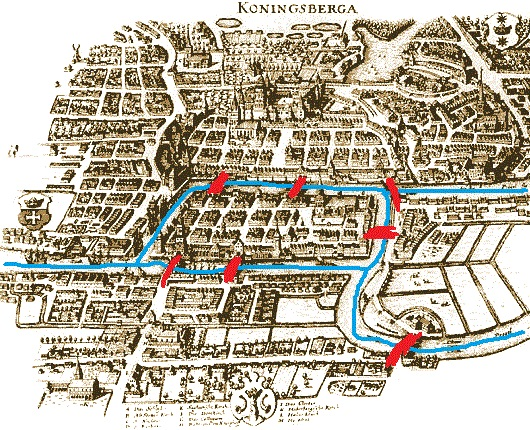
\includegraphics[keepaspectratio]{../images/fig_koenigsberg_aa.jpg}}
\end{column}
\end{columns}
\end{frame}

\begin{frame}{Abstracción topológica de Euler}
\phantomsection\label{abstracciuxf3n-topoluxf3gica-de-euler}
\begin{columns}[T]
\begin{column}{0.5\linewidth}
\pandocbounded{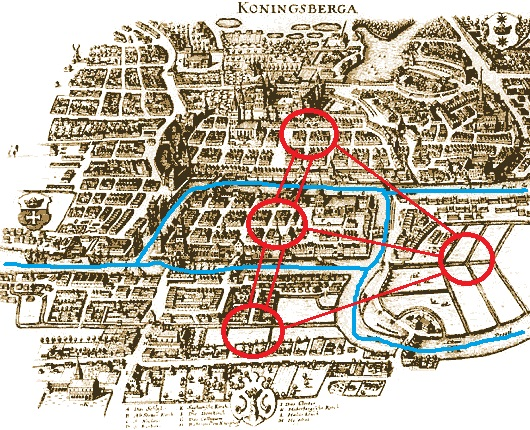
\includegraphics[keepaspectratio]{../images/fig_koenigsberg_aaa.jpg}}
\end{column}

\begin{column}{0.5\linewidth}
\pandocbounded{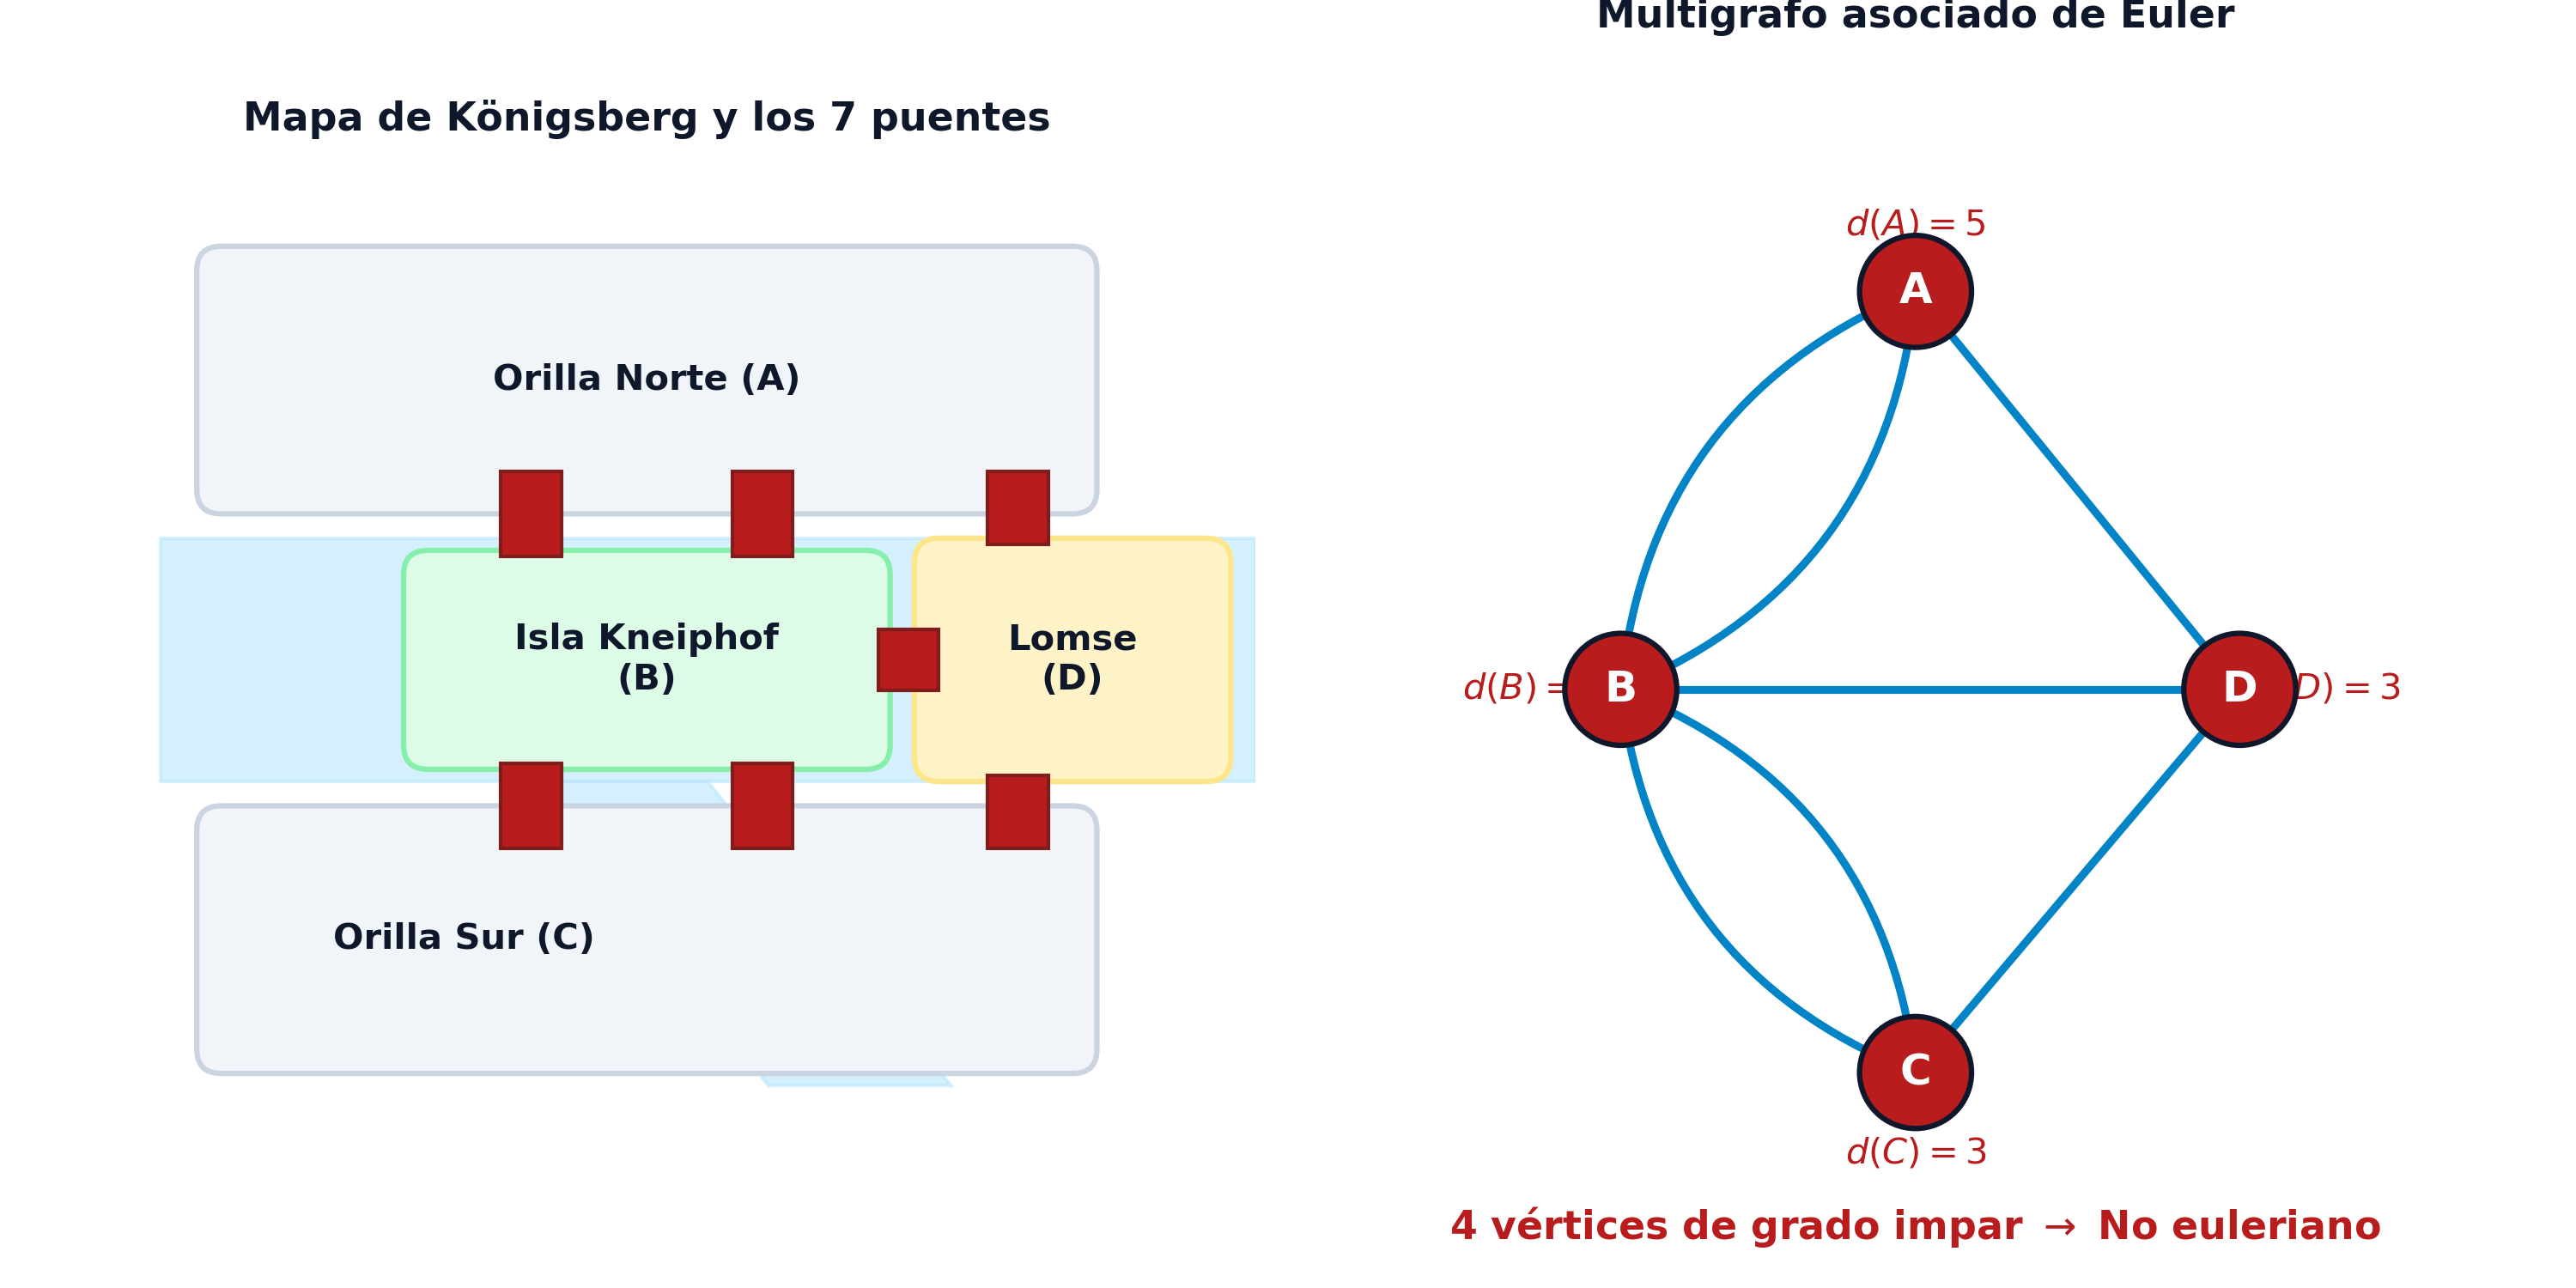
\includegraphics[keepaspectratio]{../images/puentes_konigsberg_grafo.png}}
\end{column}
\end{columns}
\end{frame}

\begin{frame}{Imposibilidad del recorrido en Königsberg}
\phantomsection\label{imposibilidad-del-recorrido-en-kuxf6nigsberg}
\begin{columns}[T]
\begin{column}{0.55\linewidth}
\begin{itemize}
\tightlist
\item
  \textbf{Grado de un nodo}: Aristas incidentes en una masa de tierra.
\item
  \textbf{Condición de tránsito}: Para no repetir puentes, todo nodo
  intermedio requiere grado \textbf{par}.
\item
  \textbf{Grados en Königsberg}: \(d(A)=5\), \(d(B)=3\), \(d(C)=3\),
  \(d(D)=3\) (todos impares).
\item
  \textbf{Conclusión}: Al tener 4 nodos impares, el circuito euleriano
  es \textbf{imposible}.
\end{itemize}
\end{column}

\begin{column}{0.45\linewidth}
\begin{tcolorbox}[enhanced jigsaw, toptitle=1mm, opacityback=0, opacitybacktitle=0.6, colback=white, arc=.35mm, bottomrule=.15mm, titlerule=0mm, coltitle=black, breakable, bottomtitle=1mm, left=2mm, title=\textcolor{quarto-callout-important-color}{\faExclamation}\hspace{0.5em}{Principio de Euler}, colbacktitle=quarto-callout-important-color!10!white, rightrule=.15mm, toprule=.15mm, colframe=quarto-callout-important-color-frame, leftrule=.75mm]

Un grafo conexo admite un circuito euleriano s.i.s. \textbf{todos sus
vértices tienen grado par}.

\end{tcolorbox}
\end{column}
\end{columns}
\end{frame}

\section{Conceptos fundamentales}\label{conceptos-fundamentales}

\begin{frame}{Definición formal de grafos no dirigidos y digrafos}
\phantomsection\label{definiciuxf3n-formal-de-grafos-no-dirigidos-y-digrafos}
\begin{columns}[T]
\begin{column}{0.5\linewidth}
\begin{tcolorbox}[enhanced jigsaw, toptitle=1mm, opacityback=0, opacitybacktitle=0.6, colback=white, arc=.35mm, bottomrule=.15mm, titlerule=0mm, coltitle=black, breakable, bottomtitle=1mm, left=2mm, title=\textcolor{quarto-callout-note-color}{\faInfo}\hspace{0.5em}{Definición: Grafo no dirigido}, colbacktitle=quarto-callout-note-color!10!white, rightrule=.15mm, toprule=.15mm, colframe=quarto-callout-note-color-frame, leftrule=.75mm]

Un \textbf{grafo no dirigido} \(G = (V, E)\) consiste en un conjunto
finito no vacío de \textbf{vértices} \(V\) y un conjunto \(E\) de
\textbf{aristas} formadas por pares no ordenados \(\{u, v\}\) con
\(u, v \in V\).

\end{tcolorbox}
\end{column}

\begin{column}{0.5\linewidth}
\begin{tcolorbox}[enhanced jigsaw, toptitle=1mm, opacityback=0, opacitybacktitle=0.6, colback=white, arc=.35mm, bottomrule=.15mm, titlerule=0mm, coltitle=black, breakable, bottomtitle=1mm, left=2mm, title=\textcolor{quarto-callout-note-color}{\faInfo}\hspace{0.5em}{Definición: Grafo dirigido (Digrafo)}, colbacktitle=quarto-callout-note-color!10!white, rightrule=.15mm, toprule=.15mm, colframe=quarto-callout-note-color-frame, leftrule=.75mm]

Un \textbf{digrafo} \(G = (V, U)\) consiste en un conjunto de vértices
\(V\) y un conjunto \(U\) de \textbf{arcos} formados por tuplas
ordenadas \((u, v)\) donde \(u\) es el nodo origen y \(v\) el nodo
destino.

\end{tcolorbox}
\end{column}
\end{columns}
\end{frame}

\begin{frame}{Ejemplo: Red de transporte aéreo}
\phantomsection\label{ejemplo-red-de-transporte-auxe9reo}
\begin{columns}[T]
\begin{column}{0.55\linewidth}
\begin{itemize}
\tightlist
\item
  \textbf{Modelado de infraestructuras}: Los nodos representan
  aeropuertos y los arcos representan vuelos directos de ida sin escala.
\item
  \textbf{Nodos de la red}: Aeropuertos
  \(V = \{\text{MAD}, \text{BCN}, \text{PAR}, \text{LON}\}\).
\item
  \textbf{Arcos antiparalelos}: \((\text{PAR}, \text{BCN})\) y
  \((\text{BCN}, \text{PAR})\) permiten tránsito bidireccional.
\end{itemize}
\end{column}

\begin{column}{0.45\linewidth}
\pandocbounded{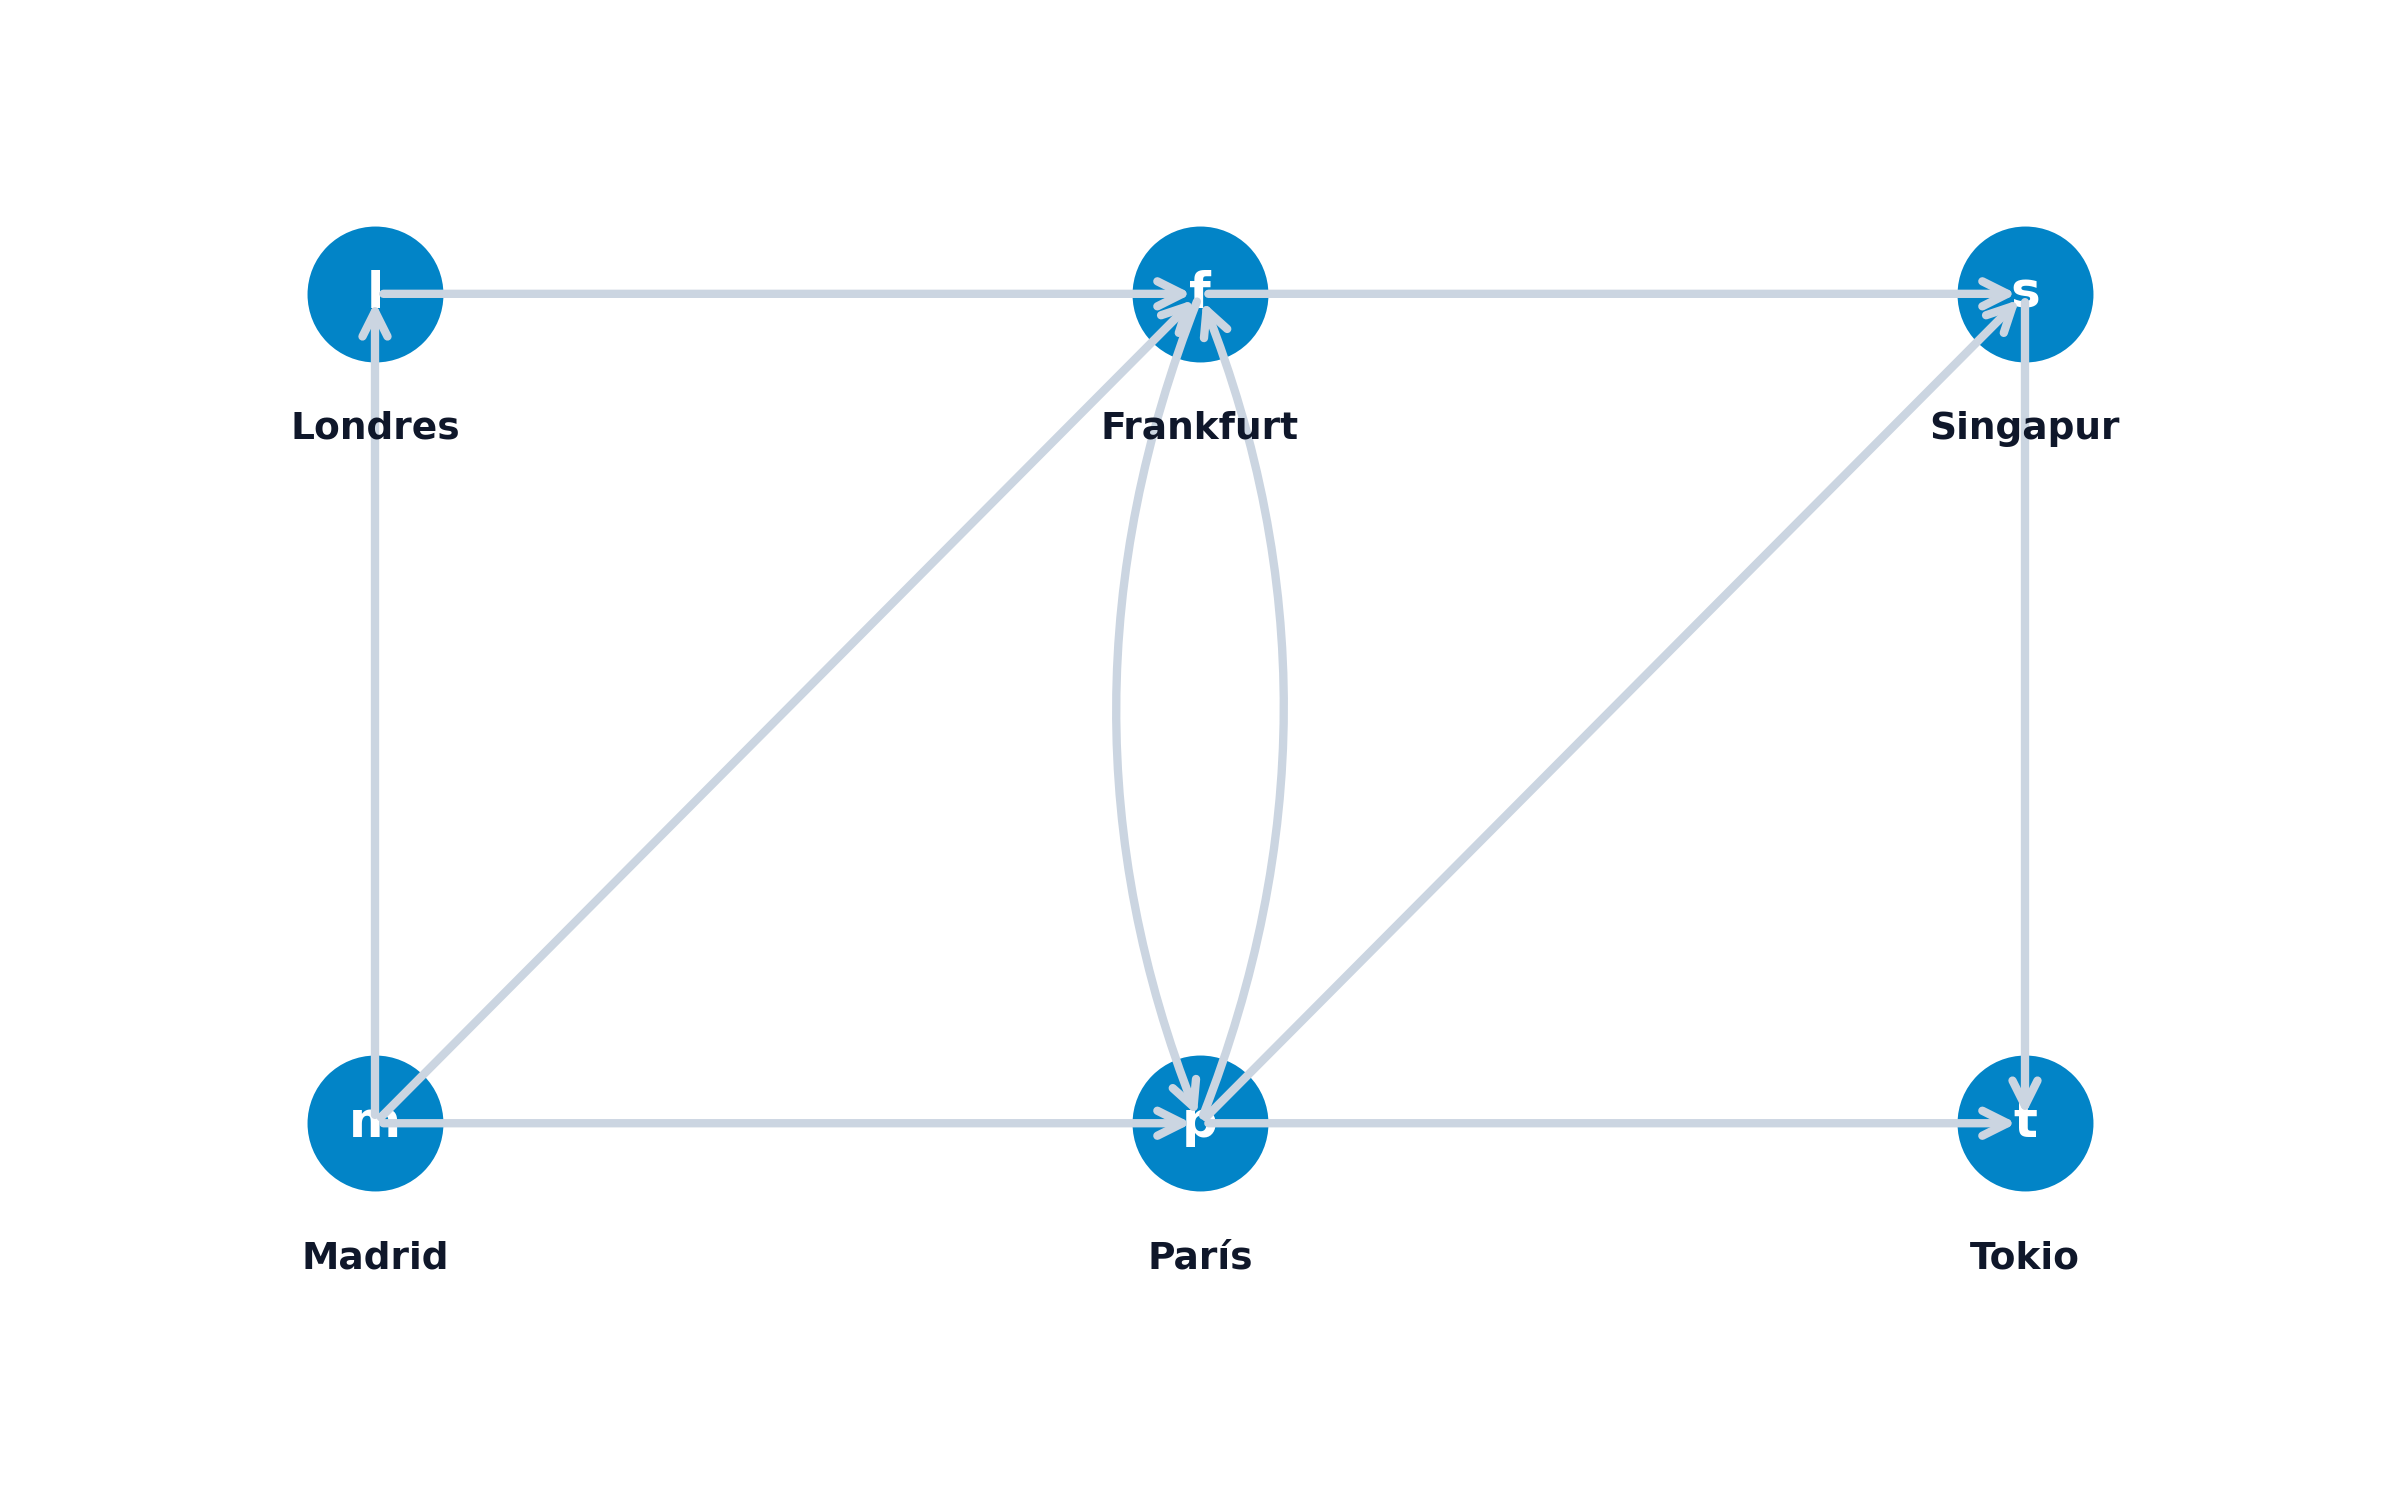
\includegraphics[keepaspectratio]{../images/red_vuelos_ejemplo.png}}
\end{column}
\end{columns}
\end{frame}

\begin{frame}{Estructura abstracta de digrafos}
\phantomsection\label{estructura-abstracta-de-digrafos}
\begin{columns}[T]
\begin{column}{0.55\linewidth}
\begin{itemize}
\tightlist
\item
  \textbf{Tipología de arcos orientados}:

  \begin{itemize}
  \tightlist
  \item
    \textbf{Bucles (autodirecciones)}: \((2, 2)\) en el nodo 2.
  \item
    \textbf{Arcos antiparalelos}: Par de arcos en sentidos opuestos,
    como \((1, 2)\) y \((2, 1)\) o \((2, 4)\) y \((4, 2)\).
  \item
    \textbf{Arcos simples}: Arcos dirigidos en un único sentido, como
    \((1, 3)\), \((2, 3)\) y \((3, 4)\).
  \end{itemize}
\end{itemize}
\end{column}

\begin{column}{0.45\linewidth}
\pandocbounded{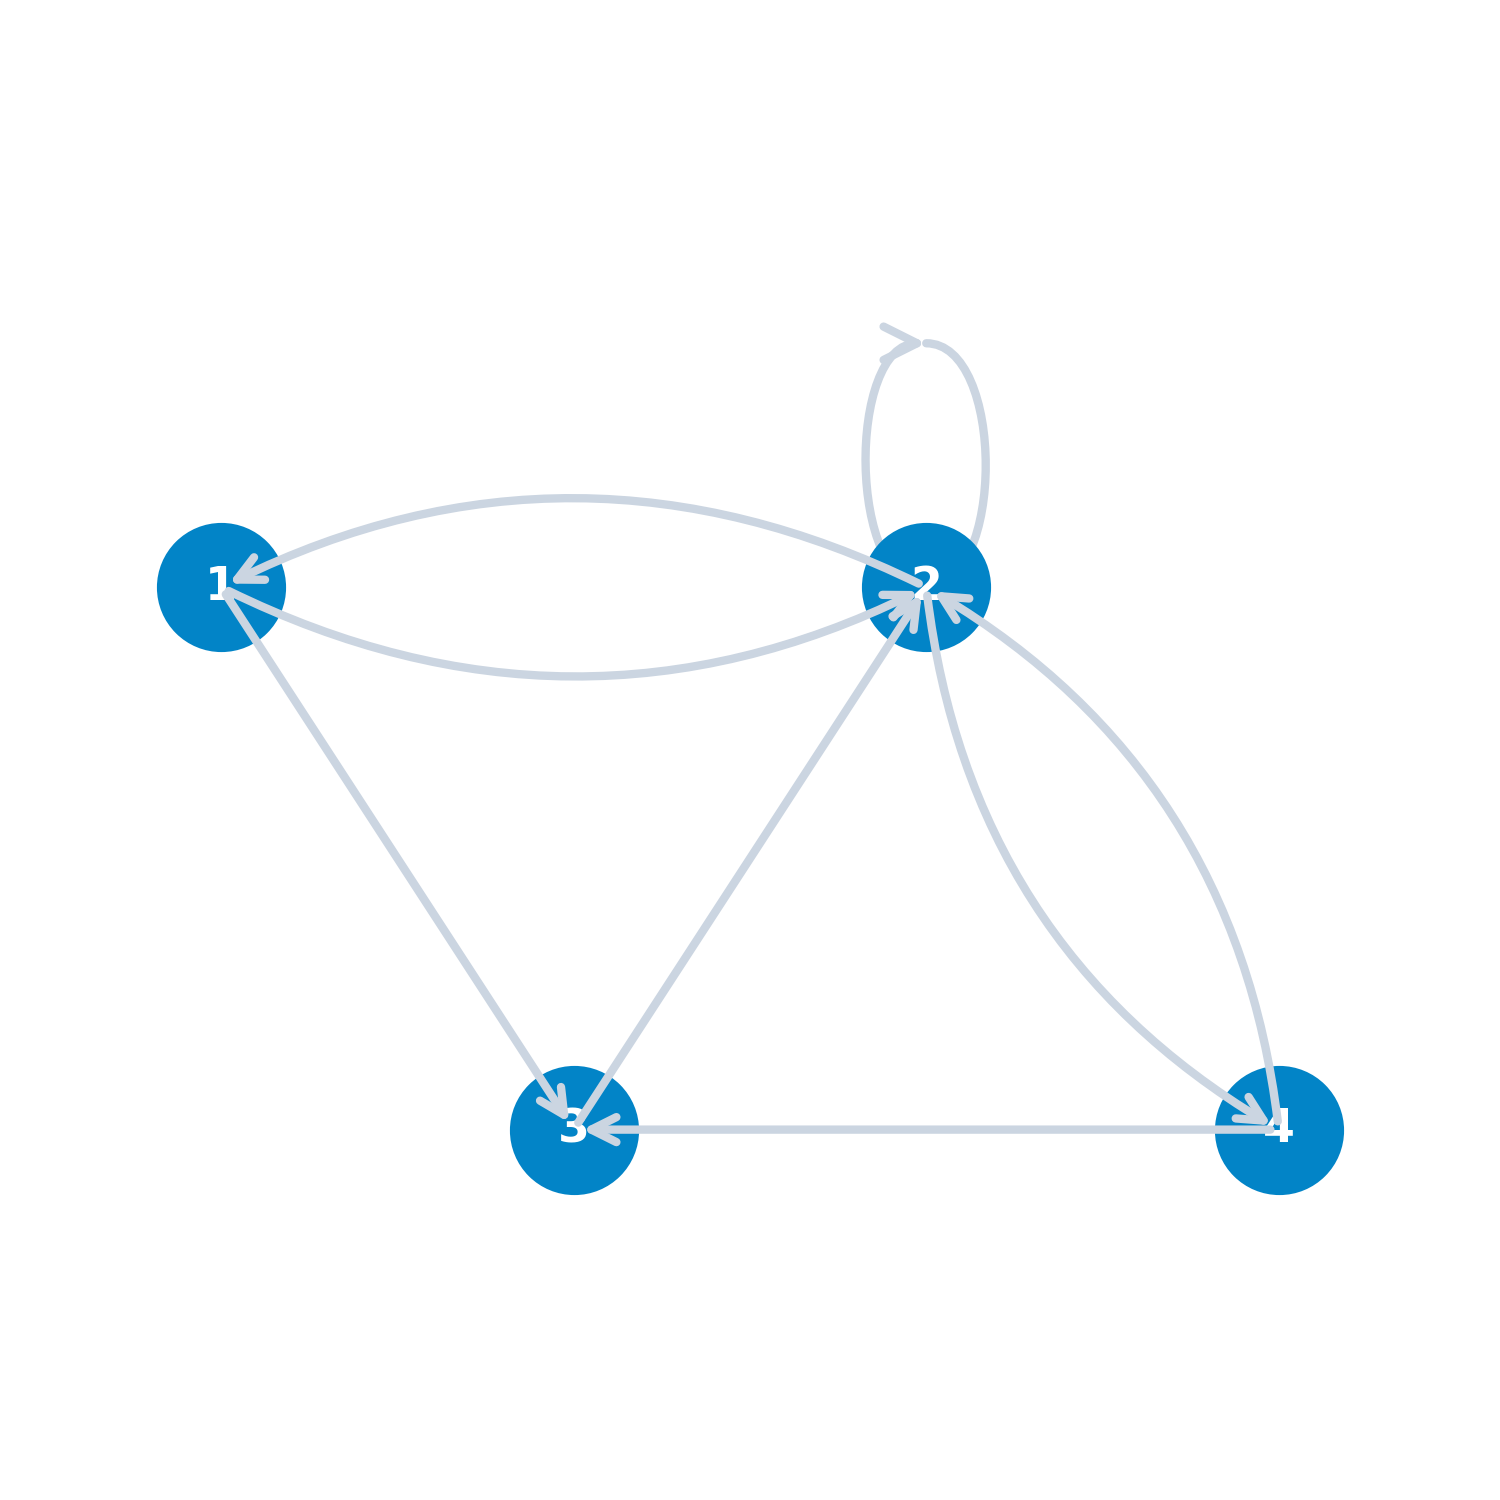
\includegraphics[keepaspectratio]{../images/digrafo_definicion.png}}
\end{column}
\end{columns}
\end{frame}

\begin{frame}{Adyacencia y vecindades de un nodo}
\phantomsection\label{adyacencia-y-vecindades-de-un-nodo}
\begin{tcolorbox}[enhanced jigsaw, toptitle=1mm, opacityback=0, opacitybacktitle=0.6, colback=white, arc=.35mm, bottomrule=.15mm, titlerule=0mm, coltitle=black, breakable, bottomtitle=1mm, left=2mm, title=\textcolor{quarto-callout-note-color}{\faInfo}\hspace{0.5em}{Definición: Adyacencia y vecindades}, colbacktitle=quarto-callout-note-color!10!white, rightrule=.15mm, toprule=.15mm, colframe=quarto-callout-note-color-frame, leftrule=.75mm]

Dado un digrafo \(G = (V, U)\) o grafo no dirigido \(G = (V, E)\) y un
nodo \(i \in V\):

\begin{itemize}
\tightlist
\item
  \textbf{Nodos adyacentes}: Dos nodos \(i, j \in V\) son adyacentes si
  existe una conexión directa entre ellos (\((i,j) \in U\) ó
  \((j,i) \in U\)).
\item
  \textbf{Conjunto de Sucesores}:
  \(\Gamma^+(i) = \{j \in V : (i, j) \in U\}\), nodos hacia los que
  parten arcos desde \(i\).
\item
  \textbf{Conjunto de Predecesores}:
  \(\Gamma^-(i) = \{j \in V : (j, i) \in U\}\), nodos desde los que
  llegan arcos a \(i\).
\item
  \textbf{Vecindad Total}: \(\Gamma(i) = \Gamma^+(i) \cup \Gamma^-(i)\),
  conjunto combinado de sucesores y predecesores de \(i\).
\end{itemize}

\end{tcolorbox}
\end{frame}

\begin{frame}{Incidencia de arcos}
\phantomsection\label{incidencia-de-arcos}
\begin{tcolorbox}[enhanced jigsaw, toptitle=1mm, opacityback=0, opacitybacktitle=0.6, colback=white, arc=.35mm, bottomrule=.15mm, titlerule=0mm, coltitle=black, breakable, bottomtitle=1mm, left=2mm, title=\textcolor{quarto-callout-note-color}{\faInfo}\hspace{0.5em}{Definición: Incidencia de arcos}, colbacktitle=quarto-callout-note-color!10!white, rightrule=.15mm, toprule=.15mm, colframe=quarto-callout-note-color-frame, leftrule=.75mm]

Dado un digrafo \(G = (V, U)\) o grafo no dirigido \(G = (V, E)\):

\begin{itemize}
\tightlist
\item
  \textbf{Arcos adyacentes}: Dos arcos \(u_1, u_2 \in U\) son adyacentes
  cuando comparten al menos un nodo extremo común (por ejemplo, los
  arcos \((1, 2)\) y \((2, 4)\) en el nodo \(2\)).
\item
  \textbf{Incidencia de salida}: Un arco \(u = (i, j) \in U\) es
  \textbf{incidente de salida} en su nodo origen \(i\).
\item
  \textbf{Incidencia de entrada}: Un arco \(u = (i, j) \in U\) es
  \textbf{incidente de entrada} en su nodo destino \(j\).
\end{itemize}

\end{tcolorbox}
\end{frame}

\begin{frame}{Semigrados exterior e interior}
\phantomsection\label{semigrados-exterior-e-interior}
\begin{tcolorbox}[enhanced jigsaw, toptitle=1mm, opacityback=0, opacitybacktitle=0.6, colback=white, arc=.35mm, bottomrule=.15mm, titlerule=0mm, coltitle=black, breakable, bottomtitle=1mm, left=2mm, title=\textcolor{quarto-callout-note-color}{\faInfo}\hspace{0.5em}{Definición: Semigrados exterior e interior}, colbacktitle=quarto-callout-note-color!10!white, rightrule=.15mm, toprule=.15mm, colframe=quarto-callout-note-color-frame, leftrule=.75mm]

Dado un digrafo \(G = (V, U)\) y un nodo \(i \in V\):

\begin{itemize}
\item
  \textbf{Semigrado exterior}: \[d^+(i) = |\Gamma^+(i)|\] Número exacto
  de arcos salientes que parten del nodo \(i\).
\item
  \textbf{Semigrado interior}: \[d^-(i) = |\Gamma^-(i)|\] Número exacto
  de arcos entrantes que ingresan en el nodo \(i\).
\end{itemize}

\end{tcolorbox}
\end{frame}

\begin{frame}{Grado total y nodos notables}
\phantomsection\label{grado-total-y-nodos-notables}
\begin{tcolorbox}[enhanced jigsaw, toptitle=1mm, opacityback=0, opacitybacktitle=0.6, colback=white, arc=.35mm, bottomrule=.15mm, titlerule=0mm, coltitle=black, breakable, bottomtitle=1mm, left=2mm, title=\textcolor{quarto-callout-note-color}{\faInfo}\hspace{0.5em}{Definición: Grado total y nodos notables}, colbacktitle=quarto-callout-note-color!10!white, rightrule=.15mm, toprule=.15mm, colframe=quarto-callout-note-color-frame, leftrule=.75mm]

Dado un grafo \(G = (V, E)\) o digrafo \(G = (V, U)\) y un nodo
\(i \in V\):

\begin{itemize}
\tightlist
\item
  \textbf{Grado total}: \[d(i) = d^+(i) + d^-(i)\] Número total de arcos
  o aristas incidentes en el nodo \(i\).
\item
  \textbf{Nodo pendiente o hoja}: Nodo con grado total exactamente igual
  a 1 (\(d(i) = 1\)).
\item
  \textbf{Nodo aislado}: Nodo desprovisto de conexiones incidentes
  (\(d(i) = 0\)).
\end{itemize}

\end{tcolorbox}
\end{frame}

\begin{frame}{Ilustración de vecindades y semigrados}
\phantomsection\label{ilustraciuxf3n-de-vecindades-y-semigrados}
\begin{columns}[T]
\begin{column}{0.5\linewidth}
\begin{itemize}
\tightlist
\item
  \textbf{Vecindad del nodo 3}:

  \begin{itemize}
  \tightlist
  \item
    Sucesores: \(\Gamma^+(3) = \{2\}\)
  \item
    Predecesores: \(\Gamma^-(3) = \{1, 4\}\)
  \item
    Vecindad total: \(\Gamma(3) = \{1, 2, 4\}\)
  \end{itemize}
\end{itemize}
\end{column}

\begin{column}{0.5\linewidth}
\begin{itemize}
\tightlist
\item
  \textbf{Semigrados y Nodos notables}:

  \begin{itemize}
  \tightlist
  \item
    Entrada y salida: \(d^+(3)=1, d^-(3)=2\)
  \item
    Grado total: \(d(3) = 1 + 2 = 3\)
  \item
    Nodo 5: \(d^+(5)=0, d^-(5)=1 \implies d(5)=1\)
  \end{itemize}
\end{itemize}
\end{column}
\end{columns}

\begin{columns}[T]
\begin{column}{0.5\linewidth}
\begin{center}
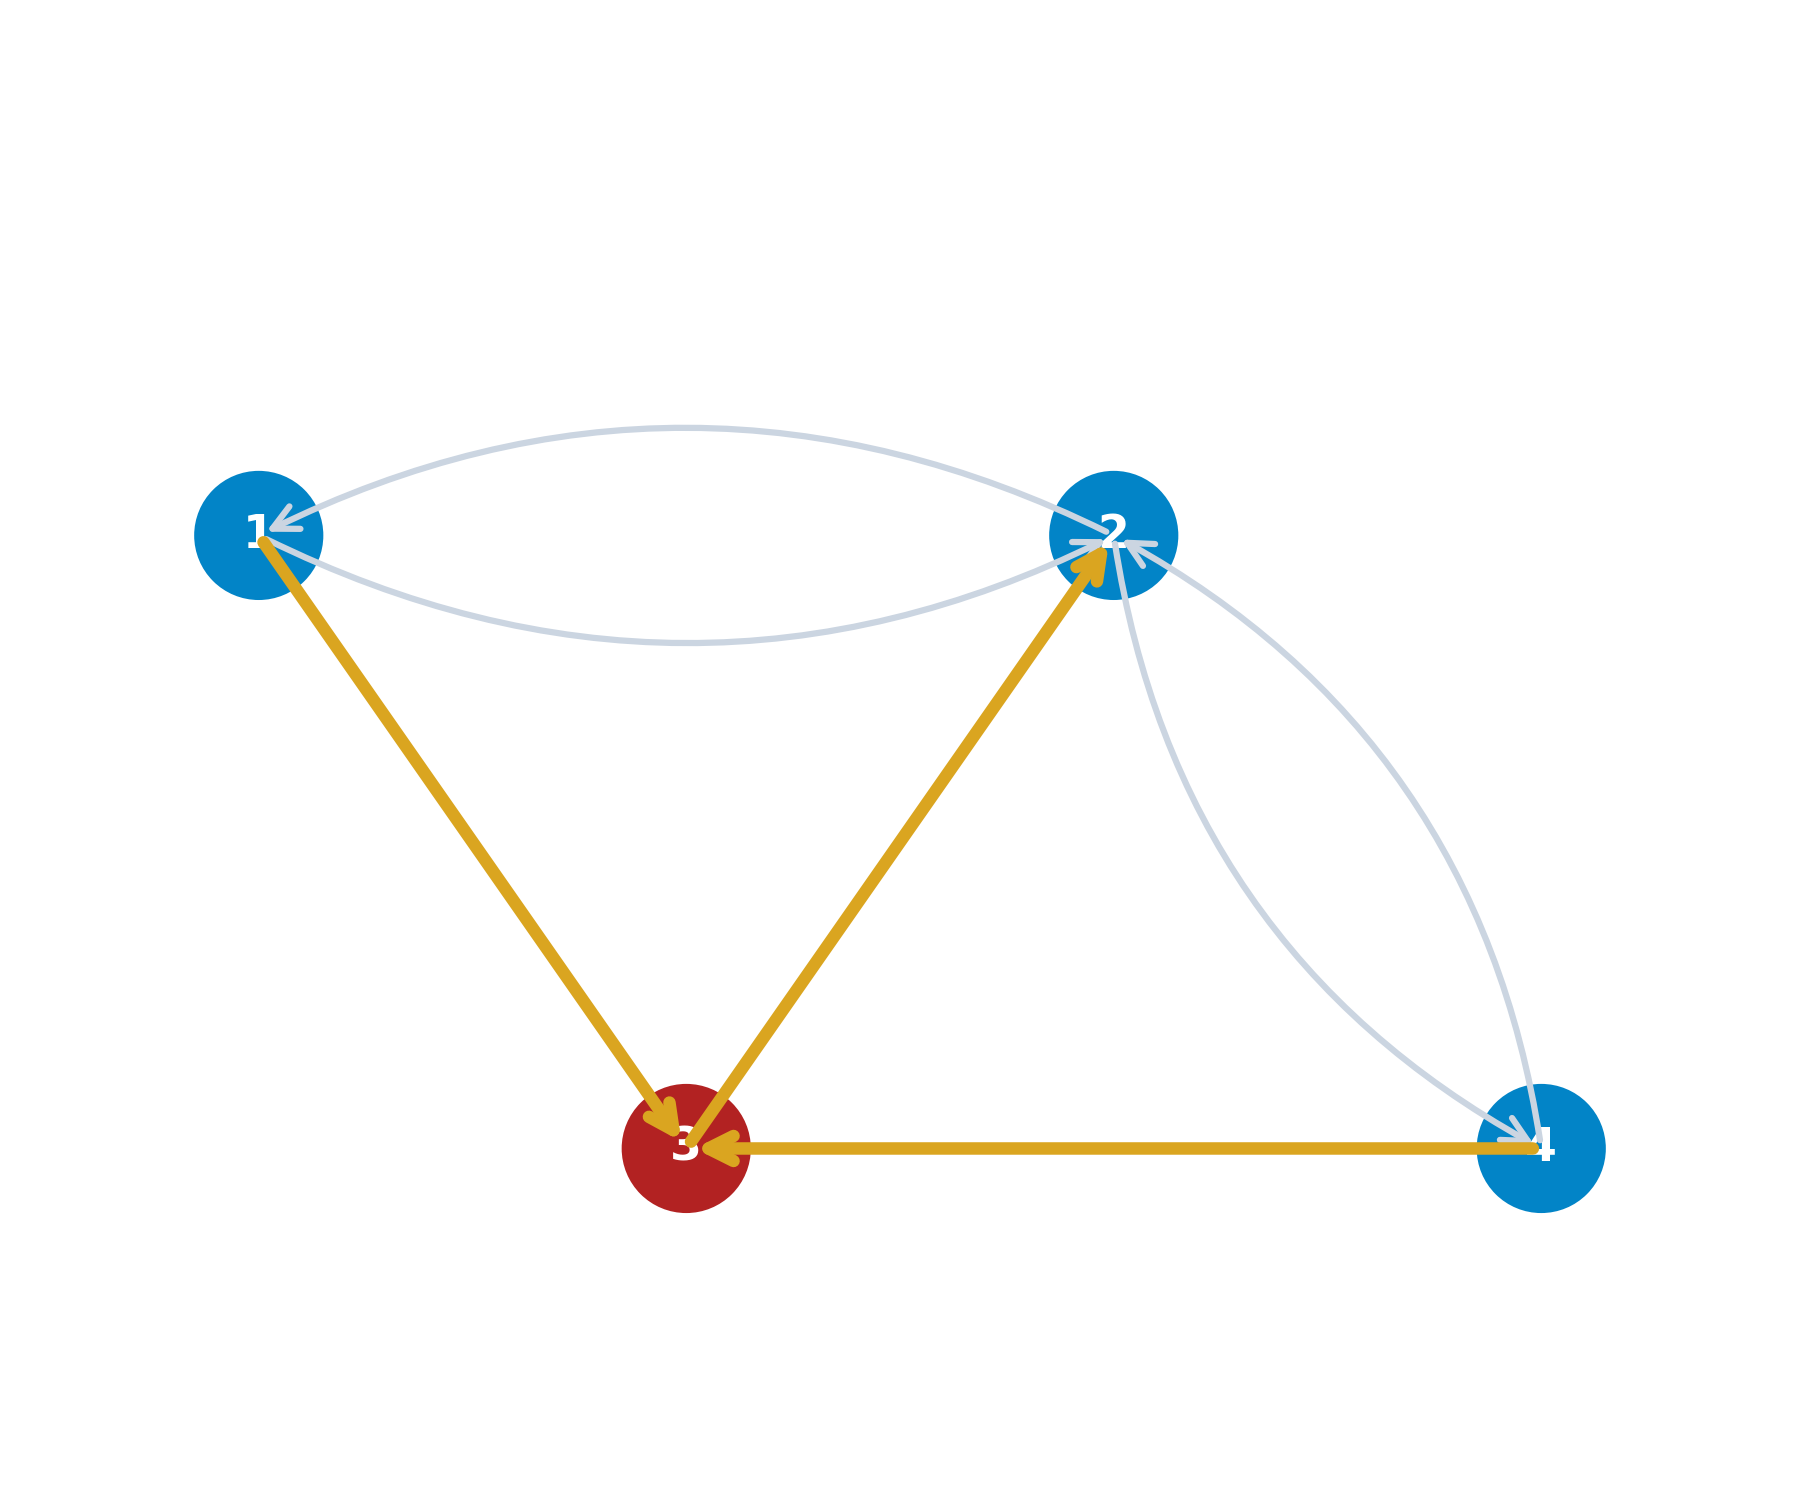
\includegraphics[width=\linewidth,height=2.60417in,keepaspectratio]{../images/adyacencia_vecindades.png}
\end{center}
\end{column}

\begin{column}{0.5\linewidth}
\begin{center}
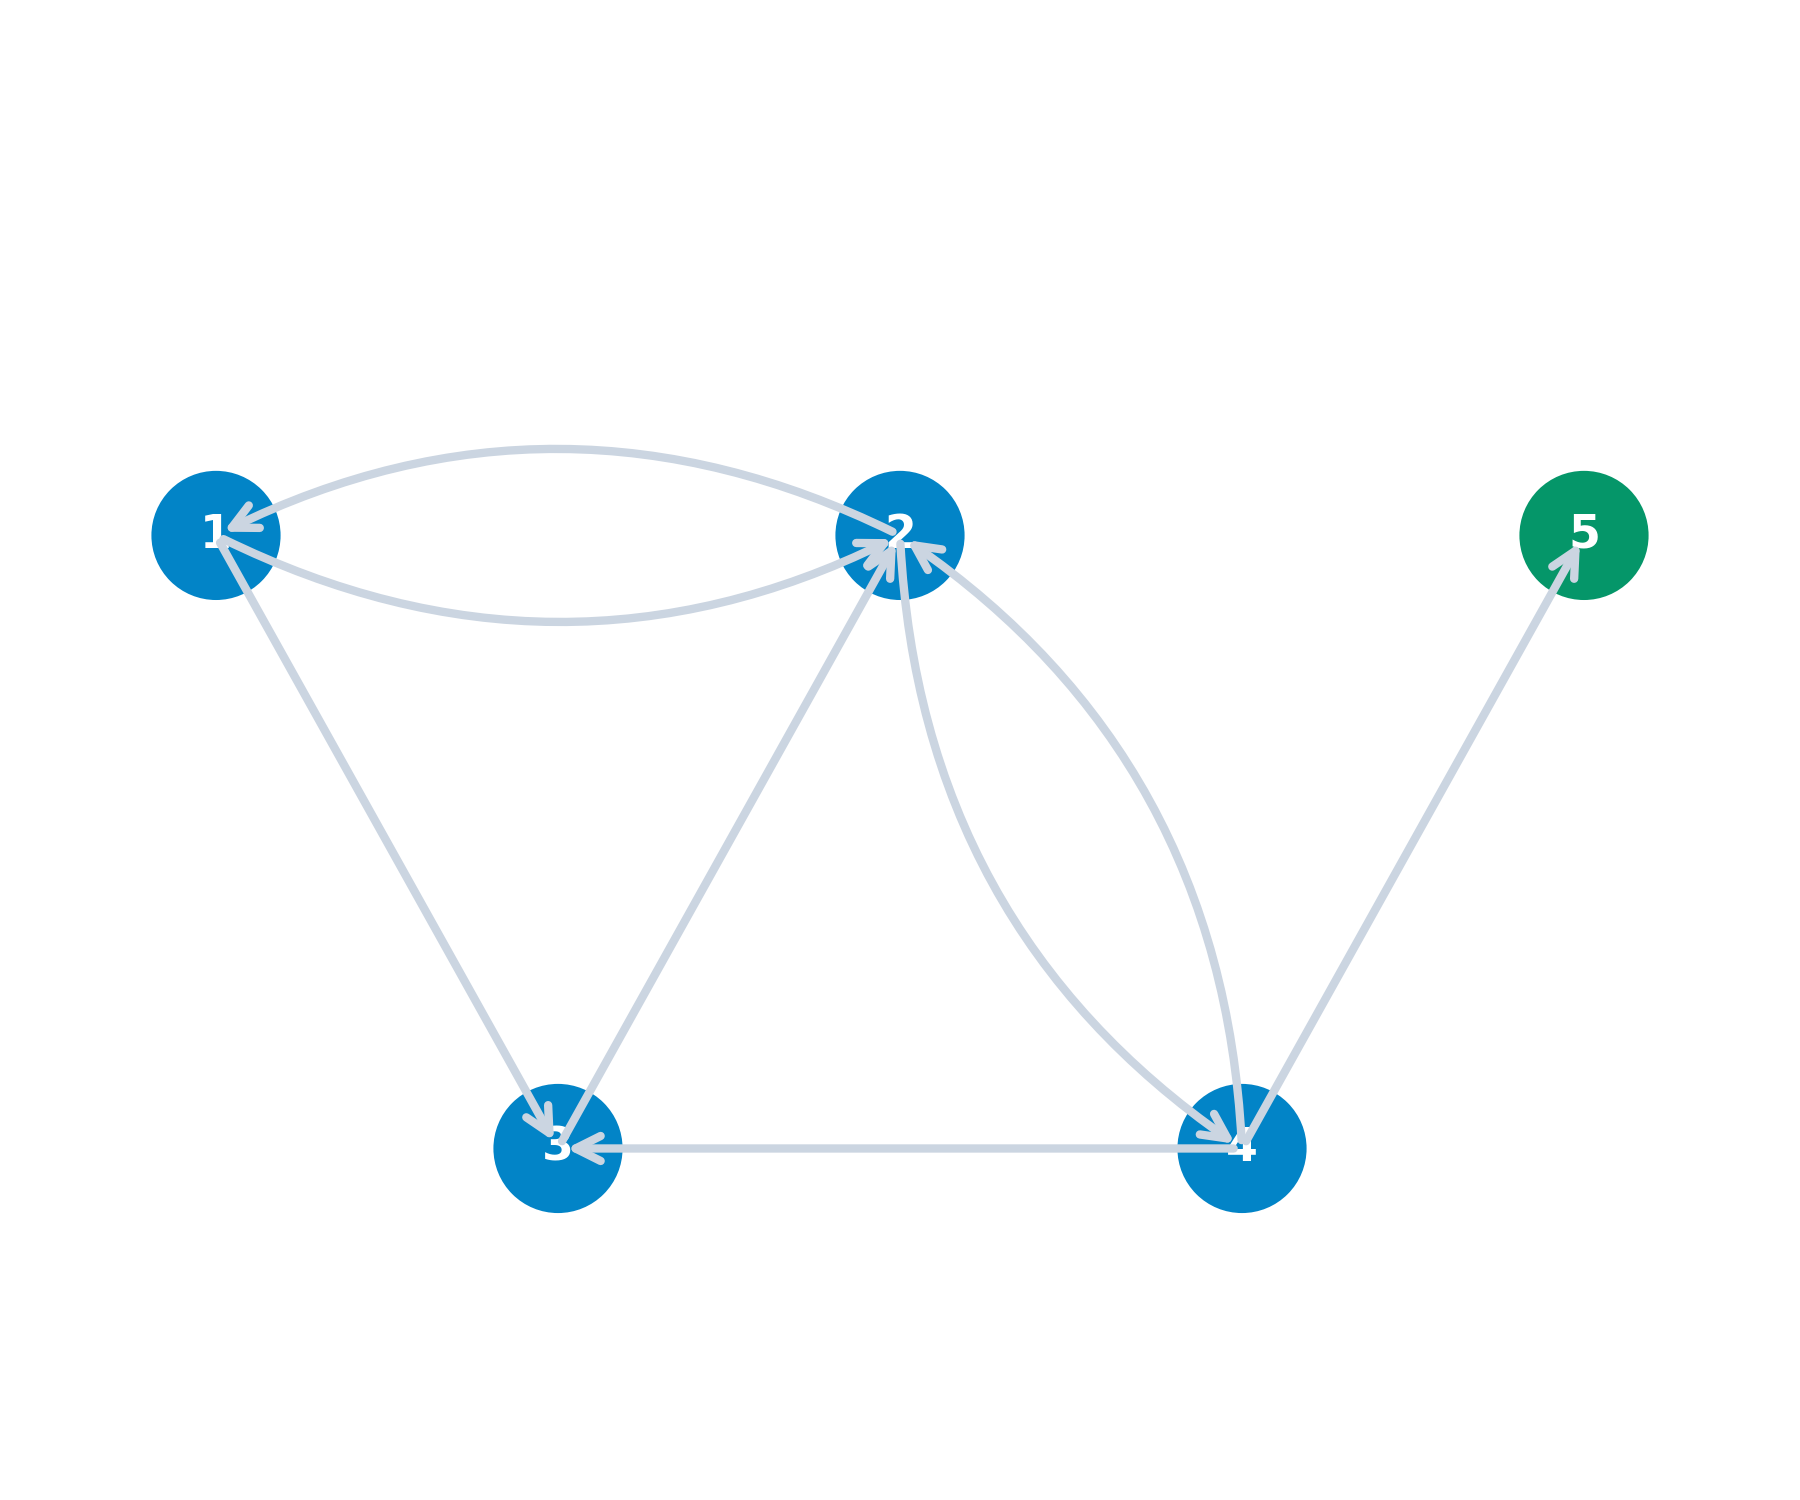
\includegraphics[width=\linewidth,height=2.60417in,keepaspectratio]{../images/grado_nodos.png}
\end{center}
\end{column}
\end{columns}
\end{frame}

\begin{frame}{Lema del apretón de manos (Handshaking Lemma)}
\phantomsection\label{lema-del-apretuxf3n-de-manos-handshaking-lemma}
\begin{columns}[T]
\begin{column}{0.6\linewidth}
\begin{tcolorbox}[enhanced jigsaw, toptitle=1mm, opacityback=0, opacitybacktitle=0.6, colback=white, arc=.35mm, bottomrule=.15mm, titlerule=0mm, coltitle=black, breakable, bottomtitle=1mm, left=2mm, title=\textcolor{quarto-callout-important-color}{\faExclamation}\hspace{0.5em}{Teorema de la suma de grados (Handshaking Lemma)}, colbacktitle=quarto-callout-important-color!10!white, rightrule=.15mm, toprule=.15mm, colframe=quarto-callout-important-color-frame, leftrule=.75mm]

En todo grafo no dirigido \(G = (V, E)\) con \(|V| = n\) vértices y
\(|E| = m\) aristas, la suma de los grados de todos los vértices es
igual al doble del número total de aristas: \[
\sum_{v \in V} d(v) = 2m
\]

\end{tcolorbox}
\end{column}

\begin{column}{0.4\linewidth}
\begin{itemize}
\tightlist
\item
  \textbf{Significado combinatorio}:

  \begin{itemize}
  \tightlist
  \item
    Cada arista no dirigida conecta exactamente dos vértices extremos.
  \item
    Al sumar los grados de todos los nodos, cada arista se contabiliza
    exactamente dos veces (apretón de manos de dos extremos).
  \end{itemize}
\end{itemize}
\end{column}
\end{columns}
\end{frame}

\begin{frame}{Incidencia de conjuntos de nodos y cortes}
\phantomsection\label{incidencia-de-conjuntos-de-nodos-y-cortes}
\begin{tcolorbox}[enhanced jigsaw, toptitle=1mm, opacityback=0, opacitybacktitle=0.6, colback=white, arc=.35mm, bottomrule=.15mm, titlerule=0mm, coltitle=black, breakable, bottomtitle=1mm, left=2mm, title=\textcolor{quarto-callout-note-color}{\faInfo}\hspace{0.5em}{Definición: Incidencia y corte de un conjunto A}, colbacktitle=quarto-callout-note-color!10!white, rightrule=.15mm, toprule=.15mm, colframe=quarto-callout-note-color-frame, leftrule=.75mm]

Dado un digrafo \(G = (V, U)\) y un subconjunto propio de nodos
\(A \subset V\):

\begin{itemize}
\item
  \textbf{Incidencia Exterior \(w^+(A)\)}: Conjunto de arcos que parten
  de \(A\) y finalizan fuera de \(A\):\\
  \(w^+(A) = \{(i, j) \in U : i \in A, \, j \in V \setminus A\}\)
\item
  \textbf{Incidencia Interior \(w^-(A)\)}: Conjunto de arcos que parten
  de fuera de \(A\) e ingresan en \(A\):\\
  \(w^-(A) = \{(i, j) \in U : i \in V \setminus A, \, j \in A\}\)
\item
  \textbf{Corte \(w(A)\)}: Unión de las incidencias exterior e interior
  de la frontera:\\
  \(w(A) = w^+(A) \cup w^-(A)\)
\end{itemize}

\end{tcolorbox}
\end{frame}

\begin{frame}{Ejemplo: Corte e incidencias para A = \{2, 3\}}
\phantomsection\label{ejemplo-corte-e-incidencias-para-a-2-3}
\begin{columns}[T]
\begin{column}{0.55\linewidth}
Para el subconjunto de nodos \(A = \{2, 3\}\):

\begin{itemize}
\tightlist
\item
  \textbf{Incidencia exterior} (salientes de \(A\)):
  \[\textcolor{firebrick}{w^+(A) = \{(2,4), (3,1), (3,5)\}}\]
\item
  \textbf{Incidencia interior} (entrantes a \(A\)):
  \[\textcolor{dodgerblue}{w^-(A) = \{(1,2), (4,3)\}}\]
\item
  \textbf{Corte total} (frontera cruzada): \[
  \begin{aligned}
  w(A) = \{ &\textcolor{dodgerblue}{(1,2)}, \textcolor{firebrick}{(2,4)}, \textcolor{firebrick}{(3,1)}, \\
            &\textcolor{firebrick}{(3,5)}, \textcolor{dodgerblue}{(4,3)} \}
  \end{aligned}
  \]
\end{itemize}
\end{column}

\begin{column}{0.45\linewidth}
\pandocbounded{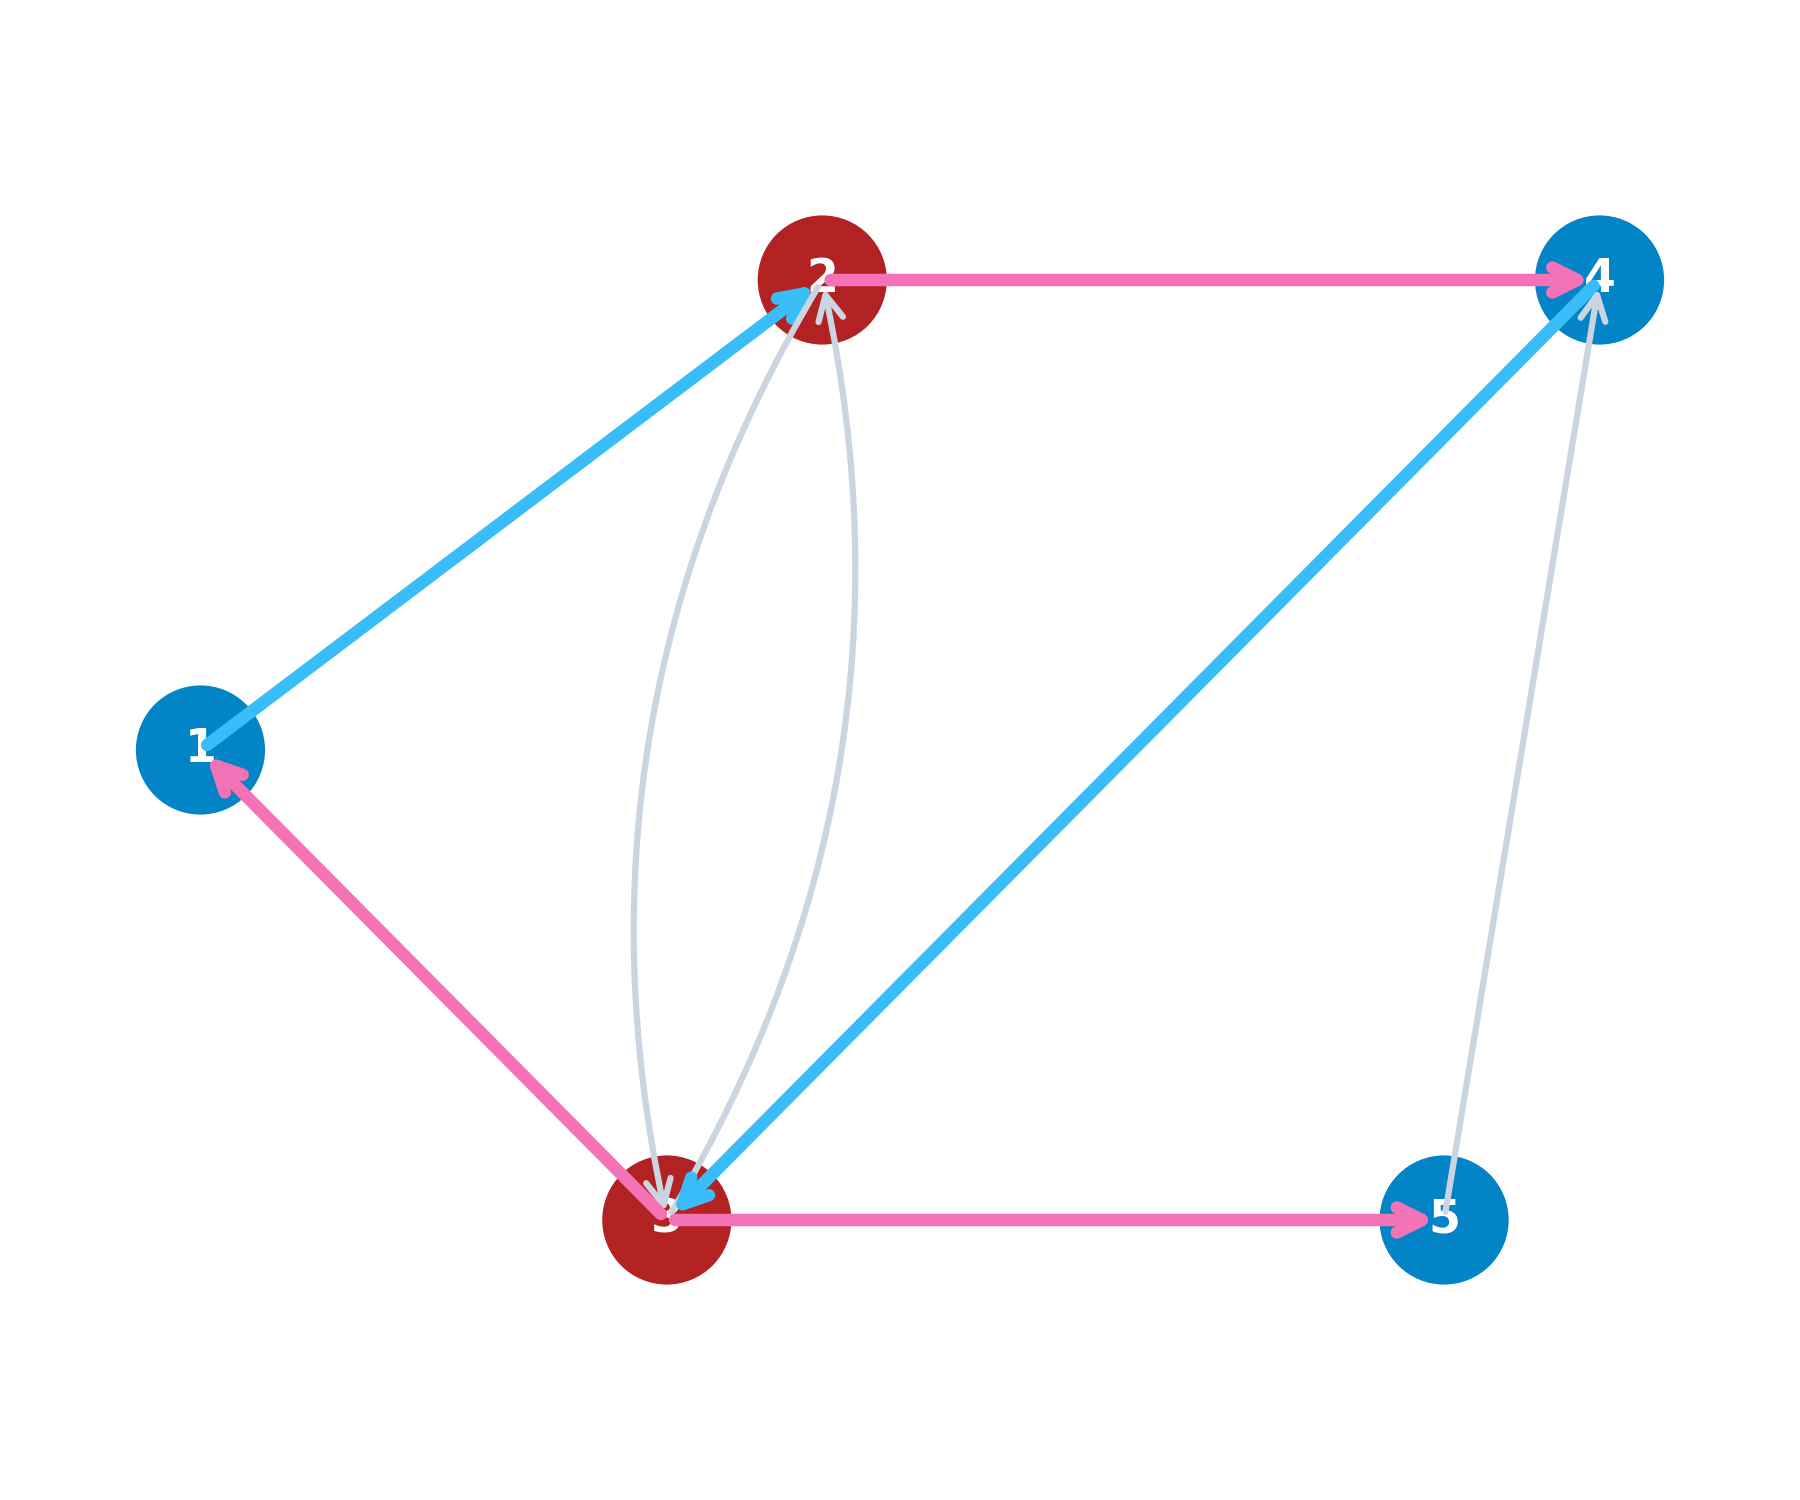
\includegraphics[keepaspectratio]{../images/incidencia_corte_conjuntos.png}}
\end{column}
\end{columns}
\end{frame}

\begin{frame}{Multigrafos y p-grafos}
\phantomsection\label{multigrafos-y-p-grafos}
\begin{columns}[T]
\begin{column}{0.55\linewidth}
\begin{tcolorbox}[enhanced jigsaw, toptitle=1mm, opacityback=0, opacitybacktitle=0.6, colback=white, arc=.35mm, bottomrule=.15mm, titlerule=0mm, coltitle=black, breakable, bottomtitle=1mm, left=2mm, title=\textcolor{quarto-callout-note-color}{\faInfo}\hspace{0.5em}{Definición: Multigrafo y p-grafo}, colbacktitle=quarto-callout-note-color!10!white, rightrule=.15mm, toprule=.15mm, colframe=quarto-callout-note-color-frame, leftrule=.75mm]

\begin{itemize}
\tightlist
\item
  \textbf{Multigrafo / Multidigrafo}: Admite múltiples conexiones o
  aristas en paralelo entre un mismo par de vértices.
\item
  \textbf{Multiplicidad}: Número exacto de conexiones paralelas entre
  dos nodos.
\item
  \textbf{\(p\)-Grafo}: Multigrafo en el que la máxima multiplicidad de
  cualquier par de nodos es \(p\).
\end{itemize}

\end{tcolorbox}
\end{column}

\begin{column}{0.45\linewidth}
\pandocbounded{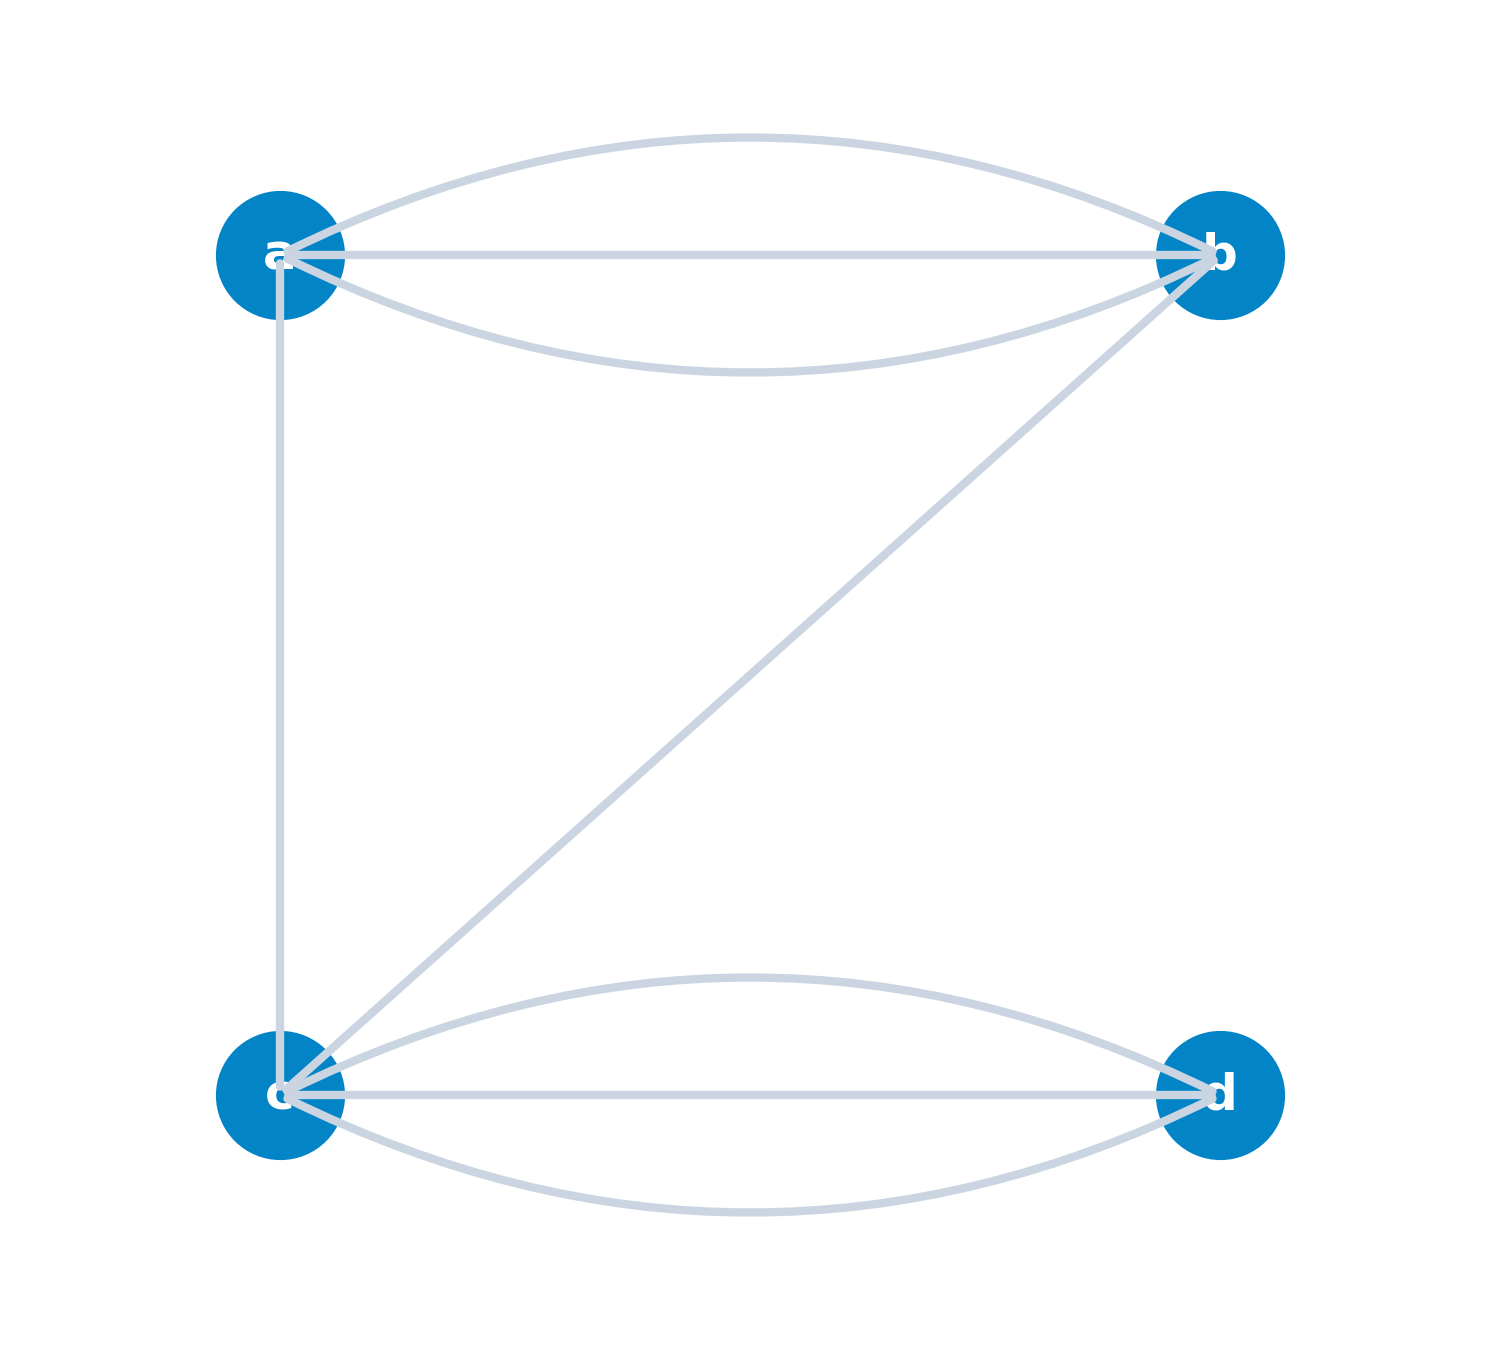
\includegraphics[keepaspectratio]{../images/multigrafos_pgrafos.png}}
\end{column}
\end{columns}
\end{frame}

\begin{frame}{Grafos simples}
\phantomsection\label{grafos-simples}
\begin{tcolorbox}[enhanced jigsaw, toptitle=1mm, opacityback=0, opacitybacktitle=0.6, colback=white, arc=.35mm, bottomrule=.15mm, titlerule=0mm, coltitle=black, breakable, bottomtitle=1mm, left=2mm, title=\textcolor{quarto-callout-note-color}{\faInfo}\hspace{0.5em}{Definición: Grafo simple}, colbacktitle=quarto-callout-note-color!10!white, rightrule=.15mm, toprule=.15mm, colframe=quarto-callout-note-color-frame, leftrule=.75mm]

Un \textbf{grafo simple} (o \textbf{digrafo simple}) es un grafo de
multiplicidad 1 desprovisto de autodirecciones o bucles \((i, i)\).

\begin{itemize}
\tightlist
\item
  \textbf{Propiedad de exclusión}:

  \begin{itemize}
  \tightlist
  \item
    Para cualquier par de vértices \(i, j \in V\), existe como máximo
    una única arista \(\{i, j\} \in E\) (o un único arco
    \((i, j) \in U\)).
  \item
    Ningún nodo está conectado consigo mismo mediante un bucle
    \((i, i) \notin U\).
  \end{itemize}
\end{itemize}

\end{tcolorbox}
\end{frame}

\begin{frame}{Grafos completos (no dirigidos) y Clanes (\(K_n\))}
\phantomsection\label{grafos-completos-no-dirigidos-y-clanes-k_n}
\begin{columns}[T]
\begin{column}{0.55\linewidth}
\begin{tcolorbox}[enhanced jigsaw, toptitle=1mm, opacityback=0, opacitybacktitle=0.6, colback=white, arc=.35mm, bottomrule=.15mm, titlerule=0mm, coltitle=black, breakable, bottomtitle=1mm, left=2mm, title=\textcolor{quarto-callout-note-color}{\faInfo}\hspace{0.5em}{Definición: Grafo completo y Clan Kn}, colbacktitle=quarto-callout-note-color!10!white, rightrule=.15mm, toprule=.15mm, colframe=quarto-callout-note-color-frame, leftrule=.75mm]

Un \textbf{grafo completo} \(G = (V, E)\) (o \textbf{clan / clique}
\(K_n\)) es un grafo simple no dirigido en el que todo par de vértices
distintos se encuentra directamente conectado por una arista: \[
\{i, j\} \in E, \quad \forall i \neq j \in V
\]

\end{tcolorbox}

\begin{itemize}
\tightlist
\item
  \textbf{Número total de aristas}:
  \(m = \binom{n}{2} = \frac{n(n-1)}{2}\).
\end{itemize}
\end{column}

\begin{column}{0.45\linewidth}
\begin{columns}[T]
\begin{column}{0.5\linewidth}
\begin{center}
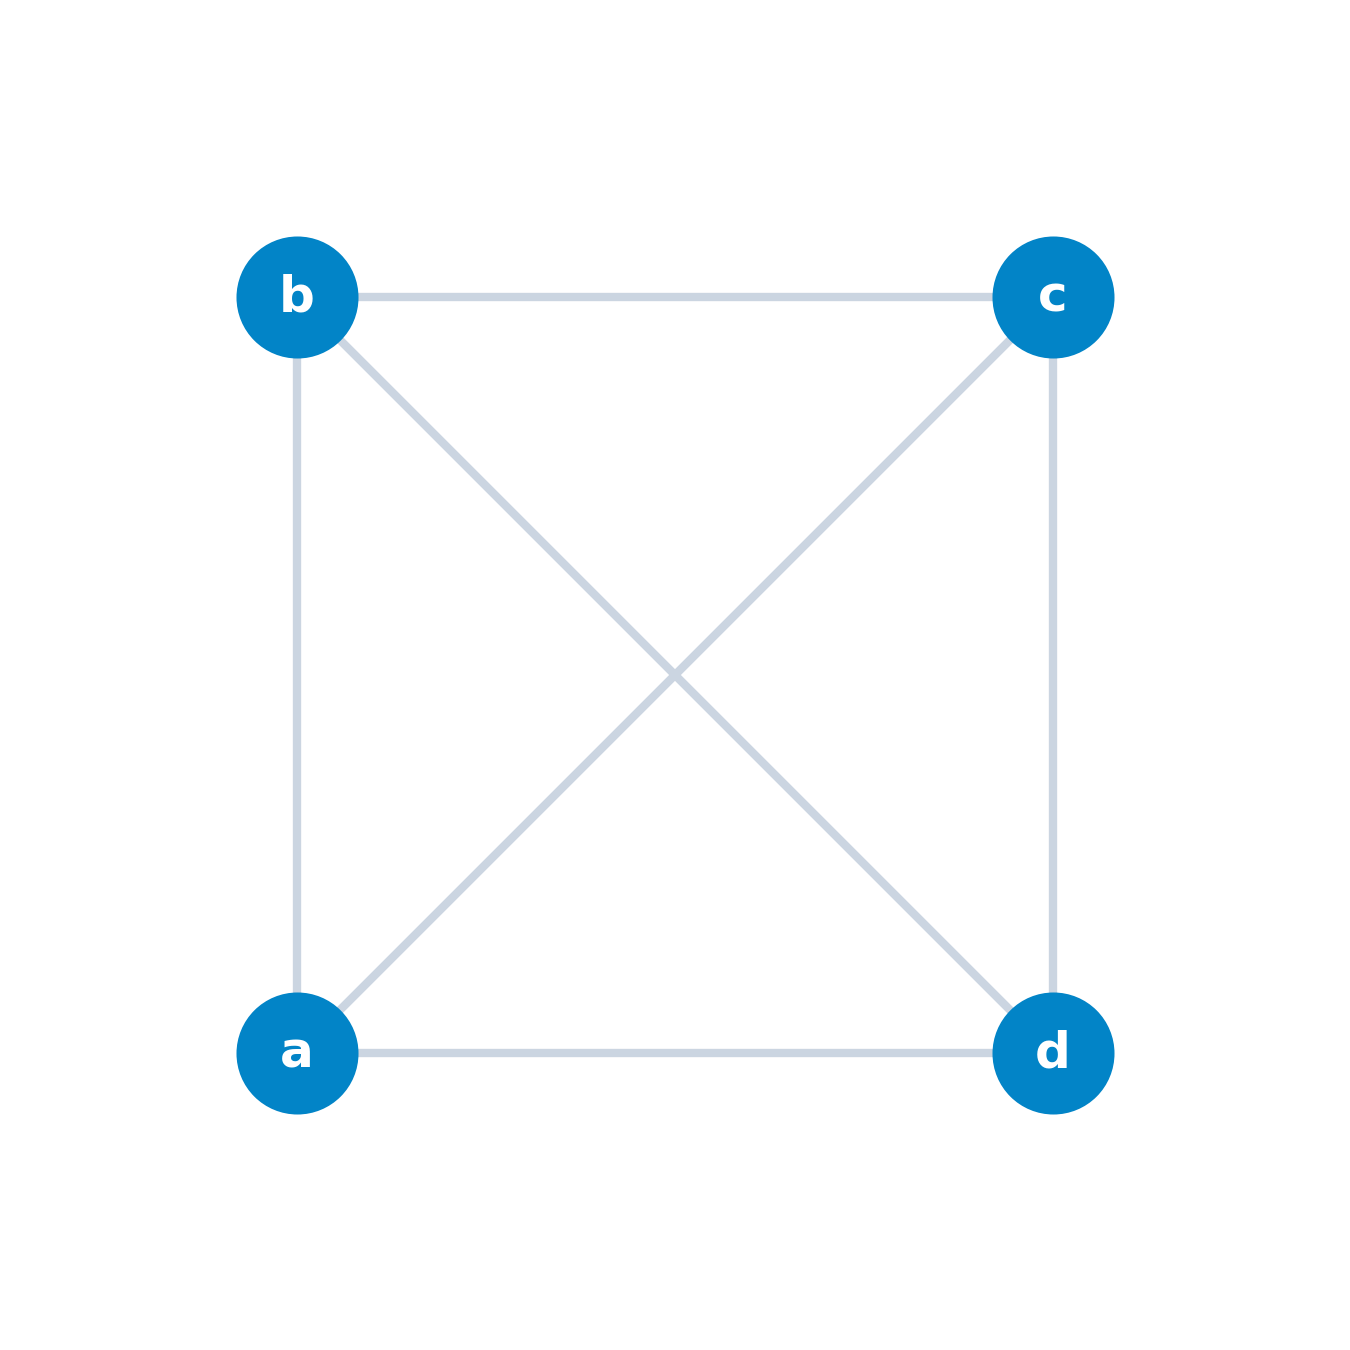
\includegraphics[width=0.9\linewidth,height=\textheight,keepaspectratio]{../images/clan_k4_ejemplo.png}
\end{center}
\end{column}

\begin{column}{0.5\linewidth}
\begin{center}
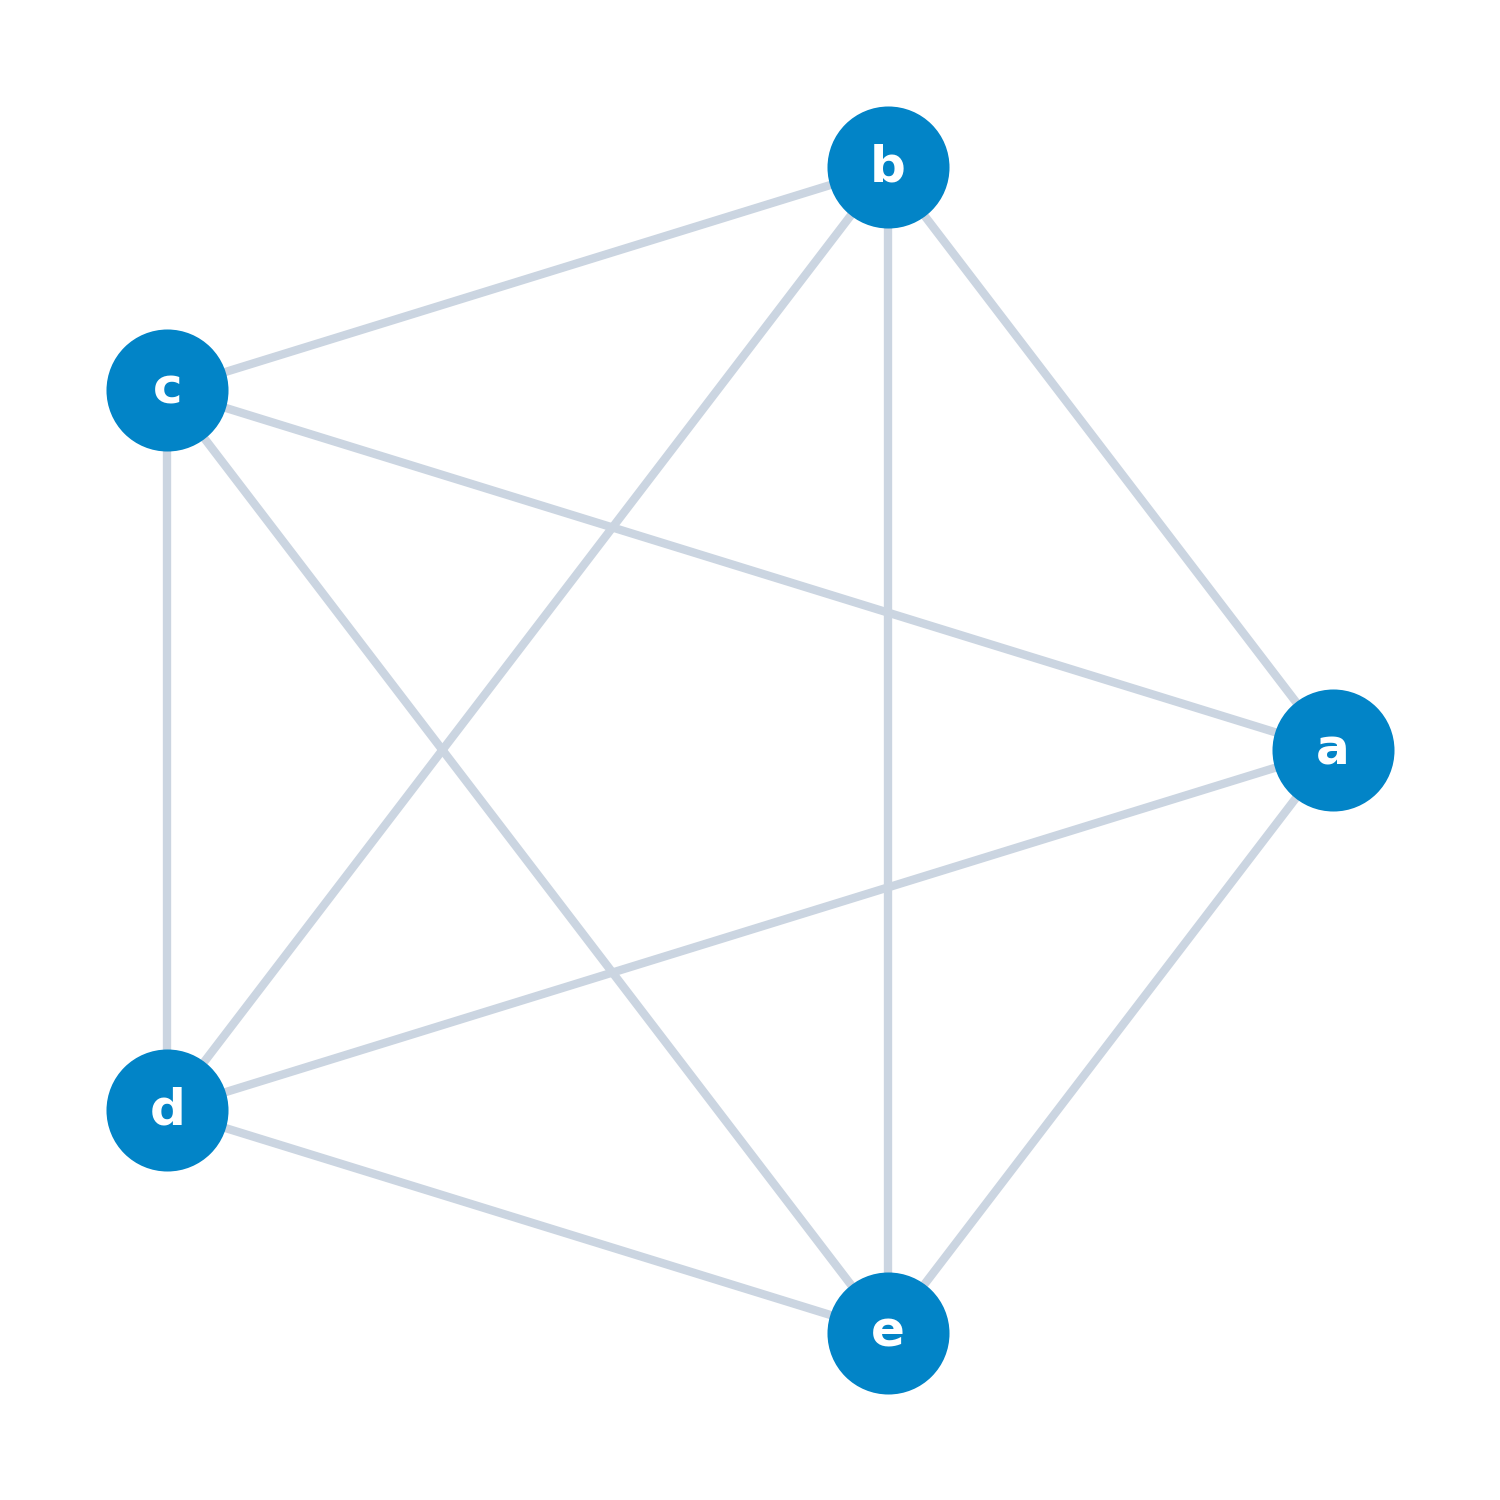
\includegraphics[width=0.9\linewidth,height=\textheight,keepaspectratio]{../images/clan_k5_ejemplo.png}
\end{center}
\end{column}
\end{columns}
\end{column}
\end{columns}
\end{frame}

\begin{frame}{Digrafos completos}
\phantomsection\label{digrafos-completos}
\begin{columns}[T]
\begin{column}{0.55\linewidth}
\begin{tcolorbox}[enhanced jigsaw, toptitle=1mm, opacityback=0, opacitybacktitle=0.6, colback=white, arc=.35mm, bottomrule=.15mm, titlerule=0mm, coltitle=black, breakable, bottomtitle=1mm, left=2mm, title=\textcolor{quarto-callout-note-color}{\faInfo}\hspace{0.5em}{Definición: Digrafo completo}, colbacktitle=quarto-callout-note-color!10!white, rightrule=.15mm, toprule=.15mm, colframe=quarto-callout-note-color-frame, leftrule=.75mm]

Un digrafo \(G = (V, U)\) se dice \textbf{completo} si para todo par de
vértices distintos \(i \neq j\), la ausencia de un arco en una dirección
implica la existencia obligatoria del arco en sentido inverso: \[
(i, j) \notin U \implies (j, i) \in U \quad (\forall i \neq j)
\]

\end{tcolorbox}

\begin{itemize}
\tightlist
\item
  \textbf{Interpretación orientada}: Se garantiza al menos un sentido de
  comunicación directa entre cualquier pareja de vértices.
\end{itemize}
\end{column}

\begin{column}{0.45\linewidth}
\pandocbounded{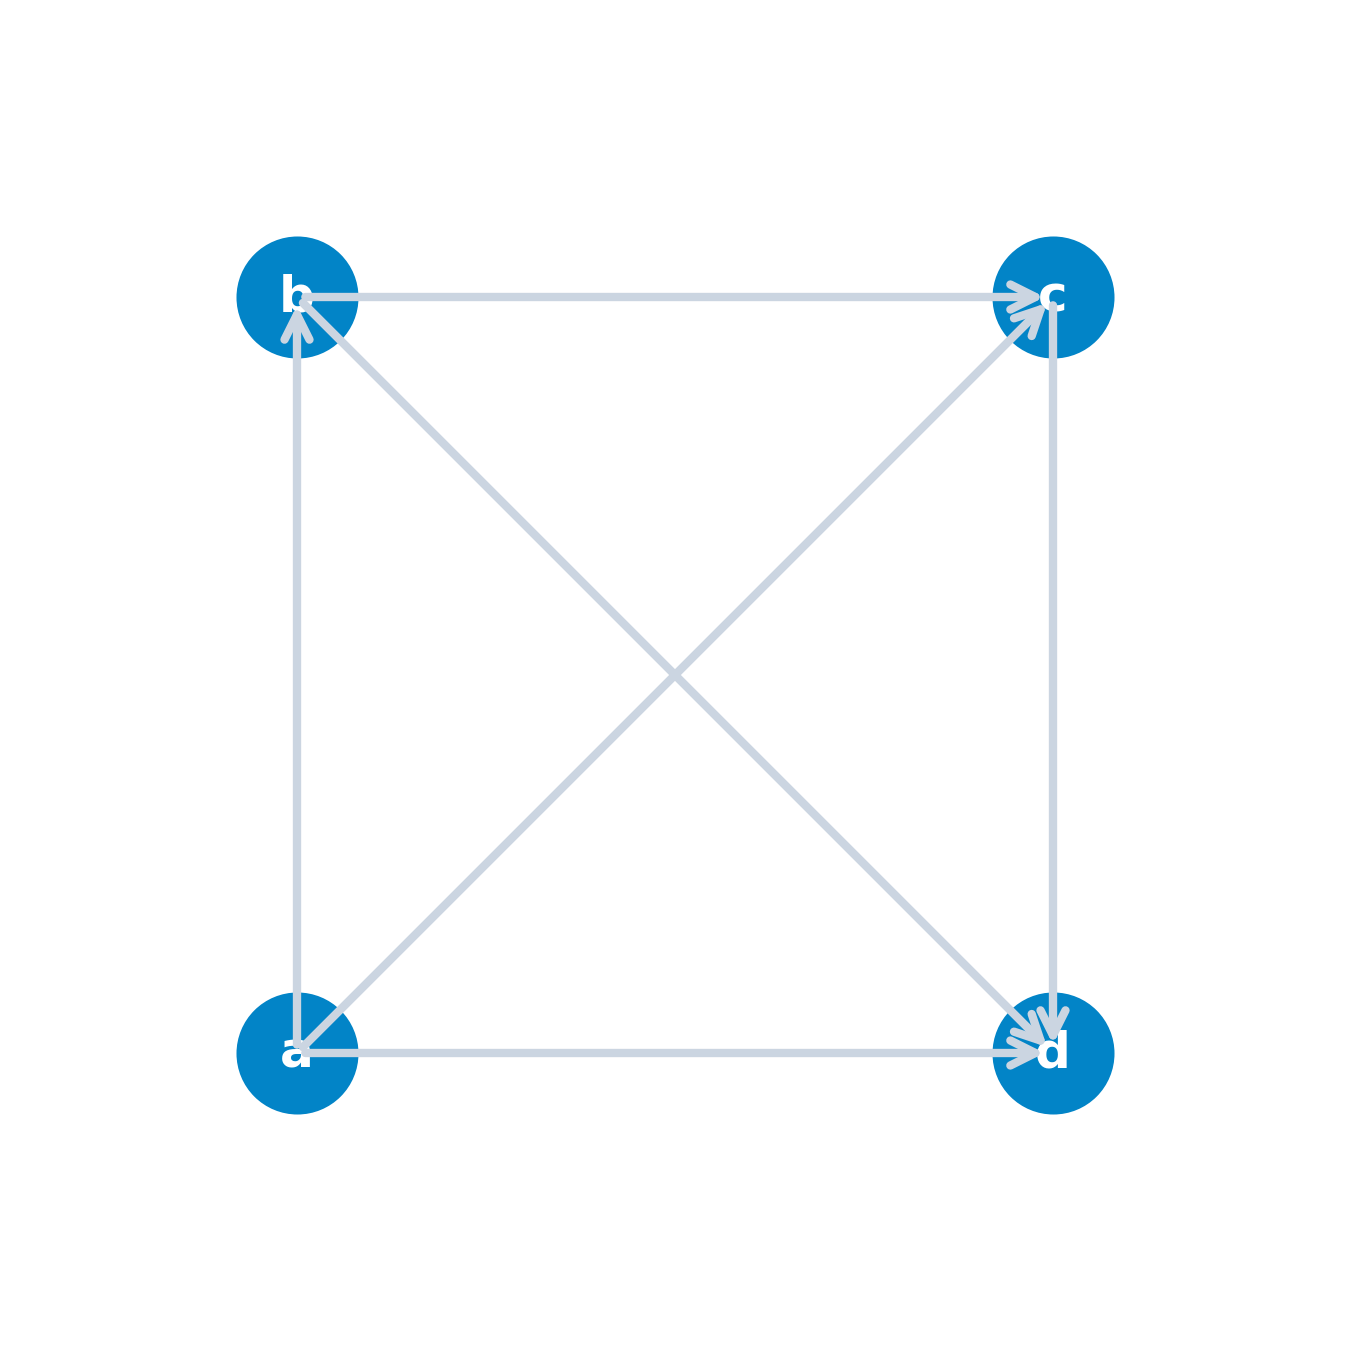
\includegraphics[keepaspectratio]{../images/digrafo_completo_ejemplo.png}}
\end{column}
\end{columns}
\end{frame}

\begin{frame}{Grafo base original de referencia \(G = (V, U)\)}
\phantomsection\label{grafo-base-original-de-referencia-g-v-u}
\begin{columns}[T]
\begin{column}{0.5\linewidth}
\begin{itemize}
\tightlist
\item
  \textbf{Digrafo original de referencia}: Red orientada \(G = (V, U)\)
  compuesta por \(n=5\) nodos (\(V=\{1,2,3,4,5\}\)) y 7 arcos.
\item
  \textbf{Operaciones de subestructura}: A partir de esta red base se
  definen:

  \begin{itemize}
  \tightlist
  \item
    \textbf{Subgrafos inducidos}: Selección de un subconjunto de nodos
    \(A \subset V\).
  \item
    \textbf{Grafos parciales}: Selección de un subconjunto de arcos
    \(W \subset U\).
  \end{itemize}
\end{itemize}
\end{column}

\begin{column}{0.5\linewidth}
\pandocbounded{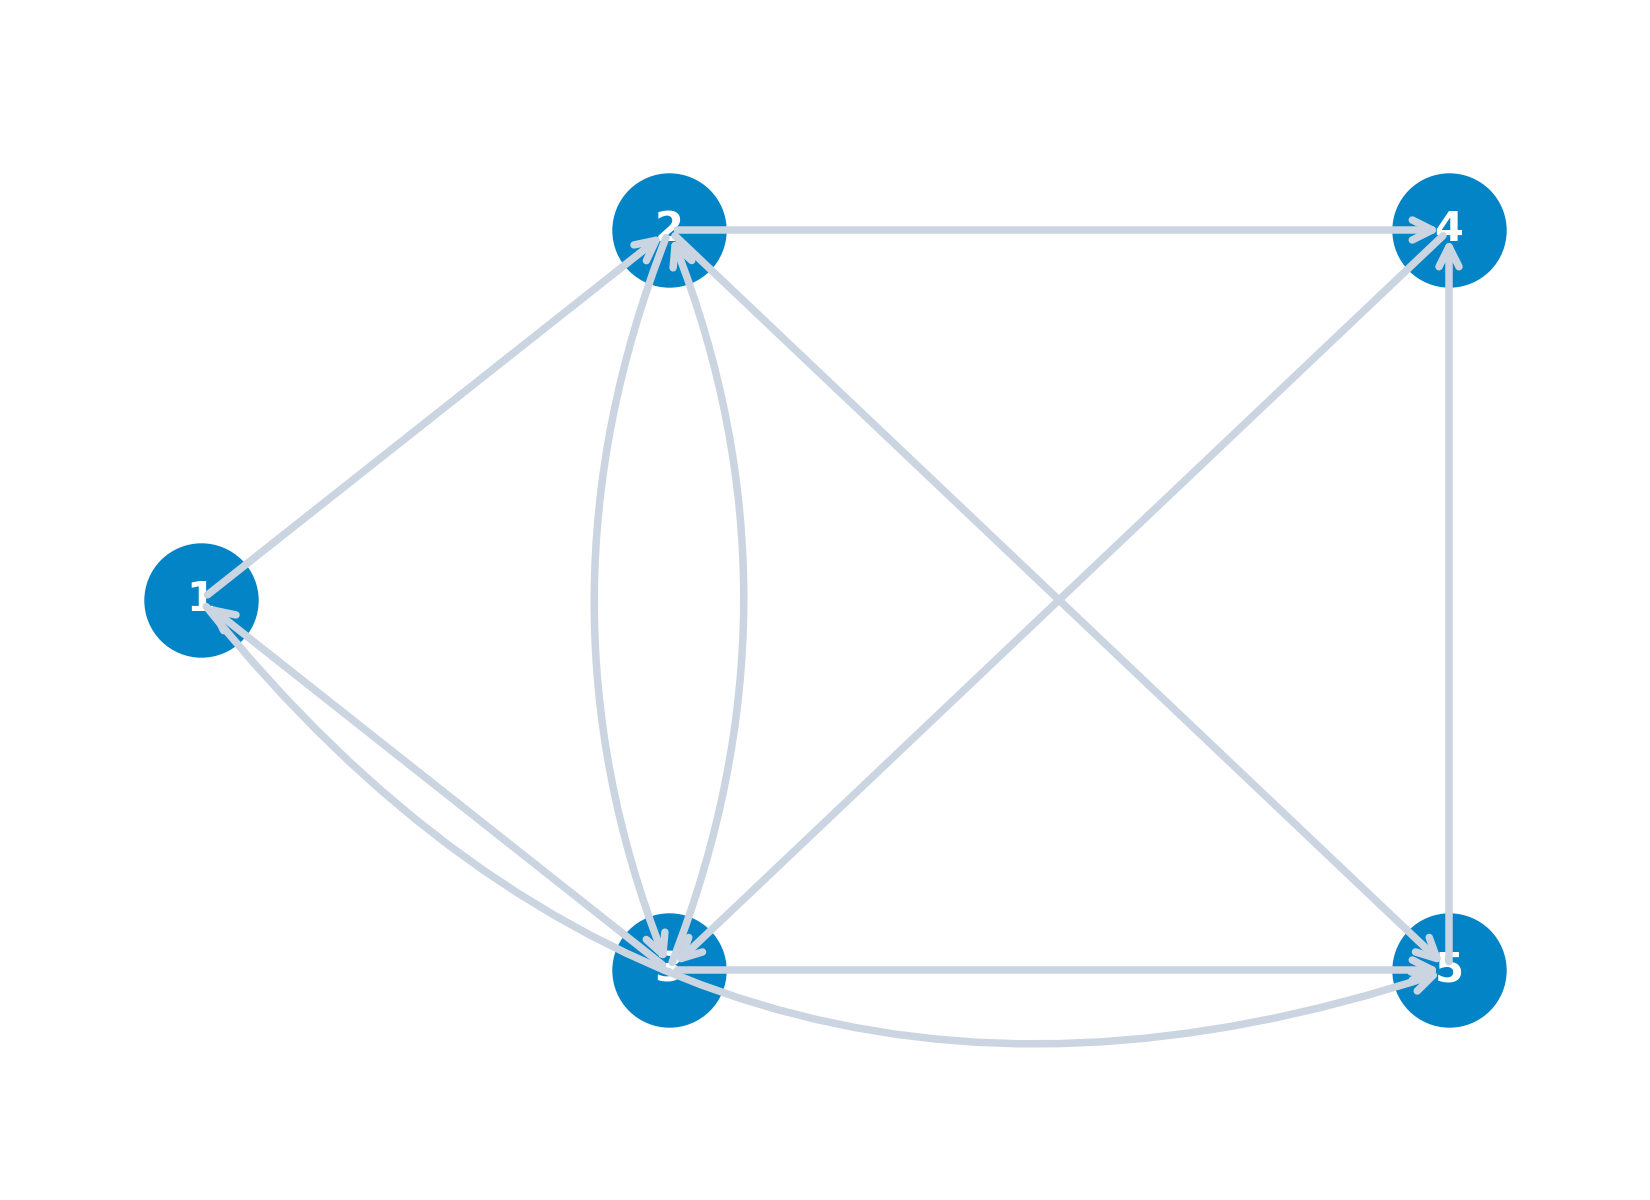
\includegraphics[keepaspectratio]{../images/digrafo_base_original.png}}
\end{column}
\end{columns}
\end{frame}

\begin{frame}{Subgrafos inducidos (por nodos)}
\phantomsection\label{subgrafos-inducidos-por-nodos}
\begin{columns}[T]
\begin{column}{0.55\linewidth}
\begin{tcolorbox}[enhanced jigsaw, toptitle=1mm, opacityback=0, opacitybacktitle=0.6, colback=white, arc=.35mm, bottomrule=.15mm, titlerule=0mm, coltitle=black, breakable, bottomtitle=1mm, left=2mm, title=\textcolor{quarto-callout-note-color}{\faInfo}\hspace{0.5em}{Definición: Subgrafo inducido}, colbacktitle=quarto-callout-note-color!10!white, rightrule=.15mm, toprule=.15mm, colframe=quarto-callout-note-color-frame, leftrule=.75mm]

Dado \(G = (V, U)\) y un subconjunto de vértices \(A \subset V\), el
\textbf{subgrafo inducido} \(G_A = (A, U_A)\) conserva únicamente los
nodos de \(A\) y los arcos con ambos extremos en \(A\): \[
U_A = \{(i, j) \in U : i, j \in A\}
\]

\end{tcolorbox}

\begin{itemize}
\tightlist
\item
  \textbf{Ejemplo para \(A=\{1,2,5\}\)}: Los nodos \(\{3, 4\}\) y sus
  arcos incidentes desaparecen por completo respecto a la red base
  \(G\).
\end{itemize}
\end{column}

\begin{column}{0.45\linewidth}
\pandocbounded{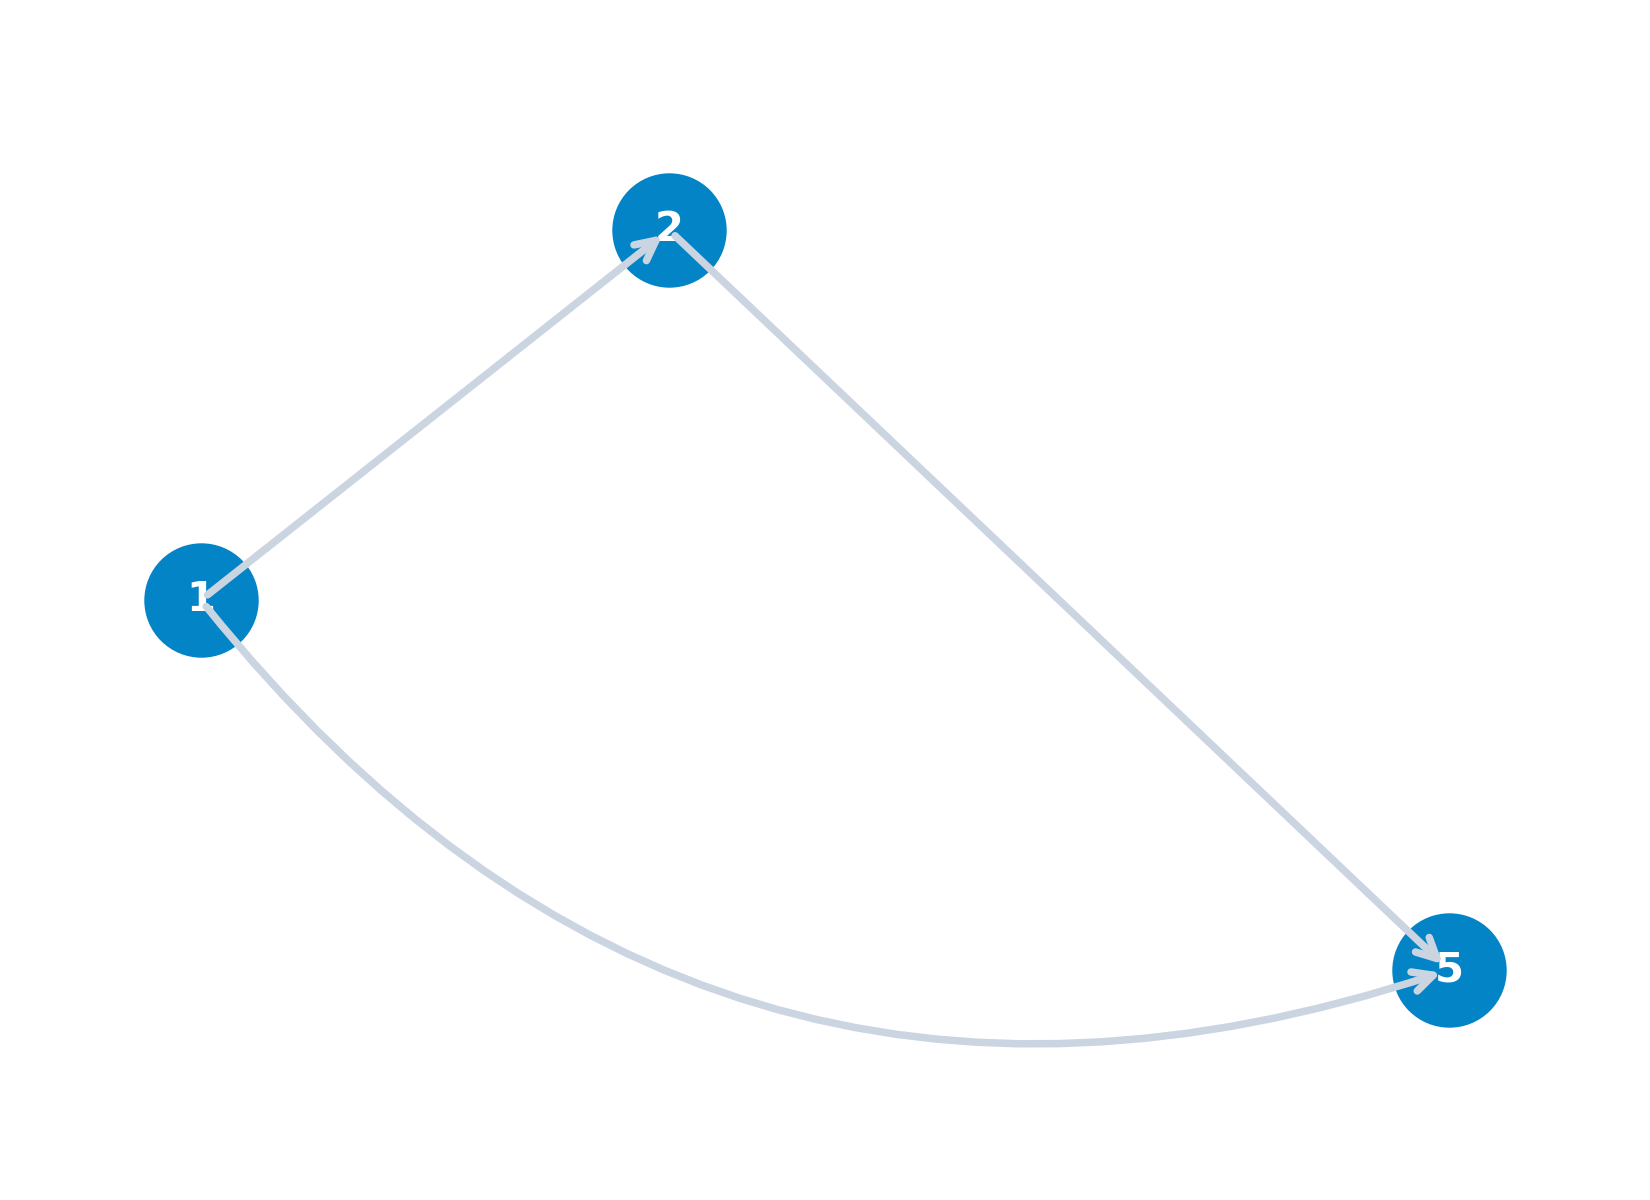
\includegraphics[keepaspectratio]{../images/subgrafo_inducido_a125.png}}
\end{column}
\end{columns}
\end{frame}

\begin{frame}{Grafos parciales (por arcos)}
\phantomsection\label{grafos-parciales-por-arcos}
\begin{columns}[T]
\begin{column}{0.55\linewidth}
\begin{tcolorbox}[enhanced jigsaw, toptitle=1mm, opacityback=0, opacitybacktitle=0.6, colback=white, arc=.35mm, bottomrule=.15mm, titlerule=0mm, coltitle=black, breakable, bottomtitle=1mm, left=2mm, title=\textcolor{quarto-callout-note-color}{\faInfo}\hspace{0.5em}{Definición: Grafo parcial}, colbacktitle=quarto-callout-note-color!10!white, rightrule=.15mm, toprule=.15mm, colframe=quarto-callout-note-color-frame, leftrule=.75mm]

Dado \(G = (V, U)\) y un subconjunto de arcos \(W \subset U\), el
\textbf{grafo parcial} \(G(W) = (V, W)\) conserva los \(n\) vértices de
\(V\), restringiendo los arcos a \(W\).

\end{tcolorbox}

\begin{itemize}
\tightlist
\item
  \textbf{Ejemplo para \(W=\{(1,2),(2,4),(5,4)\}\)}: Los \(n=5\) nodos
  de \(G\) se preservan intactos. El nodo 3 permanece presente como
  \textbf{nodo aislado} (\(d(3)=0\)).
\end{itemize}
\end{column}

\begin{column}{0.45\linewidth}
\pandocbounded{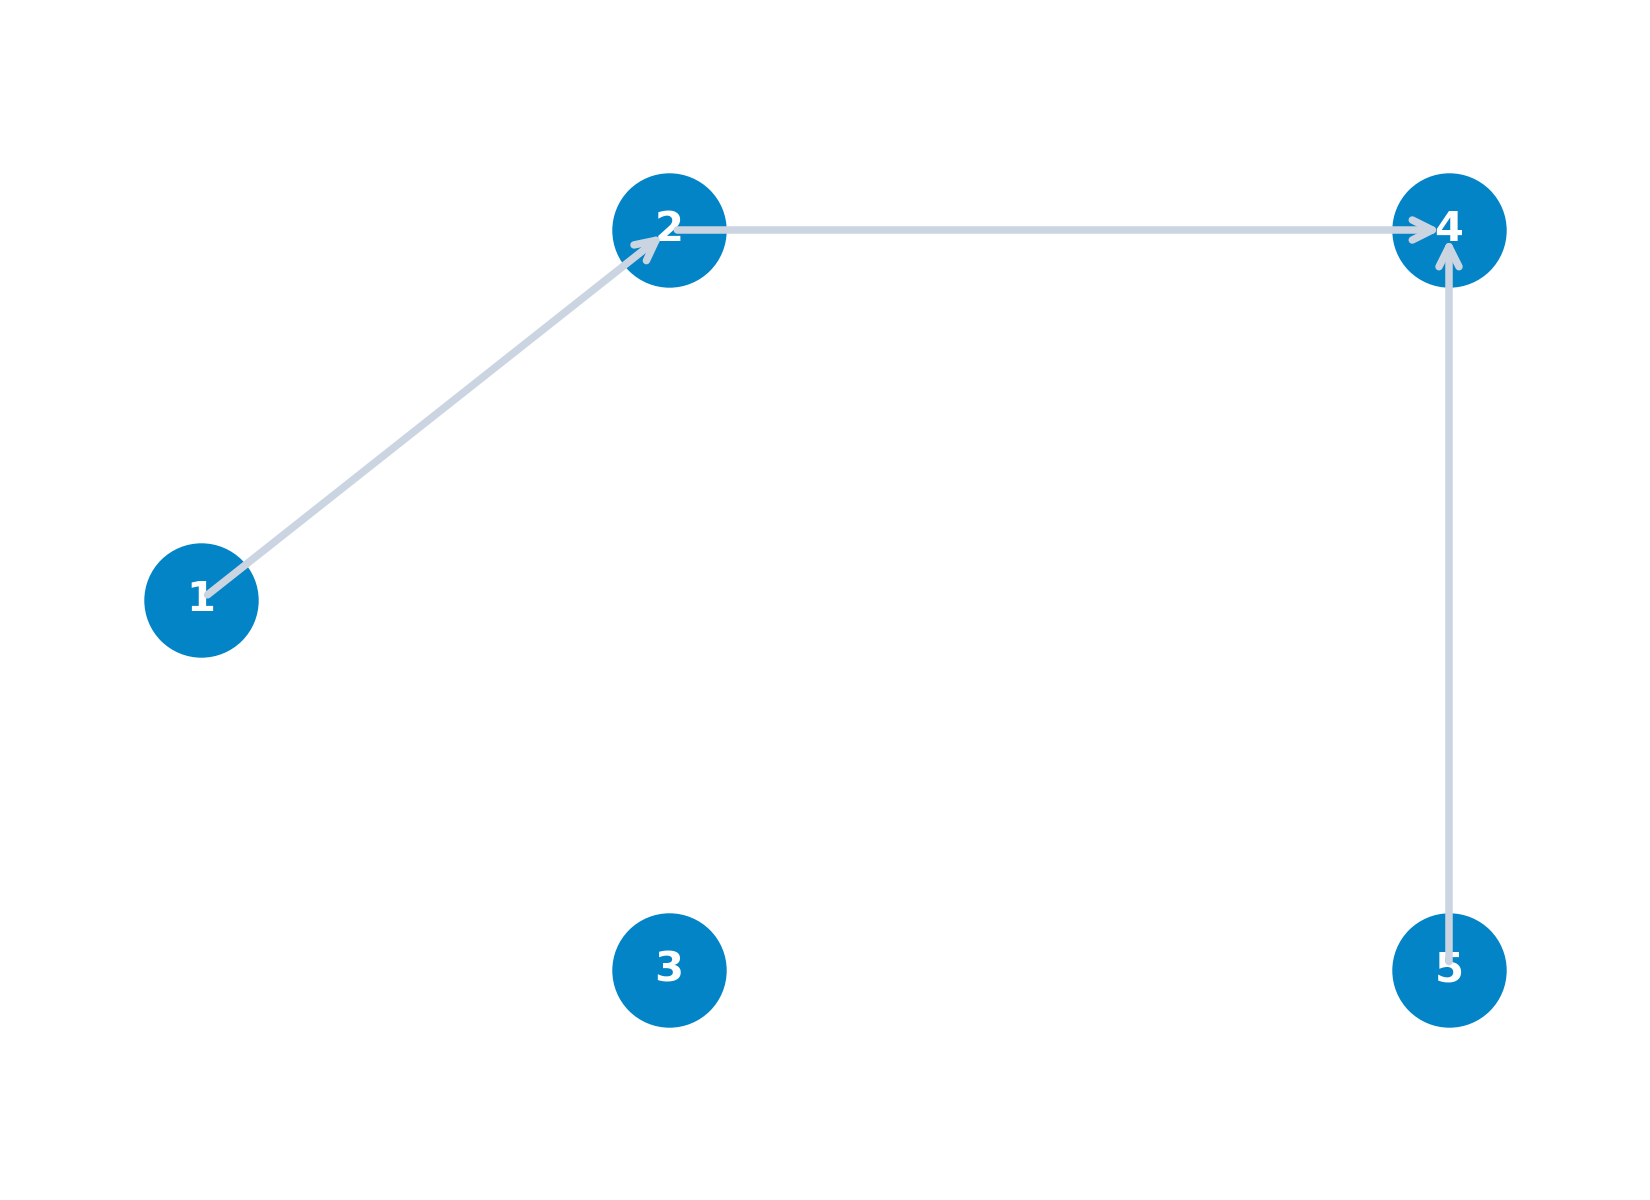
\includegraphics[keepaspectratio]{../images/grafo_parcial_w1.png}}
\end{column}
\end{columns}
\end{frame}

\begin{frame}{Grafo complementario (\(\bar{G}\))}
\phantomsection\label{grafo-complementario-barg}
\begin{columns}[T]
\begin{column}{0.5\linewidth}
\begin{tcolorbox}[enhanced jigsaw, toptitle=1mm, opacityback=0, opacitybacktitle=0.6, colback=white, arc=.35mm, bottomrule=.15mm, titlerule=0mm, coltitle=black, breakable, bottomtitle=1mm, left=2mm, title=\textcolor{quarto-callout-note-color}{\faInfo}\hspace{0.5em}{Definición: Grafo complementario}, colbacktitle=quarto-callout-note-color!10!white, rightrule=.15mm, toprule=.15mm, colframe=quarto-callout-note-color-frame, leftrule=.75mm]

Dado un grafo simple \(G = (V, E)\), su \textbf{grafo complementario}
\(\bar{G} = (V, \bar{E})\) mantiene los mismos vértices y contiene
exactamente las aristas no presentes en \(E\): \[
\{i, j\} \in \bar{E} \iff \{i, j\} \notin E \quad (\forall i \neq j)
\]

\end{tcolorbox}
\end{column}

\begin{column}{0.5\linewidth}
\pandocbounded{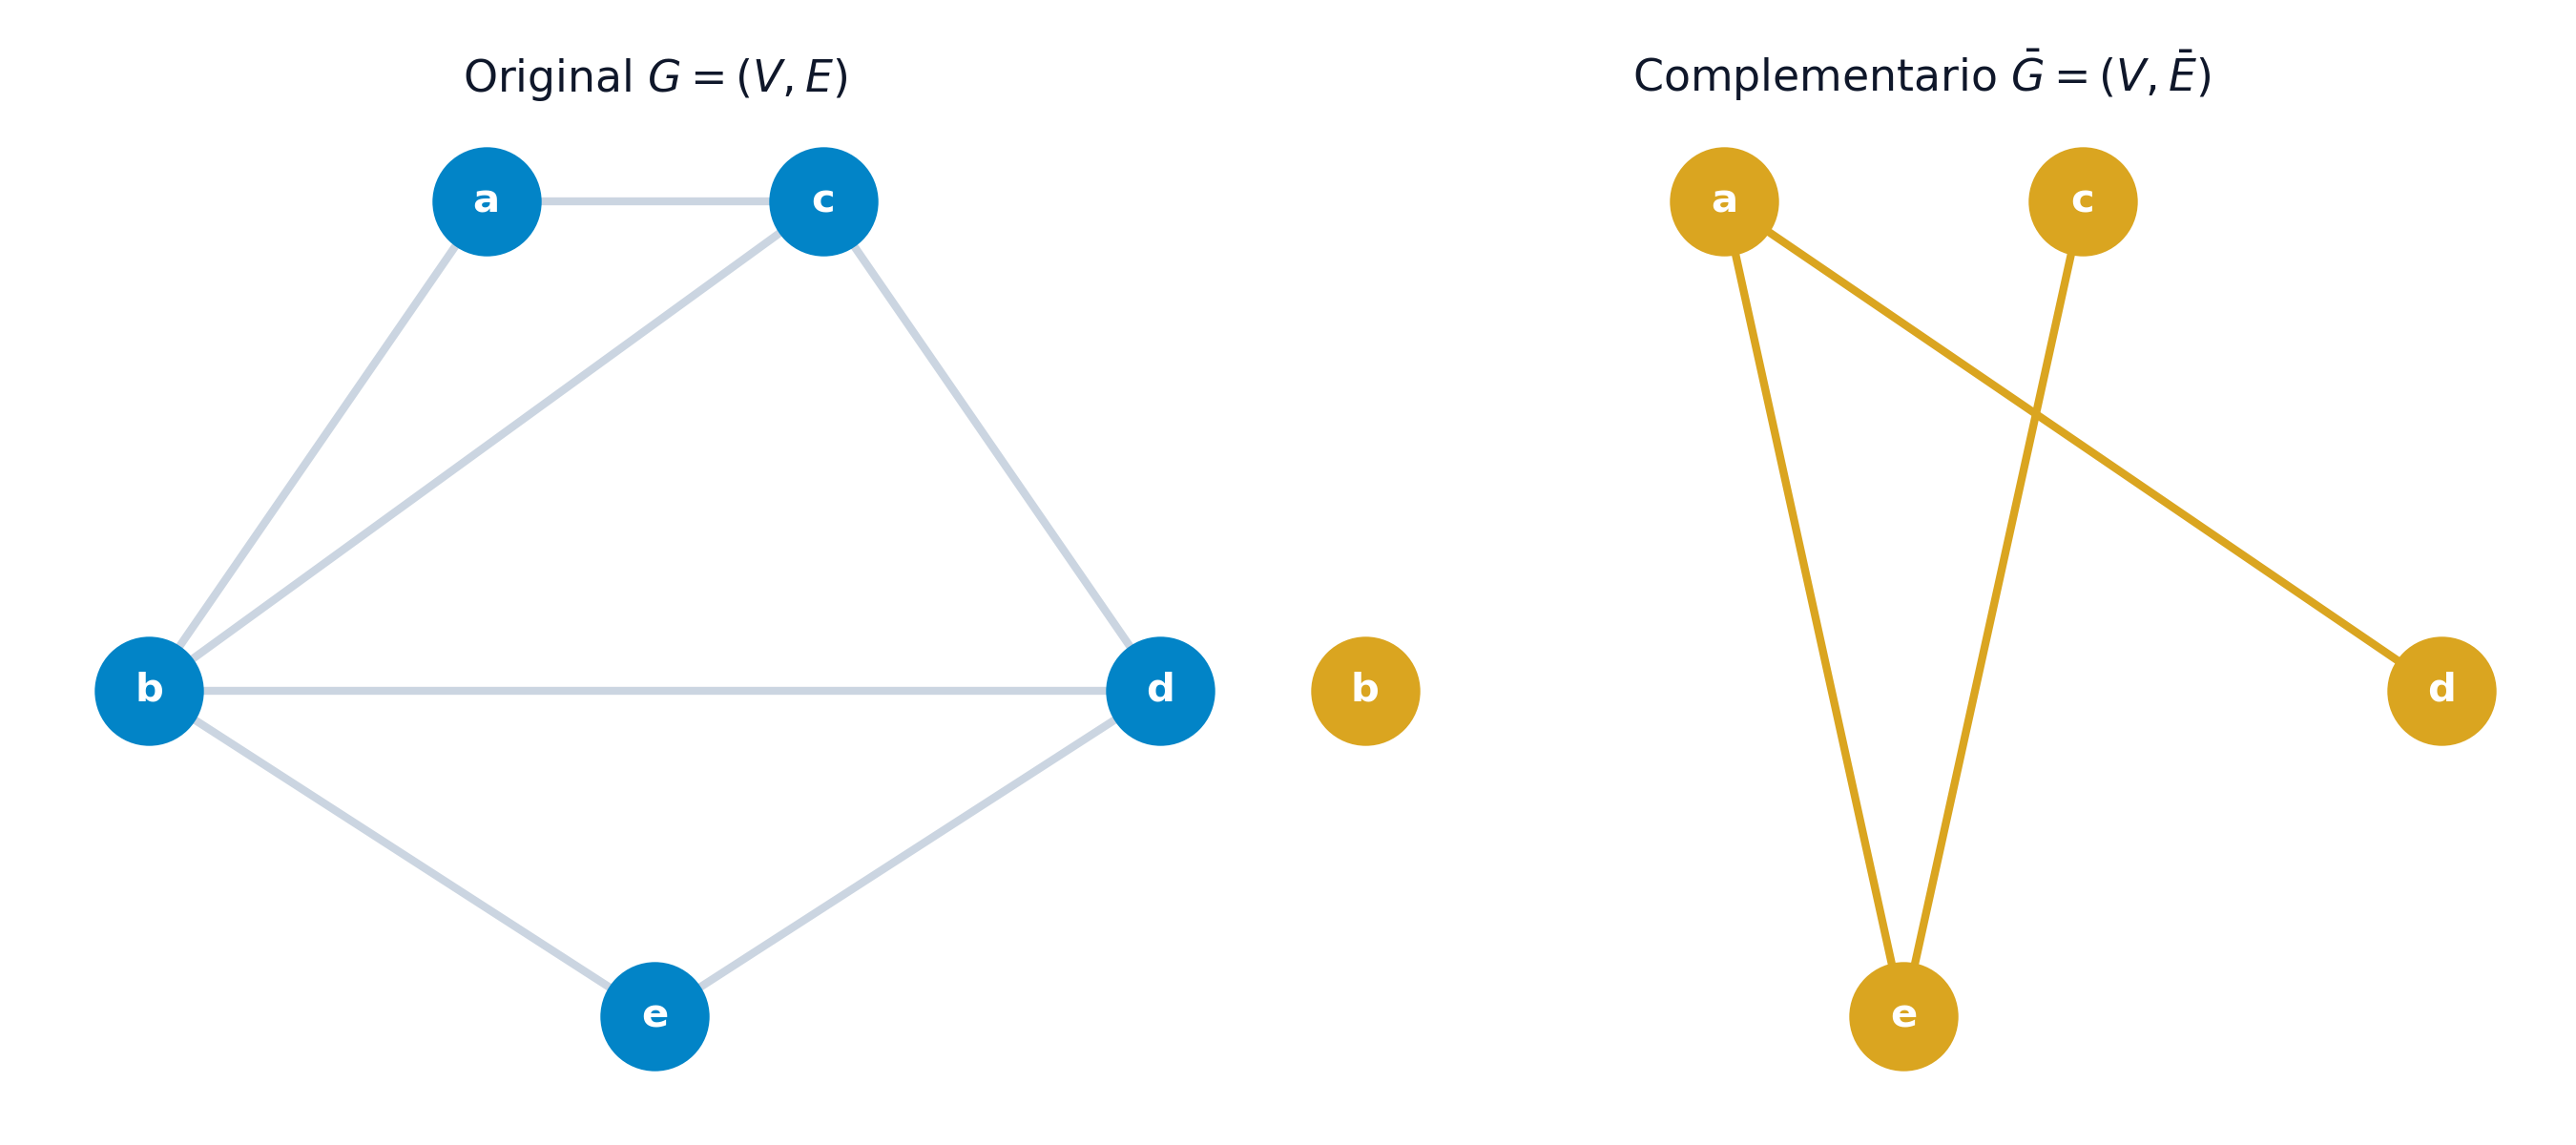
\includegraphics[keepaspectratio]{../images/grafo_complementario.png}}
\end{column}
\end{columns}
\end{frame}

\section{Recorridos y conectividad en
redes}\label{recorridos-y-conectividad-en-redes}

\begin{frame}{Recorridos en redes: Cadenas vs Caminos}
\phantomsection\label{recorridos-en-redes-cadenas-vs-caminos}
\begin{tcolorbox}[enhanced jigsaw, toptitle=1mm, opacityback=0, opacitybacktitle=0.6, colback=white, arc=.35mm, bottomrule=.15mm, titlerule=0mm, coltitle=black, breakable, bottomtitle=1mm, left=2mm, title=\textcolor{quarto-callout-warning-color}{\faExclamationTriangle}\hspace{0.5em}{Diferencia conceptual fundamental}, colbacktitle=quarto-callout-warning-color!10!white, rightrule=.15mm, toprule=.15mm, colframe=quarto-callout-warning-color-frame, leftrule=.75mm]

\begin{itemize}
\tightlist
\item
  \textbf{Cadena \(\mu\)}: Secuencia de arcos adyacentes
  \(\mu = (u_1, u_2, \dots, u_q)\) entre dos nodos que \textbf{no exige
  respetar la orientación de las flechas} (se pueden transitar en
  cualquier sentido). Caracteriza la \textbf{conectividad
  sintáctica/topológica}.
\item
  \textbf{Camino \(P\)}: Secuencia de arcos orientados donde
  \textbf{todos los arcos se transitan strictly a favor de su sentido}
  (\(u_k\) finaliza donde \(u_{k+1}\) comienza). Caracteriza la
  \textbf{posibilidad real de transporte o flujo}.
\item
  \textbf{En redes no dirigidas}, las nociones de cadena y camino
  resultan formalmente equivalentes.
\end{itemize}

\end{tcolorbox}
\end{frame}

\begin{frame}{Propiedades de recorridos: Elementalidad y Simplicidad}
\phantomsection\label{propiedades-de-recorridos-elementalidad-y-simplicidad}
\begin{tcolorbox}[enhanced jigsaw, toptitle=1mm, opacityback=0, opacitybacktitle=0.6, colback=white, arc=.35mm, bottomrule=.15mm, titlerule=0mm, coltitle=black, breakable, bottomtitle=1mm, left=2mm, title=\textcolor{quarto-callout-note-color}{\faInfo}\hspace{0.5em}{Definición: Elementalidad y Simplicidad}, colbacktitle=quarto-callout-note-color!10!white, rightrule=.15mm, toprule=.15mm, colframe=quarto-callout-note-color-frame, leftrule=.75mm]

Dado un digrafo \(G = (V, U)\) o grafo \(G = (V, E)\):

\begin{itemize}
\tightlist
\item
  \textbf{Elemental}: Una cadena o camino es \textbf{elemental} si
  \textbf{no repite ningún vértice} en su secuencia.
\item
  \textbf{Simple}: Una cadena o camino es \textbf{simple} si \textbf{no
  repite ningún arco o arista} en su secuencia.
\end{itemize}

\end{tcolorbox}

\begin{itemize}
\tightlist
\item
  \textbf{Red de aeropuertos de referencia}:
  \(V = \{m, l, p, f, s, t\}\) (Madrid, Londres, París, Frankfurt,
  Singapur, Tokio).
\end{itemize}
\end{frame}

\begin{frame}{Ejemplo 1: Cadena elemental y simple (\(\mu^1\))}
\phantomsection\label{ejemplo-1-cadena-elemental-y-simple-mu1}
\begin{columns}[T]
\begin{column}{0.5\linewidth}
\begin{itemize}
\tightlist
\item
  \textbf{Cadena \(\mu^1[m, p]\) de longitud \(q=3\)}:
  \[\mu^1 = \{(m, l), (l, f), (p, f)\}\]
\item
  Recorre \(\{m, l, f, p\}\) sin repetir ninguno \(\implies\)
  \textbf{Elemental}.
\item
  Transita por 3 arcos distintos \(\implies\) \textbf{Simple}.
\item
  El arco \((p, f)\) en sentido inverso \(\implies\) Es una
  \textbf{cadena} (no un camino).
\end{itemize}
\end{column}

\begin{column}{0.5\linewidth}
\pandocbounded{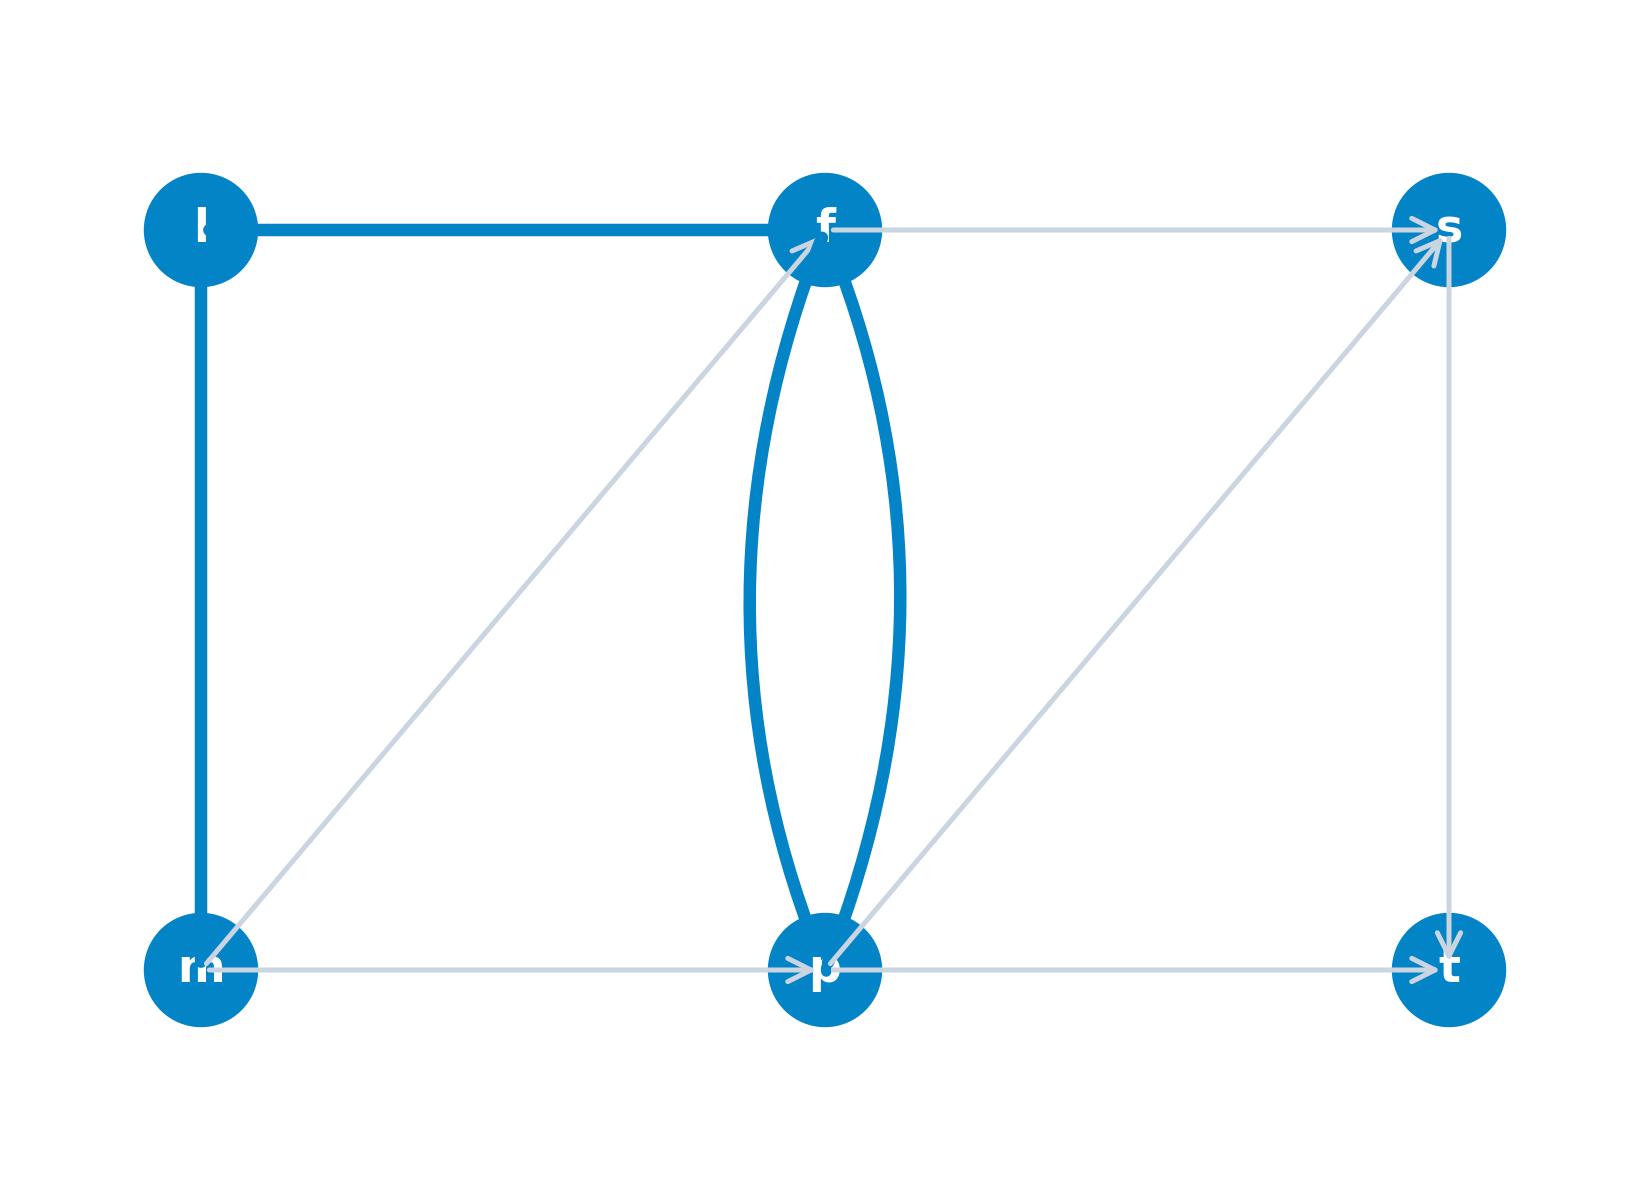
\includegraphics[keepaspectratio]{../images/cadena_ejemplo_mu1.png}}
\end{column}
\end{columns}
\end{frame}

\begin{frame}{Ejemplo 2: Camino elemental y simple (\(\mu^2\))}
\phantomsection\label{ejemplo-2-camino-elemental-y-simple-mu2}
\begin{columns}[T]
\begin{column}{0.5\linewidth}
\begin{itemize}
\tightlist
\item
  \textbf{Camino \(\mu^2[p, t]\) de longitud \(q=3\)}:
  \[\mu^2 = \{(p, f), (f, s), (s, t)\}\]
\item
  Todos los arcos en sentido directo (\(p \to f \to s \to t\))
  \(\implies\) Es un \textbf{camino}.
\item
  No repite ningún vértice \(\implies\) \textbf{Elemental}.
\item
  No repite ningún arco \(\implies\) \textbf{Simple}.
\end{itemize}
\end{column}

\begin{column}{0.5\linewidth}
\pandocbounded{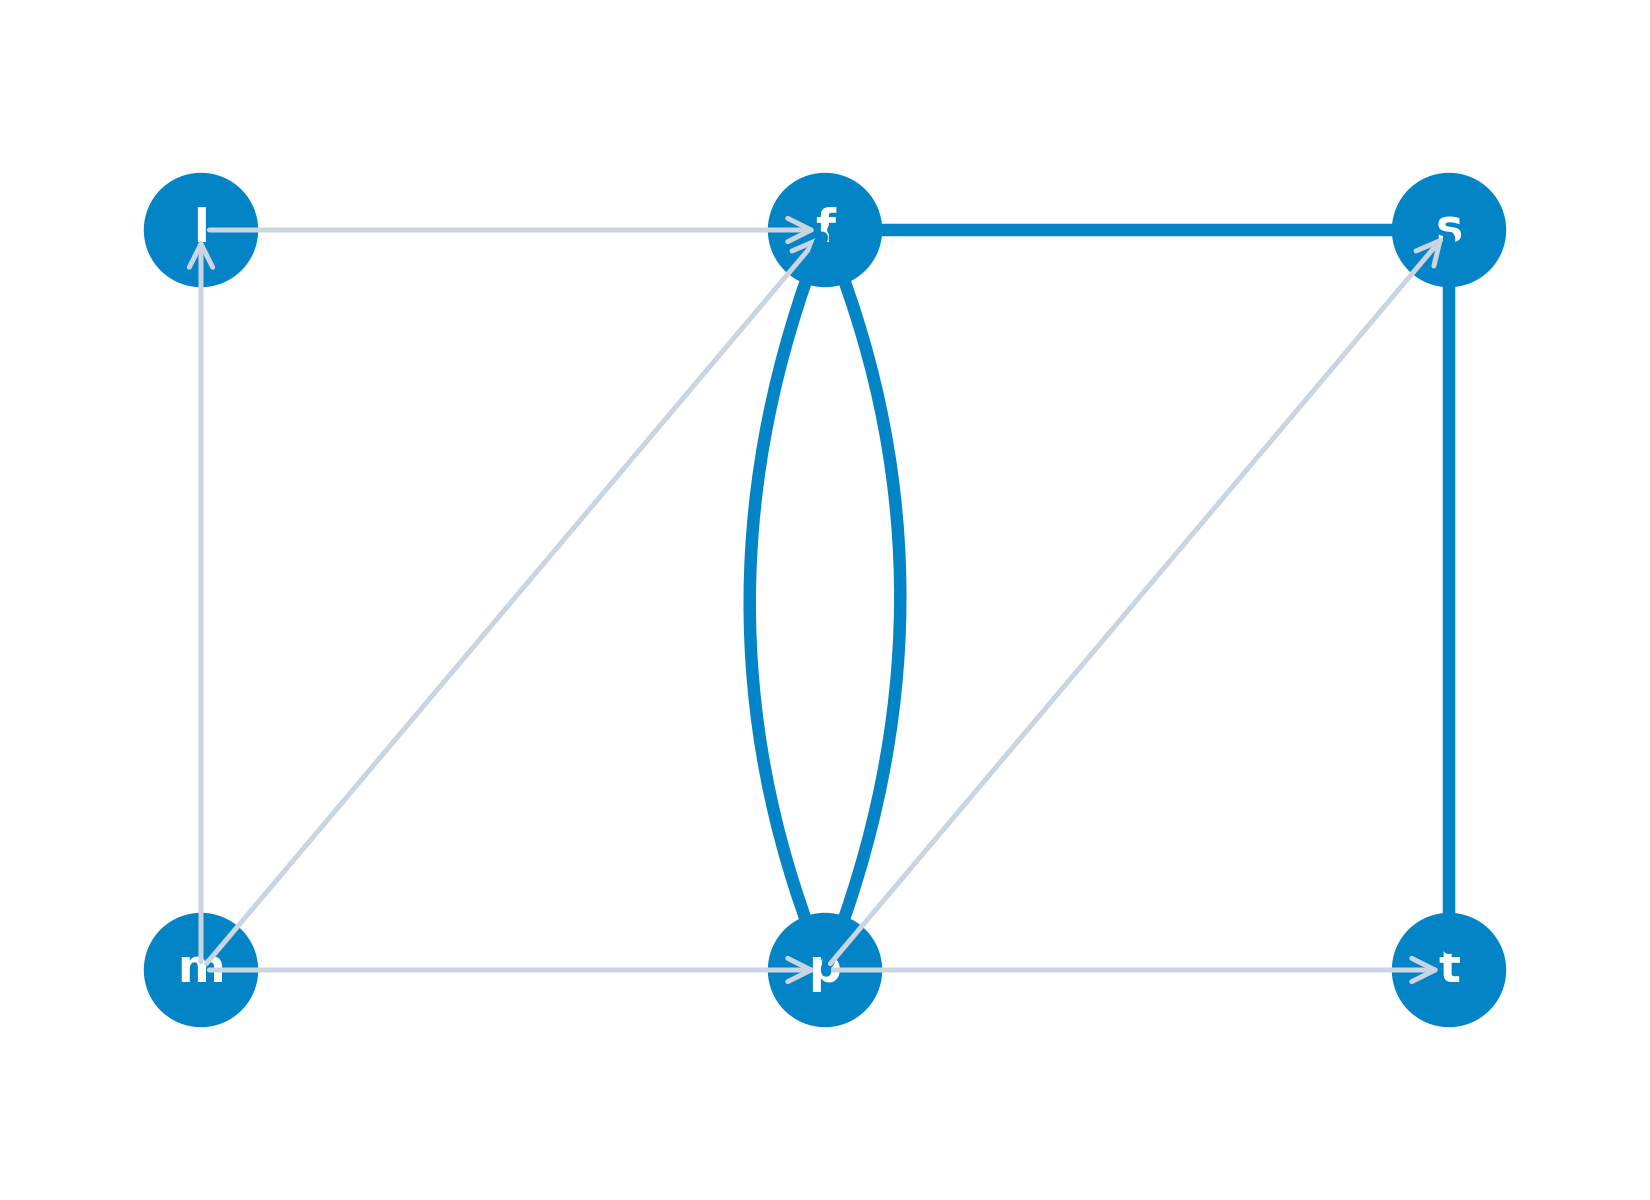
\includegraphics[keepaspectratio]{../images/cadena_ejemplo_mu2.png}}
\end{column}
\end{columns}
\end{frame}

\begin{frame}{Ejemplo 3: Cadena simple no elemental (\(\mu^3\))}
\phantomsection\label{ejemplo-3-cadena-simple-no-elemental-mu3}
\begin{columns}[T]
\begin{column}{0.5\linewidth}
\begin{itemize}
\tightlist
\item
  \textbf{Cadena \(\mu^3[m, p]\) de longitud \(q=5\)}: \[
  \begin{aligned}
  \mu^3 = \{ &(m, p), (p, f), (f, s), \\
             &(p, s), (p, t) \}
  \end{aligned}
  \]
\item
  Visita el nodo París (\(p\)) dos veces
  (\(m \to p \to f \to s \to p \to t\)) \(\implies\) \textbf{No
  elemental}.
\item
  No repite ninguno de sus 5 arcos \(\implies\) \textbf{Simple}.
\end{itemize}
\end{column}

\begin{column}{0.5\linewidth}
\pandocbounded{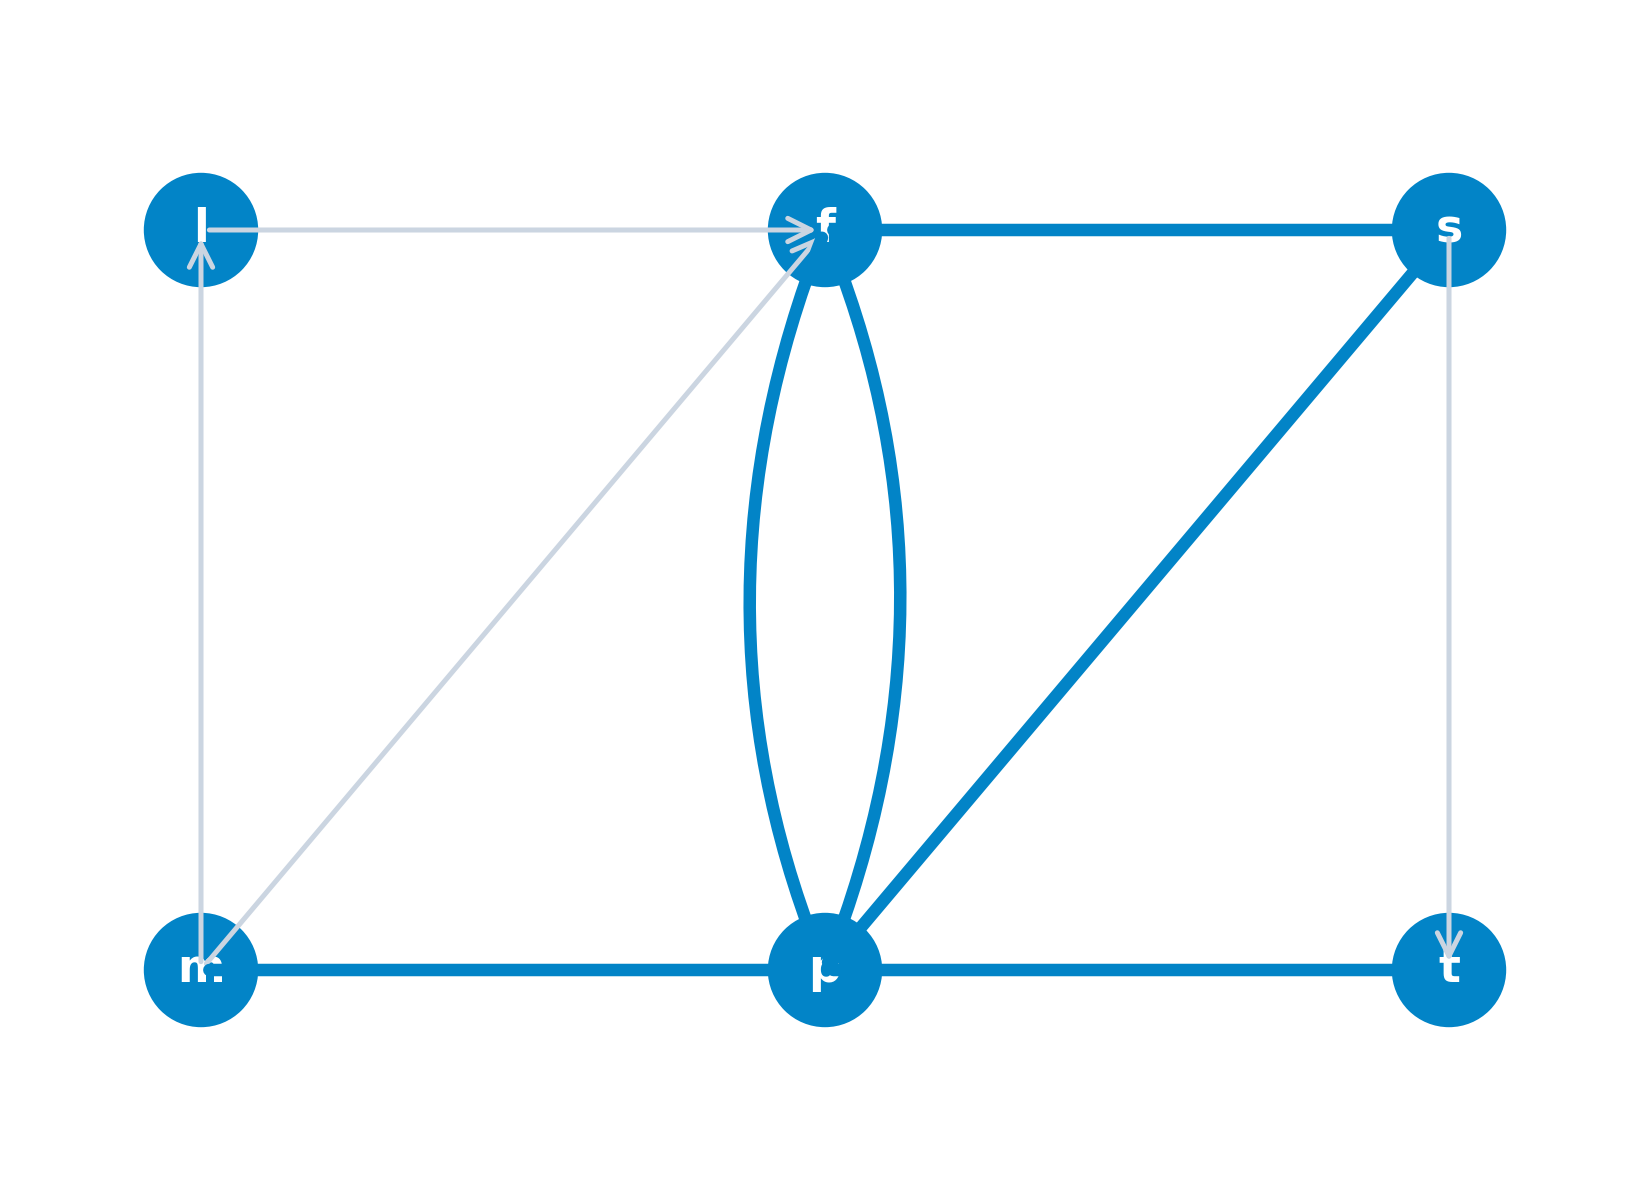
\includegraphics[keepaspectratio]{../images/cadena_ejemplo_mu3.png}}
\end{column}
\end{columns}
\end{frame}

\begin{frame}{Ejemplo 4: Cadena ni elemental ni simple (\(\mu^4\))}
\phantomsection\label{ejemplo-4-cadena-ni-elemental-ni-simple-mu4}
\begin{columns}[T]
\begin{column}{0.5\linewidth}
\begin{itemize}
\tightlist
\item
  \textbf{Cadena \(\mu^4\) de longitud \(q=6\)}: \[
  \begin{aligned}
  \mu^4 = \{ &(l, f), (f, s), (p, s), \\
             &(p, f), (f, s), (s, t) \}
  \end{aligned}
  \]
\item
  Visita nodos repetidos (\(f, s, p\)) \(\implies\) \textbf{No
  elemental}.
\item
  Duplica el tránsito por el arco \((f, s)\) dos veces \(\implies\)
  \textbf{No simple}.
\end{itemize}
\end{column}

\begin{column}{0.5\linewidth}
\pandocbounded{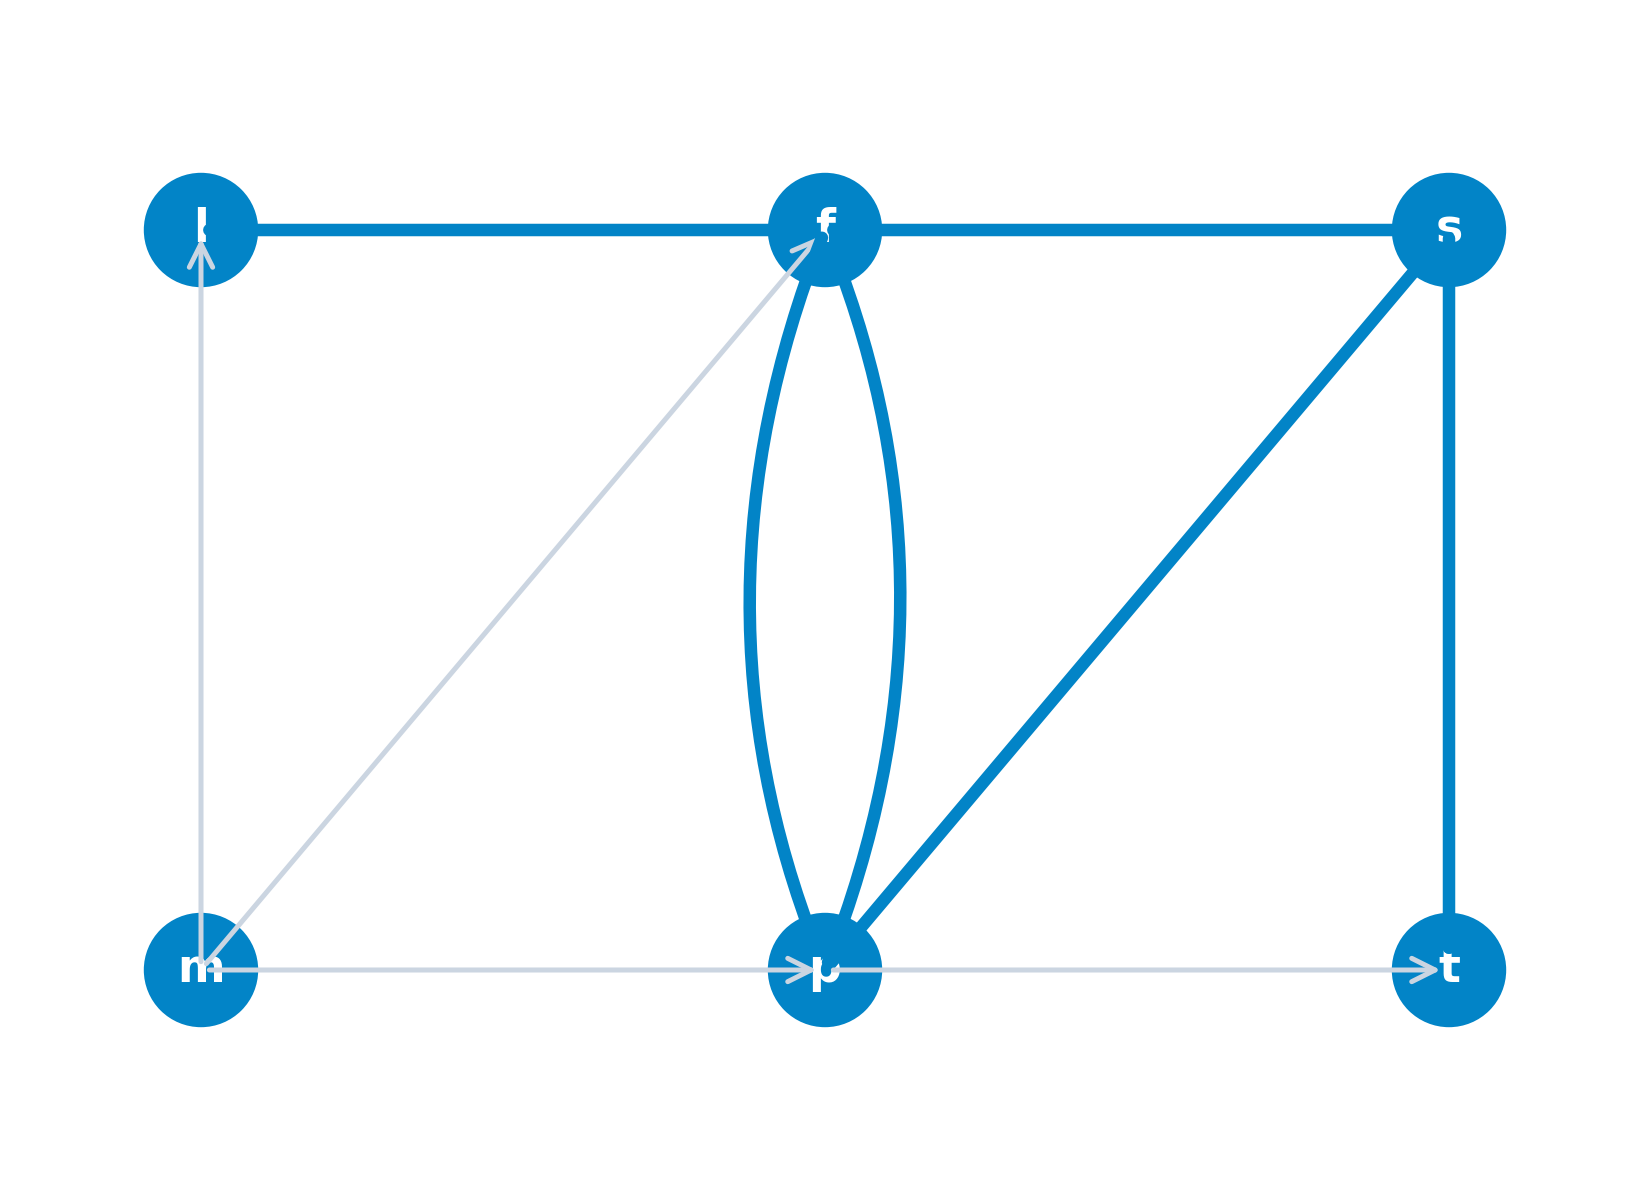
\includegraphics[keepaspectratio]{../images/cadena_ejemplo_mu4.png}}
\end{column}
\end{columns}
\end{frame}

\begin{frame}{Ejemplo: Clasificación de cadenas (Análisis analítico)}
\phantomsection\label{ejemplo-clasificaciuxf3n-de-cadenas-anuxe1lisis-analuxedtico}
Evaluación sobre un grafo no dirigido de 5 vértices
\(V = \{1, 2, 3, 4, 5\}\):

\begin{enumerate}
\tightlist
\item
  \textbf{Cadena \(\mu_1 = \{\{1,2\}, \{2,3\}, \{3,4\}, \{4,5\}\}\)}:

  \begin{itemize}
  \tightlist
  \item
    Visita 5 vértices distintos sin repetir ninguno \(\implies\)
    \textbf{Elemental y simple}.
  \end{itemize}
\item
  \textbf{Cadena
  \(\mu_2 = \{\{1,2\}, \{2,3\}, \{3,4\}, \{4,2\}, \{2,5\}\}\)}:

  \begin{itemize}
  \tightlist
  \item
    Recorre 5 aristas distintas sin repetir ninguna, pero visita el nodo
    2 dos veces \(\implies\) \textbf{Simple pero no elemental}.
  \end{itemize}
\item
  \textbf{Cadena
  \(\mu_3 = \{\{1,2\}, \{2,4\}, \{4,3\}, \{3,2\}, \{2,1\}\}\)}:

  \begin{itemize}
  \tightlist
  \item
    Repite el nodo 2 y duplica la arista \(\{1,2\}\) \(\implies\)
    \textbf{Ni elemental ni simple}.
  \end{itemize}
\end{enumerate}
\end{frame}

\begin{frame}{Ejemplo: Clasificación de cadenas (Animación)}
\phantomsection\label{ejemplo-clasificaciuxf3n-de-cadenas-animaciuxf3n}
\end{frame}

\begin{frame}{Ejemplo: Clasificación de caminos dirigidos (Análisis
analítico)}
\phantomsection\label{ejemplo-clasificaciuxf3n-de-caminos-dirigidos-anuxe1lisis-analuxedtico}
Evaluación sobre una red dirigida de 7 vértices
\(V = \{a, b, c, d, e, f, g\}\):

\begin{enumerate}
\tightlist
\item
  \textbf{Camino \(P_1 = ((a,b), (b,c), (c,e), (e,f))\)}:

  \begin{itemize}
  \tightlist
  \item
    Transita en sentido directo por 5 vértices distintos y 4 arcos
    distintos \(\implies\) \textbf{Elemental y simple}.
  \end{itemize}
\item
  \textbf{Camino \(P_2 = ((c,g), (g,f), (f,b), (b,c), (c,e))\)}:

  \begin{itemize}
  \tightlist
  \item
    No repite arcos, pero el nodo \(c\) se visita dos veces
    (\(c \to g \to f \to b \to c \to e\)) \(\implies\) \textbf{Simple
    pero no elemental}.
  \end{itemize}
\item
  \textbf{Camino \(P_3 = ((c,e), (e,f), (f,b), (b,c), (c,e), (e,g))\)}:

  \begin{itemize}
  \tightlist
  \item
    Repite vértices (\(c, e\)) y duplica el arco \((c,e)\) \(\implies\)
    \textbf{Ni elemental ni simple}.
  \end{itemize}
\end{enumerate}
\end{frame}

\begin{frame}{Ejemplo: Clasificación de caminos dirigidos (Animación)}
\phantomsection\label{ejemplo-clasificaciuxf3n-de-caminos-dirigidos-animaciuxf3n}
\end{frame}

\begin{frame}{Métricas de alcance y Diámetro \(D(G)\)}
\phantomsection\label{muxe9tricas-de-alcance-y-diuxe1metro-dg}
\begin{columns}[T]
\begin{column}{0.5\linewidth}
\begin{tcolorbox}[enhanced jigsaw, toptitle=1mm, opacityback=0, opacitybacktitle=0.6, colback=white, arc=.35mm, bottomrule=.15mm, titlerule=0mm, coltitle=black, breakable, bottomtitle=1mm, left=2mm, title=\textcolor{quarto-callout-note-color}{\faInfo}\hspace{0.5em}{Definición: Distancia y Diámetro}, colbacktitle=quarto-callout-note-color!10!white, rightrule=.15mm, toprule=.15mm, colframe=quarto-callout-note-color-frame, leftrule=.75mm]

\begin{itemize}
\tightlist
\item
  \textbf{Longitud}: Número de arcos \(q\) en la cadena.
\item
  \textbf{Distancia geodésica \(d(i, j)\)}: Longitud de la cadena más
  corta entre \(i\) y \(j\).
\item
  \textbf{Diámetro \(D(G)\)}: Mayor distancia geodésica entre cualquier
  par de nodos: \[
  D(G) = \max_{i, j \in V} d(i, j)
  \]
\end{itemize}

\end{tcolorbox}
\end{column}

\begin{column}{0.5\linewidth}
\pandocbounded{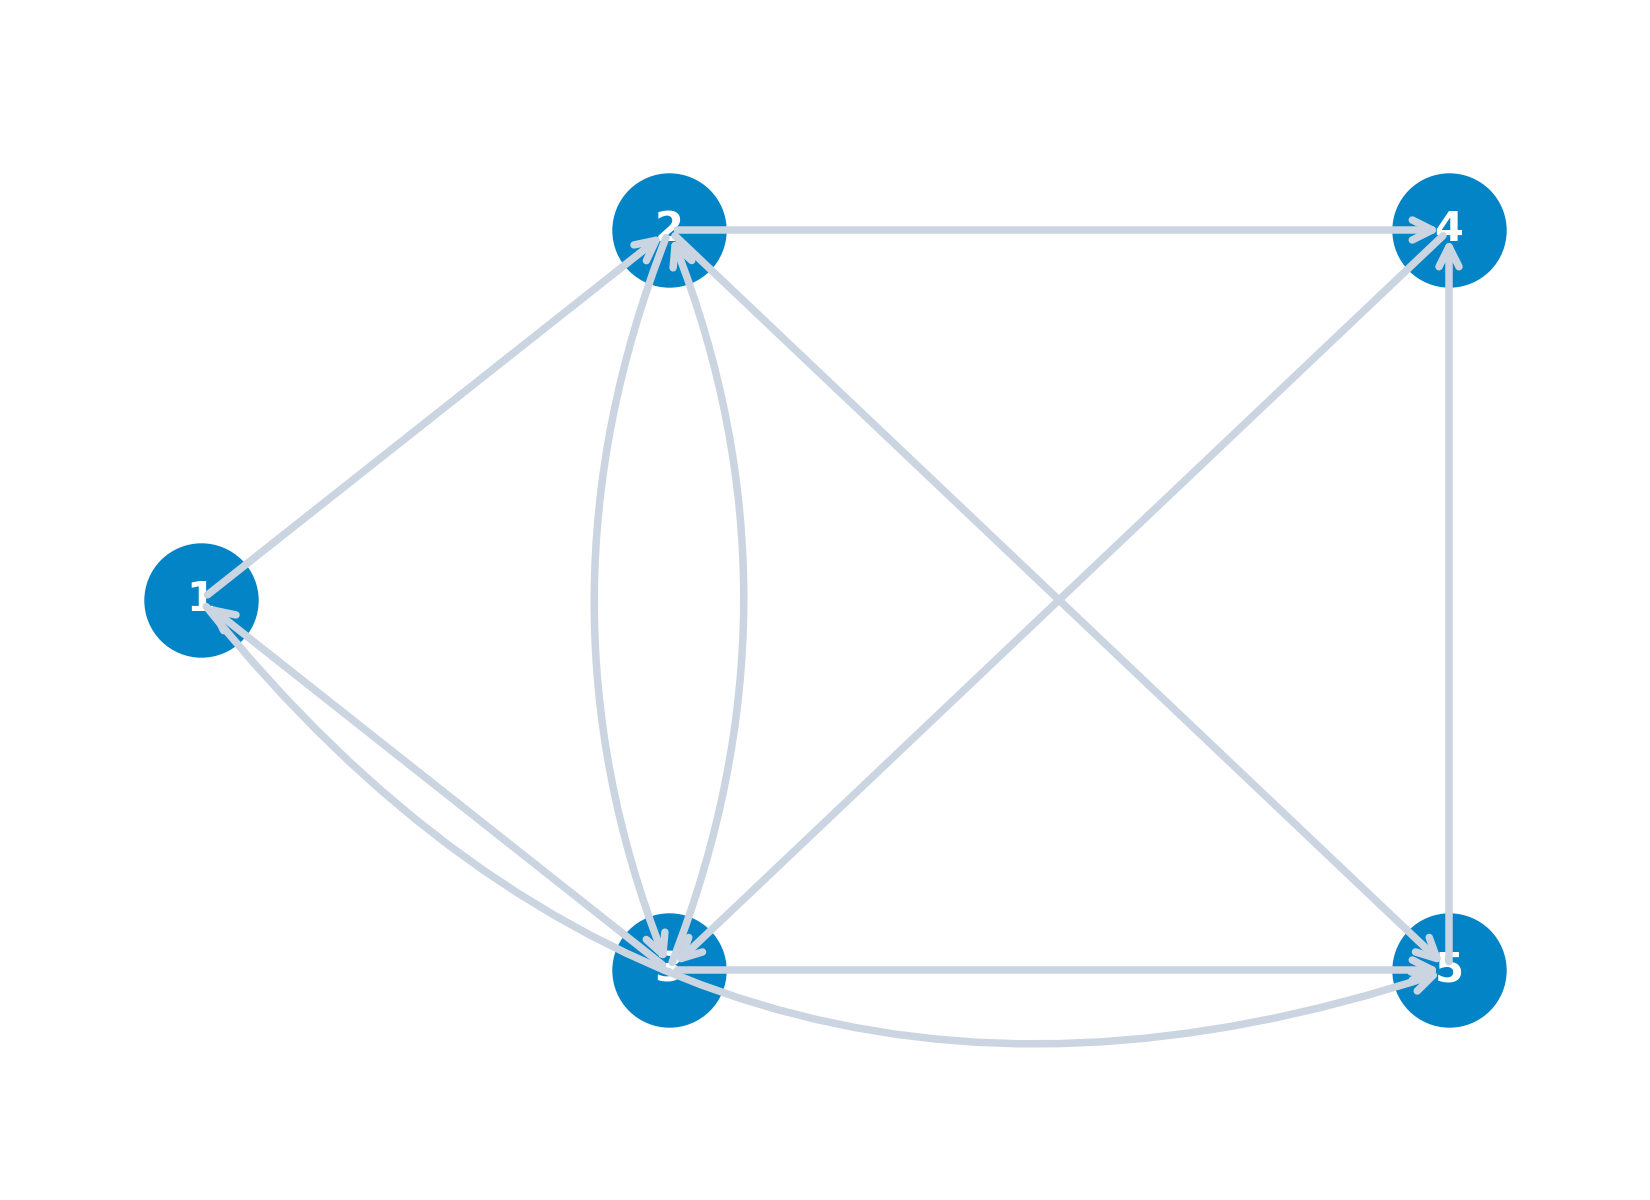
\includegraphics[keepaspectratio]{../images/diametro_grafo_ejemplo.png}}

\begin{itemize}
\tightlist
\item
  En esta red de 5 nodos, la máxima distancia geodésica requerida para
  comunicar cualquier par es de 2 arcos \(\implies D(G) = 2\).
\end{itemize}
\end{column}
\end{columns}
\end{frame}

\begin{frame}{Conectividad y conexidad fuerte}
\phantomsection\label{conectividad-y-conexidad-fuerte}
\begin{tcolorbox}[enhanced jigsaw, toptitle=1mm, opacityback=0, opacitybacktitle=0.6, colback=white, arc=.35mm, bottomrule=.15mm, titlerule=0mm, coltitle=black, breakable, bottomtitle=1mm, left=2mm, title=\textcolor{quarto-callout-note-color}{\faInfo}\hspace{0.5em}{Definición: Grafo conexo y conexidad fuerte}, colbacktitle=quarto-callout-note-color!10!white, rightrule=.15mm, toprule=.15mm, colframe=quarto-callout-note-color-frame, leftrule=.75mm]

Dado un grafo \(G = (V, E)\) o digrafo \(G = (V, U)\):

\begin{itemize}
\tightlist
\item
  \textbf{Grafo conexo (no dirigido)}: Existe al menos una
  \textbf{cadena} entre cualquier par de vértices.
\item
  \textbf{Digrafo fuertemente conexo}: Existe al menos un \textbf{camino
  dirigido en ambos sentidos} (de \(i\) a \(j\) y de \(j\) a \(i\))
  entre cualquier par de vértices.
\item
  \textbf{Digrafo débilmente conexo}: Su grafo no dirigido subyacente es
  conexo (existen cadenas), pero carece de caminos dirigidos
  bidireccionales.
\end{itemize}

\end{tcolorbox}
\end{frame}

\begin{frame}{Ejemplo: Evaluación de conexidad en digrafos}
\phantomsection\label{ejemplo-evaluaciuxf3n-de-conexidad-en-digrafos}
\begin{columns}[T]
\begin{column}{0.5\linewidth}
\begin{itemize}
\tightlist
\item
  \textbf{Análisis de la red de 7 vértices}:

  \begin{itemize}
  \tightlist
  \item
    \textbf{Conexidad débil}: La red es \textbf{débilmente conexa} al
    existir cadenas no orientadas entre todo par de vértices.
  \item
    \textbf{Fallo de conexidad fuerte}: La red \textbf{no es fuertemente
    conexa} porque el nodo \(d\) es un \textbf{sumidero} al que solo
    llegan arcos entrantes desde \(a, c, g\), sin caminos salientes
    hacia los demás nodos.
  \end{itemize}
\end{itemize}
\end{column}

\begin{column}{0.5\linewidth}
\pandocbounded{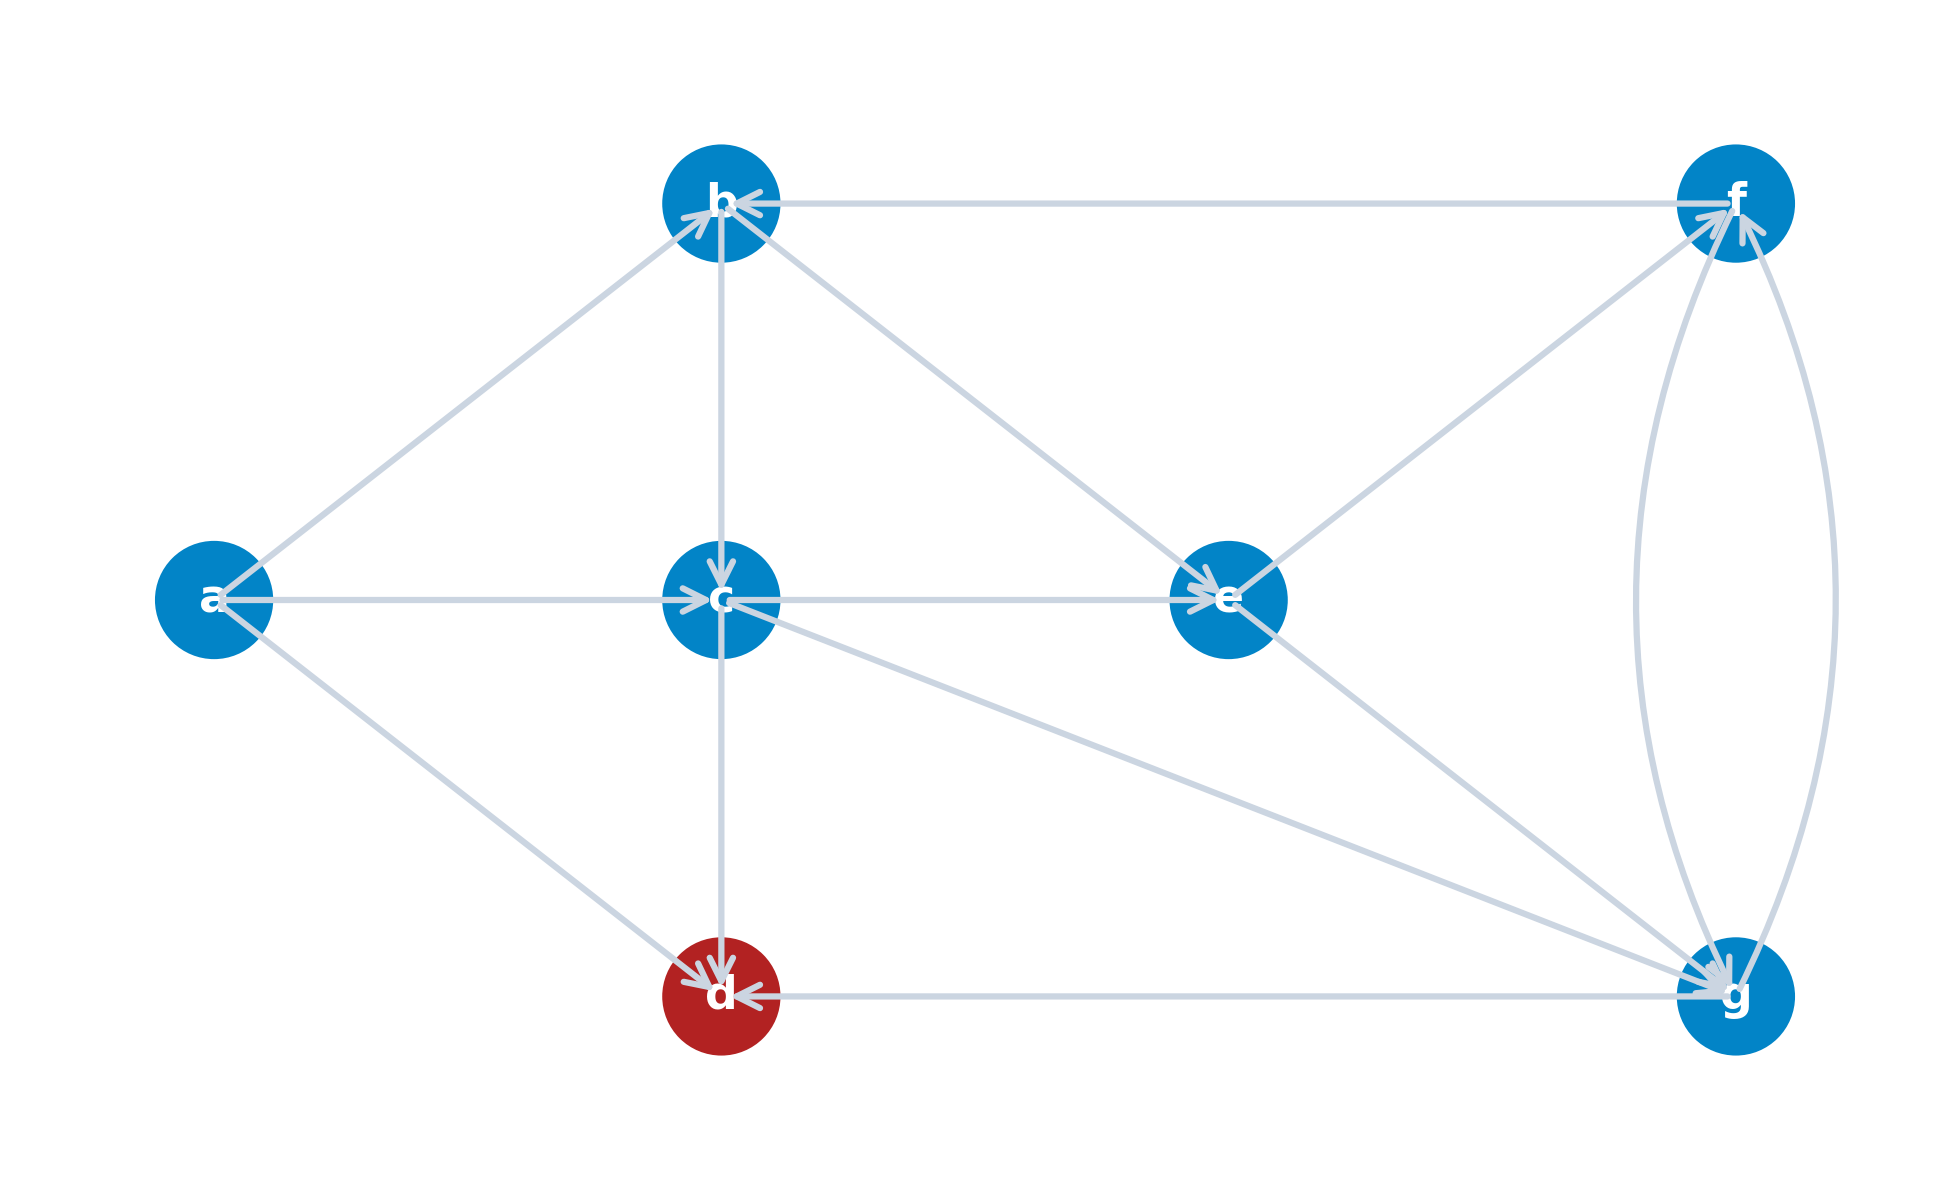
\includegraphics[keepaspectratio]{../images/digrafo_conexidad_ejemplo.png}}
\end{column}
\end{columns}
\end{frame}

\begin{frame}{Componentes conexas como relación de equivalencia}
\phantomsection\label{componentes-conexas-como-relaciuxf3n-de-equivalencia}
\begin{columns}[T]
\begin{column}{0.55\linewidth}
\begin{tcolorbox}[enhanced jigsaw, toptitle=1mm, opacityback=0, opacitybacktitle=0.6, colback=white, arc=.35mm, bottomrule=.15mm, titlerule=0mm, coltitle=black, breakable, bottomtitle=1mm, left=2mm, title=\textcolor{quarto-callout-note-color}{\faInfo}\hspace{0.5em}{Definición: Relación R de conexidad}, colbacktitle=quarto-callout-note-color!10!white, rightrule=.15mm, toprule=.15mm, colframe=quarto-callout-note-color-frame, leftrule=.75mm]

\(i \, R \, j \iff \exists \text{ cadena entre } i \text{ y } j\).

Es una \textbf{relación de equivalencia}:

\begin{enumerate}
\tightlist
\item
  \textbf{Reflexiva}: \(i \, R \, i\) (cadena de longitud 0).
\item
  \textbf{Simétrica}: \(i \, R \, j \implies j \, R \, i\).
\item
  \textbf{Transitiva}:
  \(i \, R \, j \land j \, R \, k \implies i \, R \, k\).
\end{enumerate}

Las clases de equivalencia definen las \textbf{componentes conexas}.

\end{tcolorbox}
\end{column}

\begin{column}{0.45\linewidth}
\pandocbounded{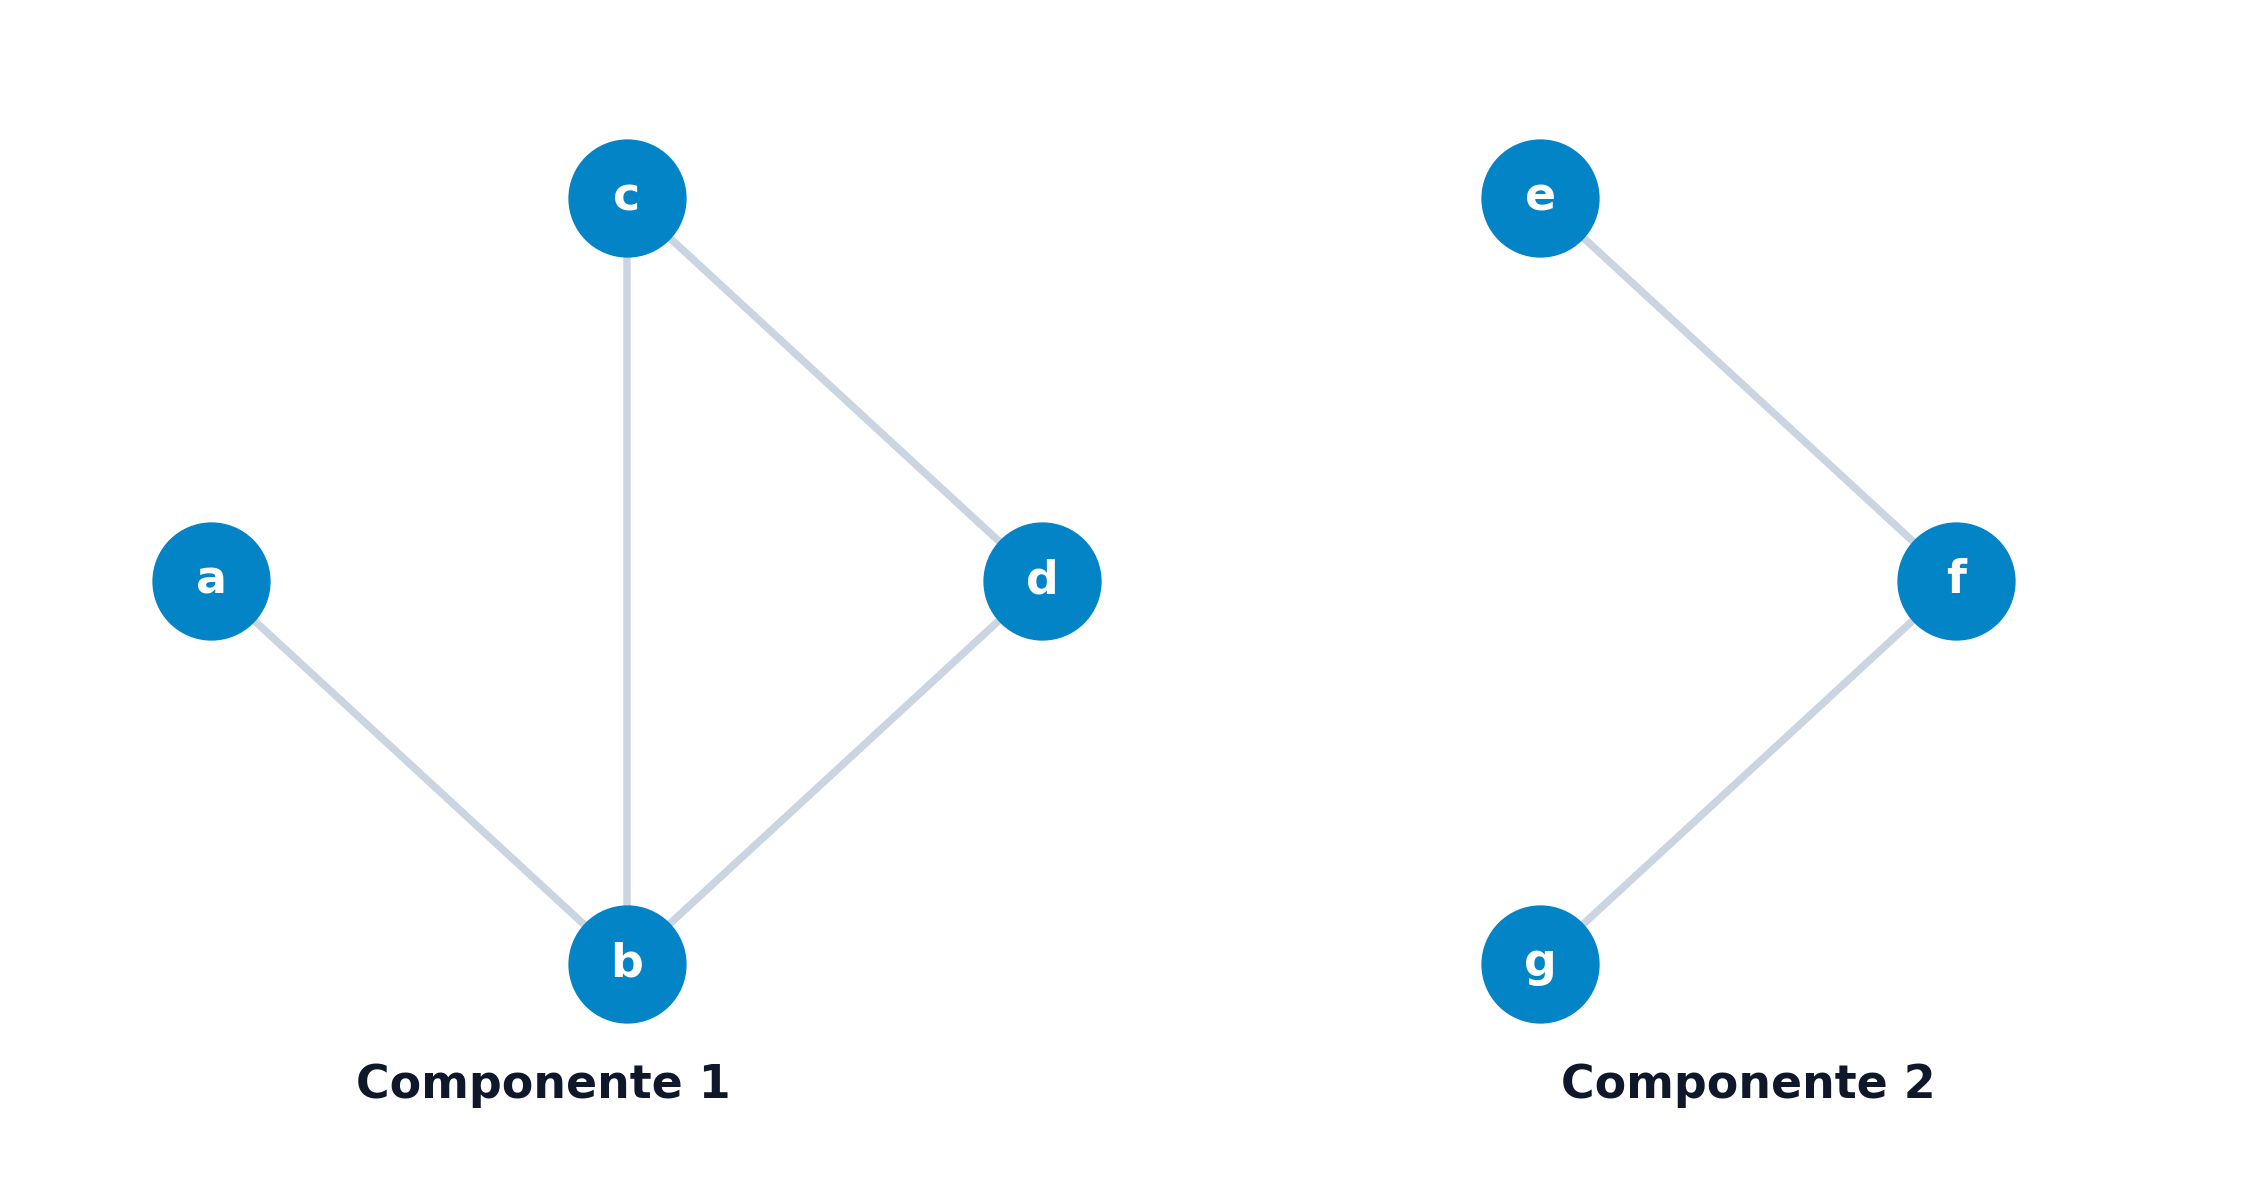
\includegraphics[keepaspectratio]{../images/componentes_conexas_dos.png}}

\begin{itemize}
\tightlist
\item
  Grafo descompuesto en 2 componentes conexas disjuntas.
\end{itemize}
\end{column}
\end{columns}
\end{frame}

\begin{frame}{Ciclos, circuitos y árboles}
\phantomsection\label{ciclos-circuitos-y-uxe1rboles}
\begin{columns}[T]
\begin{column}{0.5\linewidth}
\begin{tcolorbox}[enhanced jigsaw, toptitle=1mm, opacityback=0, opacitybacktitle=0.6, colback=white, arc=.35mm, bottomrule=.15mm, titlerule=0mm, coltitle=black, breakable, bottomtitle=1mm, left=2mm, title=\textcolor{quarto-callout-note-color}{\faInfo}\hspace{0.5em}{Definición: Recorridos cerrados}, colbacktitle=quarto-callout-note-color!10!white, rightrule=.15mm, toprule=.15mm, colframe=quarto-callout-note-color-frame, leftrule=.75mm]

\begin{itemize}
\tightlist
\item
  \textbf{Ciclo}: Cadena simple cerrada (\(v_0 = v_k\)).
\item
  \textbf{Circuito}: Camino simple cerrado (\(v_0 = v_k\)).
\item
  \textbf{Bucle}: Ciclo de un solo arco/arista \((i, i)\).
\item
  \textbf{Árbol}: Grafo conexo acíclico.
\end{itemize}

\end{tcolorbox}
\end{column}

\begin{column}{0.5\linewidth}
\pandocbounded{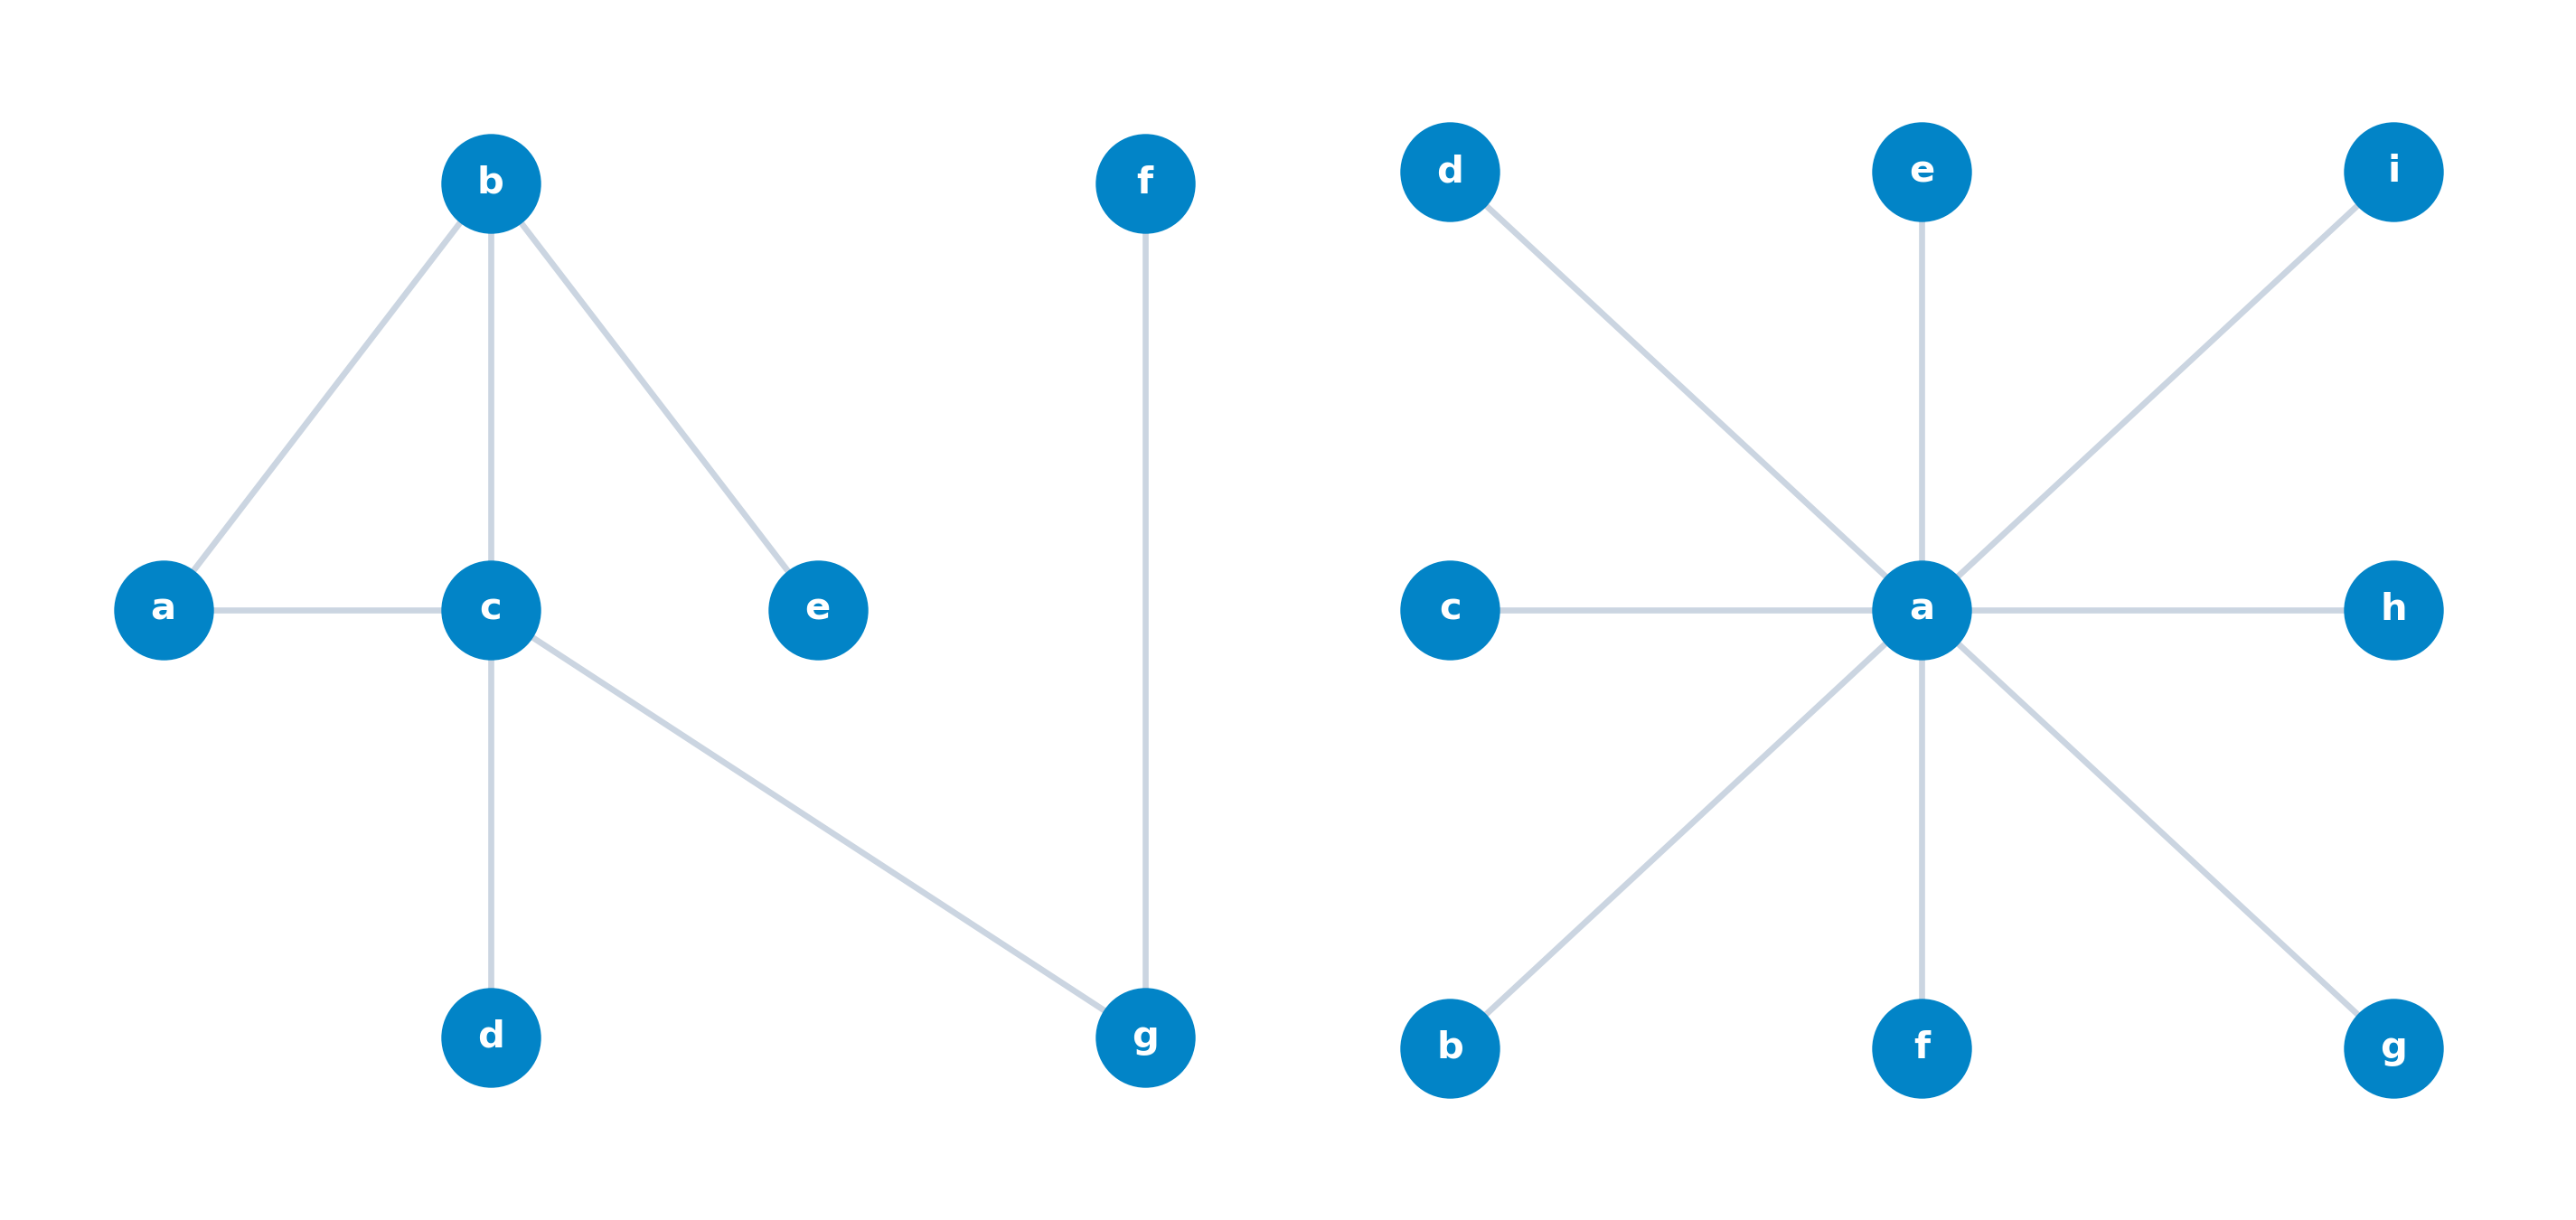
\includegraphics[keepaspectratio]{../images/arboles_ciclos_ejemplos.png}}

\begin{itemize}
\tightlist
\item
  Izquierda: Grafo con ciclo en triángulo.
\item
  Derecha: Árbol en estrella acíclico.
\end{itemize}
\end{column}
\end{columns}
\end{frame}

\begin{frame}{Teorema de estructura de ciclos y hojas}
\phantomsection\label{teorema-de-estructura-de-ciclos-y-hojas}
\begin{tcolorbox}[enhanced jigsaw, toptitle=1mm, opacityback=0, opacitybacktitle=0.6, colback=white, arc=.35mm, bottomrule=.15mm, titlerule=0mm, coltitle=black, breakable, bottomtitle=1mm, left=2mm, title=\textcolor{quarto-callout-important-color}{\faExclamation}\hspace{0.5em}{Propiedades estructurales}, colbacktitle=quarto-callout-important-color!10!white, rightrule=.15mm, toprule=.15mm, colframe=quarto-callout-important-color-frame, leftrule=.75mm]

Para todo grafo conexo \(G = (V, E)\) con \(n > 1\):

\begin{enumerate}
\tightlist
\item
  \textbf{Ausencia de hojas}: Si todos los vértices tienen grado
  \(d(v) \ge 2\), \(G\) contiene \textbf{al menos un ciclo}.
\item
  \textbf{Existencia de hojas}: Todo árbol conexo contiene \textbf{al
  menos un vértice pendiente} (hoja con \(d(v) = 1\)).
\item
  \textbf{Aristas en ciclos}: Una arista \(e\) pertenece a un ciclo si y
  solo si \(G \setminus \{e\}\) sigue siendo conexo.
\end{enumerate}

\end{tcolorbox}
\end{frame}

\section{Grafos planares y
bipartitos}\label{grafos-planares-y-bipartitos}

\begin{frame}{Grafos planares y regiones}
\phantomsection\label{grafos-planares-y-regiones}
\begin{columns}[T]
\begin{column}{0.5\linewidth}
\begin{tcolorbox}[enhanced jigsaw, toptitle=1mm, opacityback=0, opacitybacktitle=0.6, colback=white, arc=.35mm, bottomrule=.15mm, titlerule=0mm, coltitle=black, breakable, bottomtitle=1mm, left=2mm, title=\textcolor{quarto-callout-note-color}{\faInfo}\hspace{0.5em}{Definición: Grafo planar e incrustación}, colbacktitle=quarto-callout-note-color!10!white, rightrule=.15mm, toprule=.15mm, colframe=quarto-callout-note-color-frame, leftrule=.75mm]

\begin{itemize}
\tightlist
\item
  \textbf{Grafo Planar}: Admite un dibujo en \(\mathbb{R}^2\) sin
  intersecciones entre aristas.
\item
  \textbf{Incrustación planar}: Dibujo sin cruces que divide el plano en
  \(r\) \textbf{caras/regiones} (incluyendo 1 región exterior no
  acotada).
\end{itemize}

\end{tcolorbox}
\end{column}

\begin{column}{0.5\linewidth}
\pandocbounded{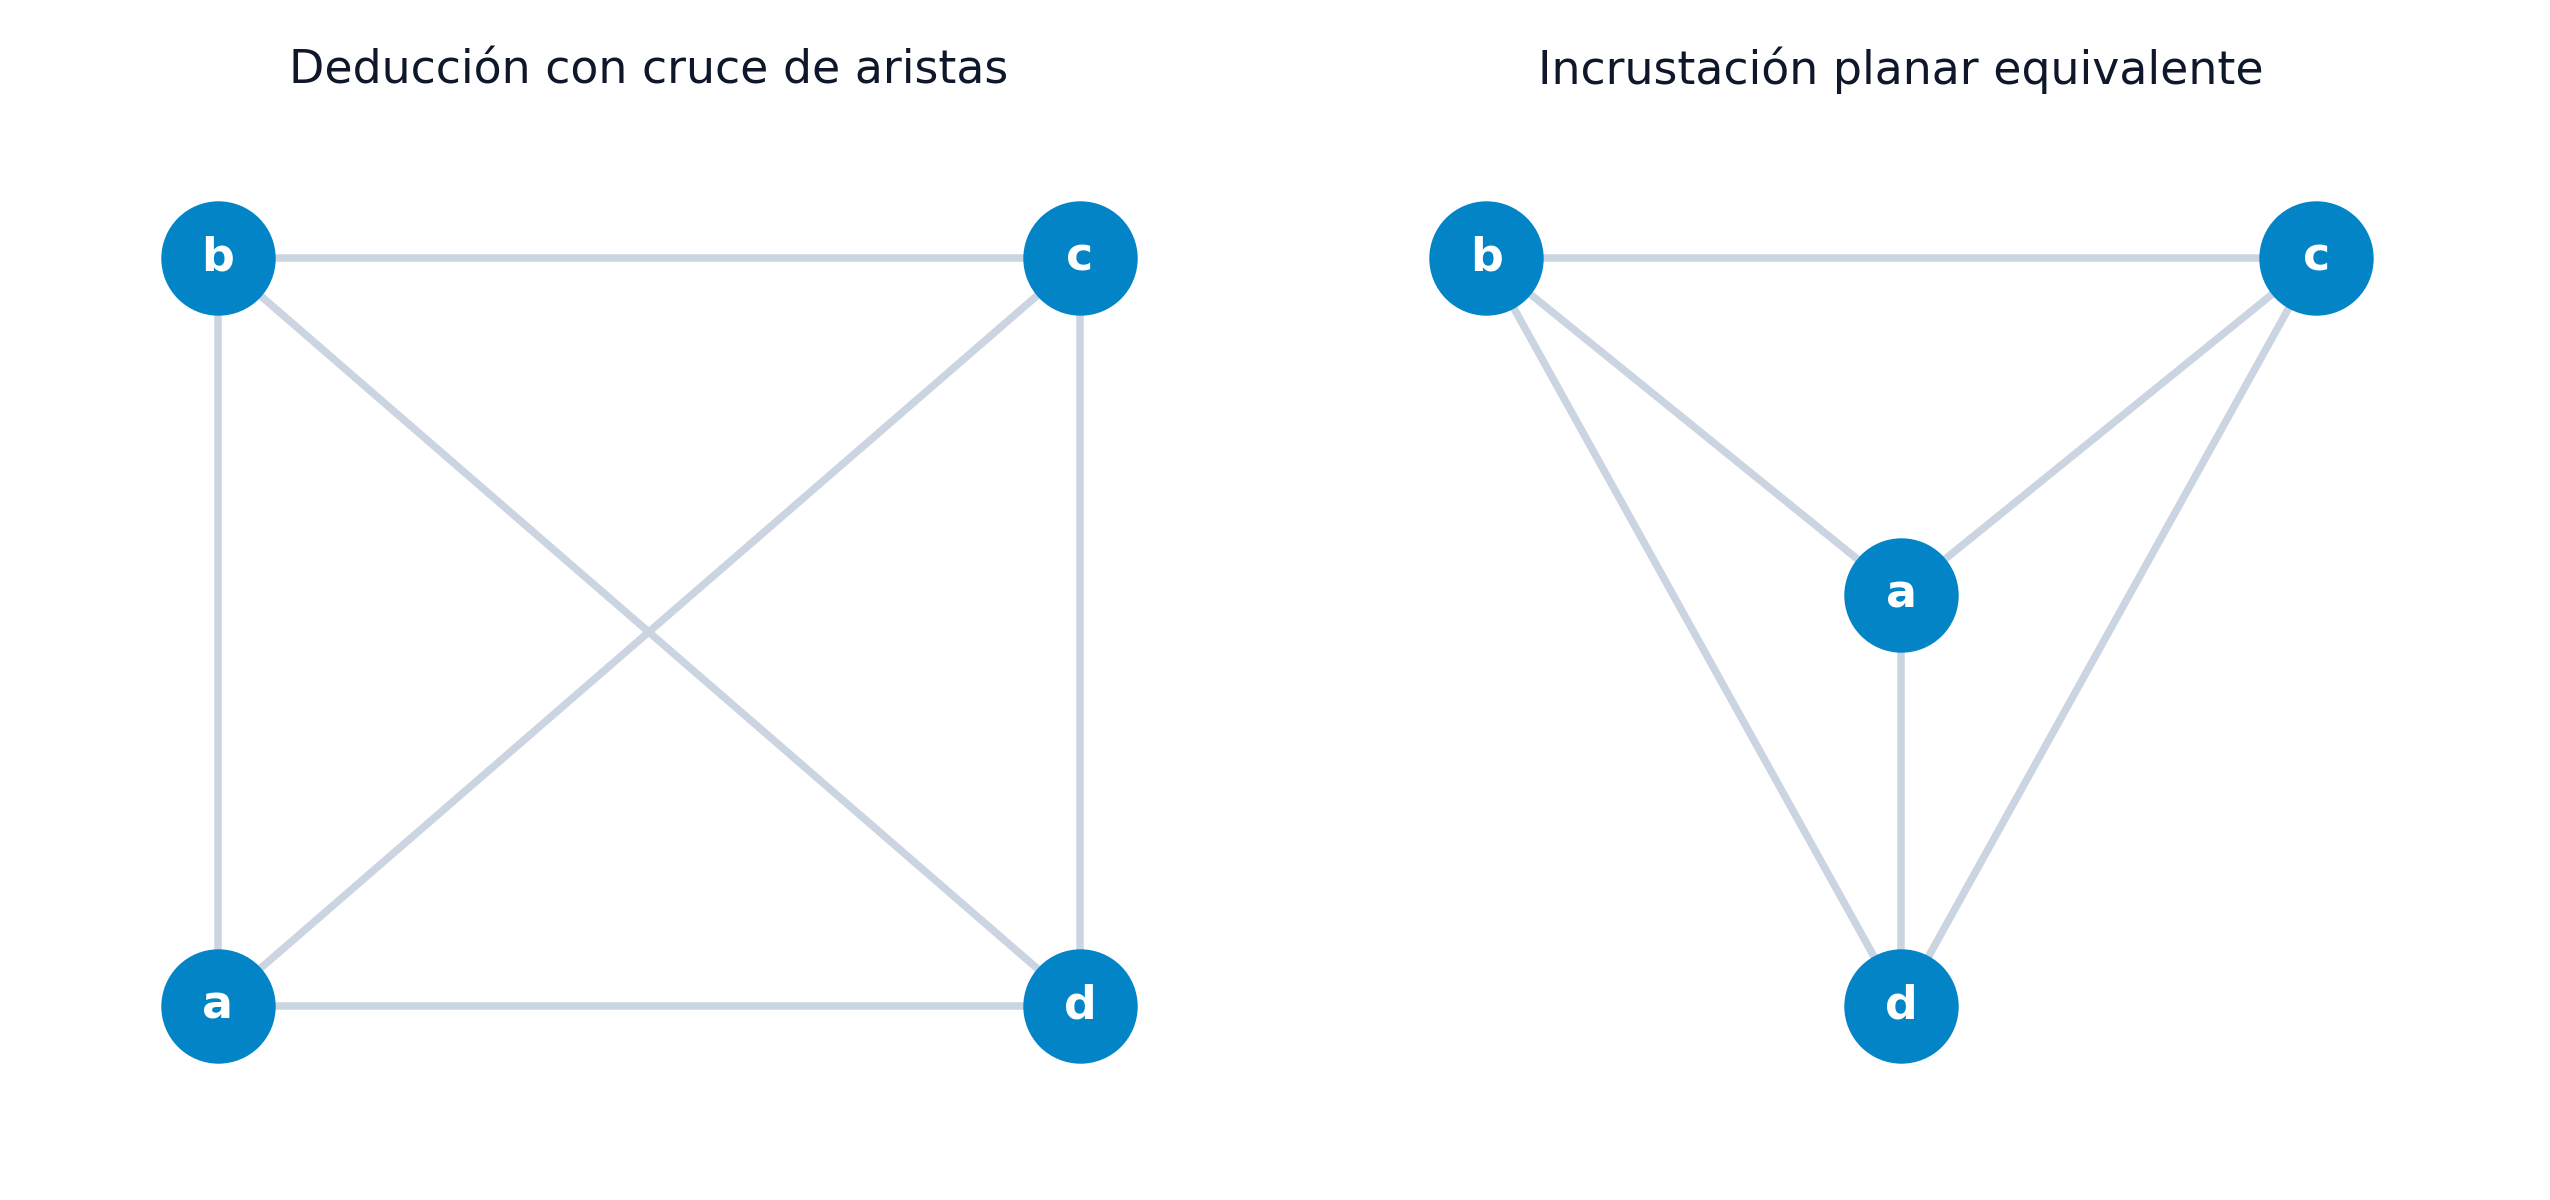
\includegraphics[keepaspectratio]{../images/k4_planaridad_ejemplo.png}}

\begin{itemize}
\tightlist
\item
  El clan \(K_4\) es \textbf{planar} al incrustar el nodo \(a\) dentro
  de la región \(\{b,c,d\}\).
\end{itemize}
\end{column}
\end{columns}
\end{frame}

\begin{frame}{Acertijo de August Möbius (1840): El Rey y sus 5 Hijos}
\phantomsection\label{acertijo-de-august-muxf6bius-1840-el-rey-y-sus-5-hijos}
\begin{tcolorbox}[enhanced jigsaw, toptitle=1mm, opacityback=0, opacitybacktitle=0.6, colback=white, arc=.35mm, bottomrule=.15mm, titlerule=0mm, coltitle=black, breakable, bottomtitle=1mm, left=2mm, title=\textcolor{quarto-callout-note-color}{\faInfo}\hspace{0.5em}{Testamento del Rey (Acertijo de August Möbius, 1840)}, colbacktitle=quarto-callout-note-color!10!white, rightrule=.15mm, toprule=.15mm, colframe=quarto-callout-note-color-frame, leftrule=.75mm]

\begin{quote}
\emph{``Un rey ordenó en su testamento que, tras su muerte, su reino
fuera dividido entre sus 5 hijos en 5 regiones contiguas de forma que
cada región tuviera frontera común con todas las demás 4 regiones. ¿Es
posible cumplir la voluntad del rey?''}
\end{quote}

\end{tcolorbox}

\begin{itemize}
\tightlist
\item
  \textbf{Pregunta fundamental}: ¿Puede existir un mapa plano dividido
  en 5 regiones adyacentes donde todas compartan frontera común con las
  otras cuatro?
\end{itemize}
\end{frame}

\begin{frame}{El Acertijo de Möbius y la no planaridad de \(K_5\)}
\phantomsection\label{el-acertijo-de-muxf6bius-y-la-no-planaridad-de-k_5}
\begin{columns}[T]
\begin{column}{0.55\linewidth}
\begin{itemize}
\tightlist
\item
  \textbf{Formulación mediante teoría de redes}:

  \begin{itemize}
  \tightlist
  \item
    Cumplir el testamento exige que el grafo dual de fronteras sea un
    \textbf{grafo completo de 5 vértices (\(K_5\))}.
  \item
    \(K_5\) integra \(n=5\) vértices y \(m = \frac{5 \times 4}{2} = 10\)
    aristas.
  \end{itemize}
\item
  \textbf{Resultado matemático}:

  \begin{itemize}
  \tightlist
  \item
    La respuesta es \textbf{negativa}.
  \item
    \(K_5\) es un \textbf{grafo no planar}: cualquier intento de
    incrustar sus 10 aristas en el plano produce al menos un cruce
    inevitable.
  \end{itemize}
\end{itemize}
\end{column}

\begin{column}{0.45\linewidth}
\pandocbounded{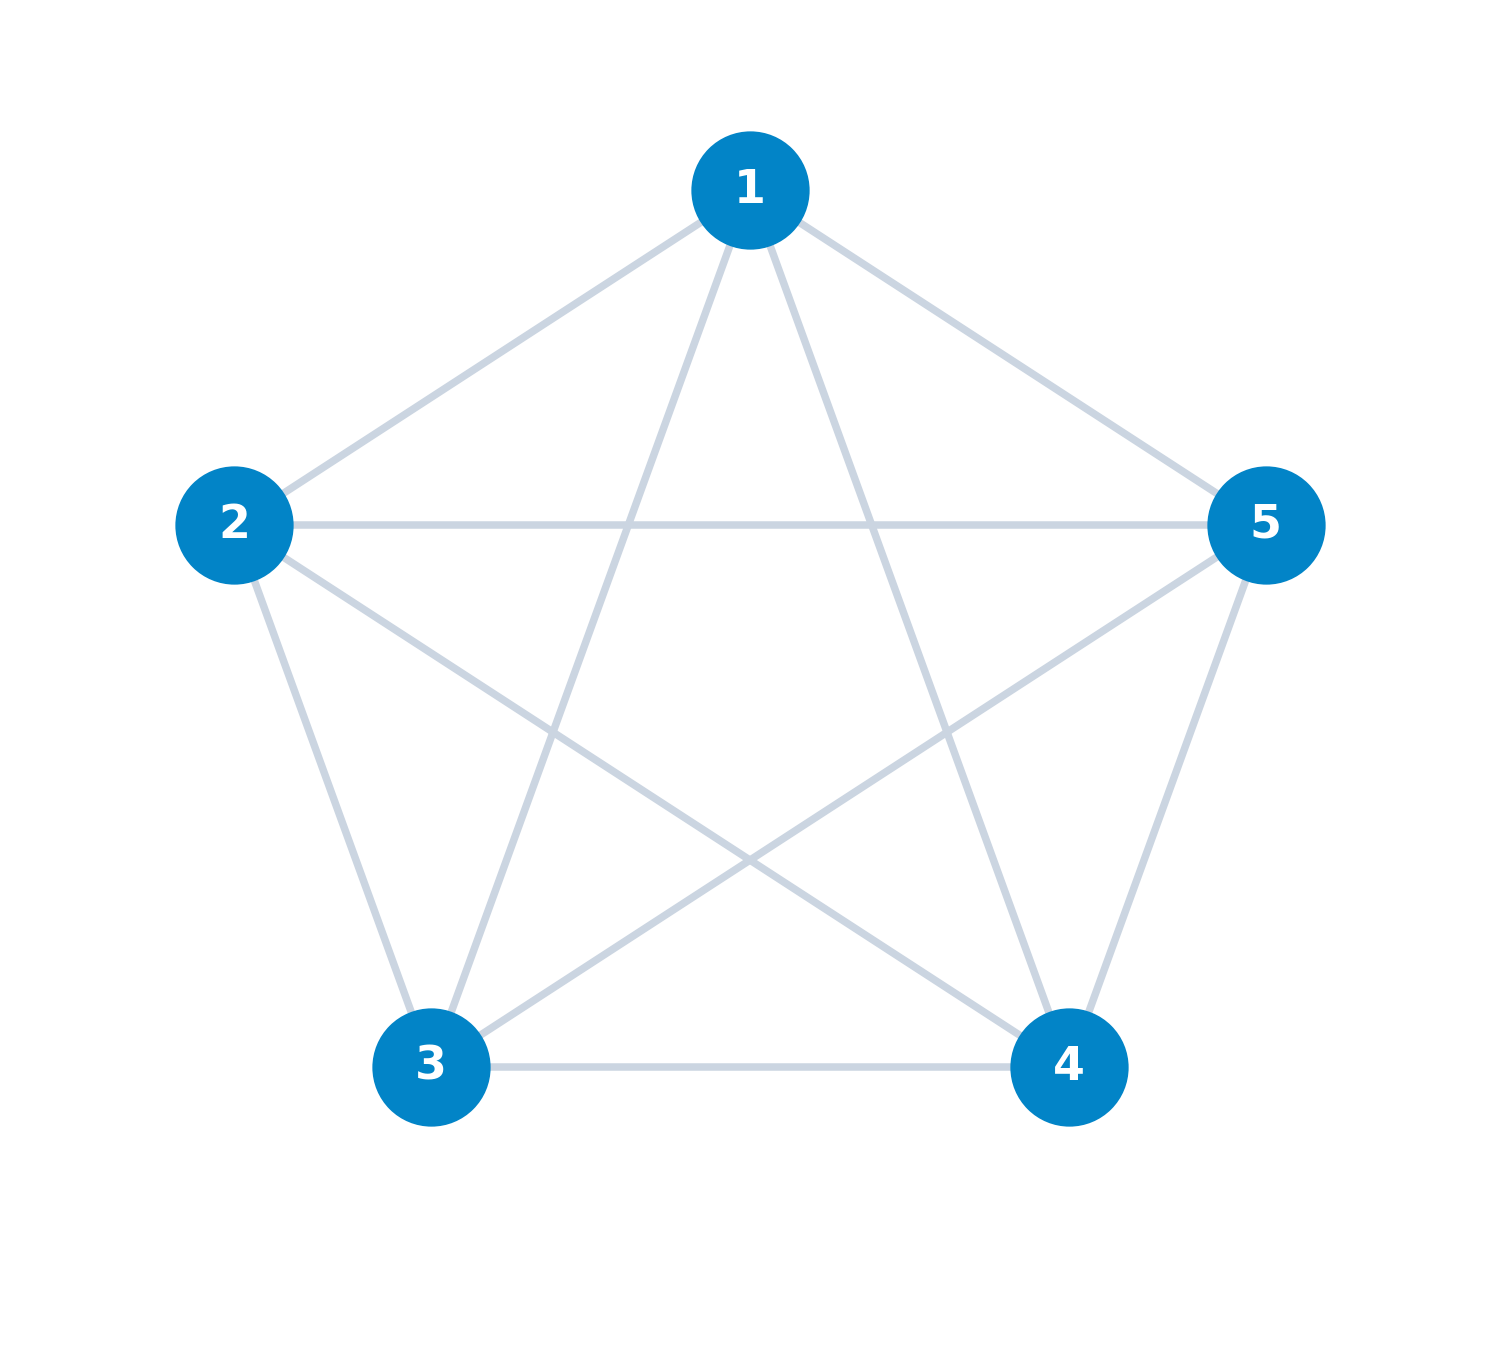
\includegraphics[keepaspectratio]{../images/k5_mobius_problema.png}}
\end{column}
\end{columns}
\end{frame}

\begin{frame}{Grafos bipartitos y Bipartitos completos}
\phantomsection\label{grafos-bipartitos-y-bipartitos-completos}
\begin{tcolorbox}[enhanced jigsaw, toptitle=1mm, opacityback=0, opacitybacktitle=0.6, colback=white, arc=.35mm, bottomrule=.15mm, titlerule=0mm, coltitle=black, breakable, bottomtitle=1mm, left=2mm, title=\textcolor{quarto-callout-note-color}{\faInfo}\hspace{0.5em}{Definición: Grafo bipartito y bipartito completo}, colbacktitle=quarto-callout-note-color!10!white, rightrule=.15mm, toprule=.15mm, colframe=quarto-callout-note-color-frame, leftrule=.75mm]

Un grafo \(G = (V, E)\) es \textbf{bipartito} si su conjunto de vértices
admite una partición en dos subconjuntos disjuntos: \[
V = V_1 \cup V_2, \quad V_1 \cap V_2 = \emptyset
\] tal que toda arista conecta un vértice de \(V_1\) con un vértice de
\(V_2\).

\begin{itemize}
\tightlist
\item
  \textbf{Bipartito Completo \(K_{n_1, n_2}\)}: Contiene todas las
  \(n_1 \cdot n_2\) aristas entre \(V_1\) y \(V_2\).
\end{itemize}

\end{tcolorbox}

\begin{tcolorbox}[enhanced jigsaw, toptitle=1mm, opacityback=0, opacitybacktitle=0.6, colback=white, arc=.35mm, bottomrule=.15mm, titlerule=0mm, coltitle=black, breakable, bottomtitle=1mm, left=2mm, title=\textcolor{quarto-callout-important-color}{\faExclamation}\hspace{0.5em}{Caracterización}, colbacktitle=quarto-callout-important-color!10!white, rightrule=.15mm, toprule=.15mm, colframe=quarto-callout-important-color-frame, leftrule=.75mm]

Un grafo es bipartito \(\iff\) \textbf{no contiene ningún ciclo de
longitud impar}.

\end{tcolorbox}
\end{frame}

\begin{frame}{Problema de los tres servicios de Dudeney (1917)}
\phantomsection\label{problema-de-los-tres-servicios-de-dudeney-1917}
\begin{tcolorbox}[enhanced jigsaw, toptitle=1mm, opacityback=0, opacitybacktitle=0.6, colback=white, arc=.35mm, bottomrule=.15mm, titlerule=0mm, coltitle=black, breakable, bottomtitle=1mm, left=2mm, title=\textcolor{quarto-callout-note-color}{\faInfo}\hspace{0.5em}{Acertijo de Henry Ernest Dudeney (1917)}, colbacktitle=quarto-callout-note-color!10!white, rightrule=.15mm, toprule=.15mm, colframe=quarto-callout-note-color-frame, leftrule=.75mm]

\begin{quote}
\emph{``¿Es posible canalizar las conducciones subterráneas de tres
suministros esenciales (agua, gas y electricidad) hacia tres viviendas
independientes de modo que ninguna tubería o cable se cruce con otro en
el plano?''}
\end{quote}

\end{tcolorbox}

\begin{itemize}
\tightlist
\item
  \textbf{Pregunta fundamental}: ¿Es posible conectar 3 fuentes de
  suministro (\(A, G, E\)) a 3 casas (\(C_1, C_2, C_3\)) sin que los
  tendidos de tuberías o cables se intercepten en el plano?
\end{itemize}
\end{frame}

\begin{frame}{El Problema de Dudeney y la no planaridad de \(K_{3,3}\)}
\phantomsection\label{el-problema-de-dudeney-y-la-no-planaridad-de-k_33}
\begin{columns}[T]
\begin{column}{0.55\linewidth}
\begin{itemize}
\tightlist
\item
  \textbf{Formulación mediante teoría de redes}:

  \begin{itemize}
  \tightlist
  \item
    Modela la incrustación del \textbf{grafo bipartito completo
    \(K_{3,3}\)} (\(n_1=3\) suministros, \(n_2=3\) casas,
    \(m = 3 \times 3 = 9\) aristas).
  \end{itemize}
\item
  \textbf{Resultado matemático}:

  \begin{itemize}
  \tightlist
  \item
    La respuesta al acertijo es \textbf{negativa}.
  \item
    \(K_{3,3}\) es un \textbf{grafo no planar}: tras trazar 8
    conducciones, la novena queda atrapada en una cara acotada sin poder
    completarse sin cruzar una tubería previa.
  \end{itemize}
\end{itemize}
\end{column}

\begin{column}{0.45\linewidth}
\pandocbounded{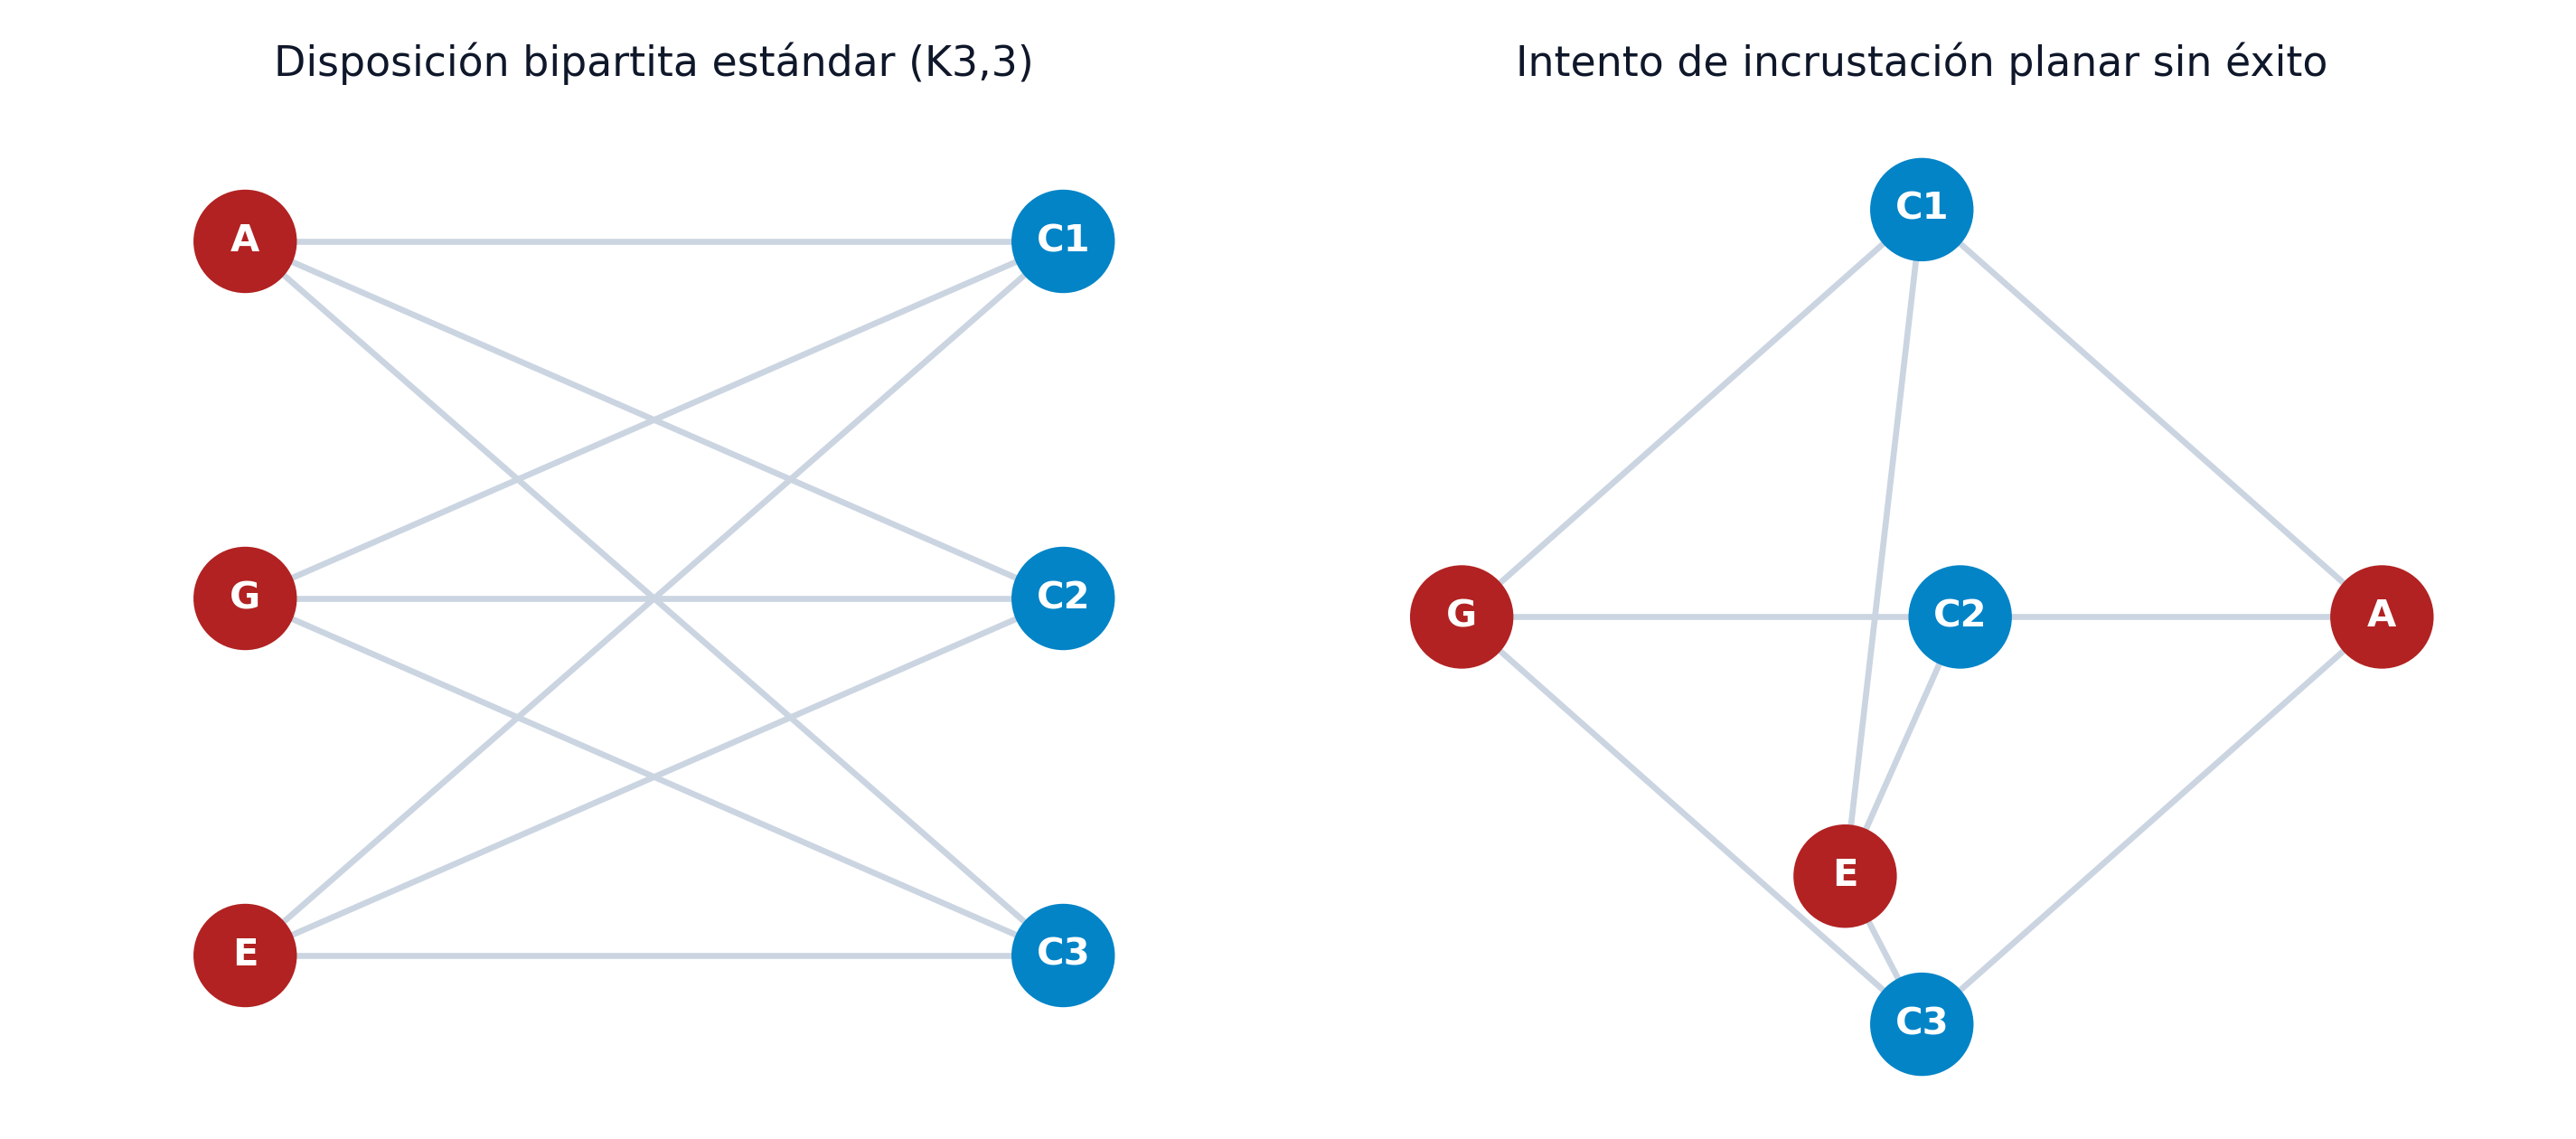
\includegraphics[keepaspectratio]{../images/k33_bipartito_dudeney.png}}
\end{column}
\end{columns}
\end{frame}

\begin{frame}{Homeomorfismo y Teorema de Kuratowski (1930)}
\phantomsection\label{homeomorfismo-y-teorema-de-kuratowski-1930}
\begin{columns}[T]
\begin{column}{0.5\linewidth}
\begin{tcolorbox}[enhanced jigsaw, toptitle=1mm, opacityback=0, opacitybacktitle=0.6, colback=white, arc=.35mm, bottomrule=.15mm, titlerule=0mm, coltitle=black, breakable, bottomtitle=1mm, left=2mm, title=\textcolor{quarto-callout-note-color}{\faInfo}\hspace{0.5em}{Definición: Homeomorfismo}, colbacktitle=quarto-callout-note-color!10!white, rightrule=.15mm, toprule=.15mm, colframe=quarto-callout-note-color-frame, leftrule=.75mm]

Dos grafos son \textbf{homeomórficos} si se obtienen uno del otro
mediante subdivisión elemental de aristas (insertar/suprimir nodos de
grado 2).

\end{tcolorbox}

\begin{tcolorbox}[enhanced jigsaw, toptitle=1mm, opacityback=0, opacitybacktitle=0.6, colback=white, arc=.35mm, bottomrule=.15mm, titlerule=0mm, coltitle=black, breakable, bottomtitle=1mm, left=2mm, title=\textcolor{quarto-callout-important-color}{\faExclamation}\hspace{0.5em}{Teorema de Kuratowski (1930)}, colbacktitle=quarto-callout-important-color!10!white, rightrule=.15mm, toprule=.15mm, colframe=quarto-callout-important-color-frame, leftrule=.75mm]

Un grafo \(G\) es \textbf{planar} \(\iff\) \textbf{no contiene ningún
subgrafo homeomórfico a \(K_5\) ni a \(K_{3,3}\)}.

\end{tcolorbox}
\end{column}

\begin{column}{0.5\linewidth}
\pandocbounded{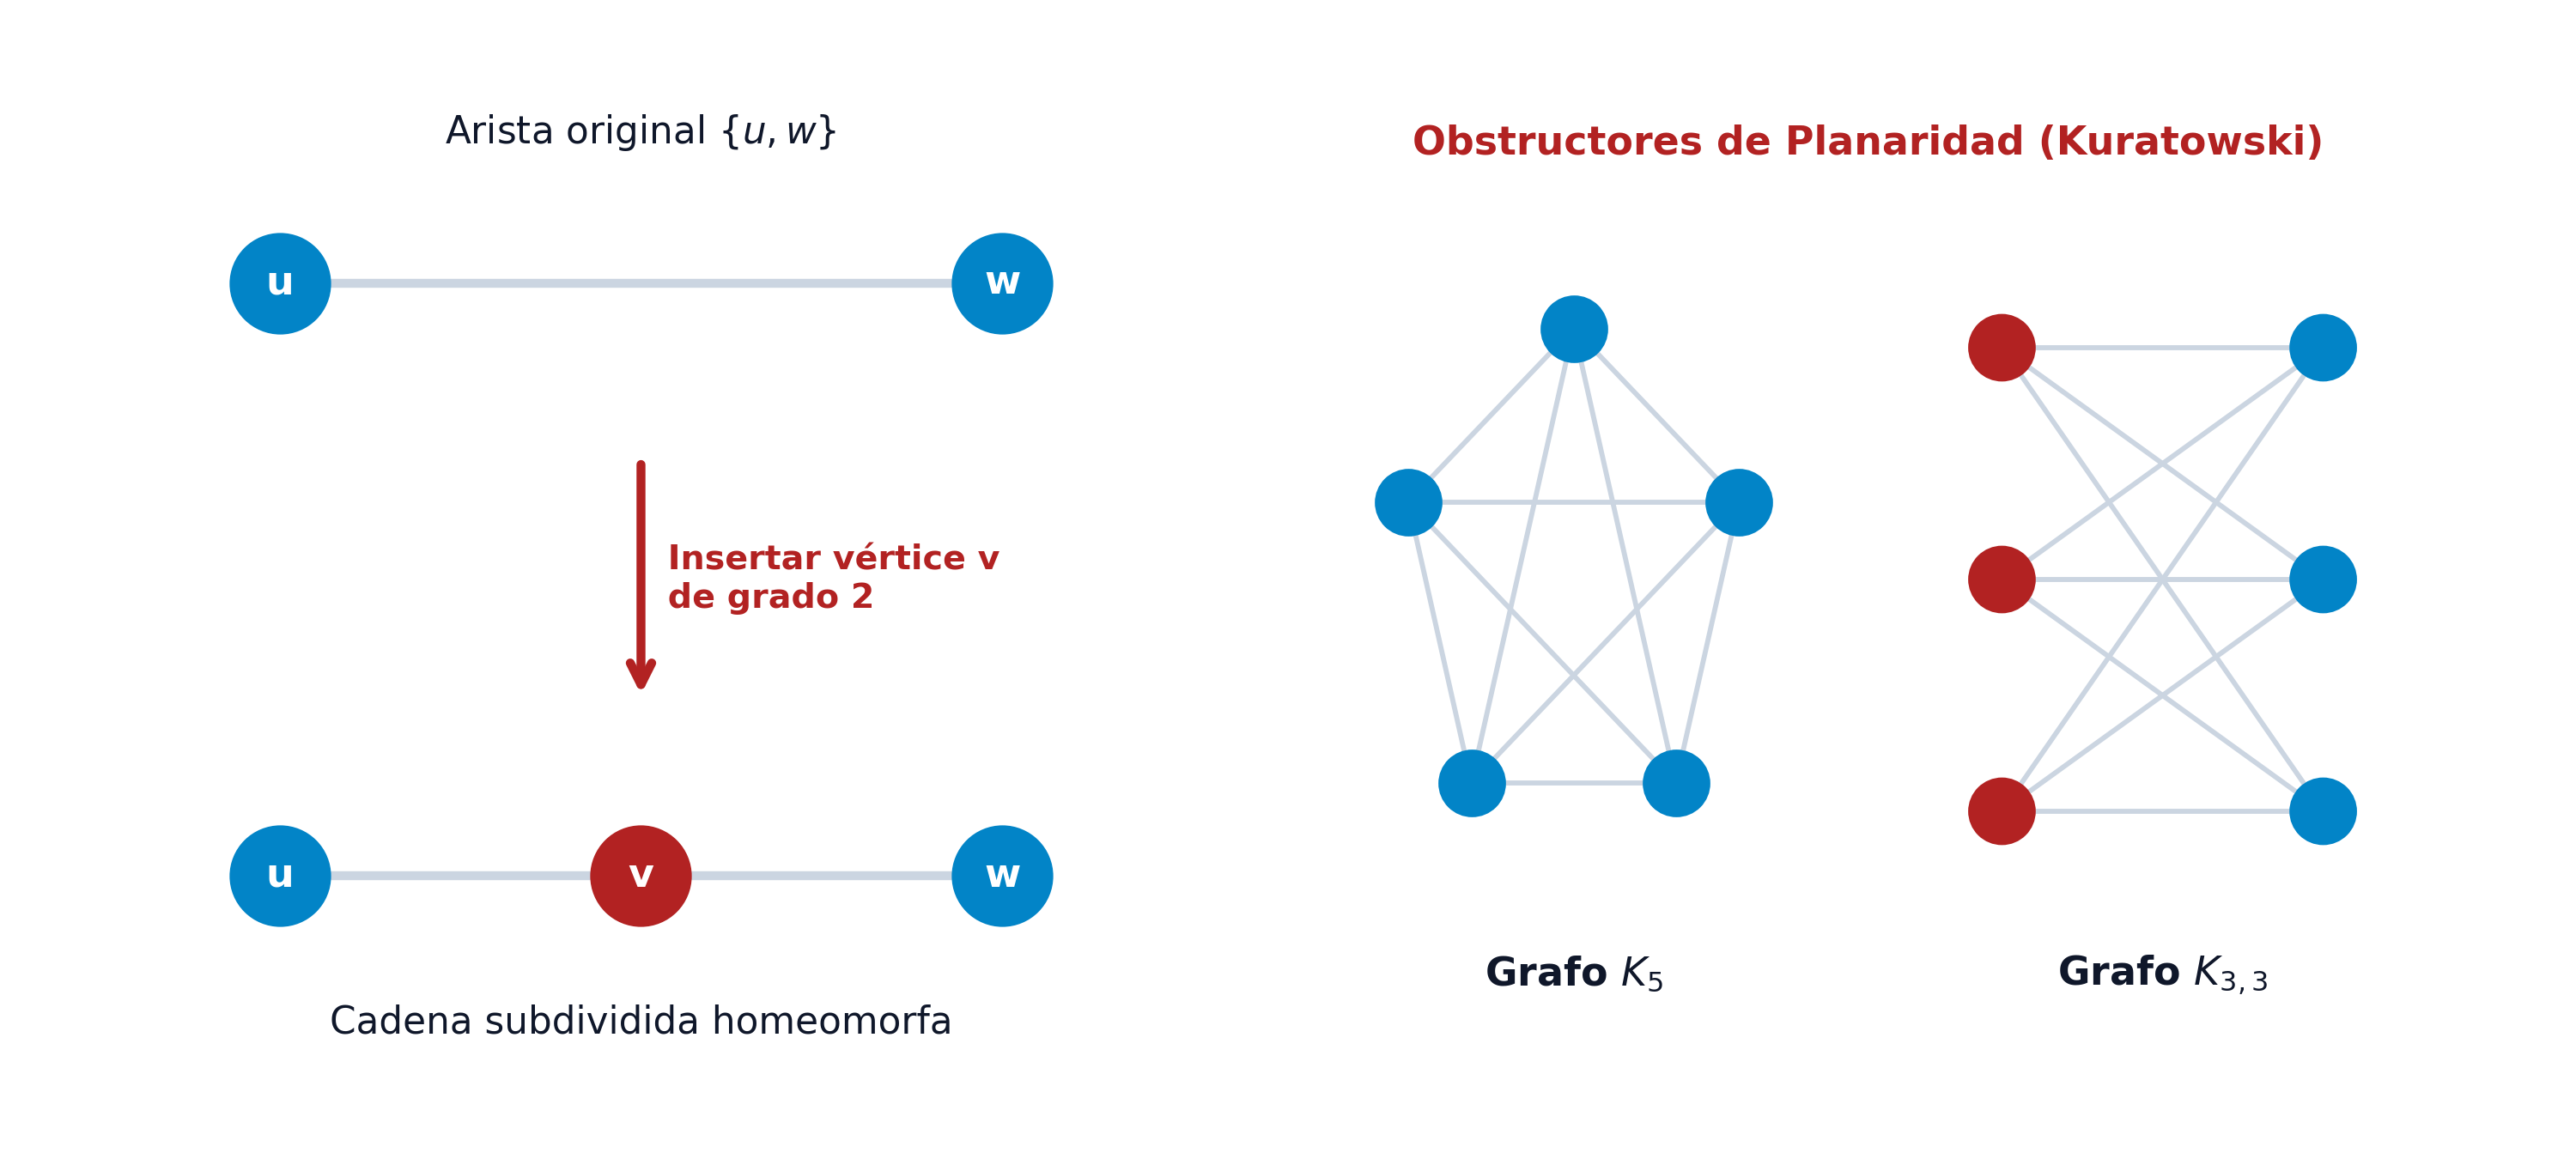
\includegraphics[keepaspectratio]{../images/kuratowski_homeomorfismo.png}}
\end{column}
\end{columns}
\end{frame}

\begin{frame}{Demostración: Grafo de Petersen}
\phantomsection\label{demostraciuxf3n-grafo-de-petersen}
\begin{columns}[T]
\begin{column}{0.5\linewidth}
\begin{itemize}
\tightlist
\item
  \textbf{Grafo de Petersen}: Grafo 3-regular con 10 vértices y 15
  aristas.
\item
  \textbf{No planaridad}: Contiene un subgrafo parcial homeomórfico a
  \(K_{3,3}\).
\item
  \textbf{Subdivisión}: Nodos rojos \(V_1 = \{j, a, d\}\), nodos azules
  \(V_2 = \{e, f, b\}\). Vértices \(g, h, i, c\) actúan de grado 2.
\end{itemize}
\end{column}

\begin{column}{0.5\linewidth}
\pandocbounded{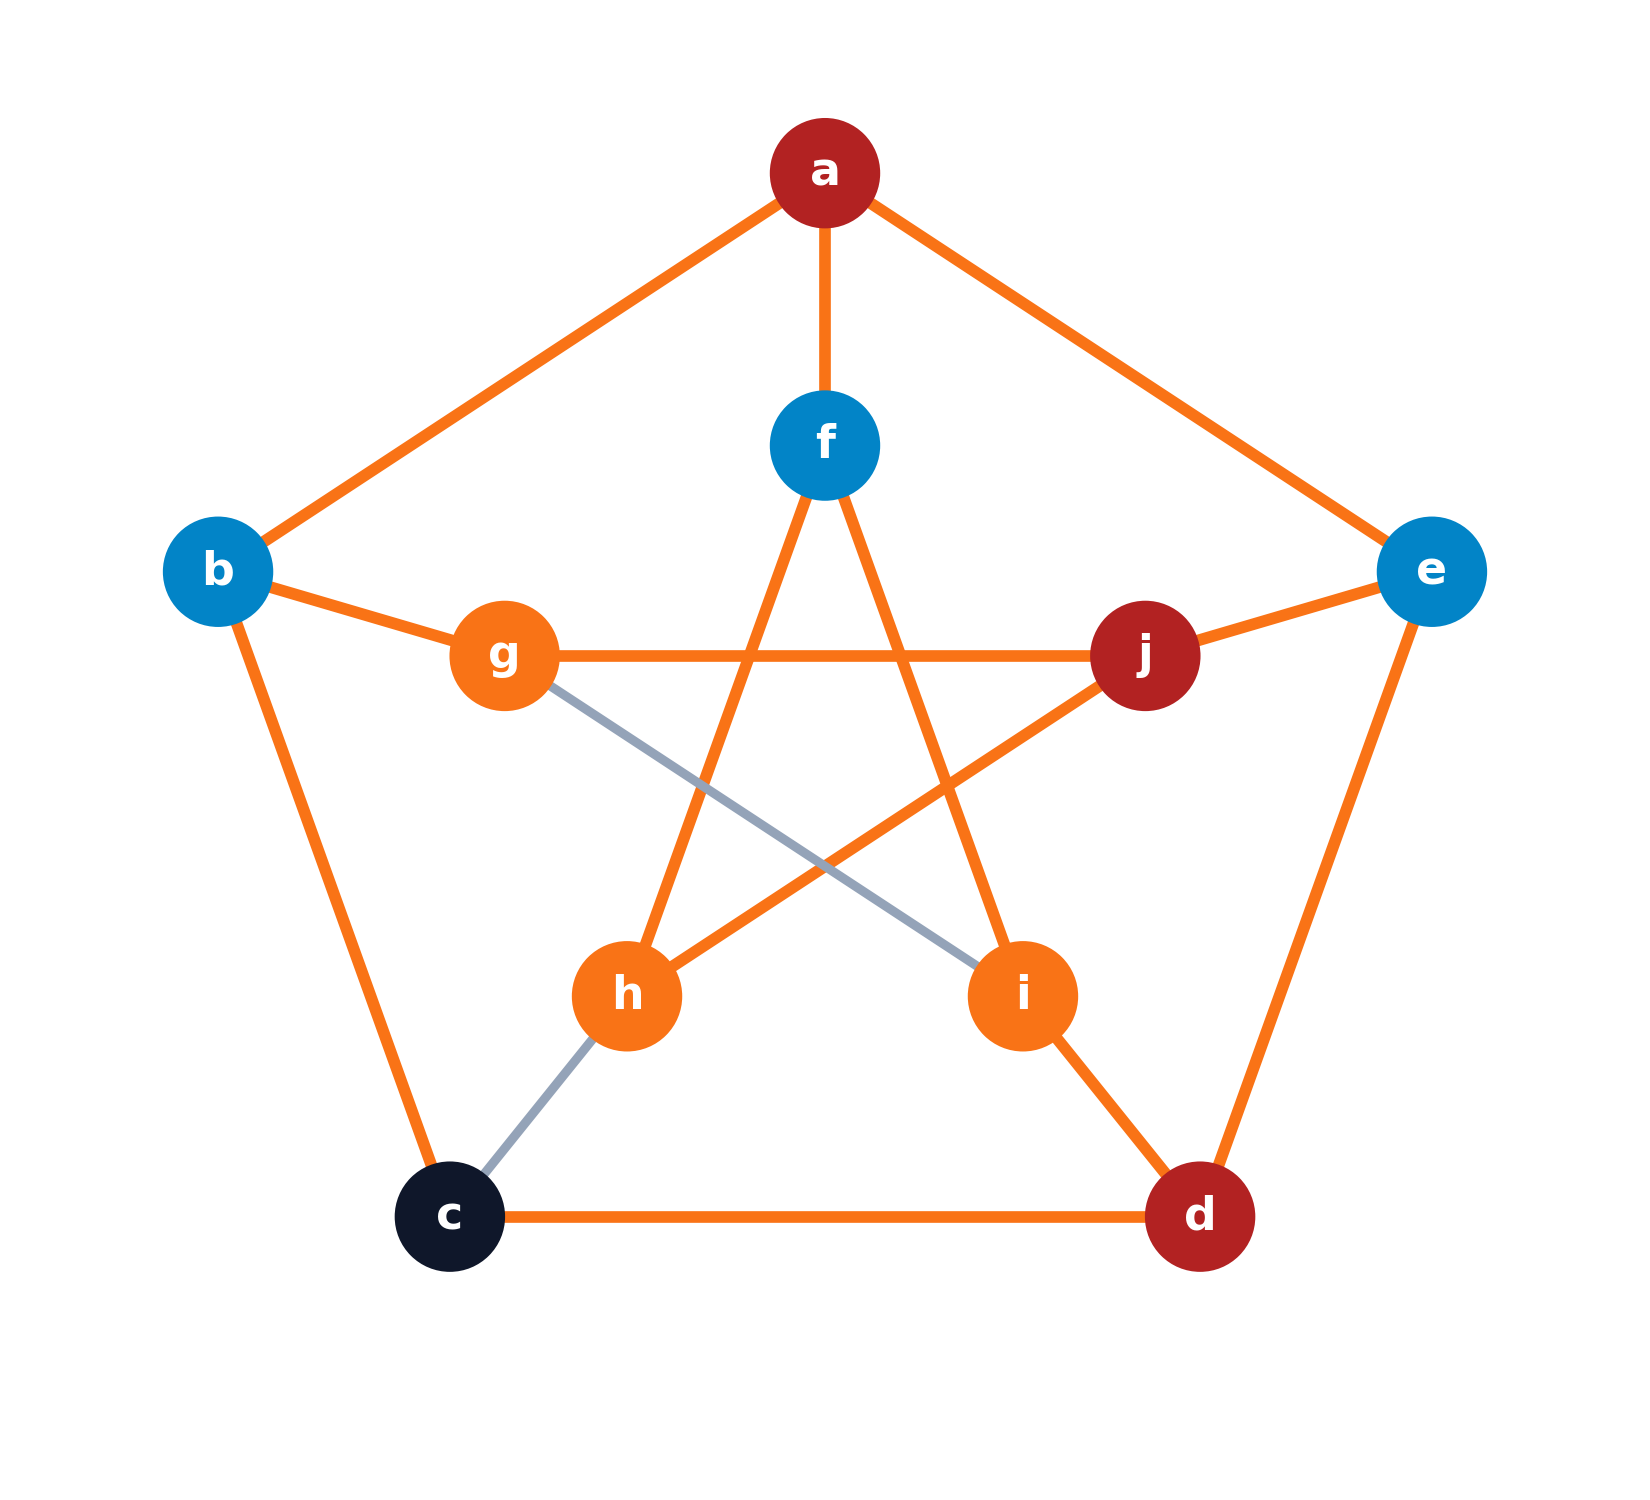
\includegraphics[keepaspectratio]{../images/petersen_k33_homeomorfismo.png}}
\end{column}
\end{columns}
\end{frame}

\begin{frame}{Fórmula planar de Euler}
\phantomsection\label{fuxf3rmula-planar-de-euler}
\begin{columns}[T]
\begin{column}{0.6\linewidth}
\begin{tcolorbox}[enhanced jigsaw, toptitle=1mm, opacityback=0, opacitybacktitle=0.6, colback=white, arc=.35mm, bottomrule=.15mm, titlerule=0mm, coltitle=black, breakable, bottomtitle=1mm, left=2mm, title=\textcolor{quarto-callout-important-color}{\faExclamation}\hspace{0.5em}{Fórmula planar de Euler}, colbacktitle=quarto-callout-important-color!10!white, rightrule=.15mm, toprule=.15mm, colframe=quarto-callout-important-color-frame, leftrule=.75mm]

En todo grafo planar conexo con \(n\) vértices, \(m\) aristas y \(r\)
regiones (incluyendo la cara exterior no acotada): \[
n + r = m + 2
\]

\end{tcolorbox}
\end{column}

\begin{column}{0.4\linewidth}
\begin{itemize}
\tightlist
\item
  \textbf{Significado geométrico}:

  \begin{itemize}
  \tightlist
  \item
    Relación invariante entre vértices, aristas y caras sobre la
    superficie del plano.
  \item
    Permite deducir las cotas superiores absolutas sobre la densidad de
    aristas en grafos planares.
  \end{itemize}
\end{itemize}
\end{column}
\end{columns}
\end{frame}

\begin{frame}{Corolarios de la Fórmula de Euler}
\phantomsection\label{corolarios-de-la-fuxf3rmula-de-euler}
\begin{tcolorbox}[enhanced jigsaw, toptitle=1mm, opacityback=0, opacitybacktitle=0.6, colback=white, arc=.35mm, bottomrule=.15mm, titlerule=0mm, coltitle=black, breakable, bottomtitle=1mm, left=2mm, title=\textcolor{quarto-callout-note-color}{\faInfo}\hspace{0.5em}{Corolario: Desigualdades de planaridad}, colbacktitle=quarto-callout-note-color!10!white, rightrule=.15mm, toprule=.15mm, colframe=quarto-callout-note-color-frame, leftrule=.75mm]

\begin{enumerate}
\tightlist
\item
  En todo grafo planar conexo simple con \(n \ge 3\): \[
  m \le 3n - 6
  \]
\item
  En todo grafo planar conexo simple \textbf{bipartito} (sin
  triángulos): \[
  m \le 2n - 4
  \]
\end{enumerate}

\end{tcolorbox}
\end{frame}

\begin{frame}{Ejemplo: Prueba analítica de no planaridad}
\phantomsection\label{ejemplo-prueba-analuxedtica-de-no-planaridad}
\begin{columns}[T]
\begin{column}{0.5\linewidth}
\begin{itemize}
\tightlist
\item
  \textbf{Prueba para \(K_5\) (\(n=5, m=10\))}:

  \begin{itemize}
  \tightlist
  \item
    Condición de planaridad para \(n \ge 3\): \[m \le 3n - 6\]
  \item
    Evaluación: \[10 \le 3(5) - 6 = 9 \quad \text{(FALSO)}\]
  \item
    \textbf{Conclusión}: \(K_5\) es \textbf{no planar}.
  \end{itemize}
\end{itemize}
\end{column}

\begin{column}{0.5\linewidth}
\begin{itemize}
\tightlist
\item
  \textbf{Prueba para \(K_{3,3}\) (\(n=6, m=9\))}:

  \begin{itemize}
  \tightlist
  \item
    Grafo bipartito sin triángulos: \[m \le 2n - 4\]
  \item
    Evaluación: \[9 \le 2(6) - 4 = 8 \quad \text{(FALSO)}\]
  \item
    \textbf{Conclusión}: \(K_{3,3}\) es \textbf{no planar}.
  \end{itemize}
\end{itemize}
\end{column}
\end{columns}
\end{frame}

\section{Representación de grafos}\label{representaciuxf3n-de-grafos}

\begin{frame}{Matriz de incidencia (Grafo no dirigido)}
\phantomsection\label{matriz-de-incidencia-grafo-no-dirigido}
\begin{columns}[T]
\begin{column}{0.58\linewidth}
\begin{tcolorbox}[enhanced jigsaw, toptitle=1mm, opacityback=0, opacitybacktitle=0.6, colback=white, arc=.35mm, bottomrule=.15mm, titlerule=0mm, coltitle=black, breakable, bottomtitle=1mm, left=2mm, title=\textcolor{quarto-callout-note-color}{\faInfo}\hspace{0.5em}{Definición: Matriz de incidencia nodo-arista}, colbacktitle=quarto-callout-note-color!10!white, rightrule=.15mm, toprule=.15mm, colframe=quarto-callout-note-color-frame, leftrule=.75mm]

Dada una red no dirigida \(G = (V, E)\), la \textbf{matriz de
incidencia} \(A \in \mathbb{R}^{n \times m}\) se define como: \[
\small
a_{ik} = \begin{cases} 
1 & \text{si } i \text{ es extremo de arista } e_k \\
0 & \text{en otro caso}
\end{cases}
\]

\end{tcolorbox}
\end{column}

\begin{column}{0.42\linewidth}
\begin{center}
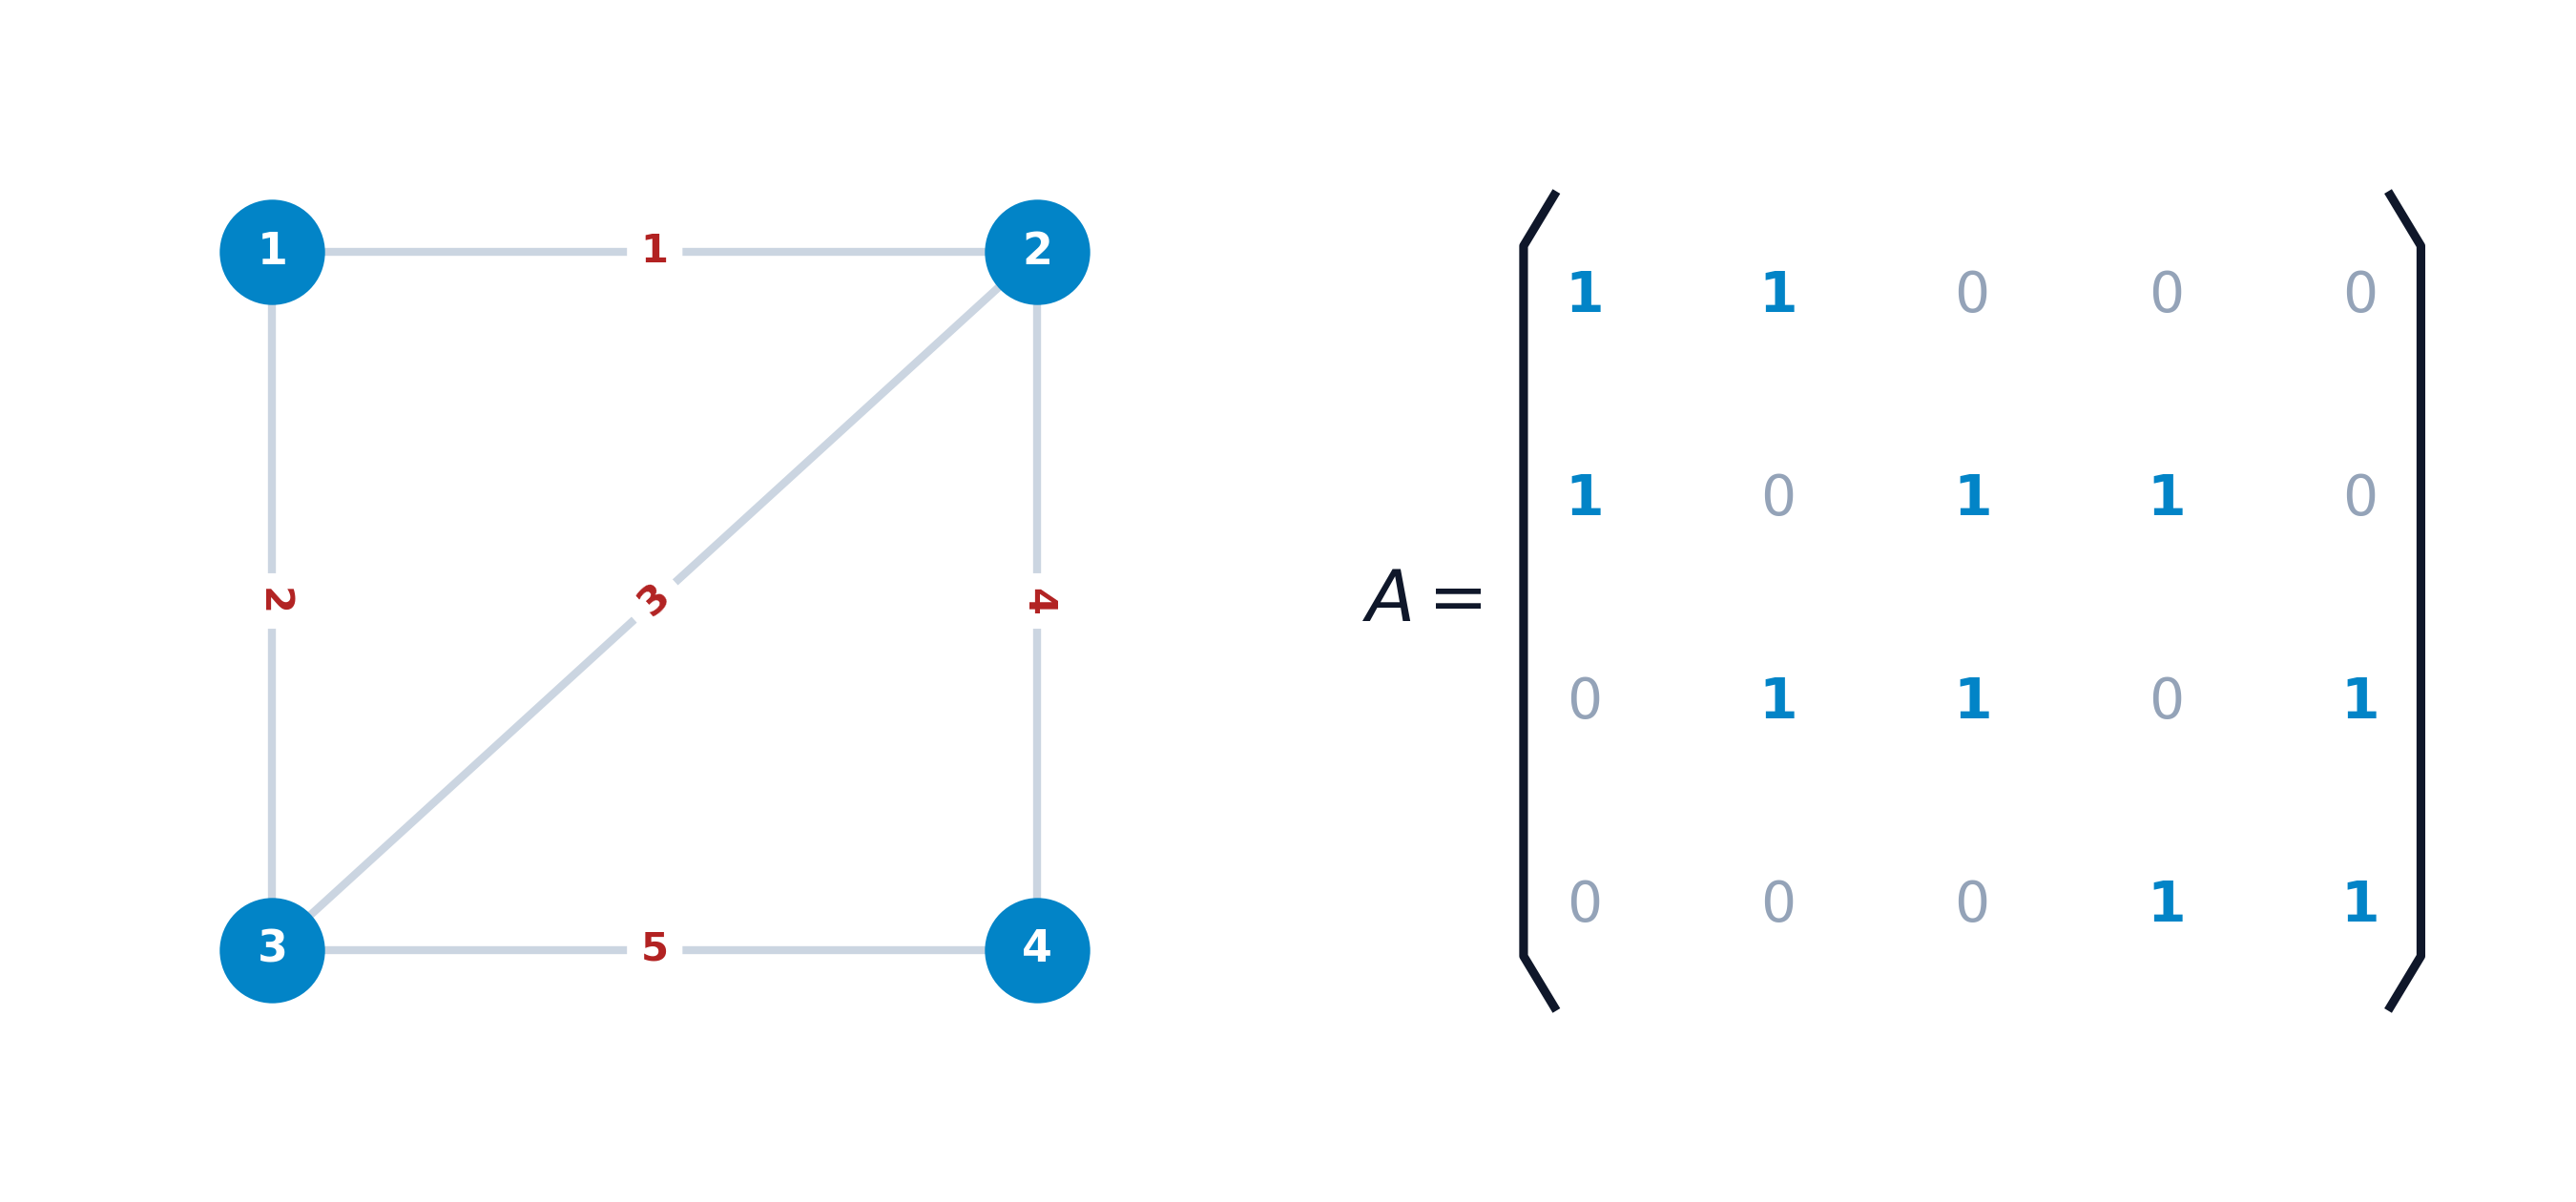
\includegraphics[width=0.9\linewidth,height=\textheight,keepaspectratio]{../images/matriz_incidencia_grafo.png}
\end{center}
\end{column}
\end{columns}

\begin{itemize}
\tightlist
\item
  \textbf{Suma por columnas}: Toda columna de \(A\) suma exactamente
  \(2\) (cada arista posee \(2\) extremos).
\end{itemize}
\end{frame}

\begin{frame}{Matriz de incidencia (Digrafo y TUM)}
\phantomsection\label{matriz-de-incidencia-digrafo-y-tum}
\begin{columns}[T]
\begin{column}{0.58\linewidth}
\begin{tcolorbox}[enhanced jigsaw, toptitle=1mm, opacityback=0, opacitybacktitle=0.6, colback=white, arc=.35mm, bottomrule=.15mm, titlerule=0mm, coltitle=black, breakable, bottomtitle=1mm, left=2mm, title=\textcolor{quarto-callout-note-color}{\faInfo}\hspace{0.5em}{Definición: Matriz de incidencia nodo-arco}, colbacktitle=quarto-callout-note-color!10!white, rightrule=.15mm, toprule=.15mm, colframe=quarto-callout-note-color-frame, leftrule=.75mm]

Dado un digrafo \(G = (V, U)\), la matriz
\(A \in \mathbb{R}^{n \times m}\) registra la orientación: \[
\small
a_{ik} = \begin{cases} 
+1 & \text{si } i \text{ es el origen del arco } u_k \\
-1 & \text{si } i \text{ es el destino del arco } u_k \\
0 & \text{en otro caso}
\end{cases}
\]

\end{tcolorbox}
\end{column}

\begin{column}{0.42\linewidth}
\begin{center}
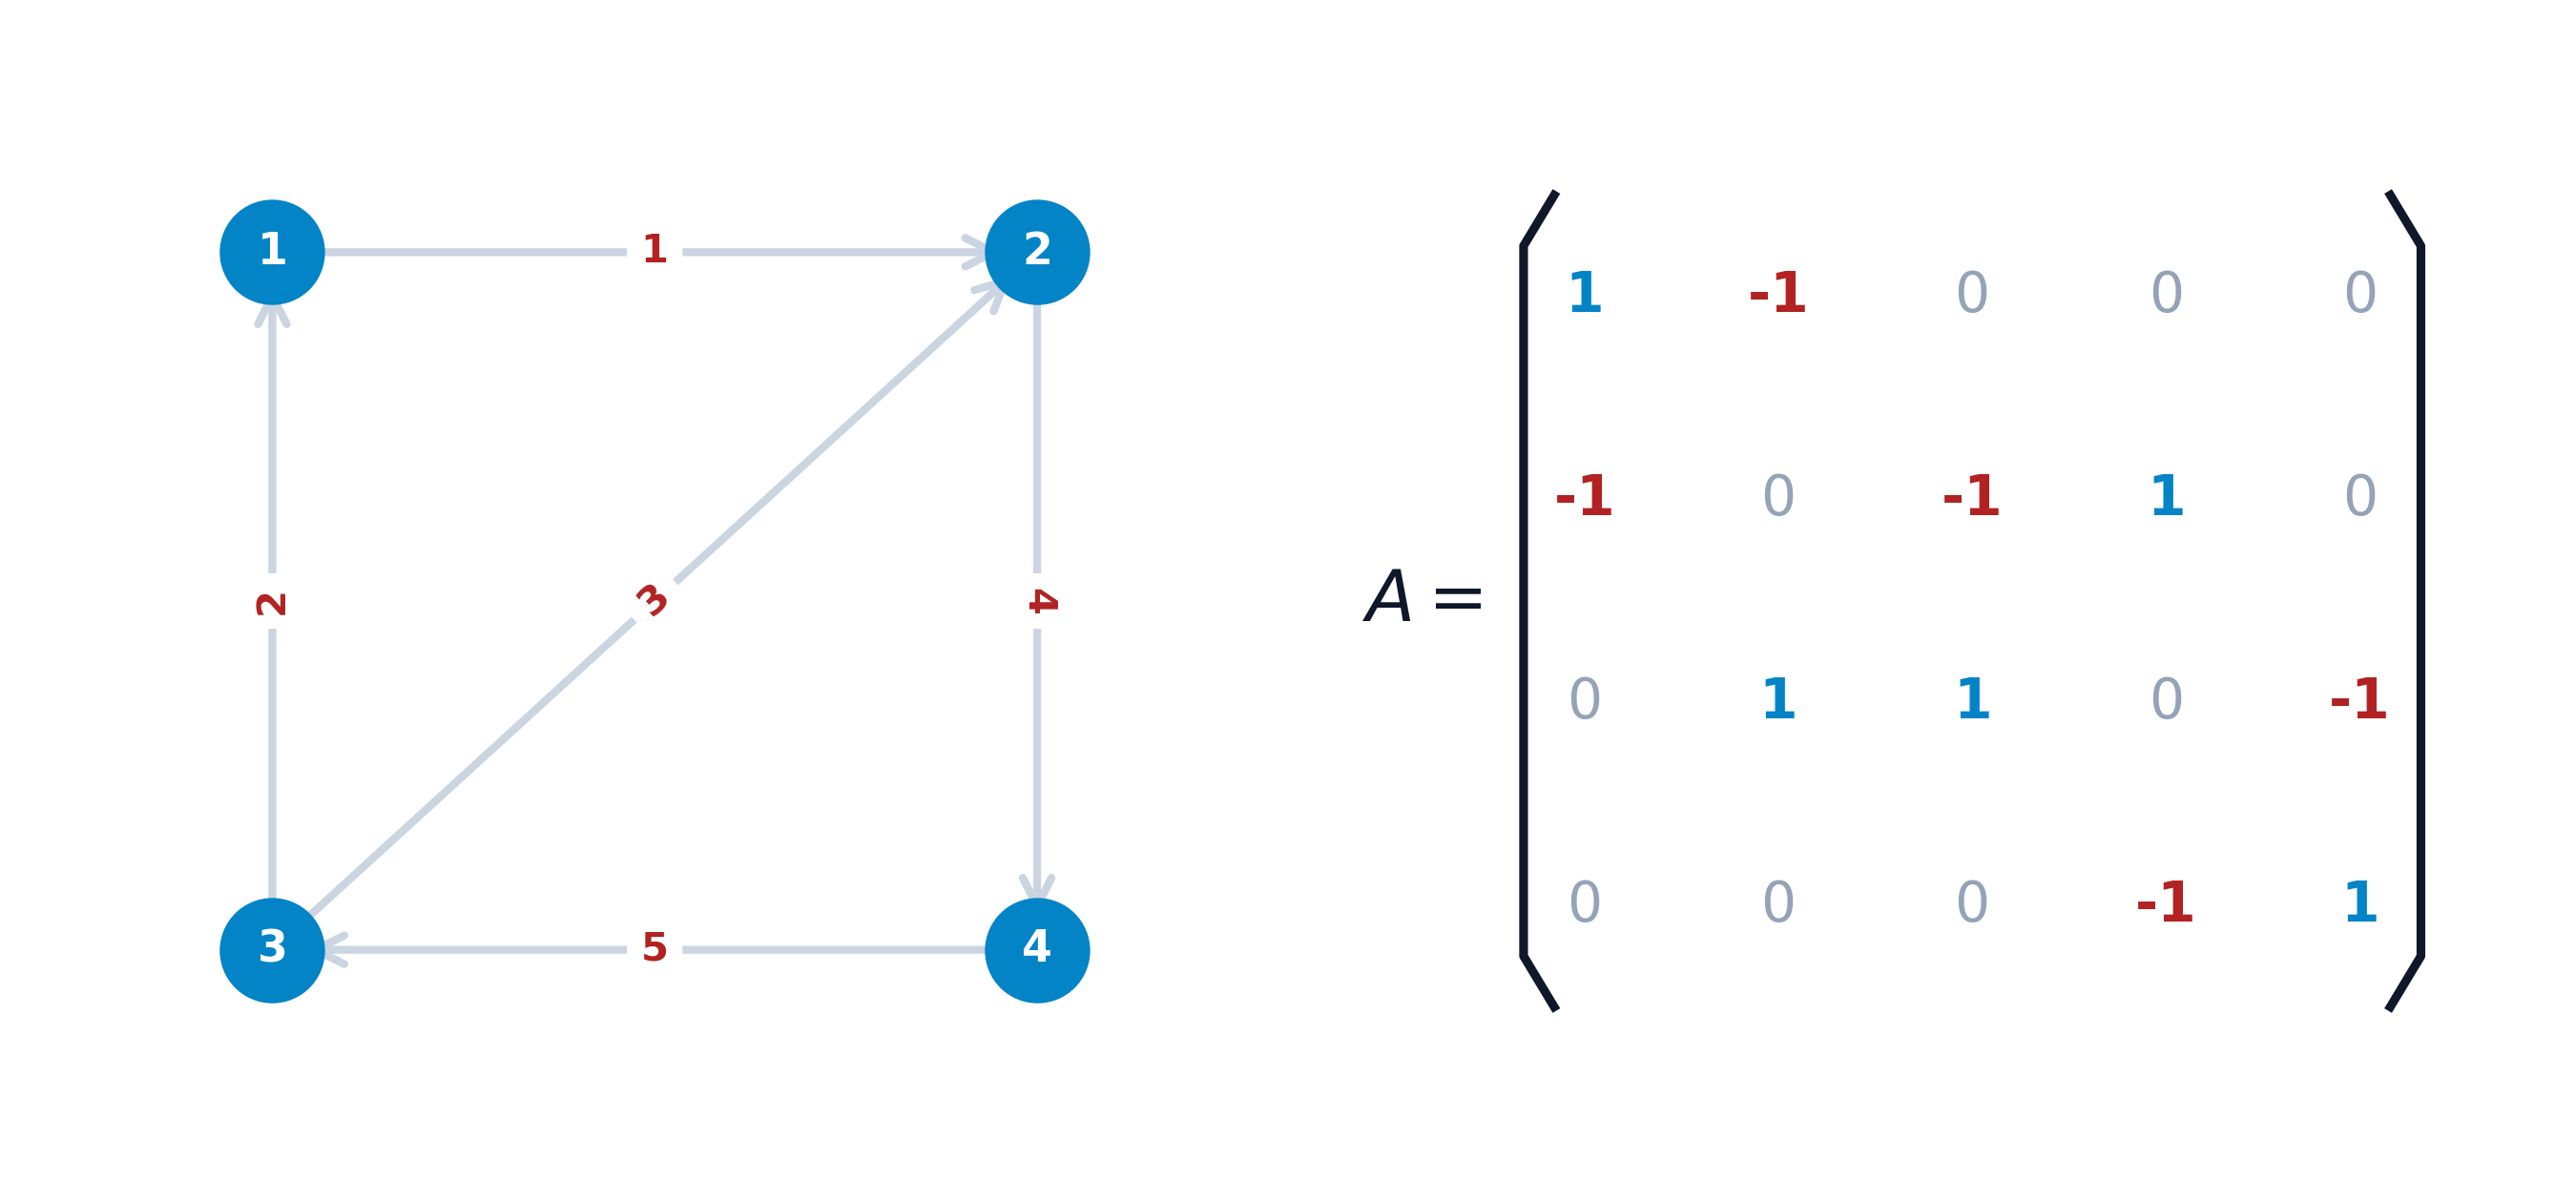
\includegraphics[width=0.9\linewidth,height=\textheight,keepaspectratio]{../images/matriz_incidencia_digrafo.png}
\end{center}
\end{column}
\end{columns}

\begin{itemize}
\tightlist
\item
  \textbf{Propiedad de Total Unimodularidad (TUM)}: Todo subdeterminante
  es \(0, \pm 1\), garantizando soluciones enteras en flujos.
\end{itemize}
\end{frame}

\begin{frame}{Matriz de adyacencia (Grafo no dirigido)}
\phantomsection\label{matriz-de-adyacencia-grafo-no-dirigido}
\begin{columns}[T]
\begin{column}{0.58\linewidth}
\begin{tcolorbox}[enhanced jigsaw, toptitle=1mm, opacityback=0, opacitybacktitle=0.6, colback=white, arc=.35mm, bottomrule=.15mm, titlerule=0mm, coltitle=black, breakable, bottomtitle=1mm, left=2mm, title=\textcolor{quarto-callout-note-color}{\faInfo}\hspace{0.5em}{Definición: Matriz de adyacencia no dirigida}, colbacktitle=quarto-callout-note-color!10!white, rightrule=.15mm, toprule=.15mm, colframe=quarto-callout-note-color-frame, leftrule=.75mm]

Dado un grafo simple no dirigido \(G = (V, E)\), la \textbf{matriz de
adyacencia} \(B \in \mathbb{R}^{n \times n}\) se define como: \[
\small
b_{ij} = \begin{cases} 
1 & \text{si } \{i, j\} \in E \\
0 & \text{en otro caso}
\end{cases}
\]

\end{tcolorbox}
\end{column}

\begin{column}{0.42\linewidth}
\begin{center}
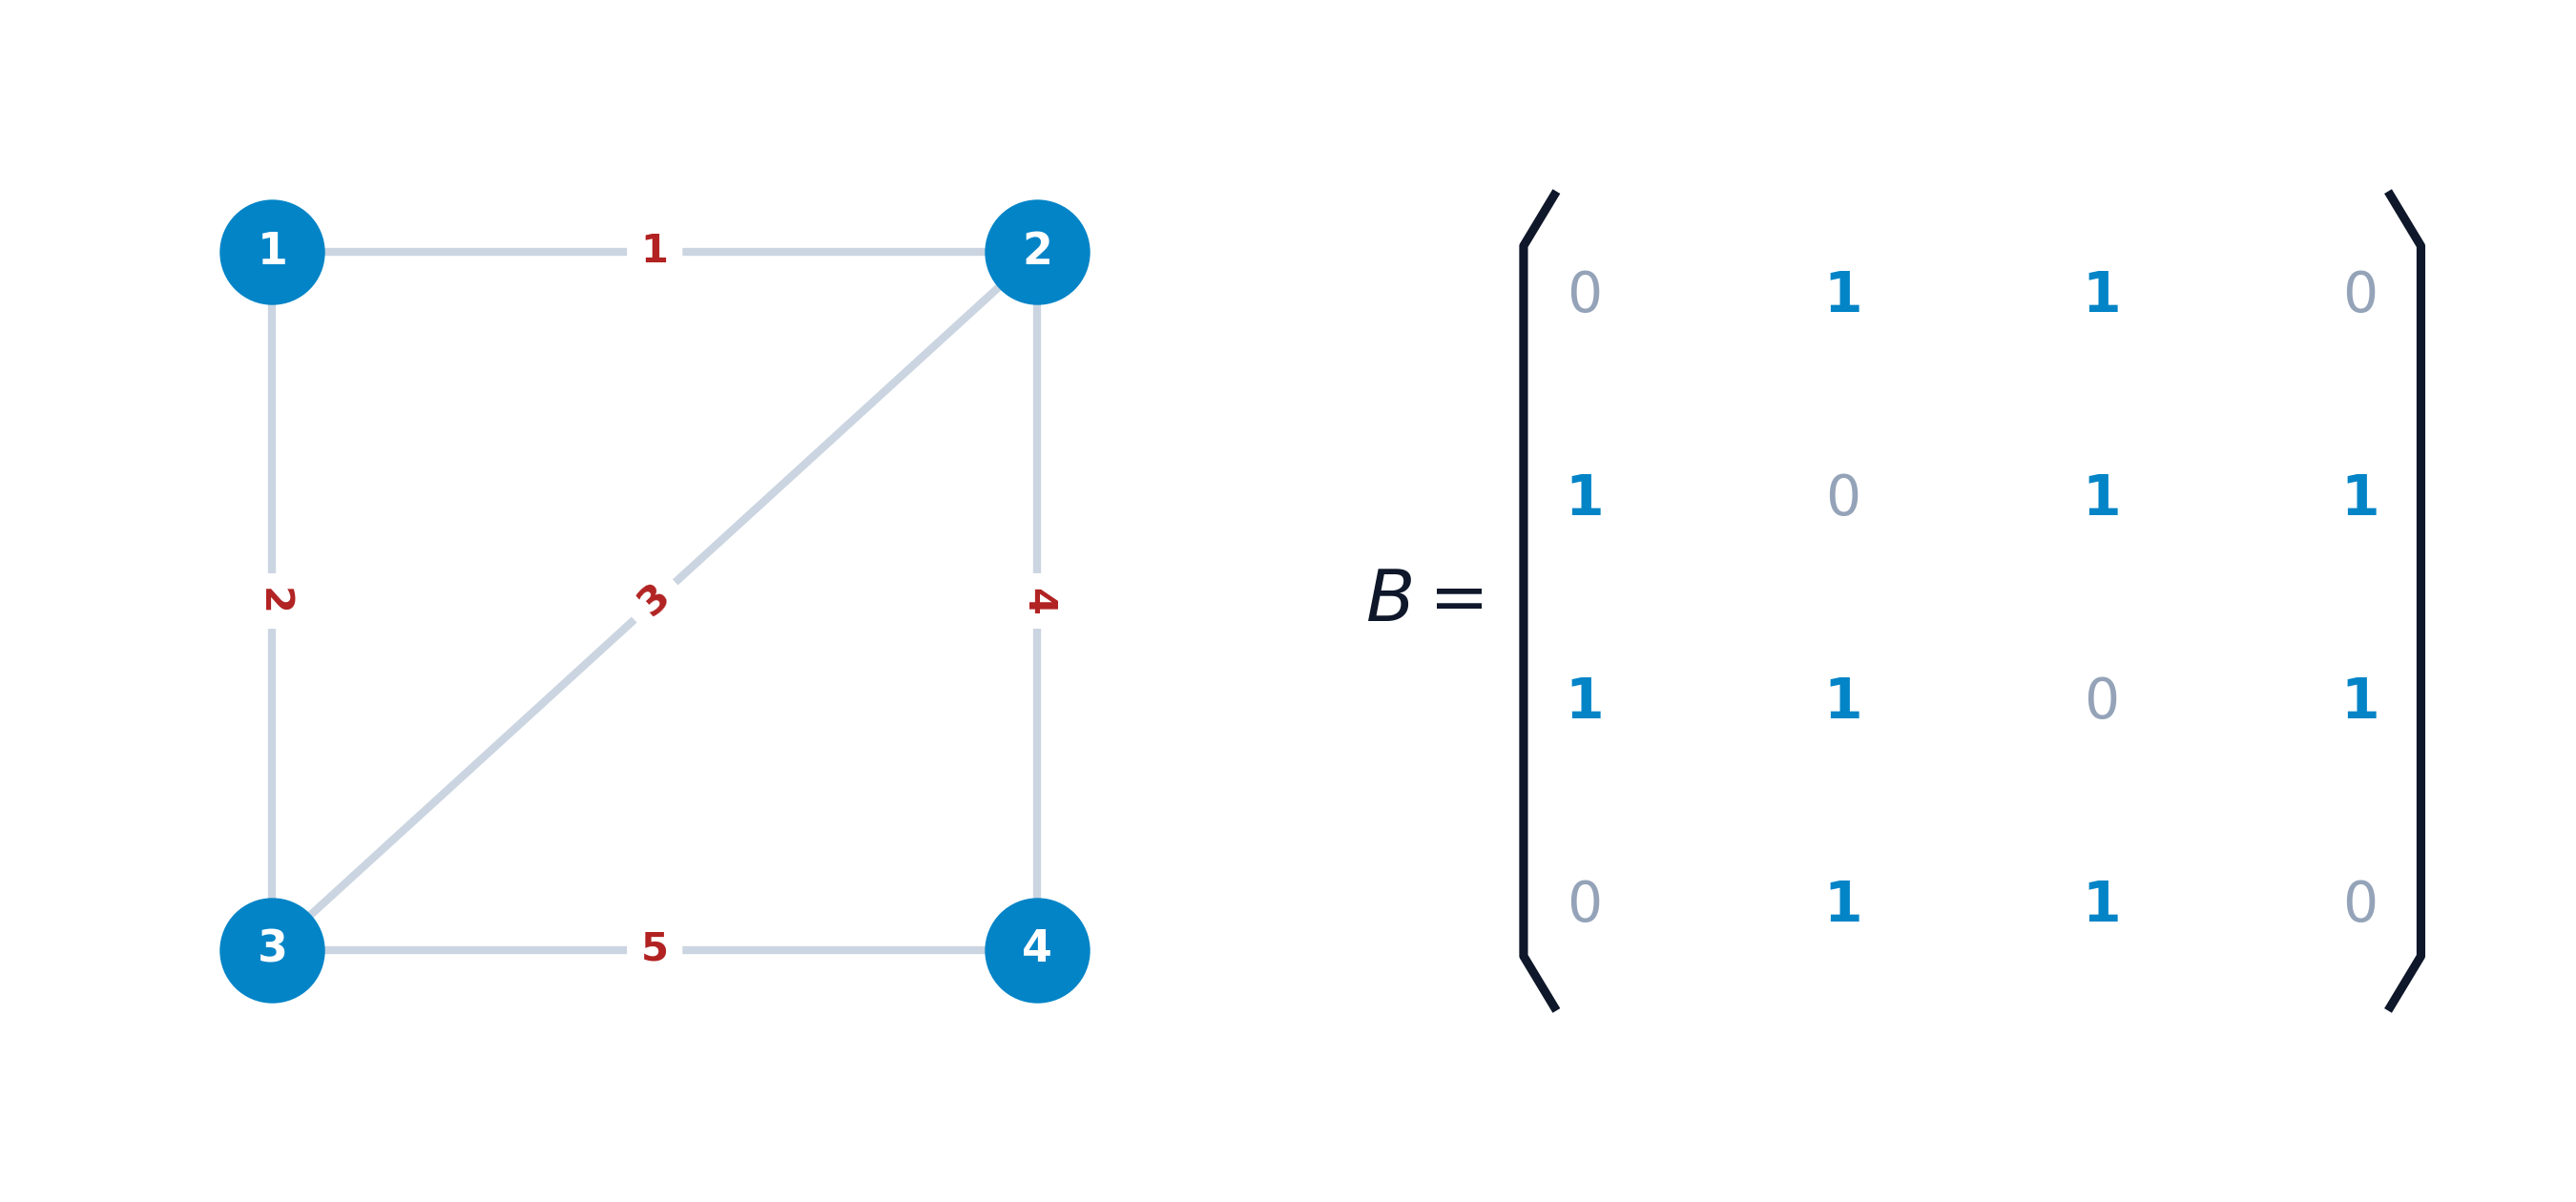
\includegraphics[width=0.9\linewidth,height=\textheight,keepaspectratio]{../images/matriz_adyacencia_grafo.png}
\end{center}
\end{column}
\end{columns}

\begin{itemize}
\tightlist
\item
  \textbf{Matriz simétrica}: \(B = B^T\) con ceros en la diagonal
  (\(b_{ii} = 0\)).
\end{itemize}
\end{frame}

\begin{frame}{Matriz de adyacencia (Digrafo)}
\phantomsection\label{matriz-de-adyacencia-digrafo}
\begin{columns}[T]
\begin{column}{0.58\linewidth}
\begin{tcolorbox}[enhanced jigsaw, toptitle=1mm, opacityback=0, opacitybacktitle=0.6, colback=white, arc=.35mm, bottomrule=.15mm, titlerule=0mm, coltitle=black, breakable, bottomtitle=1mm, left=2mm, title=\textcolor{quarto-callout-note-color}{\faInfo}\hspace{0.5em}{Definición: Matriz de adyacencia orientada}, colbacktitle=quarto-callout-note-color!10!white, rightrule=.15mm, toprule=.15mm, colframe=quarto-callout-note-color-frame, leftrule=.75mm]

Dado un digrafo \(G = (V, U)\), la matriz
\(B \in \mathbb{R}^{n \times n}\) es asimétrica: \[
\small
b_{ik} = \begin{cases} 
1 & \text{si } (i, k) \in U \\
0 & \text{en otro caso}
\end{cases}
\]

\end{tcolorbox}
\end{column}

\begin{column}{0.42\linewidth}
\begin{center}
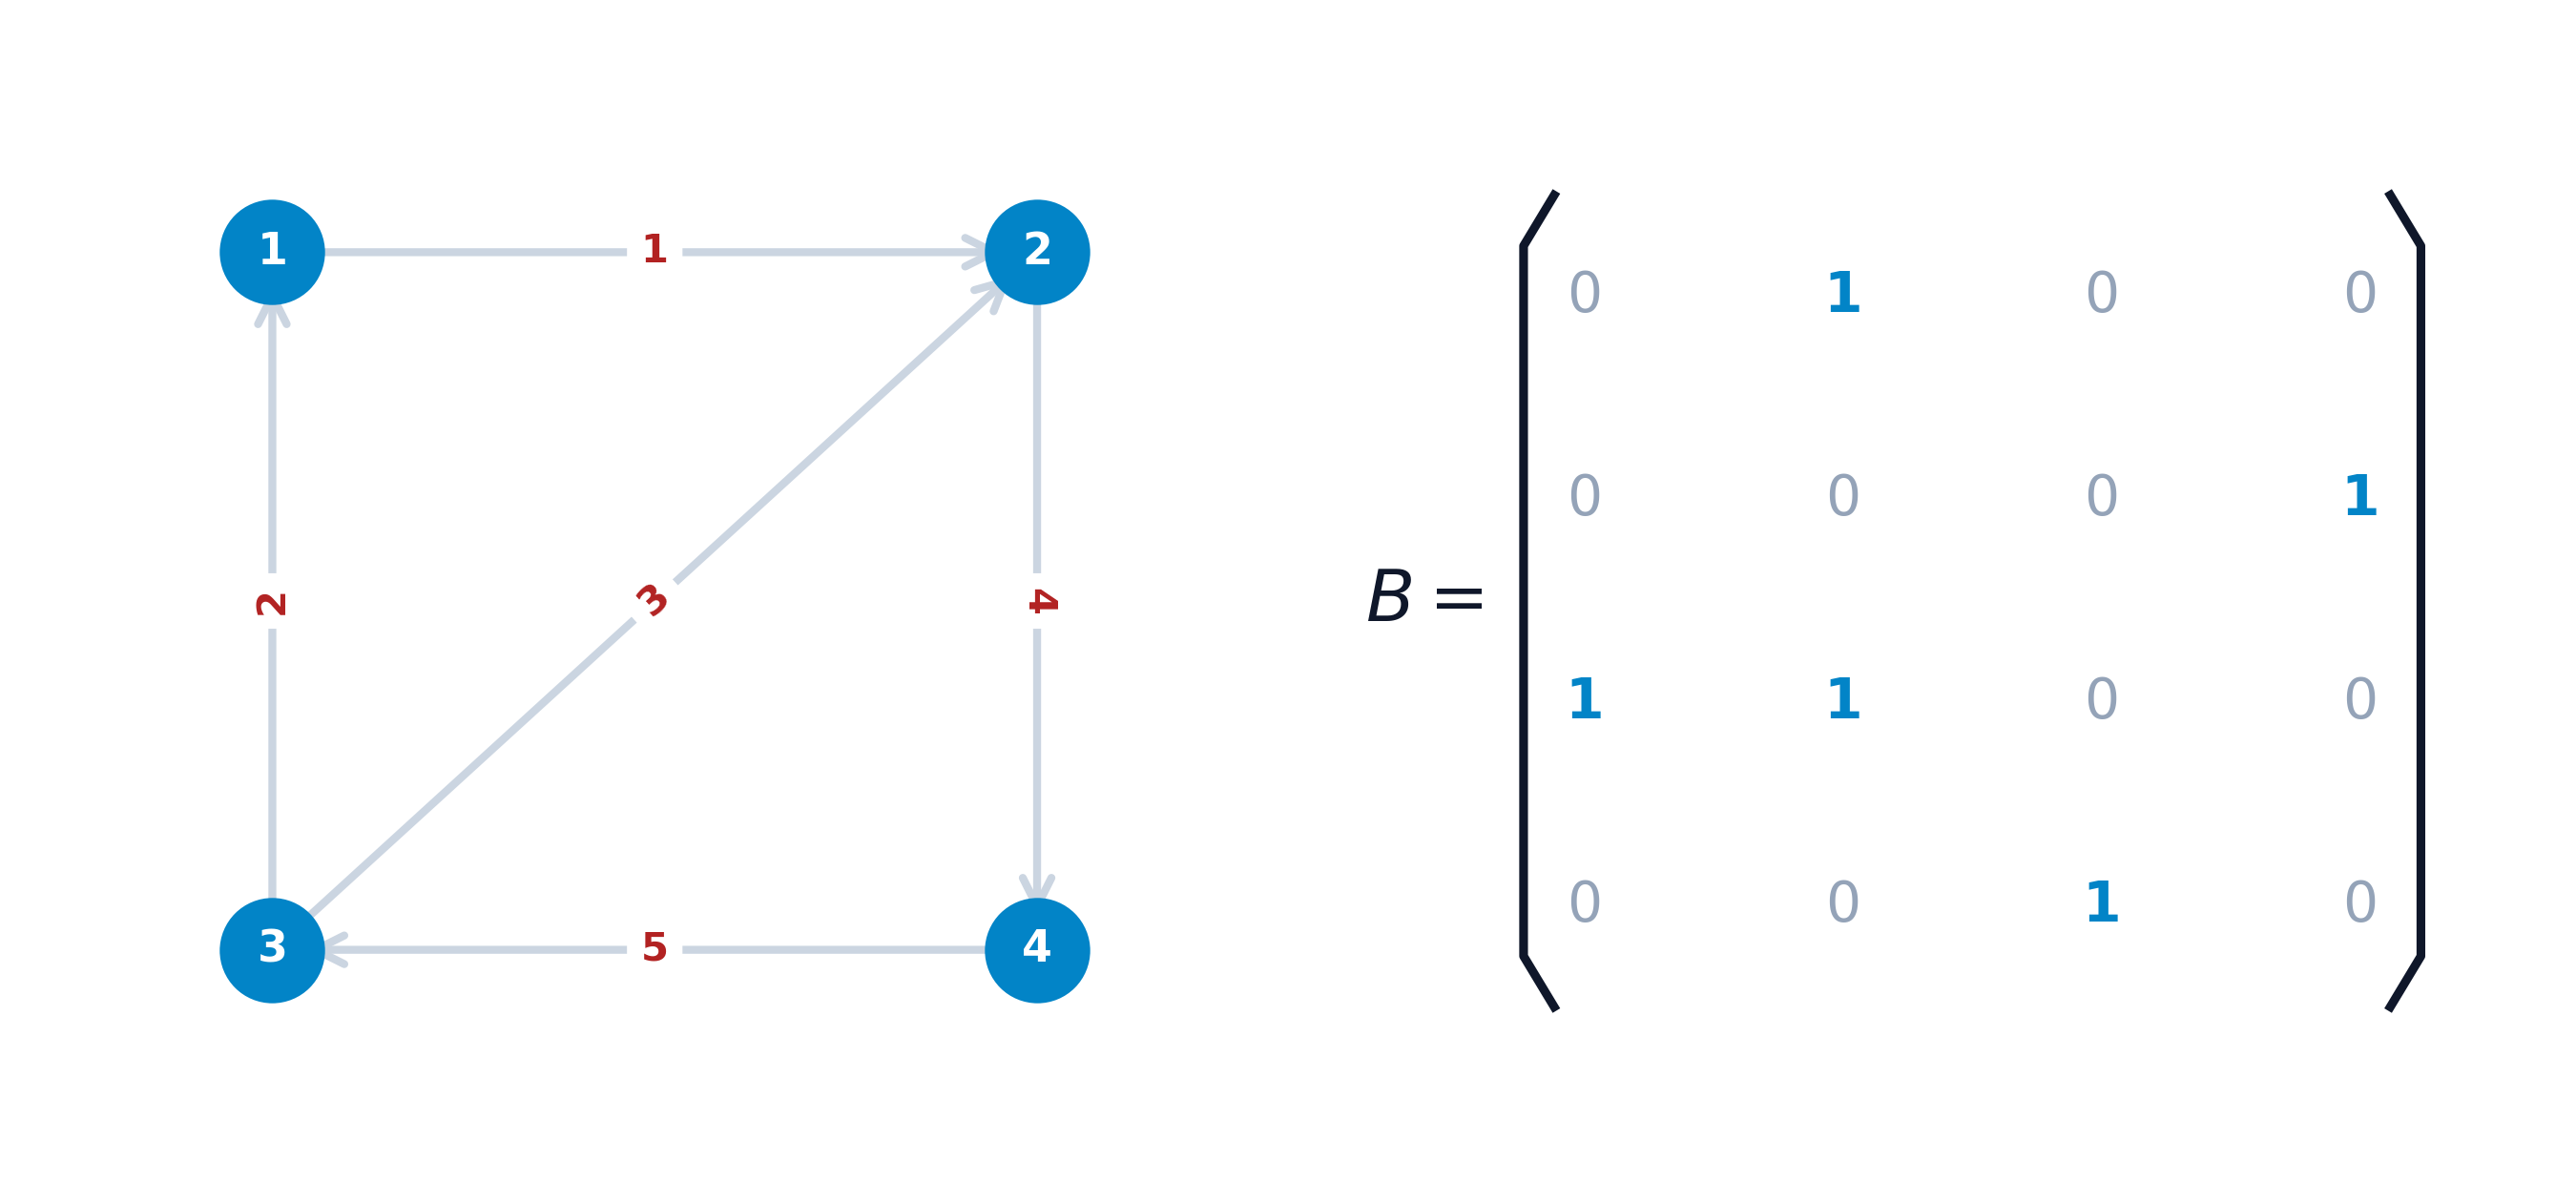
\includegraphics[width=0.9\linewidth,height=\textheight,keepaspectratio]{../images/matriz_adyacencia_digrafo.png}
\end{center}
\end{column}
\end{columns}

\begin{itemize}
\tightlist
\item
  \textbf{Conteo de caminos}: El elemento \((B^p)_{ik}\) de la potencia
  \(B^p\) indica el número exacto de caminos de longitud \(p\) entre los
  nodos \(i\) y \(k\).
\end{itemize}
\end{frame}

\begin{frame}{Motivación: Redes dispersas y almacenamiento}
\phantomsection\label{motivaciuxf3n-redes-dispersas-y-almacenamiento}
\begin{itemize}
\item
  \textbf{Inconveniente de matrices densas}: En redes dispersas (donde
  el número de arcos es mucho menor que el cuadrado de nodos,
  \(m \ll n^2\)), las matrices de adyacencia o incidencia almacenan más
  del \(99\%\) de entradas nulas (ceros).
\item
  \textbf{Almacenamiento lineal eficiente}: Para optimizar el uso de
  memoria y la velocidad de cómputo, las matrices se sustituyen por dos
  vectores unidimensionales de dimensión reducida:

  \begin{itemize}
  \tightlist
  \item
    \textbf{Vector \(\beta\)} (dimensión \(m\)): Almacena los nodos de
    destino.
  \item
    \textbf{Vector \(\alpha\)} (dimensión \(n+1\)): Almacena los
    punteros de inicio.
  \end{itemize}
\end{itemize}
\end{frame}

\begin{frame}{Esquema de punteros (\(\alpha, \beta\)) en digrafos}
\phantomsection\label{esquema-de-punteros-alpha-beta-en-digrafos}
\begin{columns}[T]
\begin{column}{0.5\linewidth}
\begin{itemize}
\item
  \textbf{Vector \(\beta\)} (dimensión \(m\)): Contiene los nodos de
  destino \(j\) de todos los arcos \((i, j) \in U\), agrupados en orden
  lexicográfico según el nodo origen \(i\).
\item
  \textbf{Vector \(\alpha\)} (dimensión \(n+1\)): Punteros que indican
  la posición en \(\beta\) donde comienzan los arcos salientes de cada
  nodo \(i\).

  \begin{itemize}
  \tightlist
  \item
    \textbf{Condición de cierre}: \(\alpha(n+1) = m + 1\).
  \end{itemize}
\end{itemize}
\end{column}

\begin{column}{0.5\linewidth}
\pandocbounded{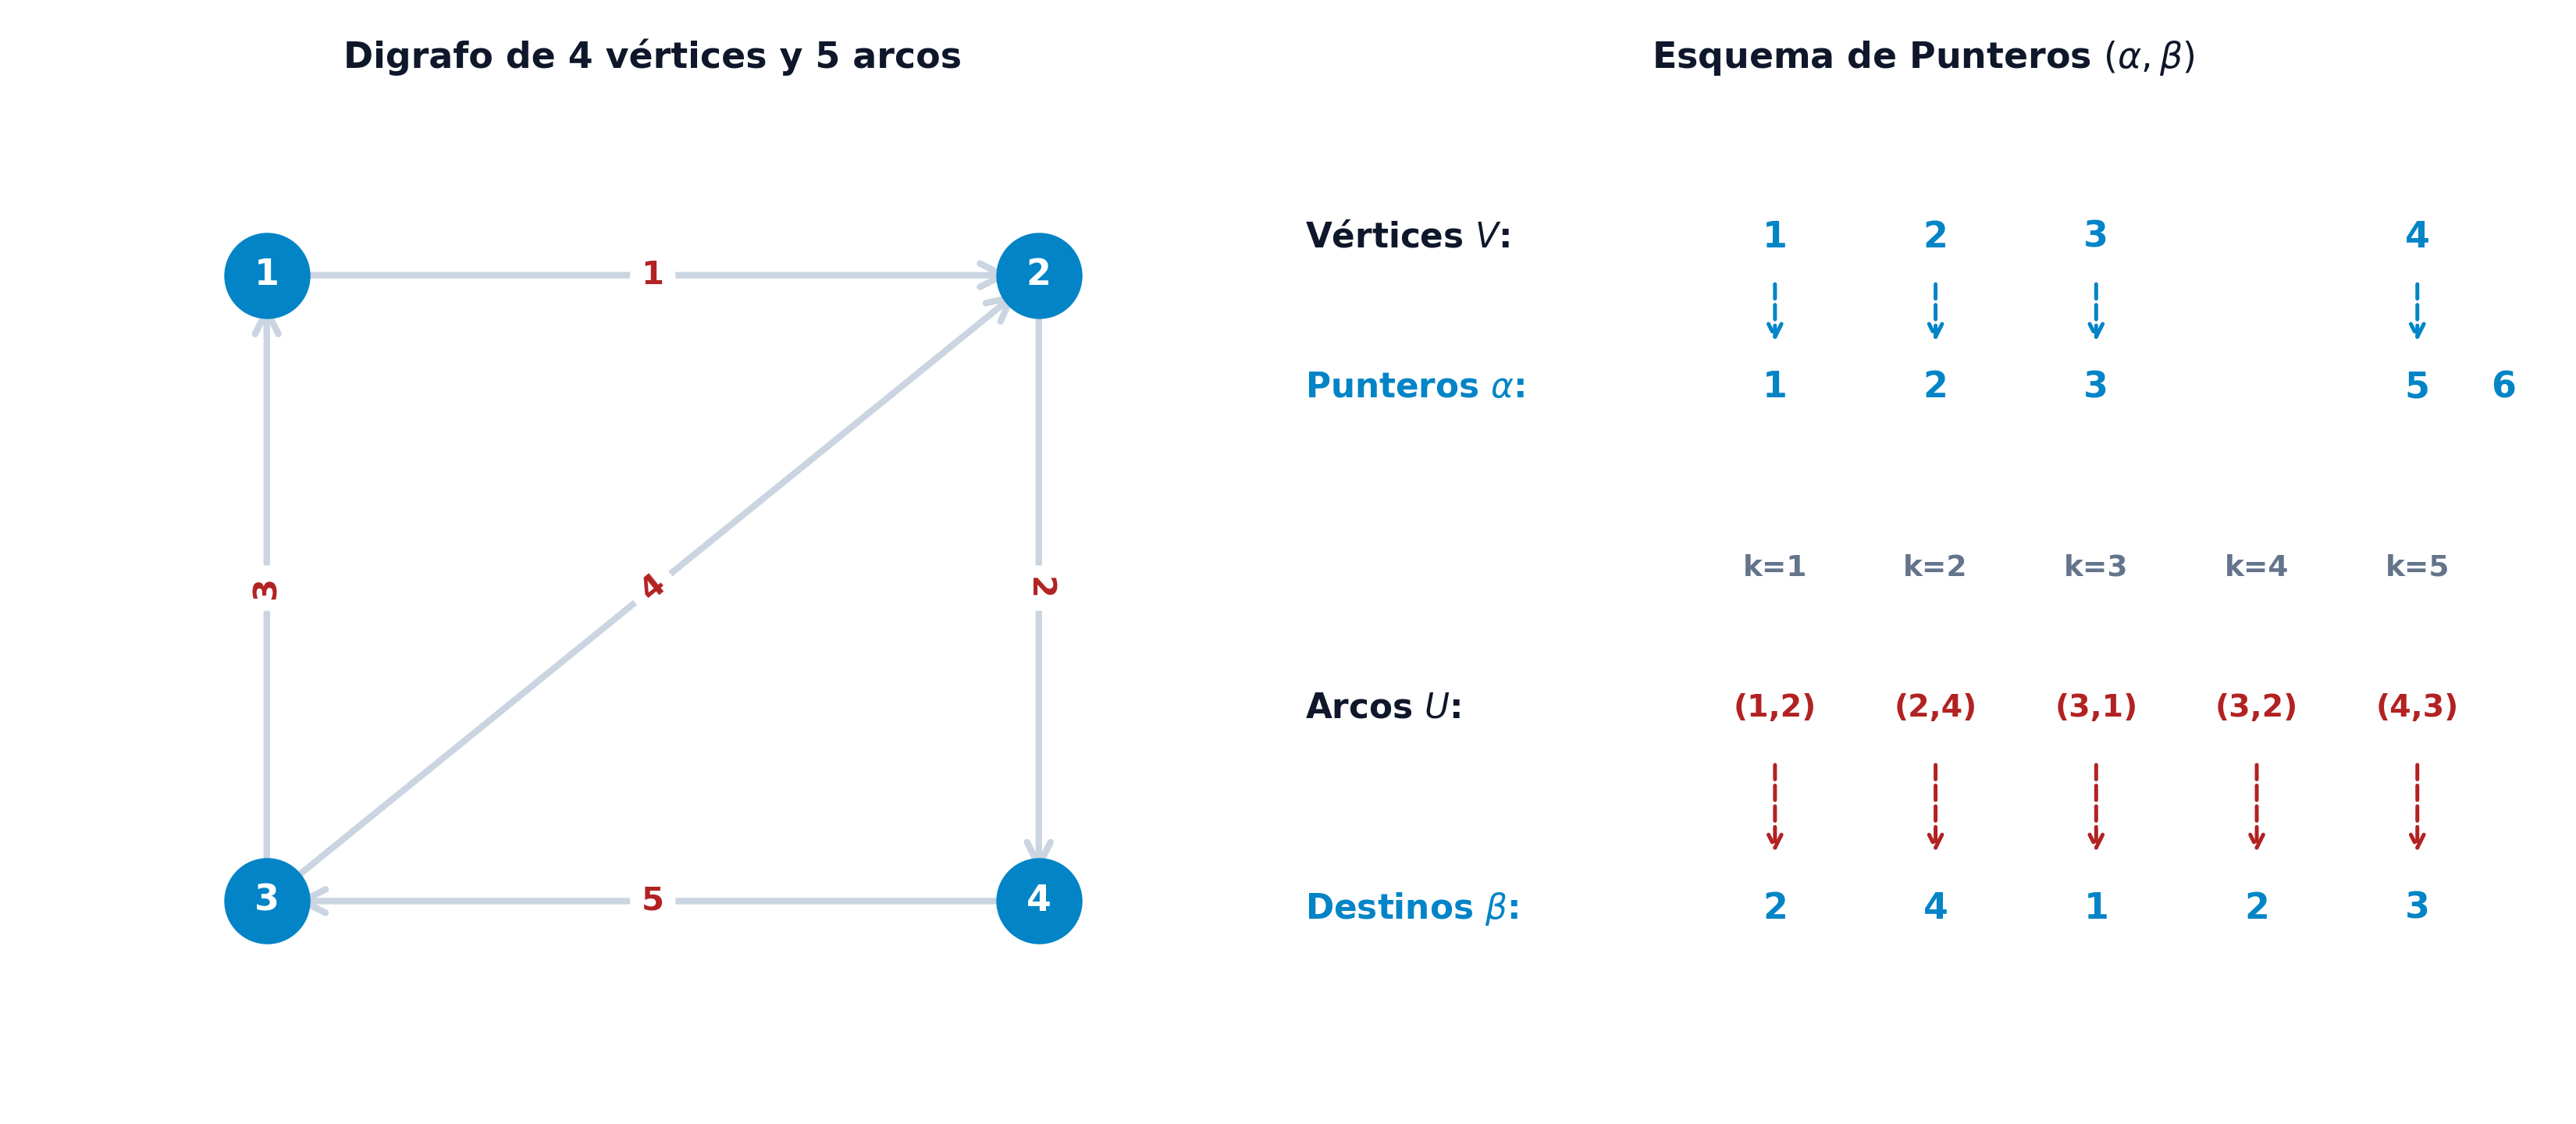
\includegraphics[keepaspectratio]{../images/representacion_vectorial_digrafo.png}}
\end{column}
\end{columns}
\end{frame}

\begin{frame}{Ejemplo: Evaluación de vectores (\(\alpha, \beta\)) en
redes}
\phantomsection\label{ejemplo-evaluaciuxf3n-de-vectores-alpha-beta-en-redes}
\begin{columns}[T]
\begin{column}{0.5\linewidth}
\begin{itemize}
\item
  \textbf{Recurrencia regresiva para \(\alpha\)}: \[
  \alpha(k) = \alpha(k+1) - d^+(k)
  \] con la condición inicial \(\alpha(n+1) = m + 1\).
\item
  \textbf{Evaluación en la red (\(n=6, m=10\))}:

  \begin{itemize}
  \tightlist
  \item
    Condición inicial: \(\alpha(7) = 10 + 1 = 11\).
  \item
    Vector de destinos \(\beta \in \mathbb{R}^{10}\).
  \item
    Vector de punteros resultante: \[\alpha = (1, 4, 5, 7, 10, 11, 11)\]
  \end{itemize}
\end{itemize}
\end{column}

\begin{column}{0.5\linewidth}
\pandocbounded{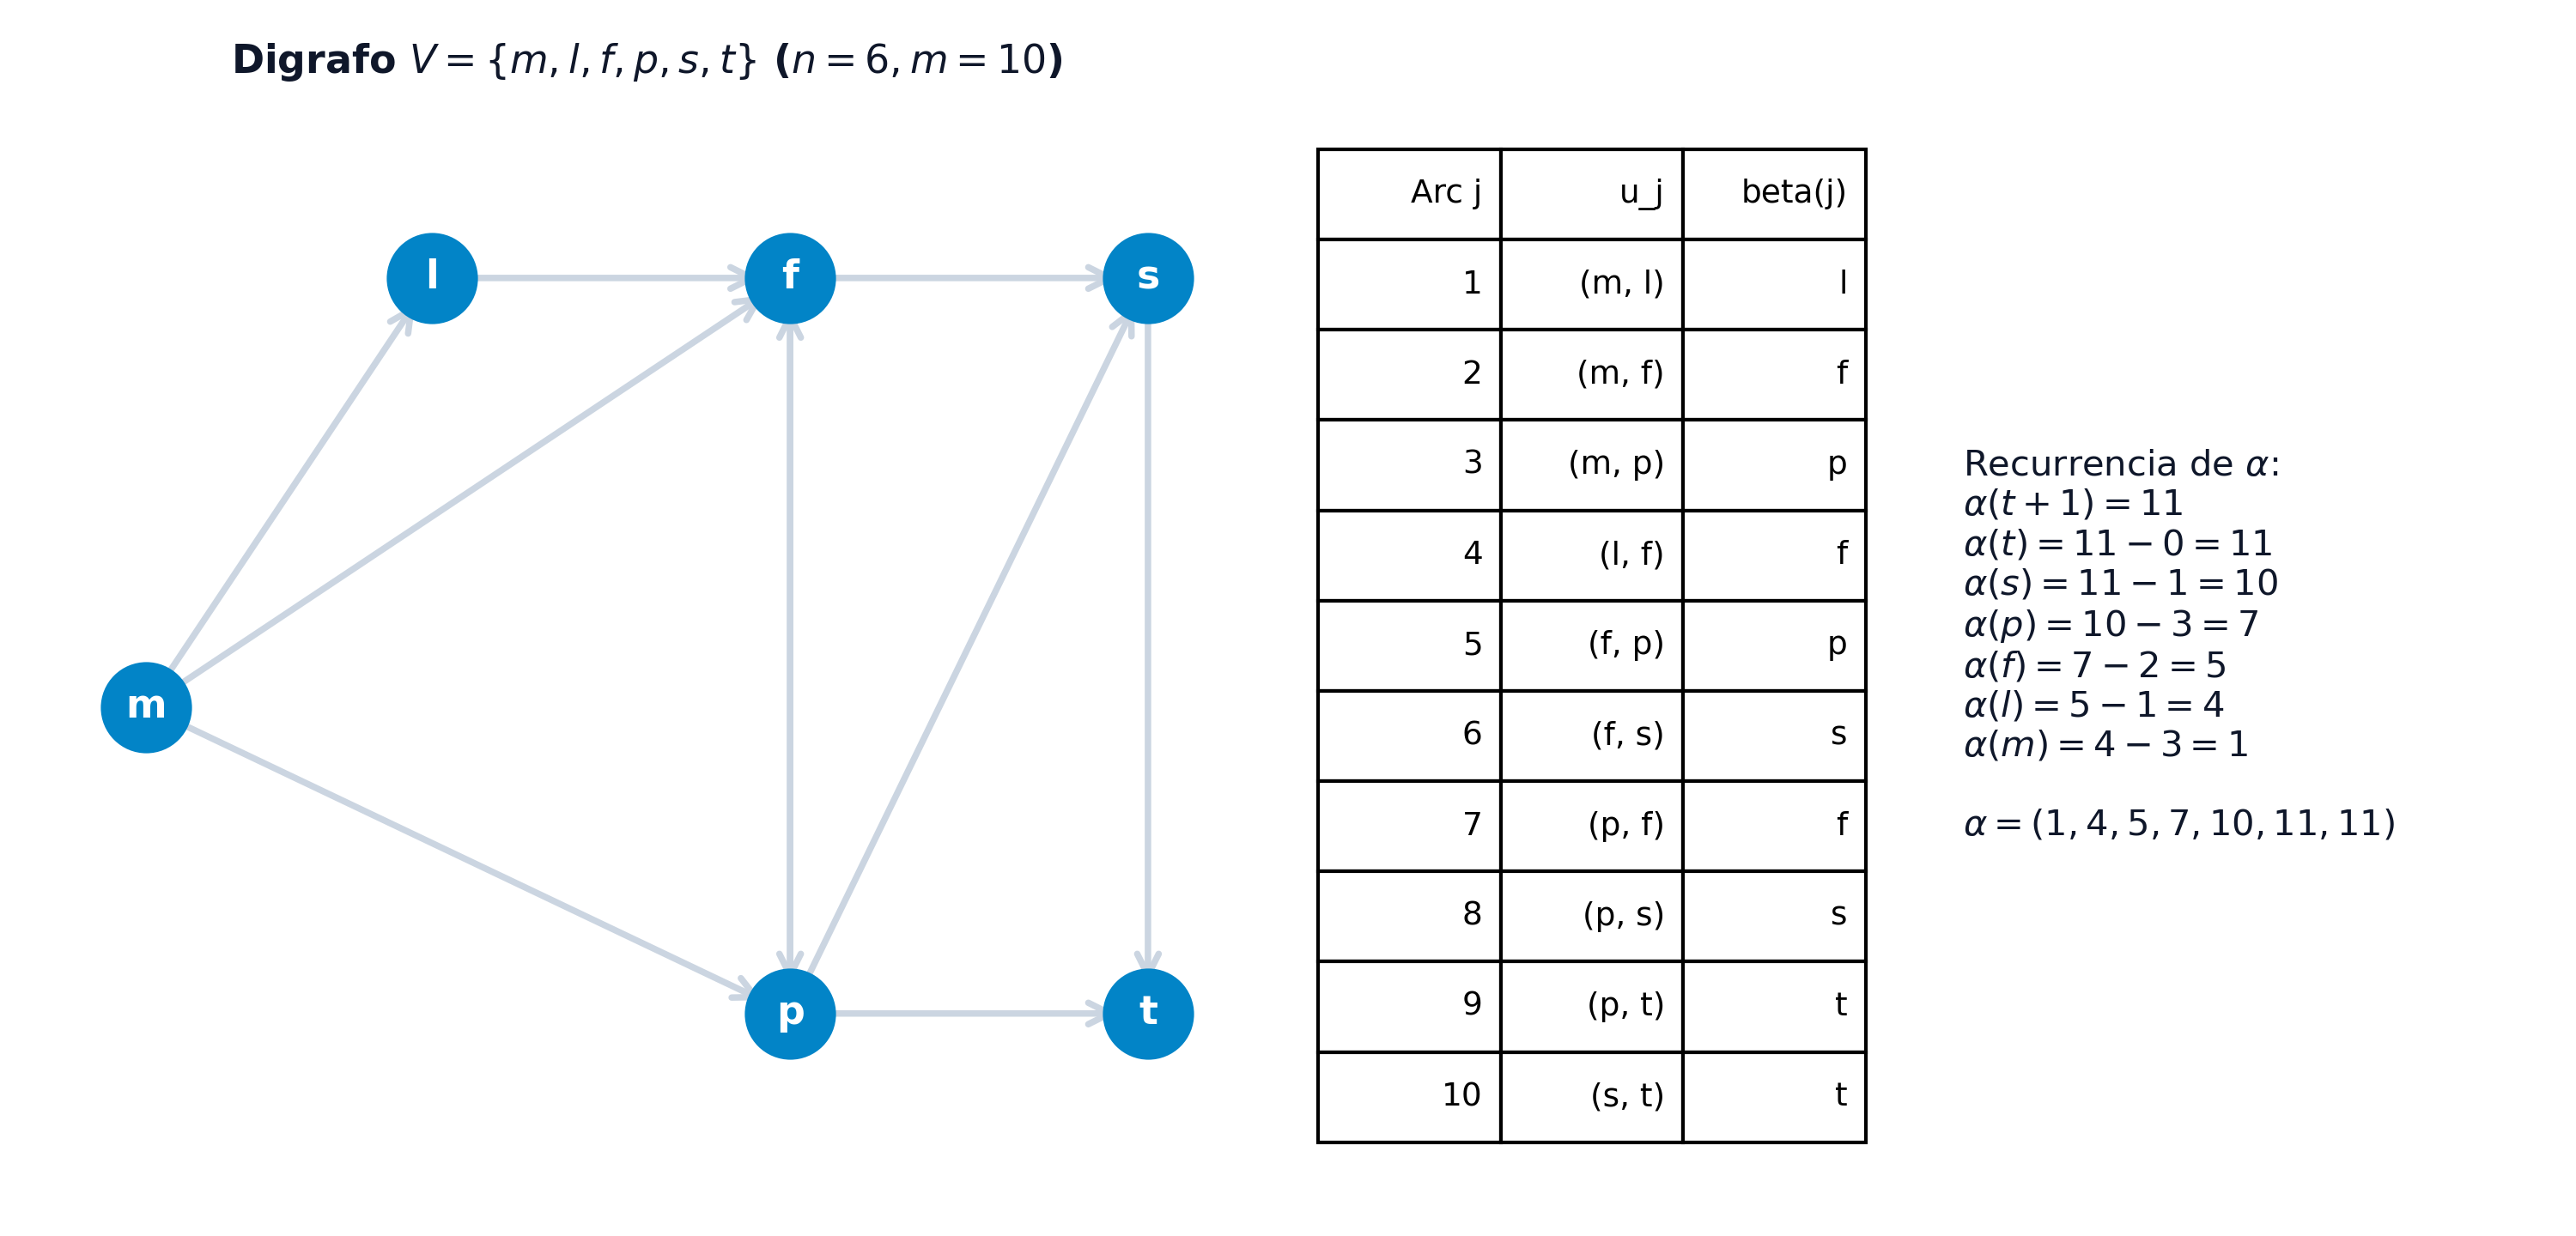
\includegraphics[keepaspectratio]{../images/representacion_vectorial_ejemplo_complejo.png}}
\end{column}
\end{columns}
\end{frame}

\begin{frame}{Representación vectorial en grafos no dirigidos}
\phantomsection\label{representaciuxf3n-vectorial-en-grafos-no-dirigidos}
\begin{columns}[T]
\begin{column}{0.5\linewidth}
\begin{itemize}
\item
  \textbf{Descomposición bidireccional}: En grafos no dirigidos
  \(G = (V, E)\), cada arista \(\{i, j\}\) se descompone en dos arcos
  orientados opuestos \((i, j)\) y \((j, i)\).
\item
  \textbf{Dimensiones de los vectores}:

  \begin{itemize}
  \tightlist
  \item
    \textbf{Vector \(\beta\)}: Duplica su dimensión a \(2m\) elementos
    para registrar ambas direcciones.
  \item
    \textbf{Vector \(\alpha\)}: Mantiene la dimensión \(n+1\) con
    \(\alpha(n+1) = 2m + 1\).
  \end{itemize}
\end{itemize}
\end{column}

\begin{column}{0.5\linewidth}
\pandocbounded{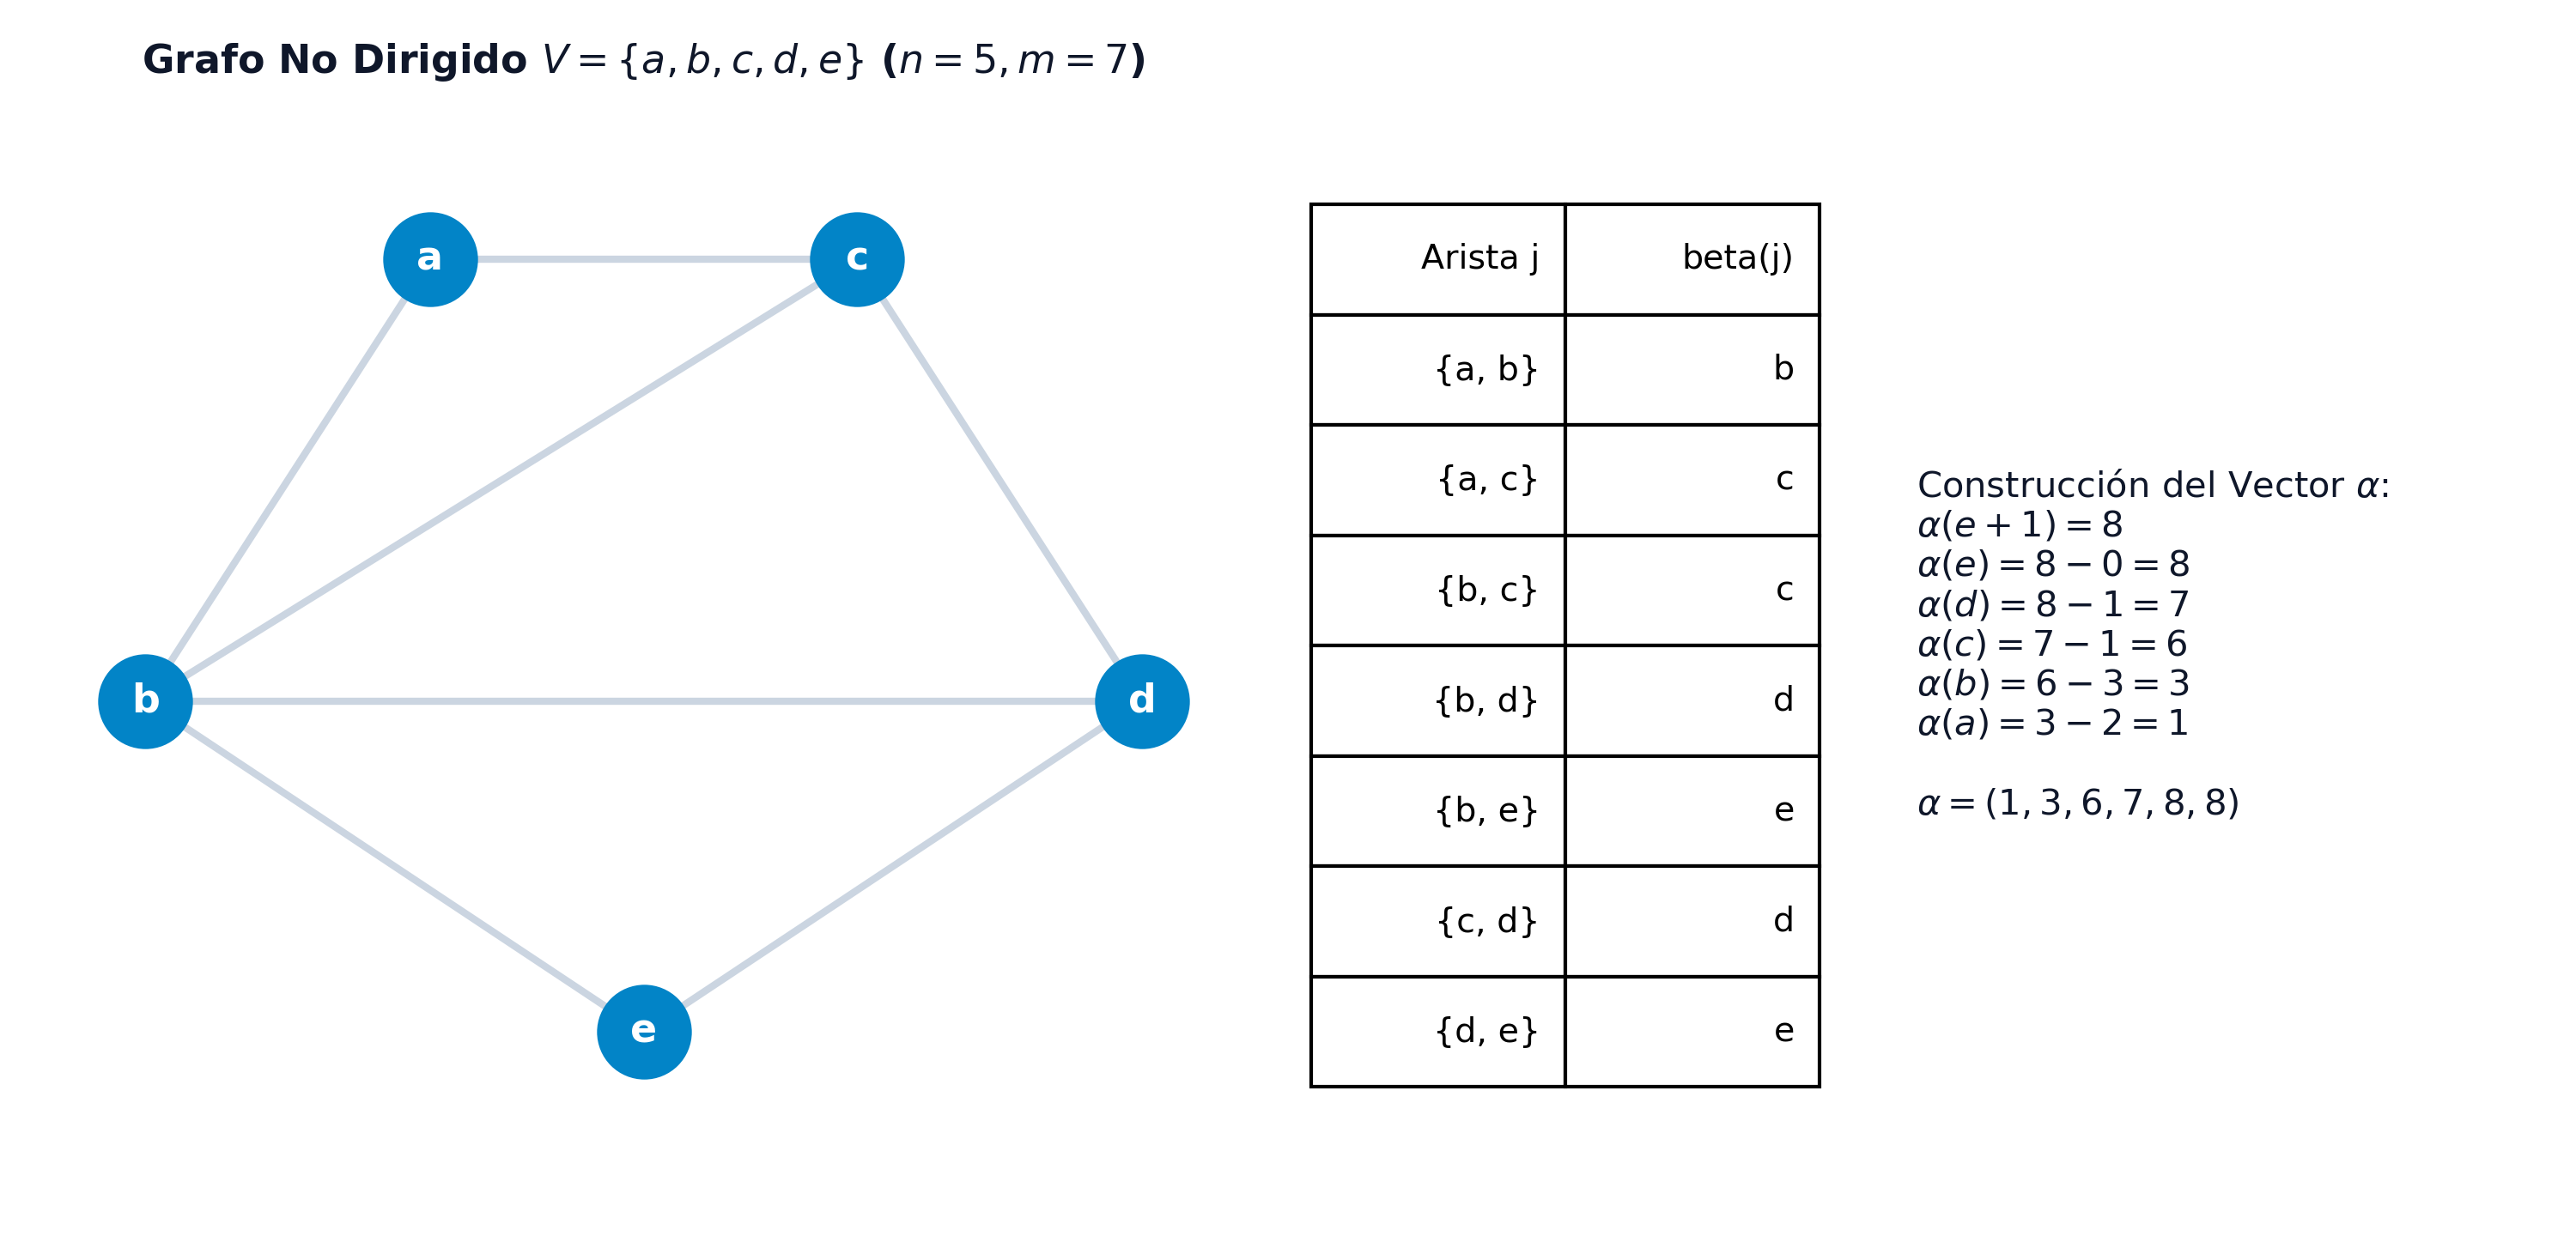
\includegraphics[keepaspectratio]{../images/representacion_vectorial_grafo_nodirigido.png}}
\end{column}
\end{columns}
\end{frame}

\begin{frame}{Listas de adyacencia en digrafos}
\phantomsection\label{listas-de-adyacencia-en-digrafos}
\begin{columns}[T]
\begin{column}{0.5\linewidth}
\begin{itemize}
\item
  \textbf{Estructura dinámica}: Arreglo de punteros \(\text{Adj}[i]\)
  donde cada nodo \(i\) encadena la lista de sus nodos sucesores
  \(\Gamma^+(i)\).
\item
  \textbf{Propiedades computacionales}:

  \begin{itemize}
  \tightlist
  \item
    \textbf{Memoria óptima}: Complejidad espacial \(O(n + m)\).
  \item
    \textbf{Eficiencia dinámica}: Permite insertar y eliminar arcos de
    forma dinámica con tiempo \(O(1)\).
  \end{itemize}
\end{itemize}
\end{column}

\begin{column}{0.5\linewidth}
\pandocbounded{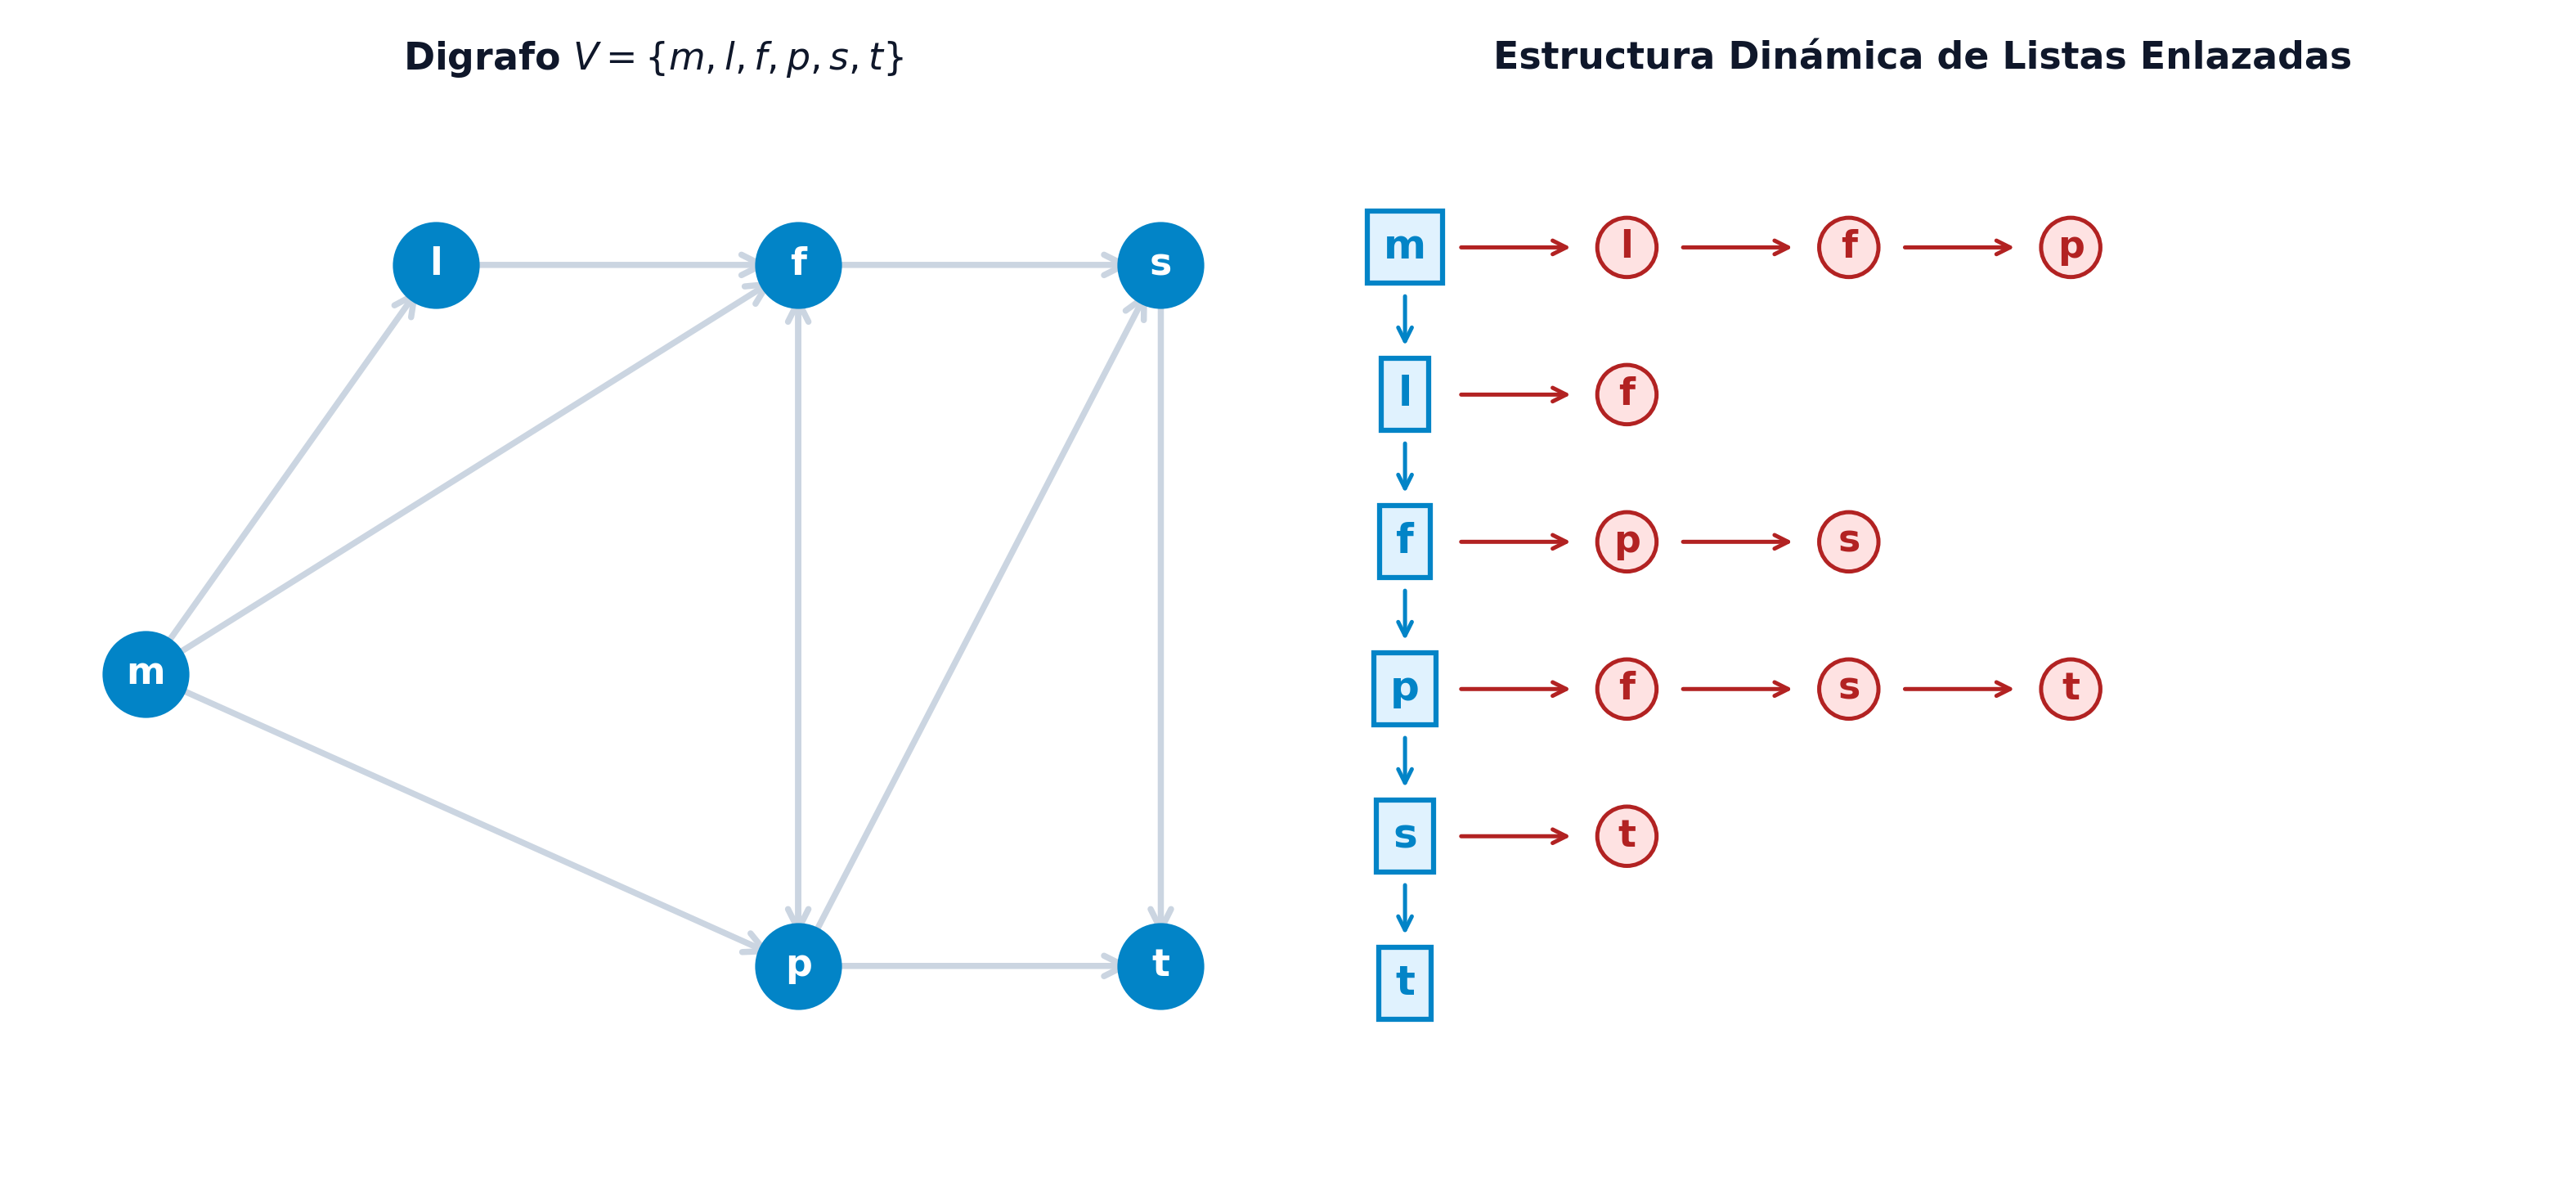
\includegraphics[keepaspectratio]{../images/lista_adyacencia_digrafo.png}}
\end{column}
\end{columns}
\end{frame}

\begin{frame}{Listas de adyacencia en grafos no dirigidos}
\phantomsection\label{listas-de-adyacencia-en-grafos-no-dirigidos}
\begin{columns}[T]
\begin{column}{0.5\linewidth}
\begin{itemize}
\tightlist
\item
  \textbf{Listas enlazadas recíprocas}: En grafos no dirigidos
  \(G = (V, E)\), cada arista no dirigida \(\{u, v\}\) genera dos
  entradas recíprocas en las estructuras enlazadas:

  \begin{itemize}
  \tightlist
  \item
    El nodo \(v\) se añade a la lista \(\text{Adj}[u]\).
  \item
    Simétricamente, el nodo \(u\) se incorpora a la lista
    \(\text{Adj}[v]\).
  \end{itemize}
\item
  \textbf{Ejemplo sobre \(V = \{a, b, c, d, e\}\)}: Representación en
  red de 5 vértices con conexiones simétricas bidireccionales.
\end{itemize}
\end{column}

\begin{column}{0.5\linewidth}
\pandocbounded{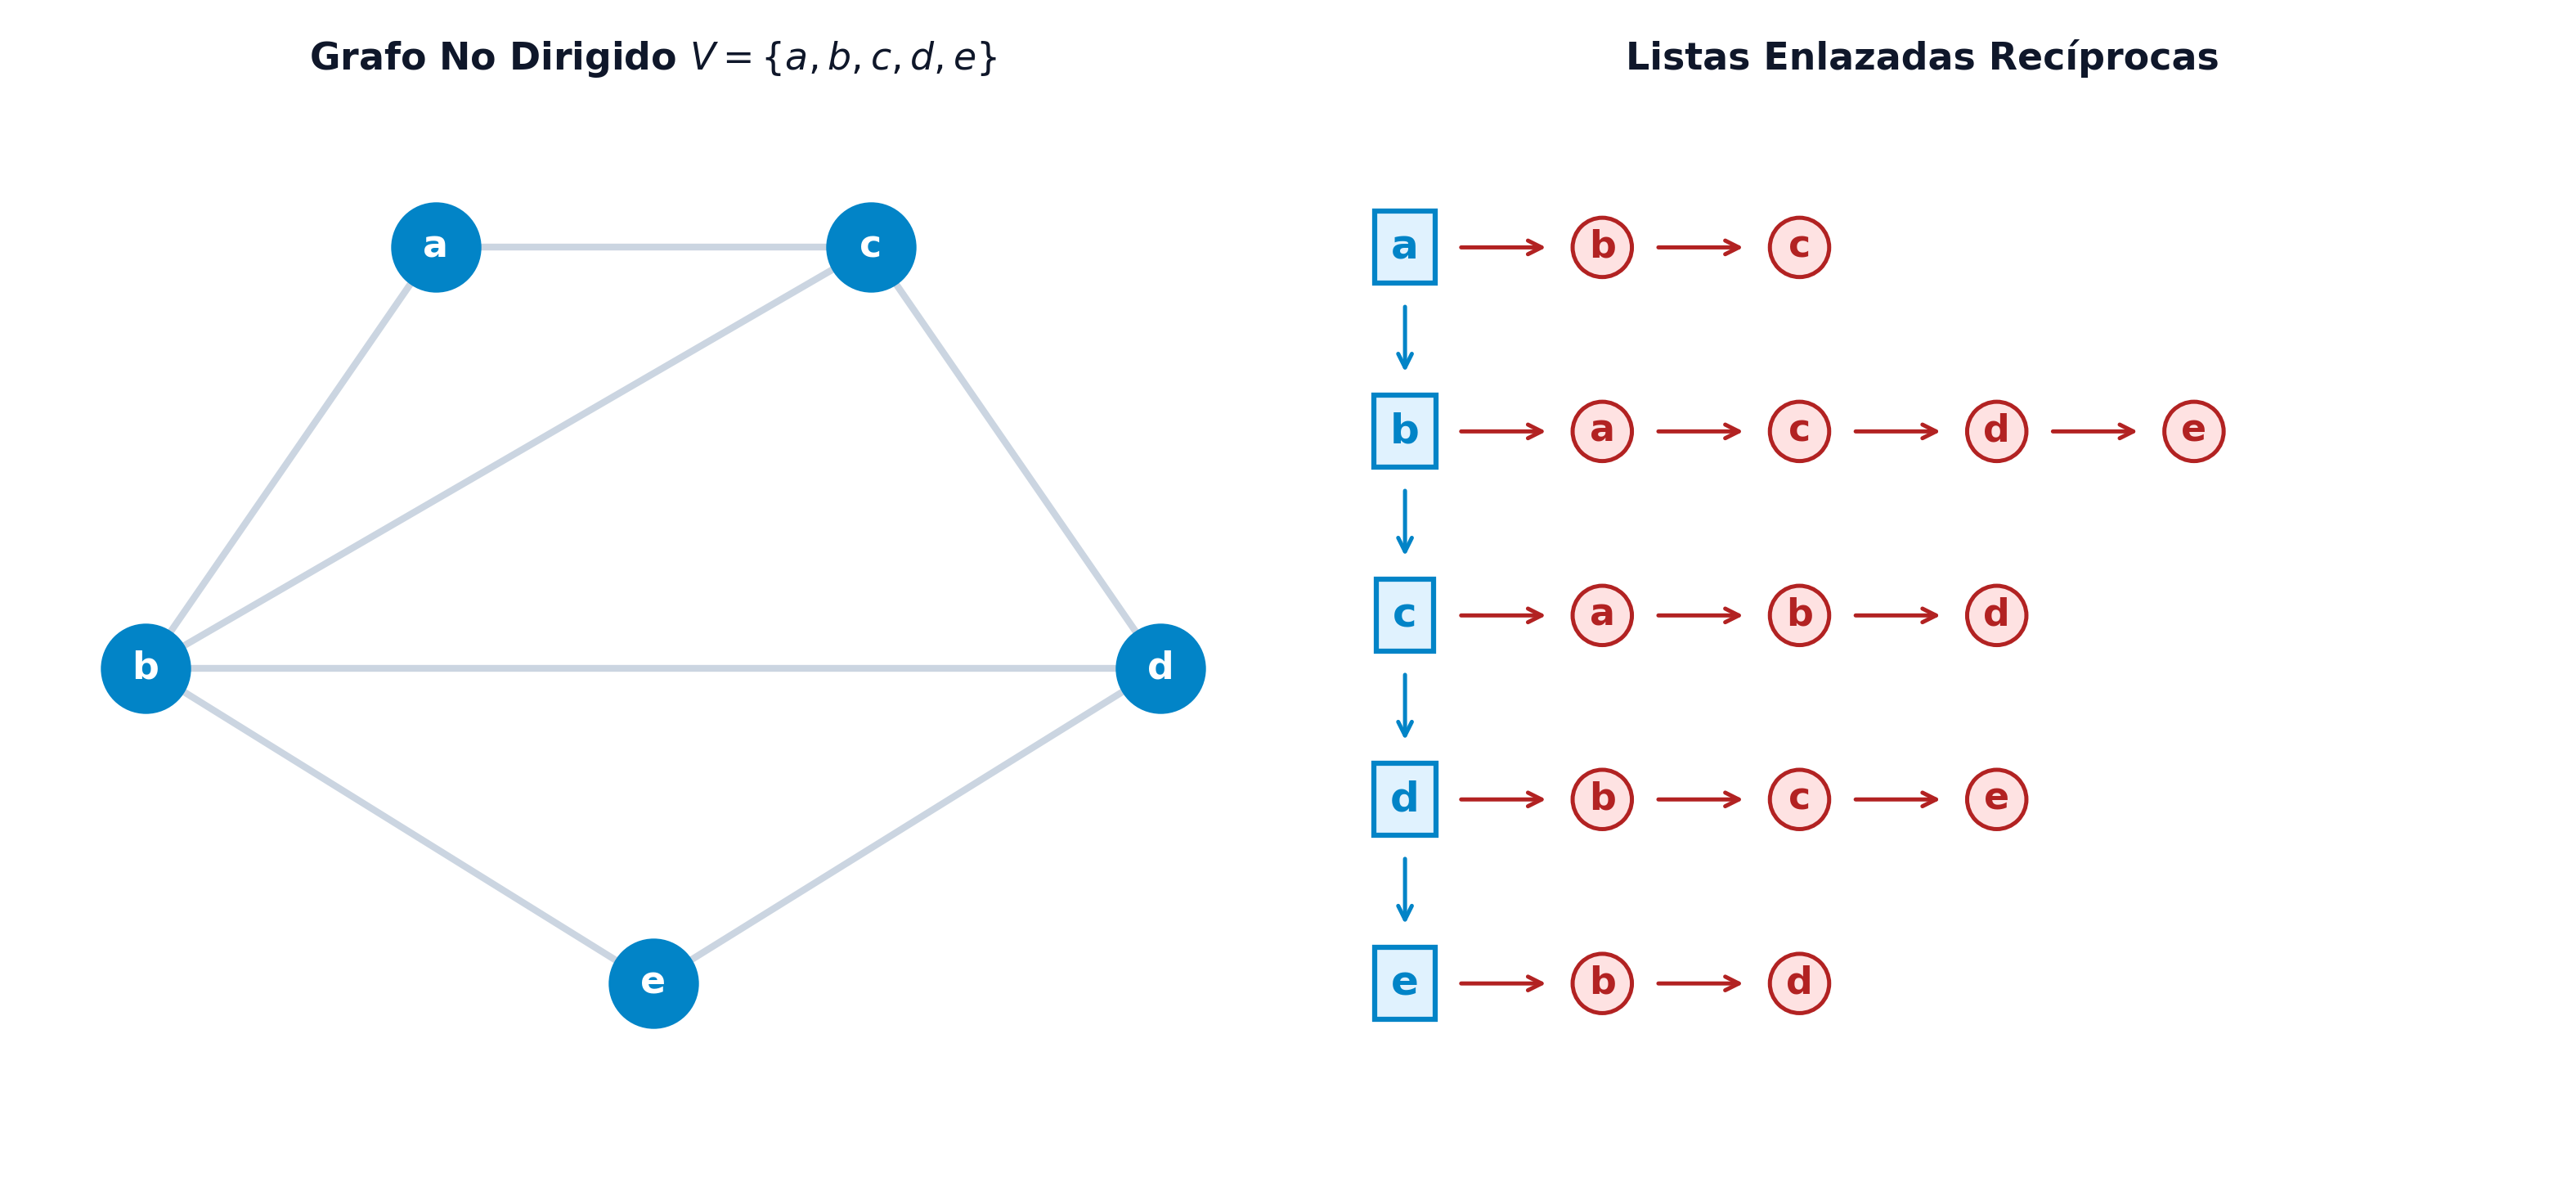
\includegraphics[keepaspectratio]{../images/lista_adyacencia_grafo.png}}
\end{column}
\end{columns}
\end{frame}

\section{Estructura matemática de los
árboles}\label{estructura-matemuxe1tica-de-los-uxe1rboles}

\begin{frame}{Definición de Árbol y Bosque}
\phantomsection\label{definiciuxf3n-de-uxe1rbol-y-bosque}
\begin{columns}[T]
\begin{column}{0.5\linewidth}
\begin{tcolorbox}[enhanced jigsaw, toptitle=1mm, opacityback=0, opacitybacktitle=0.6, colback=white, arc=.35mm, bottomrule=.15mm, titlerule=0mm, coltitle=black, breakable, bottomtitle=1mm, left=2mm, title=\textcolor{quarto-callout-note-color}{\faInfo}\hspace{0.5em}{Definición: Árbol y bosque}, colbacktitle=quarto-callout-note-color!10!white, rightrule=.15mm, toprule=.15mm, colframe=quarto-callout-note-color-frame, leftrule=.75mm]

\begin{itemize}
\tightlist
\item
  \textbf{Árbol}: Grafo no dirigido \textbf{conexo y acíclico}.
\item
  \textbf{Bosque}: Grafo acíclico cuyas componentes conexas son árboles.
\item
  \textbf{Matriz de incidencia}: Sus columnas son linealmente
  independientes.
\end{itemize}

\end{tcolorbox}
\end{column}

\begin{column}{0.5\linewidth}
\pandocbounded{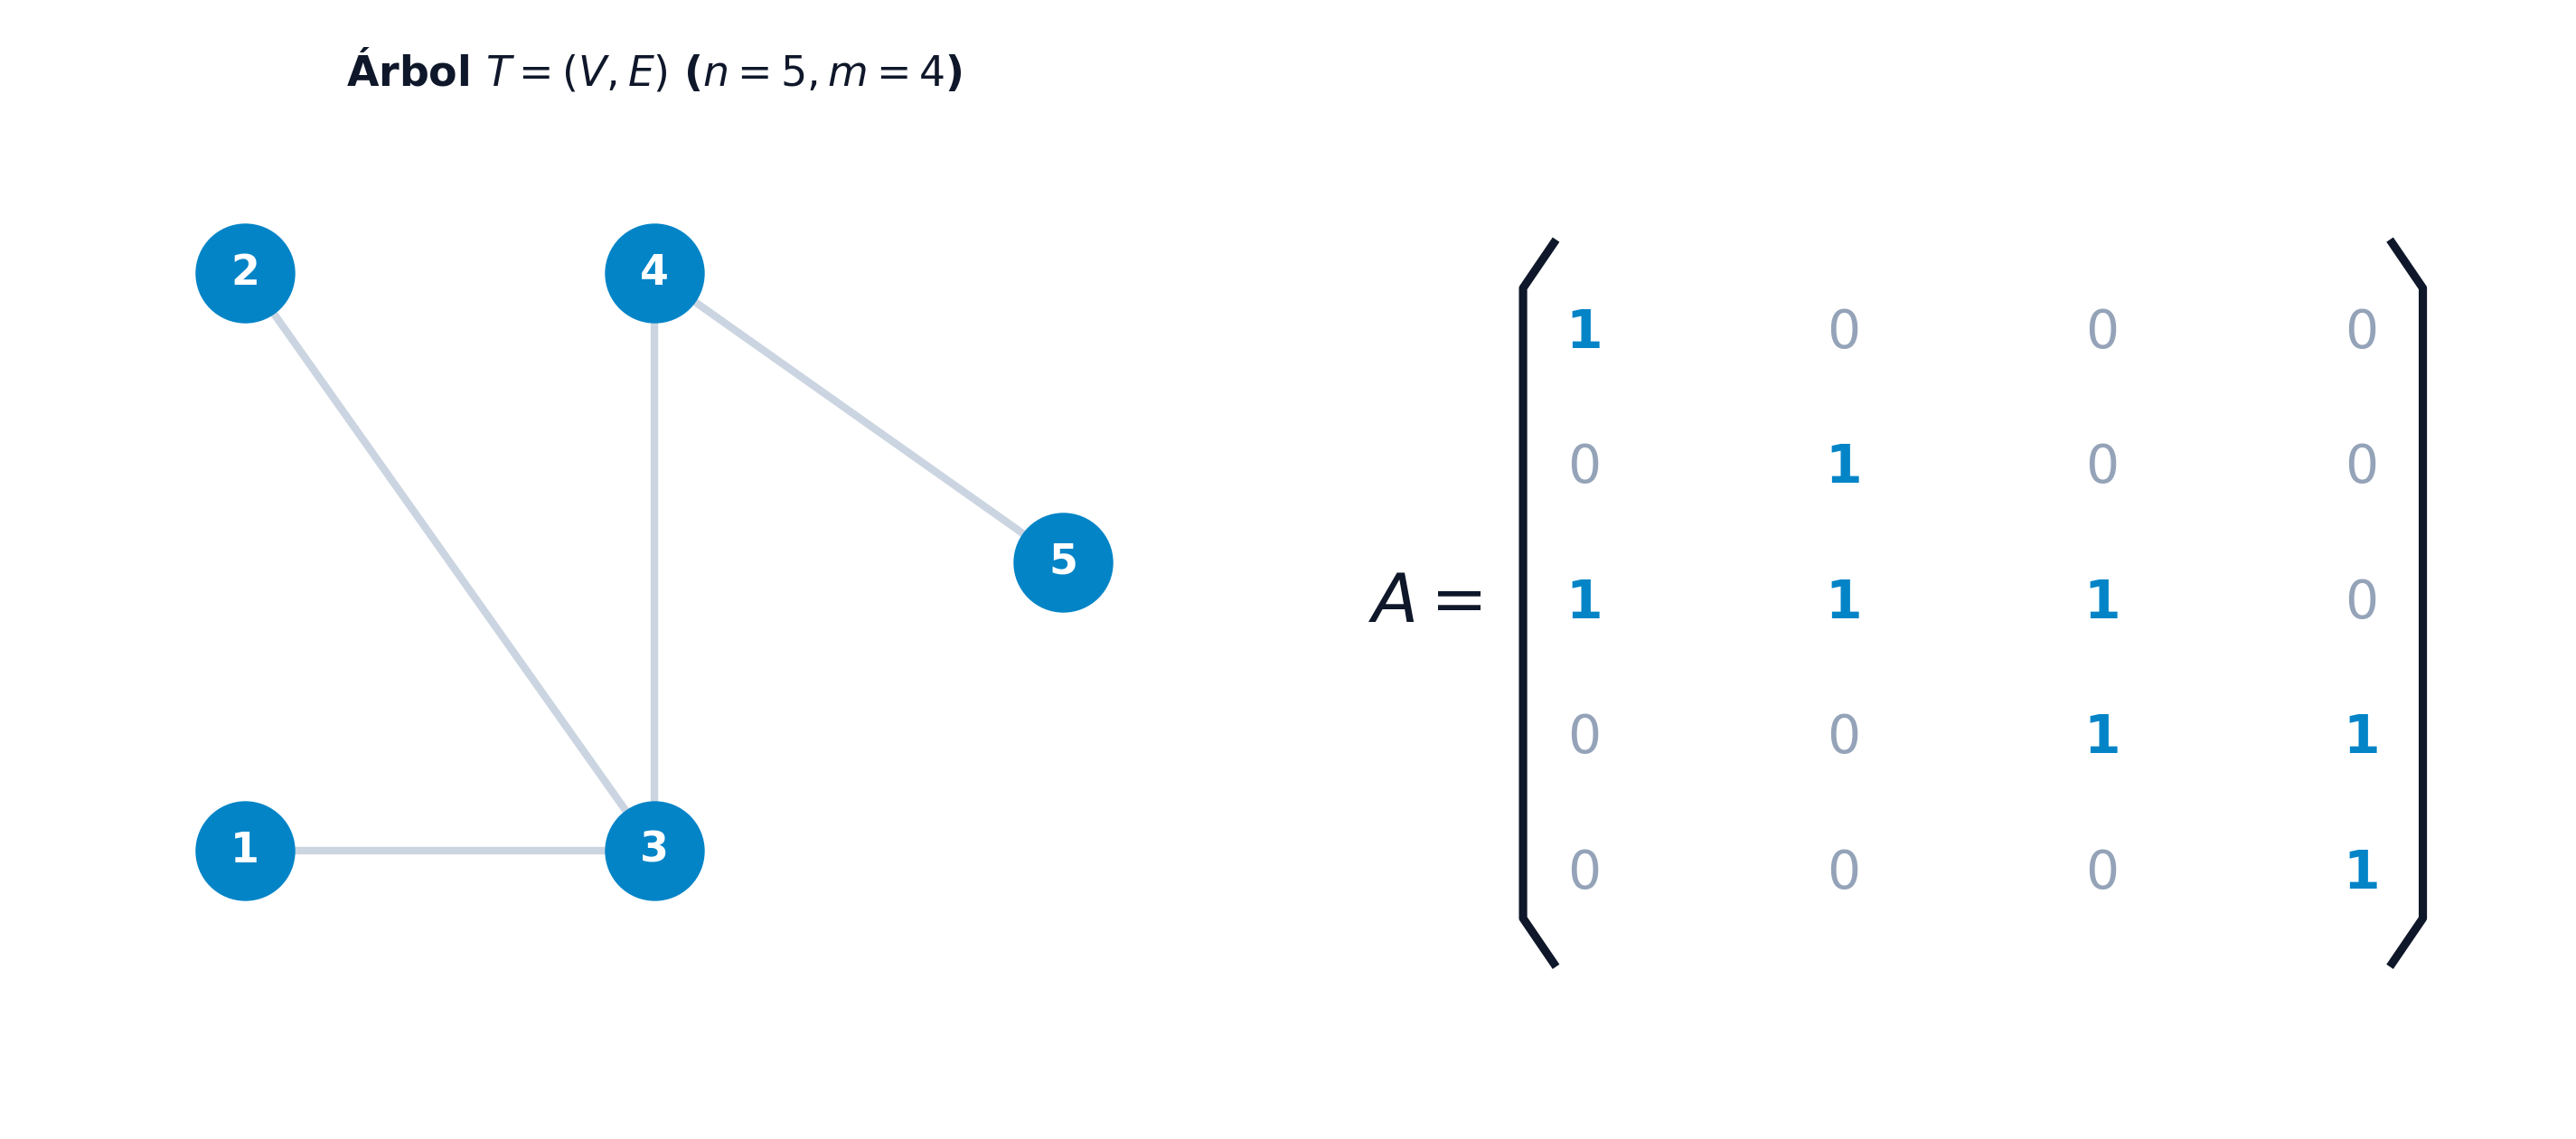
\includegraphics[keepaspectratio]{../images/arbol_ejemplo_matriz.png}}
\end{column}
\end{columns}
\end{frame}

\begin{frame}{Teorema: Caracterizaciones de un árbol (Parte 1)}
\phantomsection\label{teorema-caracterizaciones-de-un-uxe1rbol-parte-1}
\begin{tcolorbox}[enhanced jigsaw, toptitle=1mm, opacityback=0, opacitybacktitle=0.6, colback=white, arc=.35mm, bottomrule=.15mm, titlerule=0mm, coltitle=black, breakable, bottomtitle=1mm, left=2mm, title=\textcolor{quarto-callout-important-color}{\faExclamation}\hspace{0.5em}{Caracterizaciones equivalentes (1 a 3)}, colbacktitle=quarto-callout-important-color!10!white, rightrule=.15mm, toprule=.15mm, colframe=quarto-callout-important-color-frame, leftrule=.75mm]

Dado un grafo no dirigido \(G = (V, E)\) con \(n\) vértices y \(m\)
aristas, las siguientes propiedades son \textbf{equivalentes}:

\begin{enumerate}
\tightlist
\item
  \textbf{Conexo y acíclico}: \(G\) es un grafo conexo sin ningún ciclo.
\item
  \textbf{Acíclico maximal}: \(G\) es acíclico y al añadir una nueva
  arista entre cualquier par de vértices no adyacentes se crea
  \textbf{exactamente un ciclo}.
\item
  \textbf{Unicidad de cadenas}: Existe una \textbf{única cadena simple}
  entre todo par de vértices de \(G\).
\end{enumerate}

\end{tcolorbox}
\end{frame}

\begin{frame}{Teorema: Caracterizaciones de un árbol (Parte 2)}
\phantomsection\label{teorema-caracterizaciones-de-un-uxe1rbol-parte-2}
\begin{tcolorbox}[enhanced jigsaw, toptitle=1mm, opacityback=0, opacitybacktitle=0.6, colback=white, arc=.35mm, bottomrule=.15mm, titlerule=0mm, coltitle=black, breakable, bottomtitle=1mm, left=2mm, title=\textcolor{quarto-callout-important-color}{\faExclamation}\hspace{0.5em}{Caracterizaciones equivalentes (4 a 6)}, colbacktitle=quarto-callout-important-color!10!white, rightrule=.15mm, toprule=.15mm, colframe=quarto-callout-important-color-frame, leftrule=.75mm]

\begin{enumerate}
\setcounter{enumi}{3}
\tightlist
\item
  \textbf{Mínimamente conexo}: \(G\) es conexo y la eliminación de
  cualquier arista \textbf{lo desconecta} (\(G \setminus \{e\}\) no es
  conexo).
\item
  \textbf{Acíclico con \(m = n - 1\) aristas}: \(G\) es acíclico y el
  número de aristas satisface exactamente \(m = n - 1\).
\item
  \textbf{Conexo con \(m = n - 1\) aristas}: \(G\) es conexo y el número
  de aristas satisface exactamente \(m = n - 1\).
\end{enumerate}

\end{tcolorbox}
\end{frame}

\begin{frame}{Fórmula de Cayley y Vector de padres}
\phantomsection\label{fuxf3rmula-de-cayley-y-vector-de-padres}
\begin{columns}[T]
\begin{column}{0.5\linewidth}
\begin{itemize}
\item
  \textbf{Fórmula de Cayley (1889)}: El número de árboles soporte sobre
  \(n\) vértices es: \[
  T(n) = n^{n-2}
  \]
\item
  \textbf{Representación por Vector de Padres \(p(v)\)}: Al elegir una
  raíz \(x_0\), \(p(v)\) almacena el antecesor directo en la cadena
  desde \(x_0\). Ocupa solo \(n\) enteros.
\end{itemize}
\end{column}

\begin{column}{0.5\linewidth}
\pandocbounded{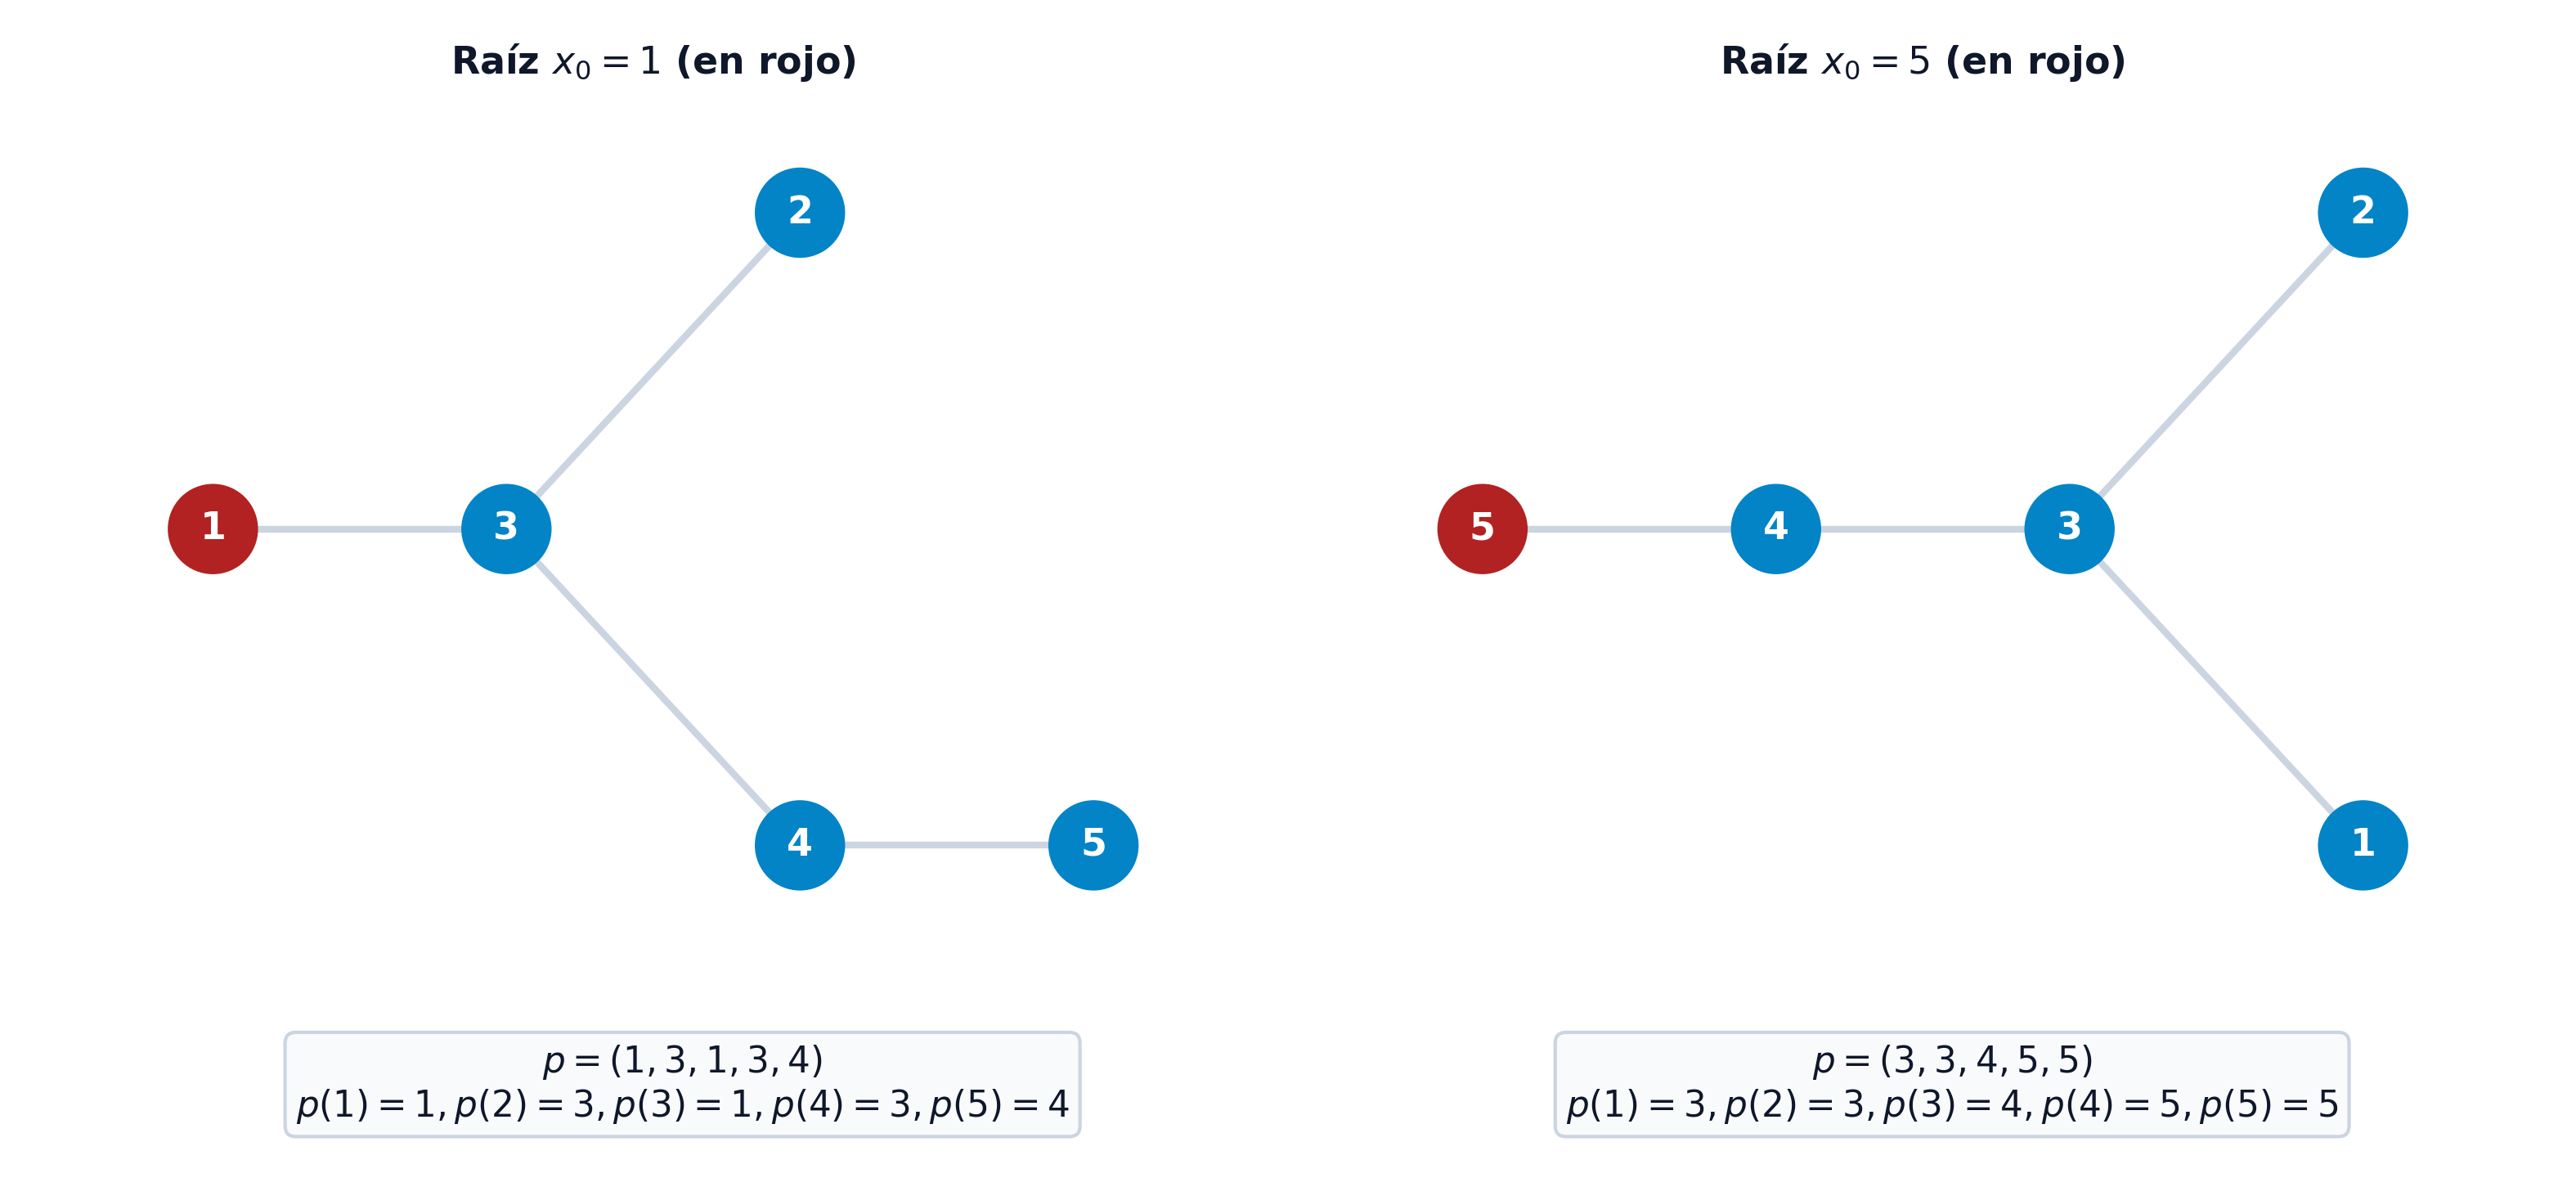
\includegraphics[keepaspectratio]{../images/arbol_vector_padres.png}}

\begin{itemize}
\tightlist
\item
  Izquierda: Raíz \(x_0 = 1 \implies p = (1, 3, 1, 3, 4)\).
\item
  Derecha: Raíz \(x_0 = 5 \implies p = (3, 3, 4, 5, 5)\).
\end{itemize}
\end{column}
\end{columns}
\end{frame}

\section{Árbol soporte de mínimo peso
(MST)}\label{uxe1rbol-soporte-de-muxednimo-peso-mst}

\begin{frame}{Redes valoradas: Definición y Notación}
\phantomsection\label{redes-valoradas-definiciuxf3n-y-notaciuxf3n}
\begin{tcolorbox}[enhanced jigsaw, toptitle=1mm, opacityback=0, opacitybacktitle=0.6, colback=white, arc=.35mm, bottomrule=.15mm, titlerule=0mm, coltitle=black, breakable, bottomtitle=1mm, left=2mm, title=\textcolor{quarto-callout-note-color}{\faInfo}\hspace{0.5em}{Definición: Red valorada y peso de aristas}, colbacktitle=quarto-callout-note-color!10!white, rightrule=.15mm, toprule=.15mm, colframe=quarto-callout-note-color-frame, leftrule=.75mm]

Una \textbf{red valorada} es un par \((G, \mathbf{d})\), donde
\(G = (V, E)\) o \(G = (V, U)\) es un grafo o digrafo y
\(\mathbf{d} \in \mathbb{R}^m\) es un vector cuyas componentes asignan
un coste o peso \(d(e) = d_e\) a cada arista \(e \in E\) (o \(c_{ij}\) a
cada arco \((i, j) \in U\)).

\end{tcolorbox}
\end{frame}

\begin{frame}{Formulación Primal del Problema del MST}
\phantomsection\label{formulaciuxf3n-primal-del-problema-del-mst}
\begin{tcolorbox}[enhanced jigsaw, toptitle=1mm, opacityback=0, opacitybacktitle=0.6, colback=white, arc=.35mm, bottomrule=.15mm, titlerule=0mm, coltitle=black, breakable, bottomtitle=1mm, left=2mm, title=\textcolor{quarto-callout-important-color}{\faExclamation}\hspace{0.5em}{Formulación Primal del Problema del MST}, colbacktitle=quarto-callout-important-color!10!white, rightrule=.15mm, toprule=.15mm, colframe=quarto-callout-important-color-frame, leftrule=.75mm]

Dada una red valorada conexa no dirigida \((G, \mathbf{d})\) con
\(G = (V, E)\) y pesos \(\{d_e : e \in E\}\), el \textbf{Problema del
Árbol Soporte de Mínimo Peso} (\emph{Minimum Spanning Tree}, MST) busca
un subconjunto de aristas \(T \subset E\) tal que \(H = (V, T)\) sea un
árbol soporte que minimice el peso acumulado: \[
\begin{aligned}
\min_{T \subset E} \quad & d(T) = \sum_{e \in T} d_e \\
\text{sujeto a} \quad & H = (V, T) \text{ es un árbol soporte de } G
\end{aligned}
\]

\end{tcolorbox}
\end{frame}

\begin{frame}{Ejemplo: Espacio de soluciones del MST}
\phantomsection\label{ejemplo-espacio-de-soluciones-del-mst}
\begin{center}
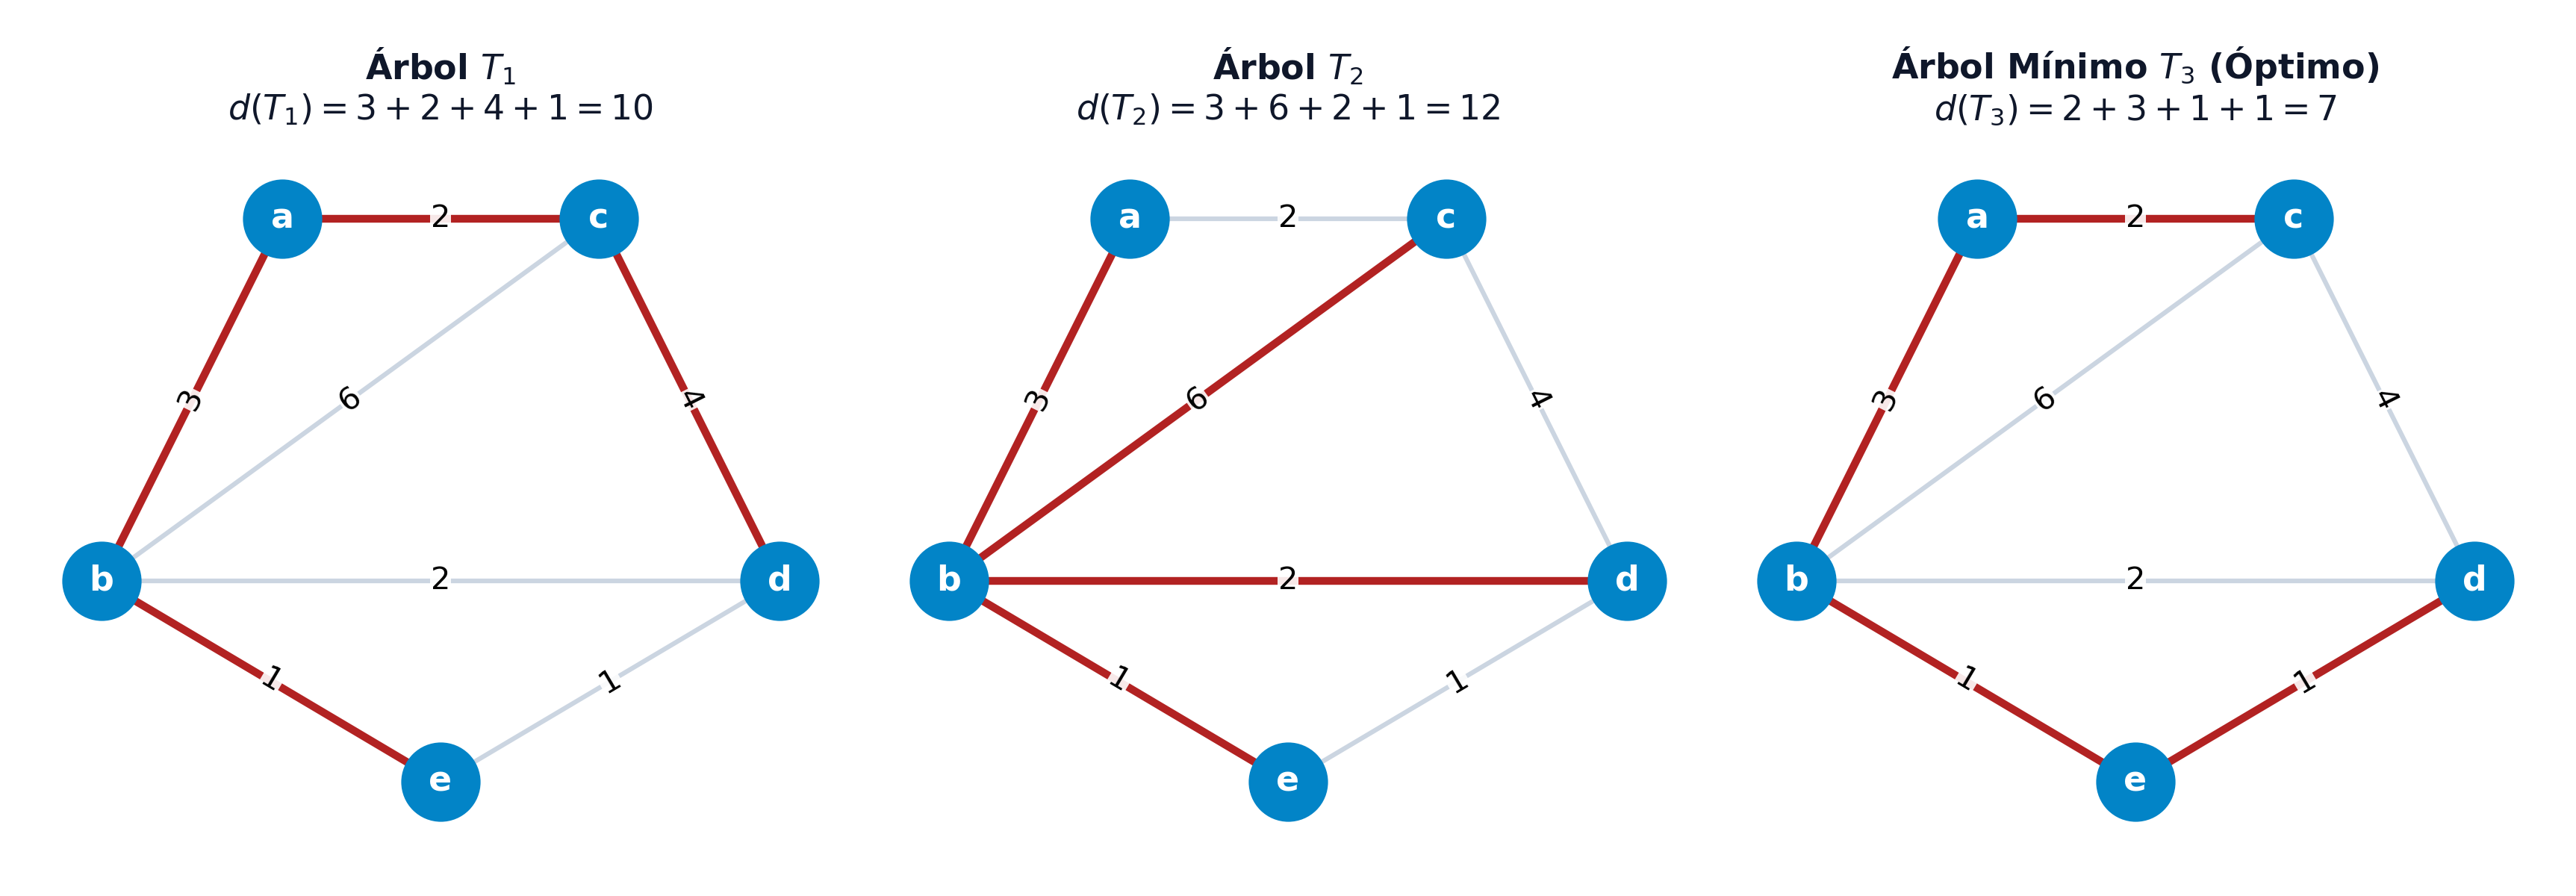
\includegraphics[width=0.85\linewidth,height=\textheight,keepaspectratio]{../images/mst_ejemplo_tres_arboles.png}
\end{center}

\begin{itemize}
\tightlist
\item
  Comparación de tres árboles soporte candidatos sobre una red no
  dirigida de 5 vértices \(V = \{a, b, c, d, e\}\).
\end{itemize}
\end{frame}

\begin{frame}{Ejemplo: Evaluación de coste en árboles candidatos}
\phantomsection\label{ejemplo-evaluaciuxf3n-de-coste-en-uxe1rboles-candidatos}
Evaluación de pesos acumulados sobre la red de 5 vértices:

\begin{itemize}
\tightlist
\item
  \textbf{Candidato \(T_1\)} (\(\{a,b\}, \{a,c\}, \{c,d\}, \{b,e\}\)):
  \[d(T_1) = 3 + 2 + 4 + 1 = 10\]
\item
  \textbf{Candidato \(T_2\)} (\(\{a,b\}, \{b,c\}, \{b,d\}, \{b,e\}\)):
  \[d(T_2) = 3 + 6 + 2 + 1 = 12\]
\item
  \textbf{Árbol Mínimo \(T_3\) (Óptimo)}
  (\(\{a,c\}, \{a,b\}, \{b,e\}, \{e,d\}\)):
  \[d(T_3) = 2 + 3 + 1 + 1 = 7\]
\end{itemize}
\end{frame}

\begin{frame}{Teorema: Propiedad del Corte (Cut Property)}
\phantomsection\label{teorema-propiedad-del-corte-cut-property}
\begin{tcolorbox}[enhanced jigsaw, toptitle=1mm, opacityback=0, opacitybacktitle=0.6, colback=white, arc=.35mm, bottomrule=.15mm, titlerule=0mm, coltitle=black, breakable, bottomtitle=1mm, left=2mm, title=\textcolor{quarto-callout-important-color}{\faExclamation}\hspace{0.5em}{Teorema: Propiedad del Corte (Cut Property)}, colbacktitle=quarto-callout-important-color!10!white, rightrule=.15mm, toprule=.15mm, colframe=quarto-callout-important-color-frame, leftrule=.75mm]

Sea \((G, \mathbf{d})\) una red valorada conexa no dirigida. Dado
cualquier subconjunto propio de vértices \(S \subset V\), si la arista
\(e^* = \{u, v\}\) con \(u \in S, v \in V \setminus S\) es la arista de
\textbf{peso estrictamente mínimo} que cruza el corte \(w(S)\), entonces
la arista \(e^*\) \textbf{pertenece obligatoriamente a todo Árbol
Soporte de Mínimo Peso} de \(G\).

\end{tcolorbox}

\begin{itemize}
\tightlist
\item
  \textbf{Fundamento algorítmico}: La propiedad del corte permite tomar
  decisiones locales óptimas (\emph{golosas}) sin necesidad de evaluar
  la cantidad exponencial de árboles soporte (\(T(n) = n^{n-2}\)).
\end{itemize}
\end{frame}

\begin{frame}{Algoritmo de Kruskal: Estrategia Golosa}
\phantomsection\label{algoritmo-de-kruskal-estrategia-golosa}
\begin{tcolorbox}[enhanced jigsaw, toptitle=1mm, opacityback=0, opacitybacktitle=0.6, colback=white, arc=.35mm, bottomrule=.15mm, titlerule=0mm, coltitle=black, breakable, bottomtitle=1mm, left=2mm, title=\textcolor{quarto-callout-note-color}{\faInfo}\hspace{0.5em}{Filosofía del Algoritmo de Kruskal (1956)}, colbacktitle=quarto-callout-note-color!10!white, rightrule=.15mm, toprule=.15mm, colframe=quarto-callout-note-color-frame, leftrule=.75mm]

\begin{itemize}
\tightlist
\item
  Propuesto por Joseph Kruskal (1956), adopta una \textbf{estrategia
  golosa (\emph{greedy}) global} centrada en el ordenamiento de las
  aristas.
\item
  Examina secuencialmente las aristas de la red en orden creciente de
  peso e incorpora a la solución parcial la arista disponible de menor
  coste, siempre que \textbf{no genere ningún ciclo} con las aristas
  previamente seleccionadas.
\end{itemize}

\end{tcolorbox}

\begin{itemize}
\tightlist
\item
  \textbf{Bosque disjunto parcial}: En las fases intermedias, las
  aristas en \(T\) no forman una estructura conexa continua, sino un
  \textbf{bosque parcial de árboles disjuntos} que se fusionan
  progresivamente hasta alcanzar \(|T| = n - 1\) aristas.
\end{itemize}
\end{frame}

\begin{frame}{Esquema de Kruskal: Inicialización y Selección}
\phantomsection\label{esquema-de-kruskal-inicializaciuxf3n-y-selecciuxf3n}
Dada una red no dirigida valorada \(G = (V, E, \mathbf{d})\) con
\(n = |V| > 1\) vértices:

\begin{itemize}
\tightlist
\item
  \textbf{Paso 0 (Inicialización)}:

  \begin{itemize}
  \tightlist
  \item
    Definir \(T = \emptyset\) y conjunto de aristas disponibles
    \(A \leftarrow E\).
  \end{itemize}
\item
  \textbf{Paso 1 (Bucle de Selección Golosa)}:

  \begin{itemize}
  \tightlist
  \item
    Mientras \(|T| < n - 1\) y \(A \neq \emptyset\):

    \begin{enumerate}
    \tightlist
    \item
      Identificar la arista \(e \in A\) de menor peso global.
    \item
      Actualizar el conjunto de disponibles:
      \(A \leftarrow A \setminus \{e\}\).
    \item
      Si el subconjunto \(T \cup \{e\}\) \textbf{no contiene ningún
      ciclo}, aceptar: \(T \leftarrow T \cup \{e\}\).
    \end{enumerate}
  \end{itemize}
\end{itemize}
\end{frame}

\begin{frame}{Esquema de Kruskal: Criterio de Parada}
\phantomsection\label{esquema-de-kruskal-criterio-de-parada}
\begin{itemize}
\item
  \textbf{Paso 2 (Criterio de Parada y Verificación)}:

  \begin{itemize}
  \item
    \textbf{Éxito}: Si \(|T| = n - 1\), el par \(H = (V, T)\) es un
    \textbf{Árbol Soporte de Mínimo Peso (MST)}.
  \item
    \textbf{Desconexión}: Si \(A = \emptyset\) y \(|T| < n - 1\), la red
    \(G\) no era conexa, obteniéndose el bosque soporte de mínimo peso
    de sus componentes conexas.
  \end{itemize}
\end{itemize}
\end{frame}

\begin{frame}{Estructura Union-Find y Complejidad de Kruskal}
\phantomsection\label{estructura-union-find-y-complejidad-de-kruskal}
\begin{columns}[T]
\begin{column}{0.5\linewidth}
\begin{tcolorbox}[enhanced jigsaw, toptitle=1mm, opacityback=0, opacitybacktitle=0.6, colback=white, arc=.35mm, bottomrule=.15mm, titlerule=0mm, coltitle=black, breakable, bottomtitle=1mm, left=2mm, title=\textcolor{quarto-callout-note-color}{\faInfo}\hspace{0.5em}{Detección de ciclos con Union-Find}, colbacktitle=quarto-callout-note-color!10!white, rightrule=.15mm, toprule=.15mm, colframe=quarto-callout-note-color-frame, leftrule=.75mm]

\begin{itemize}
\tightlist
\item
  Cada vértice inicia en su propio bloque disjunto:
  \(S_k = \{k\}, \forall k \in V\).
\item
  Para cada arista \(e = \{i, j\}\), se consulta \(\text{Find}(i)\) y
  \(\text{Find}(j)\).
\item
  Si \(\text{Find}(i) \neq \text{Find}(j)\), \textbf{no hay ciclo}: se
  acepta la arista en \(T\) y se ejecuta \(\text{Union}(S(i), S(j))\).
\item
  Si \(\text{Find}(i) = \text{Find}(j)\), la arista se descarta.
\end{itemize}

\end{tcolorbox}
\end{column}

\begin{column}{0.5\linewidth}
\begin{tcolorbox}[enhanced jigsaw, toptitle=1mm, opacityback=0, opacitybacktitle=0.6, colback=white, arc=.35mm, bottomrule=.15mm, titlerule=0mm, coltitle=black, breakable, bottomtitle=1mm, left=2mm, title=\textcolor{quarto-callout-note-color}{\faInfo}\hspace{0.5em}{Complejidad computacional}, colbacktitle=quarto-callout-note-color!10!white, rightrule=.15mm, toprule=.15mm, colframe=quarto-callout-note-color-frame, leftrule=.75mm]

\begin{itemize}
\tightlist
\item
  \textbf{Preordenación de aristas}: Ordenar las \(m\) aristas requiere
  \(O(m \log m)\).
\item
  Dado que \(m \le n^2 \implies \log m \le 2 \log n\).
\item
  \textbf{Complejidad total}: \textbf{\(O(m \log n)\)} o
  \(O(m \cdot \alpha(n))\) si las aristas están preordenadas.
\end{itemize}

\end{tcolorbox}
\end{column}
\end{columns}
\end{frame}

\begin{frame}{Ejemplo Kruskal: Red de 6 vértices y Matriz de pesos}
\phantomsection\label{ejemplo-kruskal-red-de-6-vuxe9rtices-y-matriz-de-pesos}
\begin{itemize}
\tightlist
\item
  \textbf{Planteamiento}: Obtener el MST mediante el Algoritmo de
  Kruskal para una red no dirigida de \(n = 6\) vértices y 11 aristas
  valoradas con costes entre \(d=1\) y \(d=10\).
\item
  \textbf{Topología y Matriz simétrica de pesos
  \(B \in \mathbb{R}^{6 \times 6}\)}:
\end{itemize}

\begin{center}
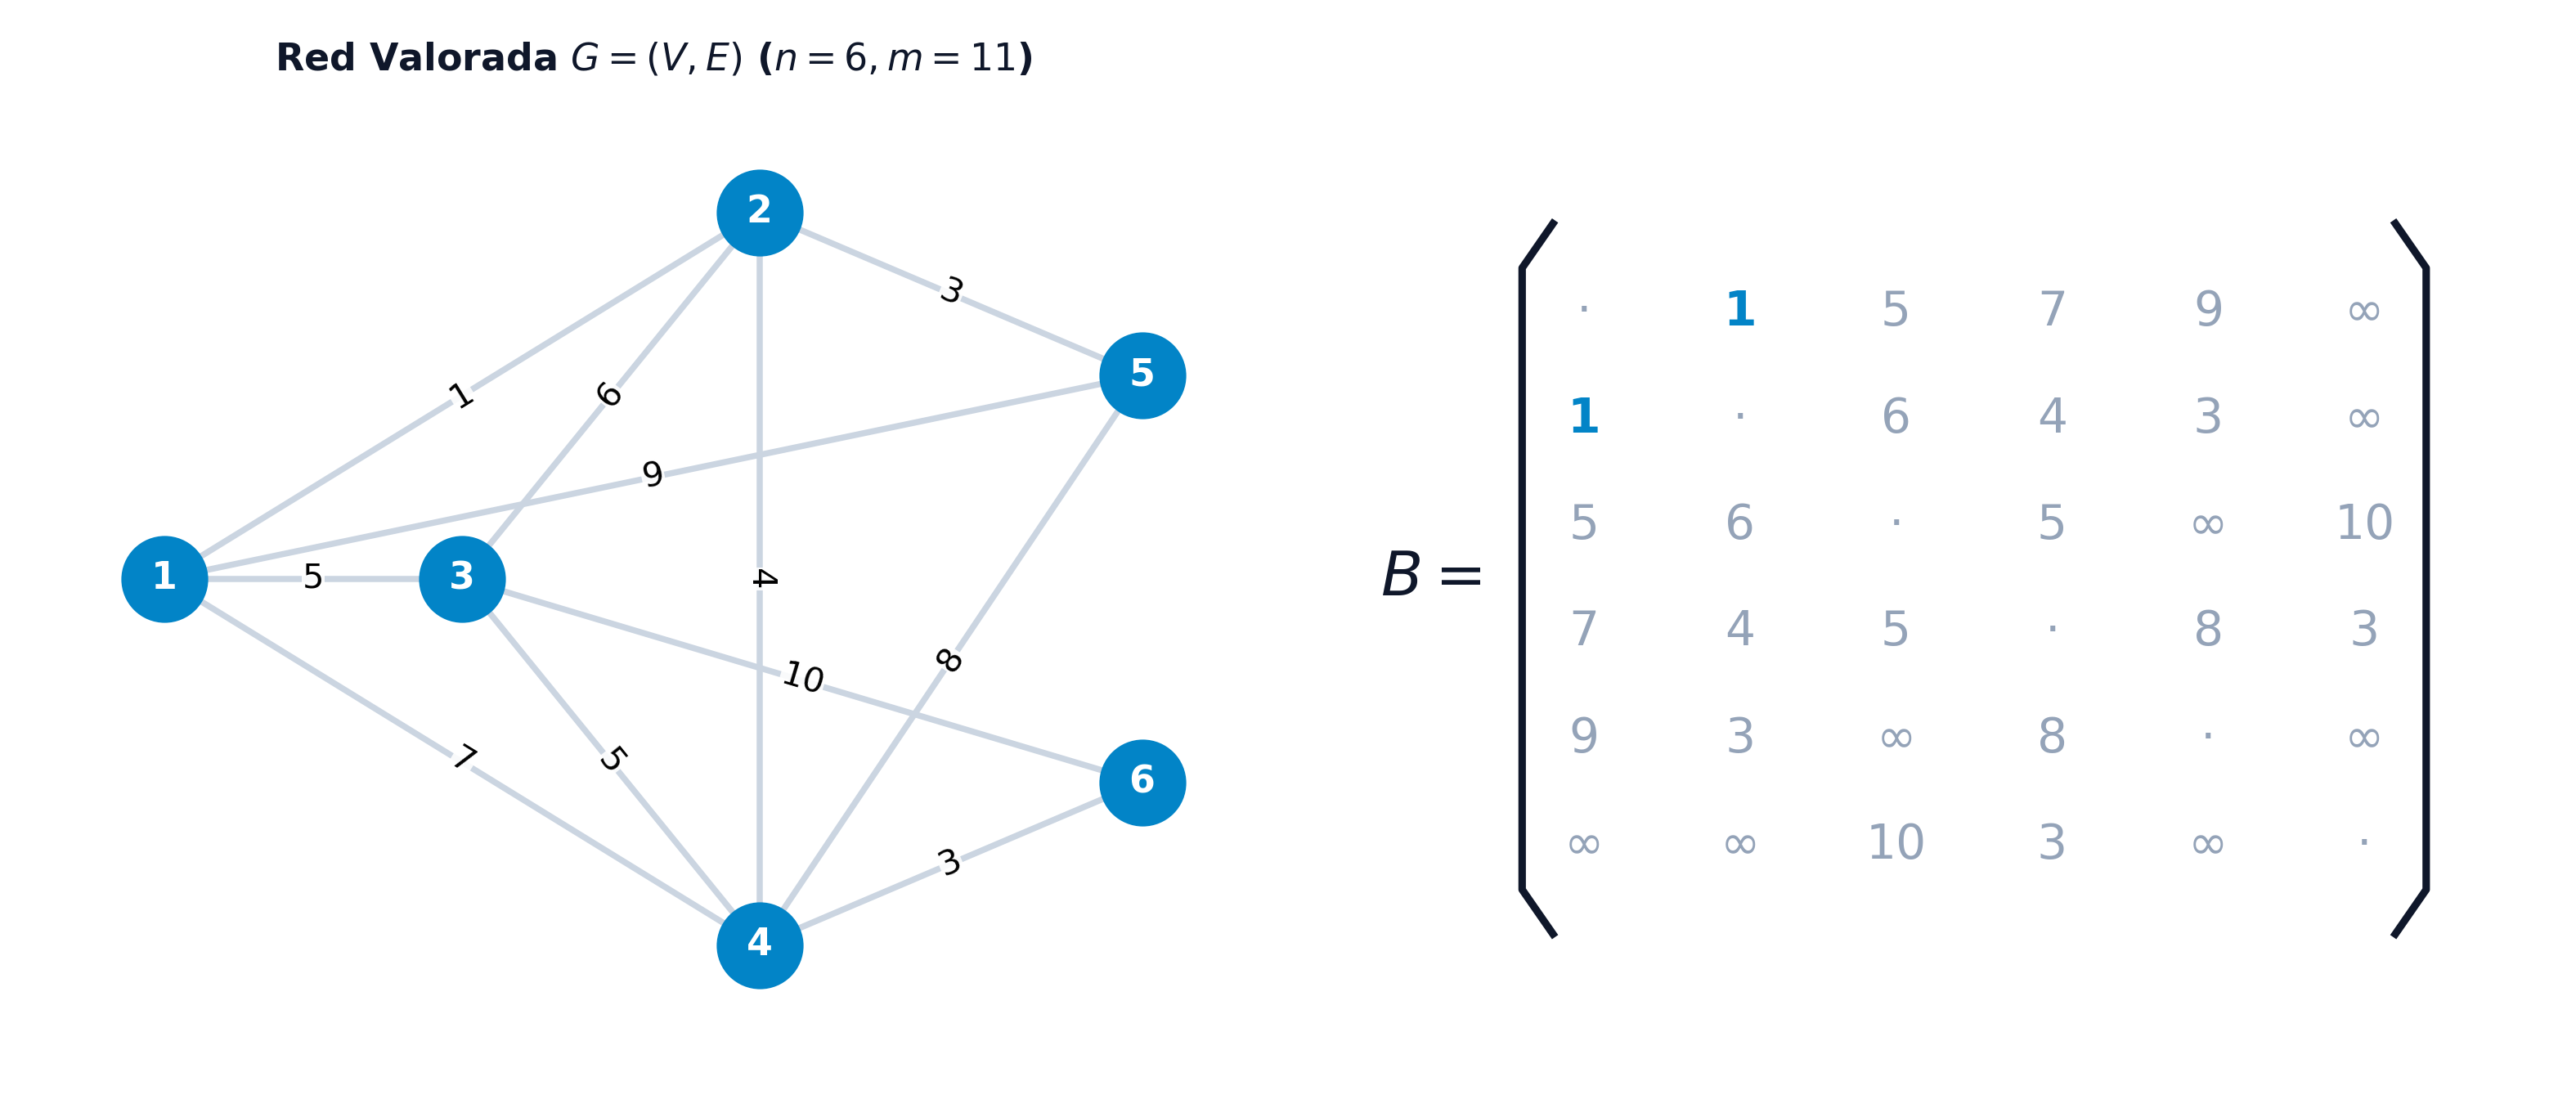
\includegraphics[width=0.85\linewidth,height=\textheight,keepaspectratio]{../images/kruskal_ejemplo_matriz.png}
\end{center}
\end{frame}

\begin{frame}{Ejemplo Kruskal: Estado inicial (\(k=0\))}
\phantomsection\label{ejemplo-kruskal-estado-inicial-k0}
\begin{itemize}
\item
  \textbf{Vértices de la red}: \(V = \{1, 2, 3, 4, 5, 6\}\) (\(n=6\)).
\item
  \textbf{Árbol parcial vacíos}: \(T = \emptyset\).
\item
  \textbf{Estructura de subconjuntos disjuntos iniciales}: \[
  \{1\}, \, \{2\}, \, \{3\}, \, \{4\}, \, \{5\}, \, \{6\}
  \]
\item
  \textbf{Aristas candidatas ordenadas por peso creciente}:

  \begin{enumerate}
  \tightlist
  \item
    \(\{1, 2\}\) (\(d=1\))
  \item
    \(\{2, 5\}\) (\(d=3\)), \(\{4, 6\}\) (\(d=3\))
  \item
    \(\{2, 4\}\) (\(d=4\))
  \item
    \(\{1, 3\}\) (\(d=5\)), \(\{3, 4\}\) (\(d=5\))
  \item
    \(\{2, 3\}\) (\(d=6\)), \(\{1, 4\}\) (\(d=7\)), \(\{4, 5\}\)
    (\(d=8\)), \(\{1, 5\}\) (\(d=9\)), \(\{3, 5\}\) (\(d=9\)),
    \(\{3, 6\}\) (\(d=10\))
  \end{enumerate}
\end{itemize}
\end{frame}

\begin{frame}{Ejemplo Kruskal: Iteración 1 (\(k=1, d=1\))}
\phantomsection\label{ejemplo-kruskal-iteraciuxf3n-1-k1-d1}
\begin{itemize}
\item
  \textbf{Selección de la arista de menor peso global}:
  \(e_1 = \{1, 2\}\) con \(d_{\{1,2\}} = 1\).
\item
  \textbf{Consulta Union-Find}:
  \(\text{Find}(1) \neq \text{Find}(2) \implies \{1\} \neq \{2\}\).
\item
  \textbf{Actualización del árbol parcial}:

  \begin{itemize}
  \tightlist
  \item
    \(T = \{\{1, 2\}\}\).
  \item
    Subconjuntos disjuntos fusionados: \[
    \{1, 2\}, \, \{3\}, \, \{4\}, \, \{5\}, \, \{6\}
    \]
  \end{itemize}
\end{itemize}
\end{frame}

\begin{frame}{Ejemplo Kruskal: Iteraciones 2 y 3 (\(d=3\), empates)}
\phantomsection\label{ejemplo-kruskal-iteraciones-2-y-3-d3-empates}
\begin{itemize}
\tightlist
\item
  \textbf{Iteración \(k=2\) (\(d=3\))}:

  \begin{itemize}
  \tightlist
  \item
    Candidatas de peso 3: \(\{2, 5\}\) y \(\{4, 6\}\). Seleccionar
    \(\{2, 5\}\).
  \item
    \(\text{Find}(2) \neq \text{Find}(5) \implies\) Aceptar
    \(\{2, 5\}\).
  \item
    \(T = \{\{1, 2\}, \{2, 5\}\}\).
  \item
    Subconjuntos: \(\{1, 2, 5\}, \, \{3\}, \, \{4\}, \, \{6\}\).
  \end{itemize}
\item
  \textbf{Iteración \(k=3\) (\(d=3\))}:

  \begin{itemize}
  \tightlist
  \item
    Seleccionar la arista \(\{4, 6\}\) de peso 3.
  \item
    \(\text{Find}(4) \neq \text{Find}(6) \implies\) Aceptar
    \(\{4, 6\}\).
  \item
    \(T = \{\{1, 2\}, \{2, 5\}, \{4, 6\}\}\).
  \item
    Subconjuntos: \(\{1, 2, 5\}, \, \{3\}, \, \{4, 6\}\).
  \end{itemize}
\end{itemize}
\end{frame}

\begin{frame}{Ejemplo Kruskal: Iteraciones 4 y 5 (\(d=4, d=5\))}
\phantomsection\label{ejemplo-kruskal-iteraciones-4-y-5-d4-d5}
\begin{itemize}
\tightlist
\item
  \textbf{Iteración \(k=4\) (\(d=4\))}:

  \begin{itemize}
  \tightlist
  \item
    Arista \(\{2, 4\}\) de peso 4.
  \item
    \(\text{Find}(2) \in \{1, 2, 5\}\) y
    \(\text{Find}(4) \in \{4, 6\} \implies\) Componentes distintas, no
    forma ciclo.
  \item
    \(T = \{\{1, 2\}, \{2, 5\}, \{4, 6\}, \{2, 4\}\}\).
  \item
    Subconjuntos: \(\{1, 2, 4, 5, 6\}, \, \{3\}\).
  \end{itemize}
\item
  \textbf{Iteración \(k=5\) (\(d=5\), empate con \(\{3,4\}\))}:

  \begin{itemize}
  \tightlist
  \item
    Arista \(\{1, 3\}\) de peso 5.
  \item
    \(\text{Find}(1) \in \{1, 2, 4, 5, 6\}\) y
    \(\text{Find}(3) \in \{3\} \implies\) Aceptar \(\{1, 3\}\).
  \item
    \(T = \{\{1, 2\}, \{2, 5\}, \{4, 6\}, \{2, 4\}, \{1, 3\}\}\).
  \item
    Subconjuntos: \(\{1, 2, 3, 4, 5, 6\}\) (1 sola componente conexa).
  \end{itemize}
\end{itemize}
\end{frame}

\begin{frame}{Ejemplo Kruskal: Conclusión y Peso Mínimo}
\phantomsection\label{ejemplo-kruskal-conclusiuxf3n-y-peso-muxednimo}
\begin{itemize}
\item
  \textbf{Criterio de parada}: Se alcanzan exactamente
  \(|T| = n - 1 = 5\) aristas en la solución parcial.
\item
  \textbf{Cálculo del Peso Óptimo Acumulado}: \[
  \begin{aligned}
  d(T) &= d_{\{1,2\}} + d_{\{2,5\}} + d_{\{4,6\}} + d_{\{2,4\}} + d_{\{1,3\}} \\
       &= 1 + 3 + 3 + 4 + 5 = 16
  \end{aligned}
  \]
\item
  \textbf{Árbol Soporte Mínimo resultado}: \(H = (V, T)\) con
  \(T = \{\{1, 2\}, \{2, 5\}, \{4, 6\}, \{2, 4\}, \{1, 3\}\}\).
\end{itemize}
\end{frame}

\begin{frame}{Ejemplo Kruskal: Solución Óptima Alternativa \(T'\)}
\phantomsection\label{ejemplo-kruskal-soluciuxf3n-uxf3ptima-alternativa-t}
\begin{itemize}
\item
  \textbf{Resolución de empate en \(k=5\)}: En la iteración 5 existía un
  empate entre \(\{1, 3\}\) (\(d=5\)) y \(\{3, 4\}\) (\(d=5\)).
\item
  \textbf{Árbol Soporte Mínimo Alternativo \(T'\)}: Si se hubiese
  seleccionado \(\{3, 4\}\) en lugar de \(\{1, 3\}\): \[
  T' = \{\{1, 2\}, \{2, 5\}, \{4, 6\}, \{2, 4\}, \{3, 4\}\}
  \]
\item
  \textbf{Peso del árbol alternativo}:
  \[d(T') = 1 + 3 + 3 + 4 + 5 = 16\]
\item
  \textbf{Conclusión}: Cuando existen pesos duplicados, el árbol mínimo
  \textbf{puede no ser único}, aunque el peso óptimo \(d(T)\) es siempre
  constante e invariable.
\end{itemize}
\end{frame}

\begin{frame}{Ejemplo Kruskal: Traza animada interactiva}
\phantomsection\label{ejemplo-kruskal-traza-animada-interactiva}
\end{frame}

\begin{frame}{Complejidad del Algoritmo de Kruskal}
\phantomsection\label{complejidad-del-algoritmo-de-kruskal}
\begin{tcolorbox}[enhanced jigsaw, toptitle=1mm, opacityback=0, opacitybacktitle=0.6, colback=white, arc=.35mm, bottomrule=.15mm, titlerule=0mm, coltitle=black, breakable, bottomtitle=1mm, left=2mm, title=\textcolor{quarto-callout-note-color}{\faInfo}\hspace{0.5em}{Complejidad computacional de Kruskal}, colbacktitle=quarto-callout-note-color!10!white, rightrule=.15mm, toprule=.15mm, colframe=quarto-callout-note-color-frame, leftrule=.75mm]

\begin{itemize}
\tightlist
\item
  \textbf{Sin ordenación previa de aristas}:
  \(O(m \log m) = O(m \log n)\).
\item
  \textbf{Con aristas preordenadas}: \(O(m \cdot \alpha(n))\) (casi
  lineal mediante compresión de caminos en Union-Find).
\end{itemize}

\end{tcolorbox}
\end{frame}

\begin{frame}{Algoritmo de Prim (Jarník-Prim-Dijkstra)}
\phantomsection\label{algoritmo-de-prim-jarnuxedk-prim-dijkstra}
\begin{tcolorbox}[enhanced jigsaw, toptitle=1mm, opacityback=0, opacitybacktitle=0.6, colback=white, arc=.35mm, bottomrule=.15mm, titlerule=0mm, coltitle=black, breakable, bottomtitle=1mm, left=2mm, title=\textcolor{quarto-callout-note-color}{\faInfo}\hspace{0.5em}{Historia y Filosofía del Algoritmo de Prim (1957)}, colbacktitle=quarto-callout-note-color!10!white, rightrule=.15mm, toprule=.15mm, colframe=quarto-callout-note-color-frame, leftrule=.75mm]

\begin{itemize}
\tightlist
\item
  Descubierto por Vojtěch Jarník (1930), redescubierto por Robert C.
  Prim (1957) y Edsger W. Dijkstra (1959).
\item
  A diferencia de Kruskal (que gestiona un bosque inconexo), Prim hace
  crecer \textbf{una única arborescencia conexa continua} desde un nodo
  raíz inicial \(v_1 \in V\).
\end{itemize}

\end{tcolorbox}

\begin{itemize}
\tightlist
\item
  \textbf{Corte de la arborescencia}: Sea \(P \subset V\) los nodos ya
  integrados (\(P = \{v_1\}\) inicialmente) y \(N = V \setminus P\) los
  nodos pendientes. En cada iteración se selecciona la arista de peso
  mínimo del corte \(w(P)\).
\end{itemize}
\end{frame}

\begin{frame}{Esquema de Prim: Inicialización y Selección}
\phantomsection\label{esquema-de-prim-inicializaciuxf3n-y-selecciuxf3n}
Dada una red no dirigida valorada \(G = (V, E, \mathbf{d})\) conexa con
\(n = |V| > 1\):

\begin{itemize}
\tightlist
\item
  \textbf{Paso 0 (Inicialización)}:

  \begin{itemize}
  \tightlist
  \item
    Seleccionar nodo raíz arbitrario \(v_1 \in V\).
  \item
    \(P = \{v_1\}, N = V \setminus \{v_1\}, T = \emptyset, i = 1\).
  \end{itemize}
\item
  \textbf{Paso 1 (Arista Mínima del Corte \(w(P)\))}:

  \begin{itemize}
  \tightlist
  \item
    Identificar \(e^* = \{x^*, y^*\}\) con \(x^* \in P, y^* \in N\) tal
    que: \[
    d(e^*) = \min \{d(e) : e = \{x, y\}, x \in P, y \in N\}
    \]
  \item
    Actualizar:
    \(P \leftarrow P \cup \{y^*\}, N \leftarrow N \setminus \{y^*\}, T \leftarrow T \cup \{e^*\}\).
  \end{itemize}
\end{itemize}
\end{frame}

\begin{frame}{Esquema de Prim: Criterio de Parada}
\phantomsection\label{esquema-de-prim-criterio-de-parada}
\begin{itemize}
\tightlist
\item
  \textbf{Paso 2 (Criterio de Parada e Incremento)}:

  \begin{itemize}
  \tightlist
  \item
    \textbf{Éxito}: Si \(i = n - 1\), detener el procedimiento: el par
    \(H = (V, T)\) es un \textbf{Árbol Soporte de Mínimo Peso (MST)}.
  \item
    \textbf{Iteración continua}: Si \(i < n - 1\), actualizar
    \(i \leftarrow i + 1\) y regresar al Paso 1.
  \end{itemize}
\end{itemize}
\end{frame}

\begin{frame}{Ejemplo Prim: Planteamiento y Raíz Inicial (\(v_1 = 1\))}
\phantomsection\label{ejemplo-prim-planteamiento-y-rauxedz-inicial-v_1-1}
\begin{itemize}
\item
  \textbf{Misma red de referencia de 6 vértices}:
  \(V = \{1, 2, 3, 4, 5, 6\}\) y 11 aristas.
\item
  \textbf{Selección arbitraria del nodo raíz}: \(v_1 = 1\).
\item
  \textbf{Estado inicial (\(i=1\))}:

  \begin{itemize}
  \tightlist
  \item
    Nodos integrados en la arborescencia: \(P = \{1\}\).
  \item
    Nodos pendientes de visitar: \(N = \{2, 3, 4, 5, 6\}\).
  \item
    Aristas del árbol parcial: \(T = \emptyset\).
  \end{itemize}
\end{itemize}
\end{frame}

\begin{frame}{Ejemplo Prim: Iteraciones 1 y 2 (\(i=1, i=2\))}
\phantomsection\label{ejemplo-prim-iteraciones-1-y-2-i1-i2}
\begin{itemize}
\tightlist
\item
  \textbf{Iteración \(i=1\)}:

  \begin{itemize}
  \tightlist
  \item
    Corte \(w(P)\) desde \(P = \{1\}\) hacia \(N\): \(\{1, 2\}\)
    (\(d=1\)), \(\{1, 3\}\) (\(d=5\)), \(\{1, 4\}\) (\(d=7\)),
    \(\{1, 5\}\) (\(d=9\)).
  \item
    Arista de peso mínimo: \(e^* = \{1, 2\}\) con \(d=1\).
  \item
    Actualización: \(P = \{1, 2\}\), \(N = \{3, 4, 5, 6\}\),
    \(T = \{\{1, 2\}\}\).
  \end{itemize}
\item
  \textbf{Iteración \(i=2\)}:

  \begin{itemize}
  \tightlist
  \item
    Corte \(w(P)\) desde \(P = \{1, 2\}\) hacia \(N\): \(\{1, 3\}\)
    (\(d=5\)), \(\{1, 4\}\) (\(d=7\)), \(\{1, 5\}\) (\(d=9\)),
    \(\{2, 3\}\) (\(d=6\)), \(\{2, 4\}\) (\(d=4\)), \(\{2, 5\}\)
    (\(d=3\)).
  \item
    Arista de peso mínimo: \(e^* = \{2, 5\}\) con \(d=3\).
  \item
    Actualización: \(P = \{1, 2, 5\}\), \(N = \{3, 4, 6\}\),
    \(T = \{\{1, 2\}, \{2, 5\}\}\).
  \end{itemize}
\end{itemize}
\end{frame}

\begin{frame}{Ejemplo Prim: Iteraciones 3 y 4 (\(i=3, i=4\))}
\phantomsection\label{ejemplo-prim-iteraciones-3-y-4-i3-i4}
\begin{itemize}
\tightlist
\item
  \textbf{Iteración \(i=3\)}:

  \begin{itemize}
  \tightlist
  \item
    Corte \(w(P)\) desde \(P = \{1, 2, 5\}\) hacia \(N = \{3, 4, 6\}\):
    \(\{1, 3\}\) (\(d=5\)), \(\{2, 4\}\) (\(d=4\)), \(\{5, 4\}\)
    (\(d=8\)), etc.
  \item
    Arista de peso mínimo: \(e^* = \{2, 4\}\) con \(d=4\).
  \item
    Actualización: \(P = \{1, 2, 4, 5\}\), \(N = \{3, 6\}\),
    \(T = \{\{1, 2\}, \{2, 5\}, \{2, 4\}\}\).
  \end{itemize}
\item
  \textbf{Iteración \(i=4\)}:

  \begin{itemize}
  \tightlist
  \item
    Corte \(w(P)\) desde \(P = \{1, 2, 4, 5\}\) hacia \(N = \{3, 6\}\):
    \(\{1, 3\}\) (\(d=5\)), \(\{4, 3\}\) (\(d=5\)), \(\{4, 6\}\)
    (\(d=3\)).
  \item
    Arista de peso mínimo: \(e^* = \{4, 6\}\) con \(d=3\).
  \item
    Actualización: \(P = \{1, 2, 4, 5, 6\}\), \(N = \{3\}\),
    \(T = \{\{1, 2\}, \{2, 5\}, \{2, 4\}, \{4, 6\}\}\).
  \end{itemize}
\end{itemize}
\end{frame}

\begin{frame}{Ejemplo Prim: Iteración 5 y Cierre (\(i=5\))}
\phantomsection\label{ejemplo-prim-iteraciuxf3n-5-y-cierre-i5}
\begin{itemize}
\tightlist
\item
  \textbf{Iteración \(i=5\)}:

  \begin{itemize}
  \tightlist
  \item
    Corte \(w(P)\) desde \(P = \{1, 2, 4, 5, 6\}\) hacia el único nodo
    restante \(N = \{3\}\):

    \begin{itemize}
    \tightlist
    \item
      \(\{1, 3\}\) (\(d=5\)), \(\{4, 3\}\) (\(d=5\)), \(\{2, 3\}\)
      (\(d=6\)), \(\{5, 3\}\) (\(d=9\)), \(\{6, 3\}\) (\(d=10\)).
    \end{itemize}
  \item
    \textbf{Resolución del empate}: Aristas de peso mínimo 5
    (\(\{1, 3\}\) y \(\{3, 4\}\)). Se elige libremente \(\{1, 3\}\).
  \item
    Actualización final: \(P = V\), \(N = \emptyset\),
    \(T = \{\{1, 2\}, \{2, 5\}, \{2, 4\}, \{4, 6\}, \{1, 3\}\}\).
  \end{itemize}
\item
  \textbf{Parada}: Al alcanzarse \(P = V\) (\(|T| = n - 1 = 5\)), el
  proceso concluye.
\end{itemize}
\end{frame}

\begin{frame}{Ejemplo Prim: Conclusión y Solución Alternativa \(T'\)}
\phantomsection\label{ejemplo-prim-conclusiuxf3n-y-soluciuxf3n-alternativa-t}
\begin{itemize}
\item
  \textbf{Cálculo del Peso Mínimo Óptimo}: \[
  \begin{aligned}
  d(T) &= d_{\{1,2\}} + d_{\{2,5\}} + d_{\{2,4\}} + d_{\{4,6\}} + d_{\{1,3\}} \\
       &= 1 + 3 + 4 + 3 + 5 = 16
  \end{aligned}
  \]
\item
  \textbf{Solución Alternativa \(T'\)}: Elegir la arista \(\{3, 4\}\)
  (\(d=5\)) en lugar de \(\{1, 3\}\) en la iteración 5 produce el árbol
  alternativo
  \(T' = \{\{1, 2\}, \{2, 5\}, \{2, 4\}, \{4, 6\}, \{3, 4\}\}\) con peso
  idéntico \(d(T') = 16\).
\end{itemize}
\end{frame}

\begin{frame}{Ejemplo Prim: Traza animada interactiva}
\phantomsection\label{ejemplo-prim-traza-animada-interactiva}
\end{frame}

\begin{frame}{Complejidad del Algoritmo de Prim}
\phantomsection\label{complejidad-del-algoritmo-de-prim}
\begin{tcolorbox}[enhanced jigsaw, toptitle=1mm, opacityback=0, opacitybacktitle=0.6, colback=white, arc=.35mm, bottomrule=.15mm, titlerule=0mm, coltitle=black, breakable, bottomtitle=1mm, left=2mm, title=\textcolor{quarto-callout-note-color}{\faInfo}\hspace{0.5em}{Complejidad computacional de Prim}, colbacktitle=quarto-callout-note-color!10!white, rightrule=.15mm, toprule=.15mm, colframe=quarto-callout-note-color-frame, leftrule=.75mm]

\begin{itemize}
\tightlist
\item
  \textbf{Implementación estándar con matriz de adyacencia}: \(O(n^2)\).
\item
  \textbf{Implementación con Heap binario}: \(O(m \log n)\).
\item
  \textbf{Implementación con Montículo de Fibonacci (Fib-Heap)}:
  \textbf{\(O(m + n \log n)\)} (óptimo para redes densas).
\end{itemize}

\end{tcolorbox}
\end{frame}

\begin{frame}{Aprendizaje no supervisado y Medidas de Desemejanza}
\phantomsection\label{aprendizaje-no-supervisado-y-medidas-de-desemejanza}
\begin{tcolorbox}[enhanced jigsaw, toptitle=1mm, opacityback=0, opacitybacktitle=0.6, colback=white, arc=.35mm, bottomrule=.15mm, titlerule=0mm, coltitle=black, breakable, bottomtitle=1mm, left=2mm, title=\textcolor{quarto-callout-note-color}{\faInfo}\hspace{0.5em}{Definición: Medida de desemejanza y distancia métrica}, colbacktitle=quarto-callout-note-color!10!white, rightrule=.15mm, toprule=.15mm, colframe=quarto-callout-note-color-frame, leftrule=.75mm]

Dada una colección de observaciones \(x, y\), una \textbf{función de
desemejanza} \(\delta(x, y)\) cuantifica la divergencia entre ambas
observando:

\begin{enumerate}
\tightlist
\item
  \textbf{Coincidencia nula}: \(\delta(x, y) = 0 \iff x = y\).
\item
  \textbf{No negatividad}: \(\delta(x, y) \ge 0, \forall x, y\).
\item
  \textbf{Simetría}: \(\delta(x, y) = \delta(y, x)\).
\end{enumerate}

Si satisface la \textbf{desigualdad triangular}
\(\delta(x, y) \le \delta(x, z) + \delta(y, z)\), es una
\textbf{distancia métrica} (ej. \(\|x - y\|_2\)).

\end{tcolorbox}
\end{frame}

\begin{frame}{Algoritmo de las k-Medias (K-Means)}
\phantomsection\label{algoritmo-de-las-k-medias-k-means}
\begin{tcolorbox}[enhanced jigsaw, toptitle=1mm, opacityback=0, opacitybacktitle=0.6, colback=white, arc=.35mm, bottomrule=.15mm, titlerule=0mm, coltitle=black, breakable, bottomtitle=1mm, left=2mm, title=\textcolor{quarto-callout-note-color}{\faInfo}\hspace{0.5em}{k-Medias (K-Means)}, colbacktitle=quarto-callout-note-color!10!white, rightrule=.15mm, toprule=.15mm, colframe=quarto-callout-note-color-frame, leftrule=.75mm]

\begin{itemize}
\item
  \textbf{Objetivo de optimización}: Minimiza la variabilidad
  intra-grupo (\(WCSS\), \emph{within-cluster sum of squares}): \[
  W(S, c) = \sum_{k=1}^K W(S_k) = \sum_{k=1}^K \sum_{x_i \in S_k} \|x_i - c_k\|^2
  \] donde \(c_k\) representa el centroide (media aritmética) del
  clúster \(S_k\).
\item
  \textbf{Restricción geométrica}: Al basarse en centroides y regiones
  de Voronoi delimitadas por hiperplanos, \textbf{exige clústeres
  esféricos y convexos}.
\end{itemize}

\end{tcolorbox}
\end{frame}

\begin{frame}{Clustering basado en Árbol Soporte de Mínimo Peso}
\phantomsection\label{clustering-basado-en-uxe1rbol-soporte-de-muxednimo-peso}
\begin{tcolorbox}[enhanced jigsaw, toptitle=1mm, opacityback=0, opacitybacktitle=0.6, colback=white, arc=.35mm, bottomrule=.15mm, titlerule=0mm, coltitle=black, breakable, bottomtitle=1mm, left=2mm, title=\textcolor{quarto-callout-note-color}{\faInfo}\hspace{0.5em}{Clustering basado en MST (Single-Linkage)}, colbacktitle=quarto-callout-note-color!10!white, rightrule=.15mm, toprule=.15mm, colframe=quarto-callout-note-color-frame, leftrule=.75mm]

\begin{itemize}
\item
  \textbf{Modelado en red}: Modela la colección de \(n\) observaciones
  como una red completa \(G = (V, E, \delta)\) valorada por desemejanzas
  \(\delta(x, y)\) y calcula su MST \(T = (V, E')\).
\item
  \textbf{Partición por corte}: Elimina las \(K - 1\) aristas de mayor
  peso (mayor desemejanza) del MST.
\item
  \textbf{Propiedad clave}: Particiona la red de forma determinista en
  \(K\) componentes conexas de \textbf{geometría arbitraria y no
  lineal}.
\end{itemize}

\end{tcolorbox}
\end{frame}

\begin{frame}{Ejemplo: Partición determinista por corte del MST}
\phantomsection\label{ejemplo-particiuxf3n-determinista-por-corte-del-mst}
\begin{itemize}
\tightlist
\item
  \textbf{Procedimiento sobre \(n = 9\) observaciones}:

  \begin{enumerate}
  \tightlist
  \item
    Construir el MST completo sobre la red de desemejanzas.
  \item
    Identificar y cortar las \(K - 1 = 2\) aristas de mayor peso:
    \(\{2, 4\}\) (longitud \(8.5\)) y \(\{3, 7\}\) (longitud \(7.0\)).
  \item
    \textbf{Resultado}: Partición determinista en \(K = 3\) clústeres
    disjuntos.
  \end{enumerate}
\end{itemize}

\begin{center}
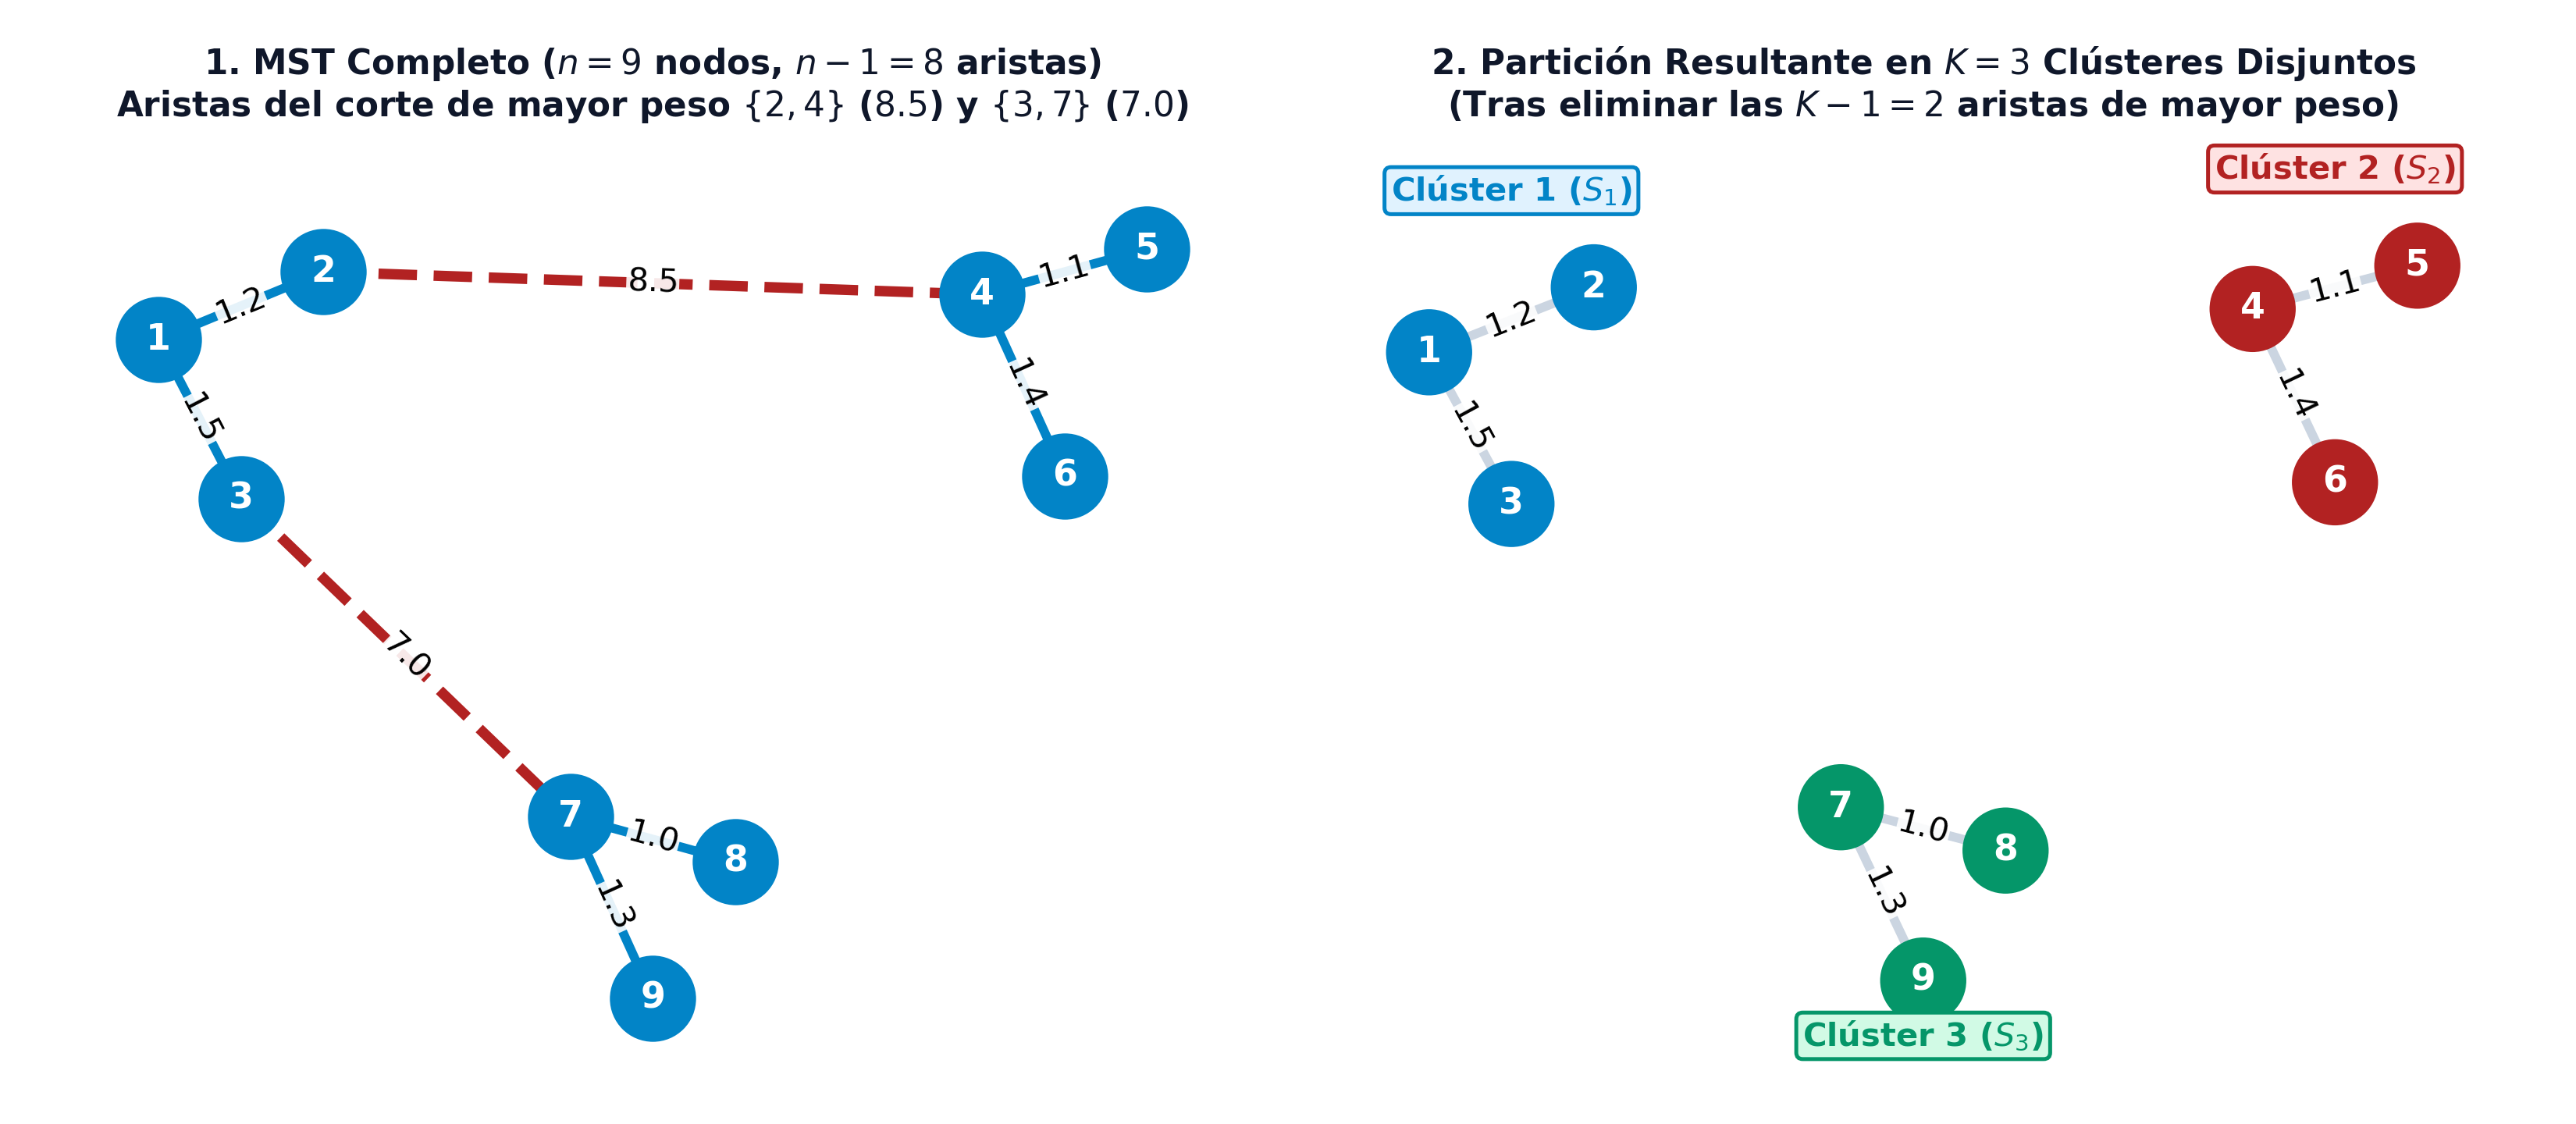
\includegraphics[width=0.85\linewidth,height=\textheight,keepaspectratio]{../images/mst_clustering_ejemplo.png}
\end{center}
\end{frame}

\begin{frame}{Detección de estructuras con geometría no lineal}
\phantomsection\label{detecciuxf3n-de-estructuras-con-geometruxeda-no-lineal}
\begin{itemize}
\tightlist
\item
  \textbf{Estructuras complejas}: Anillos concéntricos (panel izquierdo)
  y dos lunas entrelazadas (panel derecho).
\item
  \textbf{Superioridad del MST}: Mientras \(k\)-medias fracasa al trazar
  hiperplanos lineales rígidos, el MST elimina el puente de mayor
  desemejanza entre estructuras, capturando la topología no convexa
  exacta.
\end{itemize}

\begin{center}
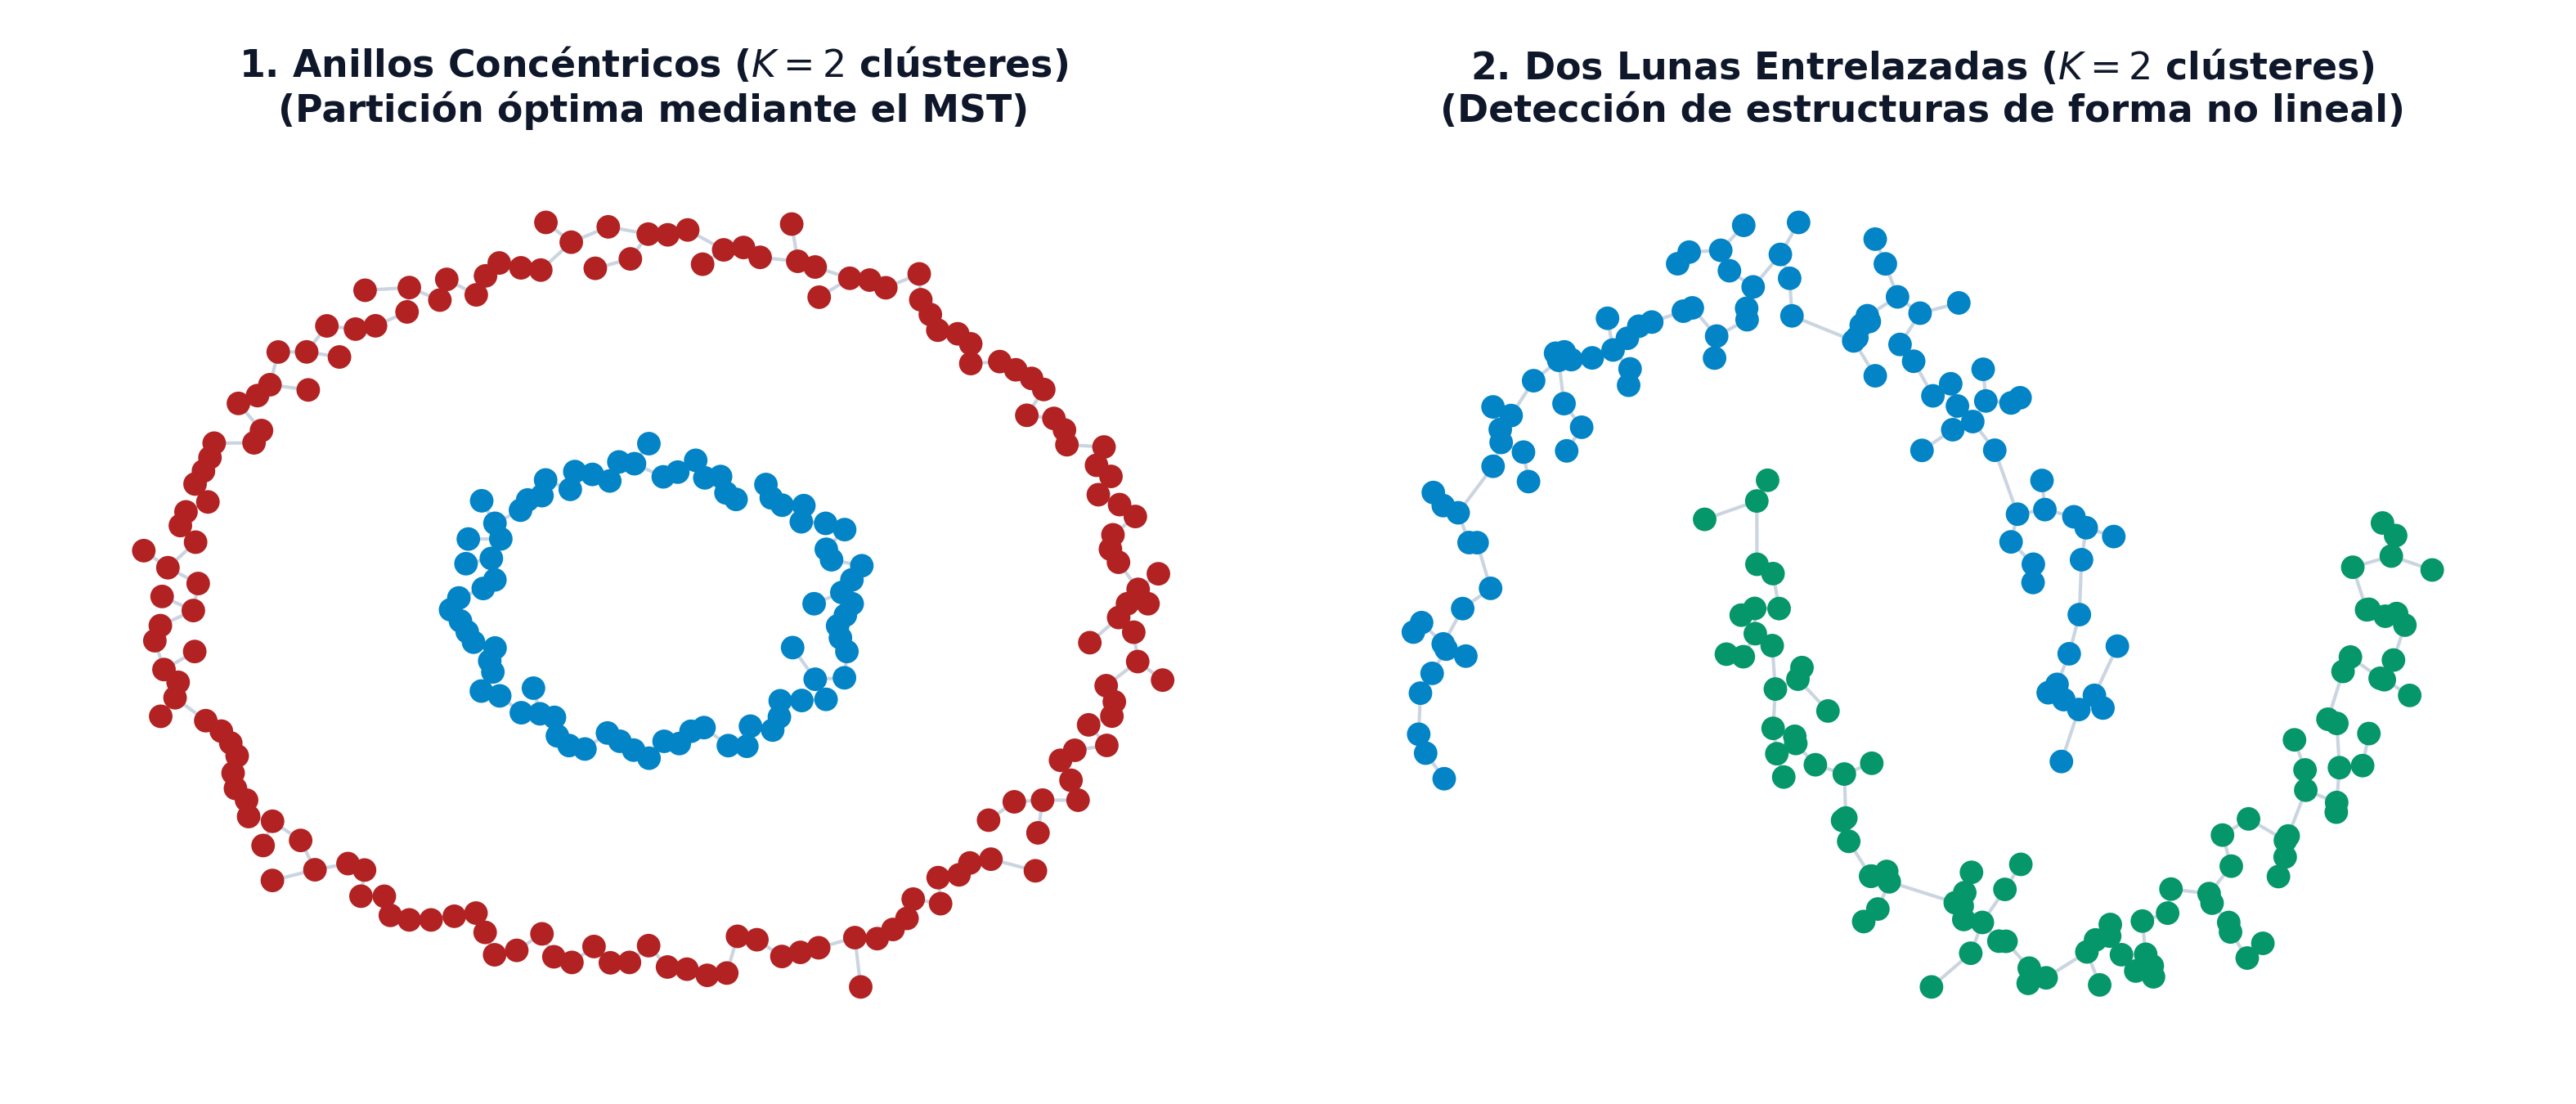
\includegraphics[width=0.85\linewidth,height=\textheight,keepaspectratio]{../images/mst_clustering_complejo.png}
\end{center}
\end{frame}

\begin{frame}{Generalización: Funciones de calidad de partición F}
\phantomsection\label{generalizaciuxf3n-funciones-de-calidad-de-particiuxf3n-f}
\begin{itemize}
\item
  \textbf{Enfoque de Optimización Objetivo}: En lugar de cortar
  únicamente las \(K - 1\) aristas de mayor peso, se define una
  \textbf{función de calidad o validez}
  \(F : \mathcal{X}_\ell \to \mathbb{R}\) que evalúa la bondad de cada
  partición posible \(C(V, E'')\).
\item
  \textbf{Objetivo de Maximización}: Encontrar la partición de la red
  \(C(V, E'') \in \mathcal{X}_\ell\) que maximiza el valor de la función
  de validez \(F\).
\end{itemize}
\end{frame}

\begin{frame}{Maximización de F sobre el MST (Procedimiento Divisivo)}
\phantomsection\label{maximizaciuxf3n-de-f-sobre-el-mst-procedimiento-divisivo}
Dada una red de datos \(G = (V, E, \delta)\) y una función de calidad
\(F\):

\begin{enumerate}
\tightlist
\item
  \textbf{Obtener el MST}: \(T = \text{MST}(G) = (V, E', \delta)\).
\item
  \textbf{Inicializar aristas activas}: \(E'' = E'\).
\item
  \textbf{Bucle de Selección Divisiva}: Para \(i = 1, \dots, K - 1\):

  \begin{itemize}
  \tightlist
  \item
    Identificar
    \(\{u, v\} = \arg\max_{e \in E''} F(C(V, E'' \setminus \{e\}))\).
  \item
    Eliminar la arista seleccionada:
    \(E'' \leftarrow E'' \setminus \{\{u, v\}\}\).
  \end{itemize}
\item
  \textbf{Resultado de la partición}: Devolver la partición óptima
  \(C(V, E'')\).
\end{enumerate}
\end{frame}

\begin{frame}{Funciones de Calidad F: Separación y Variabilidad
Intra-grupo}
\phantomsection\label{funciones-de-calidad-f-separaciuxf3n-y-variabilidad-intra-grupo}
\begin{itemize}
\item
  \textbf{Criterio de mayor longitud (Separación)}: Suma de los
  costes/pesos de las aristas eliminadas del MST: \[
  F(X_1, \dots, X_\ell) = \sum_{i=1}^\ell \sum_{x_j \in X_i} x_j
  \]
\item
  \textbf{Suma de cuadrados intra-grupo negativa (\(-WCSS\))}:
  Minimización de la dispersión de las observaciones respecto a los
  centroides \(\mu_i\): \[
  -WCSS(X_1, \dots, X_\ell) = -\sum_{i=1}^\ell \sum_{x_j \in X_i} \|x_j - \mu_i\|^2
  \]
\end{itemize}
\end{frame}

\begin{frame}{Funciones de Calidad F: Criterio de Información y
Entropía}
\phantomsection\label{funciones-de-calidad-f-criterio-de-informaciuxf3n-y-entropuxeda}
\begin{itemize}
\item
  \textbf{Criterio de Información / Entropía (\(IC\))}: Balancea la
  homogeneidad de los subárboles con la proporción de observaciones: \[
  IC(X_1, \dots, X_\ell) = -d \sum_{i=1}^\ell \frac{n_i}{n} \log \frac{L_i}{n_i} - \sum_{i=1}^\ell \frac{n_i}{n} \log \frac{n_i}{n}
  \] donde \(L_i\) representa la suma de los pesos de las aristas en el
  \(i\)-ésimo subárbol y \(n_i = |X_i|\) es la cardinalidad de dicho
  clúster.
\item
  \textbf{Criterio de dispersión de aristas}: Minimización de la
  desviación típica de las distancias de las aristas intra-clúster.
\end{itemize}
\end{frame}

\begin{frame}{Estrategias aglomerativas e inestabilidades prácticas}
\phantomsection\label{estrategias-aglomerativas-e-inestabilidades-pruxe1cticas}
\begin{tcolorbox}[enhanced jigsaw, toptitle=1mm, opacityback=0, opacitybacktitle=0.6, colback=white, arc=.35mm, bottomrule=.15mm, titlerule=0mm, coltitle=black, breakable, bottomtitle=1mm, left=2mm, title=\textcolor{quarto-callout-warning-color}{\faExclamationTriangle}\hspace{0.5em}{Estrategia aglomerativa y corrección de inestabilidad}, colbacktitle=quarto-callout-warning-color!10!white, rightrule=.15mm, toprule=.15mm, colframe=quarto-callout-warning-color-frame, leftrule=.75mm]

\begin{itemize}
\tightlist
\item
  \textbf{Aproximación aglomerativa}: Comenzar con \(E'' = \emptyset\) e
  ir añadiendo aristas del MST una a una que maximicen la función
  \(F(C(V, E'' \cup \{\{u,v\}\}))\) hasta alcanzar \(K\) componentes
  conexas.
\item
  \textbf{Inconveniente práctico}: Puede formar grupos aislados de muy
  pocas observaciones en las iteraciones iniciales.
\item
  \textbf{Solución}: Incorporar penalizaciones o restricciones basadas
  en el \textbf{índice de Gini} que favorezcan el equilibrio cuando
  exista una disparidad excesiva en la dimensión de los clústeres.
\end{itemize}

\end{tcolorbox}
\end{frame}




\end{document}
